
\section{Thiết kế giao diện}
Giao diện người dùng đóng vai trò quan trọng trong việc mang lại trải nghiệm học tập hiệu quả cho học sinh. Với mục tiêu tạo ra một nền tảng học toán vừa thân thiện vừa hấp dẫn, nhóm đã thiết kế giao diện dựa trên các tiêu chí: dễ sử dụng, trực quan, sáng tạo và phù hợp với lứa tuổi tiểu học. Toàn bộ thiết kế giao diện được trình bày chi tiết tại: \href{https://www.figma.com/design/SoUfs7Sxqv9unjfvdxj9dB/Dino---DACN?node-id=0-1&t=fxbj1E539k6XP6Ww-1}{Figma - Thiết kế Dino Math}.

\subsection{Giao diện Landing Page}
Landing Page của hệ thống \textbf{Dino Math} được thiết kế nhằm mục đích giới thiệu tổng quan về nền tảng học Toán tư duy trực tuyến dành cho học sinh tiểu học, đồng thời thu hút người dùng và khuyến khích đăng ký sử dụng hệ thống. Giao diện Landing Page được thiết kế như \textit{Hình \ref{fig:landingpage}}.

\newline
\vspace{0.5cm}
Giao diện được thiết kế với tông màu tươi sáng kết hợp với các hình minh họa sinh động cũng như hoạt ảnh (Animation) được tạo bằng Lottielab, qua đó tạo cảm giác thân thiện và phù hợp với đối tượng người dùng là trẻ em, đồng thời vẫn đảm bảo tính rõ ràng và dễ sử dụng đối với phụ huynh.

\newline
\vspace{0.5cm}
Phần \textbf{Đầu trang (Header)} bao gồm logo nhận diện thương hiệu của hệ thống và các nút chức năng \textit{Đăng ký} và \textit{Đăng nhập}. Các thành phần này được bố trí hợp lý, giúp người dùng dễ dàng truy cập vào hệ thống.

\newline
\vspace{0.5cm}
Khu vực \textbf{Giới thiệu chính (Hero Section)} nằm ở vị trí trung tâm của trang, hiển thị khẩu hiệu \textit{``Học mà chơi, chơi mà học!''}, thể hiện rõ định hướng giáo dục của hệ thống. Bên dưới là đoạn mô tả ngắn giới thiệu Dino Math là nền tảng học Toán tư duy trực tuyến dành cho học sinh tiểu học. Nút kêu gọi hành động \textit{``Dùng thử ngay''} được thiết kế nổi bật nhằm khuyến khích người dùng trải nghiệm hệ thống.

\newline
\vspace{0.5cm}
Tiếp theo là khu vực \textbf{Các tính năng nổi bật}, trong đó các chức năng chính của hệ thống được trình bày dưới dạng các thẻ nội dung kèm biểu tượng minh họa. Các tính năng bao gồm học Toán thông qua bài tập tương tác, kết hợp học và chơi với các minigame Toán học, so tài với người dùng khác, theo dõi tiến trình học tập, tăng cường sự tương tác giữa phụ huynh và học sinh, cũng như gợi ý lộ trình học tập phù hợp với chương trình học thực tế.

\newline
\vspace{0.5cm}
Cuối trang là \textbf{Chân trang (Footer)}, cung cấp thông tin giới thiệu ngắn gọn về hệ thống, các liên kết điều hướng nhanh, biểu tượng mạng xã hội và thông tin bản quyền. Ngoài ra, landing page còn hiển thị các công nghệ và nền tảng hỗ trợ hệ thống nhằm tăng mức độ tin cậy cho người dùng.

\begin{figure}[H]
	\centering
	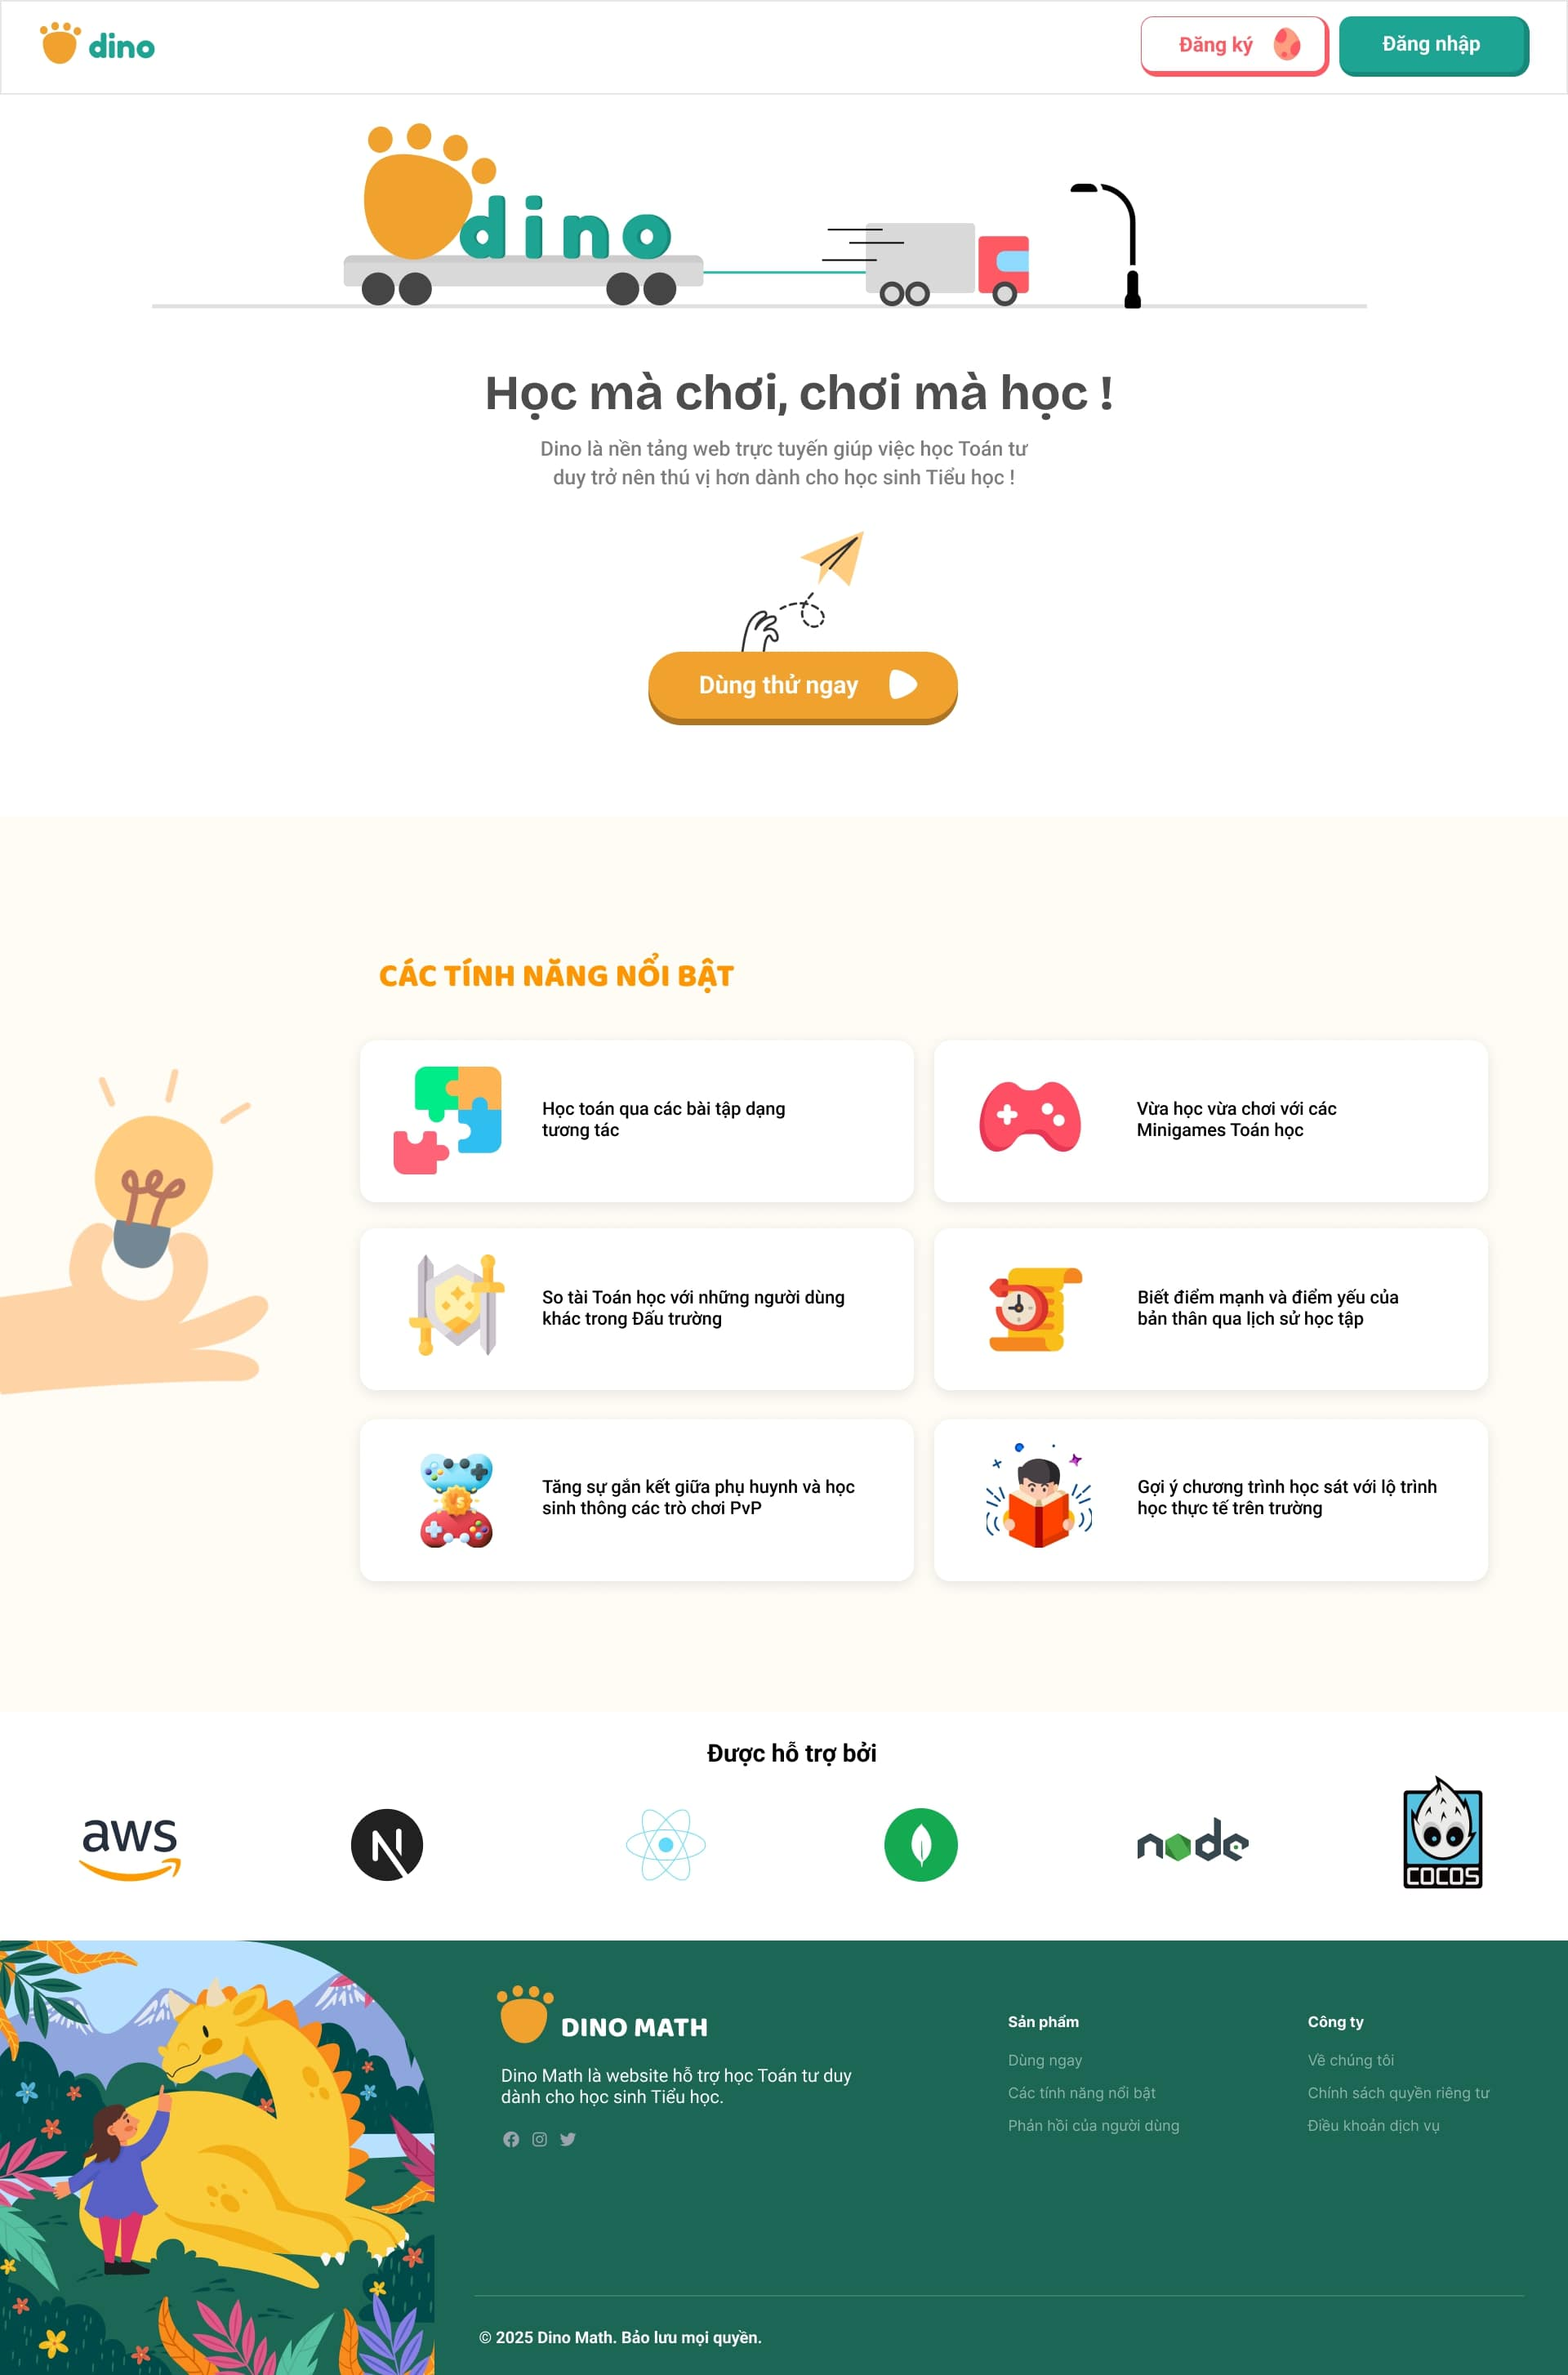
\includegraphics[width=0.9\textwidth]{Image/UI/LandingPage.jpg}
	\vspace{0.6cm}
	\caption{Landing Page}
	\label{fig:landingpage}
\end{figure}

\subsection{Giao diện đăng nhập và đăng ký tài khoản}
\subsubsection{Giao diện đăng nhập}
\label{subsubsec:login}
\begin{itemize}
	\item \textbf{Mục đích:} Cho phép người dùng xác thực tài khoản thông qua email và mật khẩu để truy cập và sử dụng các dịch vụ của hệ thống.
	\item \textbf{Mô tả:} 
	\begin{itemize}
		\item Giao diện đăng nhập ở giữa màn hình sẽ được hiển thị khi người dùng chọn tab \textit{Đăng nhập} ở thanh điều hướng bên trái.
		\item Có 2 phương thức để đăng nhập: Đăng nhập bằng tài khoản hệ thống hoặc Đăng nhập bằng tài khoản Google.
		\begin{itemize}
			\item Đối với chức năng Đăng nhập bằng tài khoản hệ thống, người dùng phải nhập thông tin đăng nhập vào các field \textit{Email} và \textit{Mật khẩu} như \textit{Hình \ref{fig:login}}. Nếu người dùng quên mật khẩu, có thể bấm vào link \textit{Quên mật khẩu} để truy cập vào trang \textbf{Lấy lại mật khẩu} được mô tả ở mục \ref{subsec:resetpassword}.
			Nút \textit{Đăng nhập} chỉ được enable khi giá trị của các field khác rỗng. Sau khi bấm đăng nhập, hệ thống sẽ tiến hành gửi request về backend để
			xác thực người dùng. Nếu thành công, người dùng sẽ được điều hướng về giao diện mặc định tùy theo loại tài khoản (đối với tài khoản học sinh, giao diện mặc định là \textbf{Trang chủ} được mô tả ở mục \ref{subsubsec:studenthome}, còn đối với phụ huynh là \textbf{Trang thống kê tổng quan} được mô tả ở mục \ref{subsubsec:parenthome}). Nếu thất bại, lỗi cụ thể sẽ được hiển thị dưới dạng toast message để thông báo cho người dùng như \textit{Hình \ref{fig:wrongpassword}}. Ngoài ra, đối với tài khoản học sinh, sau khi đăng nhập lần đầu tiên, người dùng sẽ được điều hướng đến giao diện \textbf{Onboarding} được mô tả ở mục \ref{subsec:onboarding} để cập nhật hồ sơ cá nhân.
			\begin{figure}[H]
				\centering
				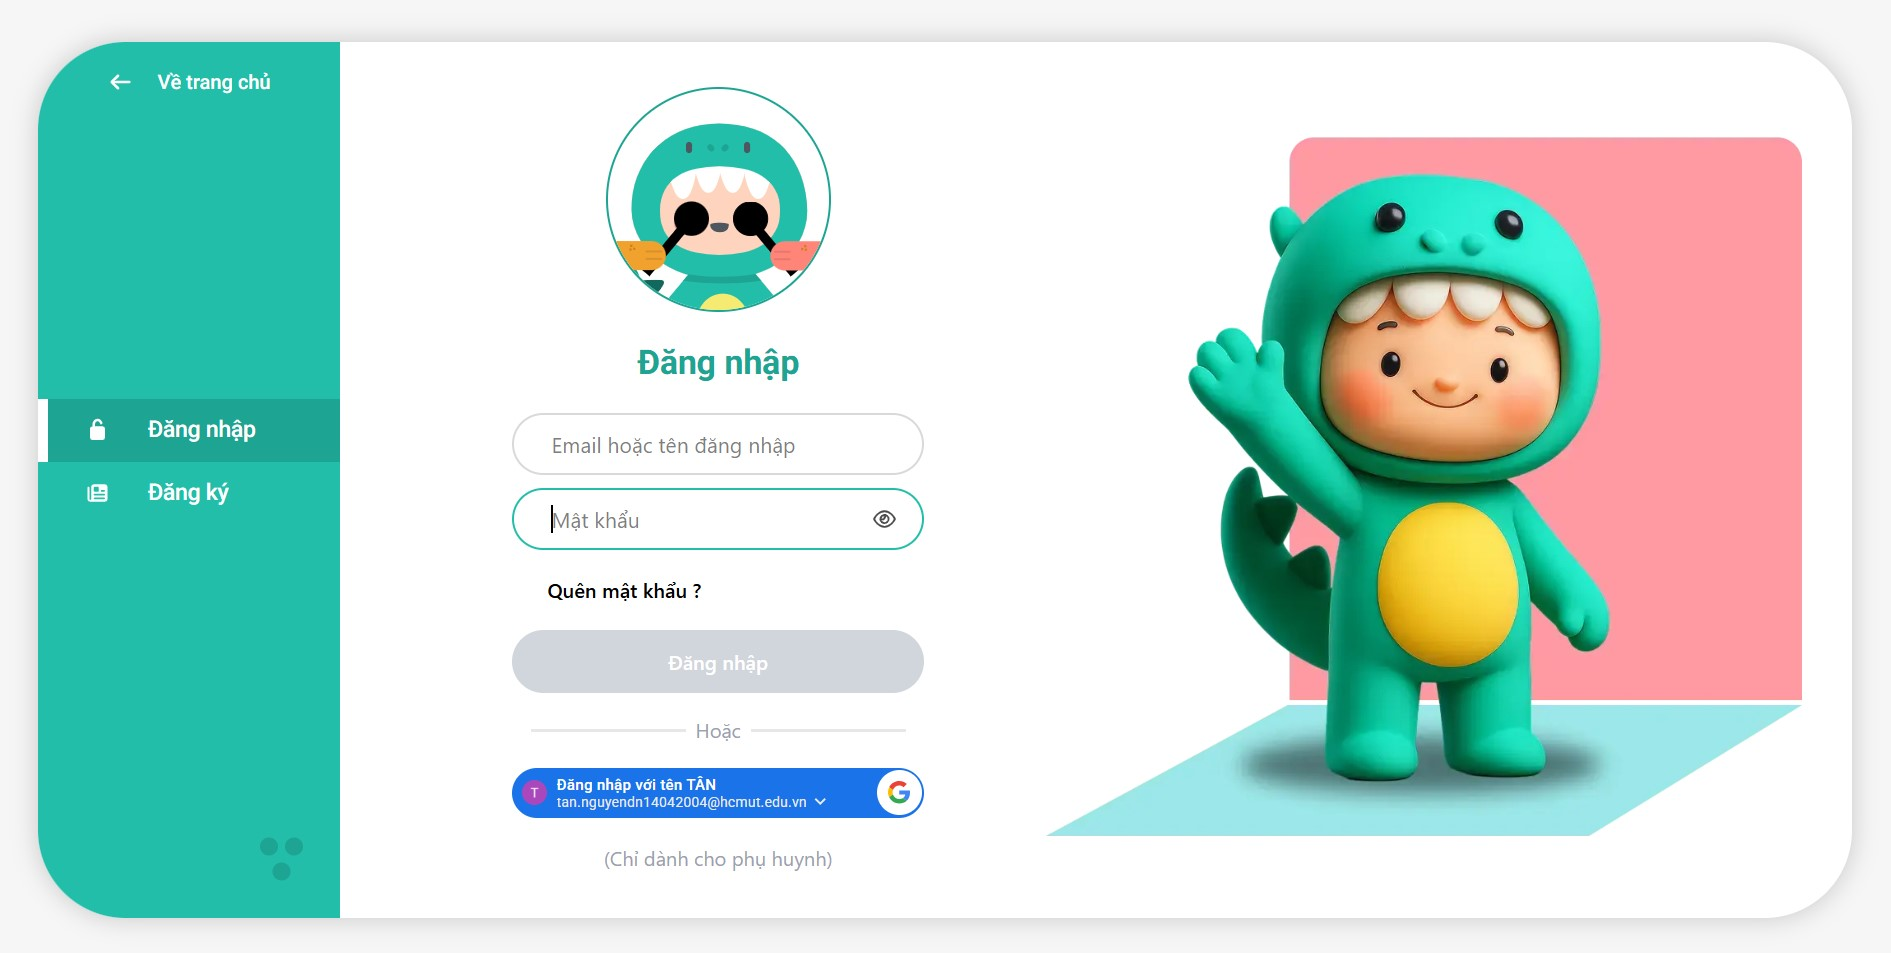
\includegraphics[width=0.9\textwidth]{Image/UI/Auth/Login.jpg}
				\vspace{0.6cm}
				\caption{Giao diện đăng nhập}
				\label{fig:login}
			\end{figure}
			\begin{figure}[H]
				\centering
				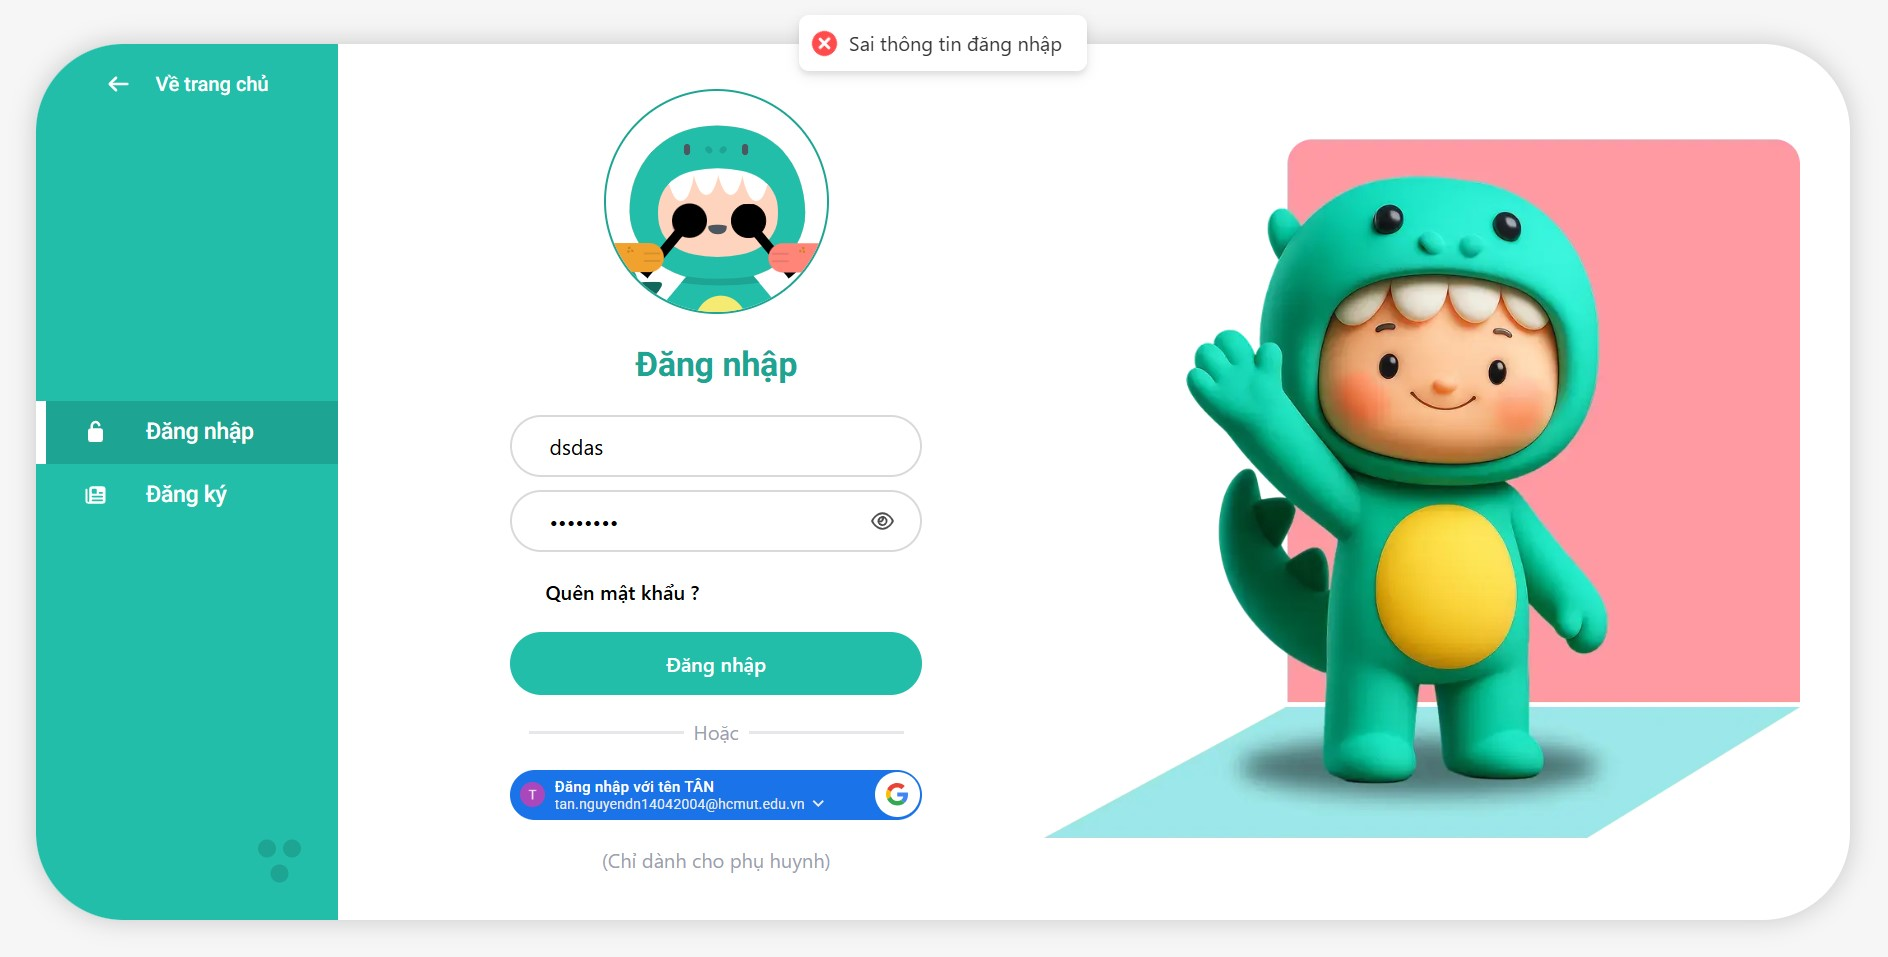
\includegraphics[width=0.9\textwidth]{Image/UI/Auth/LoginError.jpg}
				\vspace{0.6cm}
				\caption{Lỗi sai thông tin đăng nhập}
				\label{fig:wrongpassword}
			\end{figure}
			\item Đối với chức năng đăng nhập bằng Google (chỉ dành cho Phụ huynh), người dùng sẽ bấm vào nút \textit{Đăng nhập bằng Google}. Sau đó, người dùng thực hiện các thao tác đăng nhập bằng tài khoản Google trên cửa sổ mới. Nếu thành công, người dùng được điều hướng tới trang chủ của mình.
			\begin{figure}[H]
				\centering
				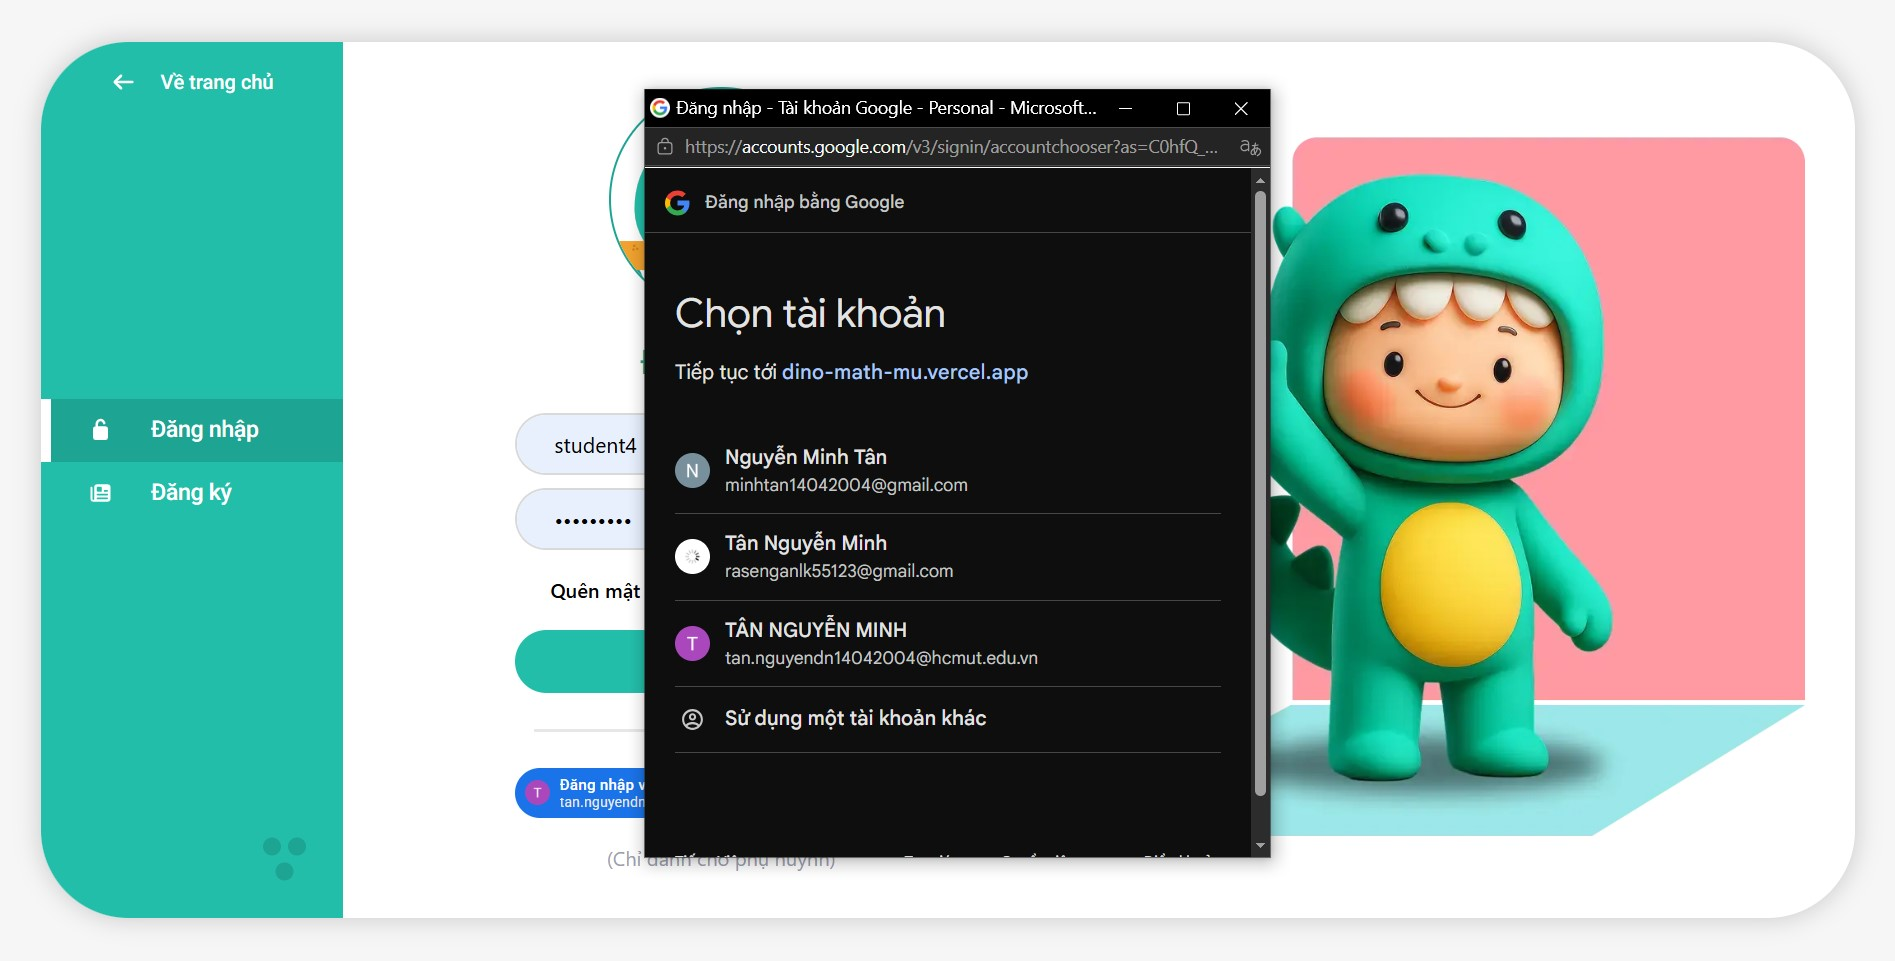
\includegraphics[width=0.9\textwidth]{Image/UI/Auth/OAuth.jpg}
				\vspace{0.6cm}
				\caption{Giao diện đăng nhập bằng Google}
				\label{fig:oauth}
			\end{figure}
		\end{itemize}
	\end{itemize}
\end{itemize}

\subsubsection{Giao diện đăng ký tài khoản}
\begin{itemize}
	\item \textbf{Mục đích:} Cho phép người dùng đăng ký tài khoản mới.
	\item \textbf{Mô tả:} Giao diện đăng ký sẽ được hiển thị khi người dùng chọn tab \textit{Đăng ký} ở thanh điều hướng bên trái. Giao diện đăng ký tài khoản bao gồm 2 bước:
	\begin{itemize}
		\item \textbf{Bước 1 - Chọn loại tài khoản}: Người dùng cần chọn 1 trong 2 loại tài khoản mà mình muốn tạo bao gồm: Phụ huynh hoặc Học sinh. Giao diện của bước này được mô tả như thiết kế như \textit{Hình \ref{fig:rolepick}} bên dưới. 
		\begin{figure}[H]
			\centering
			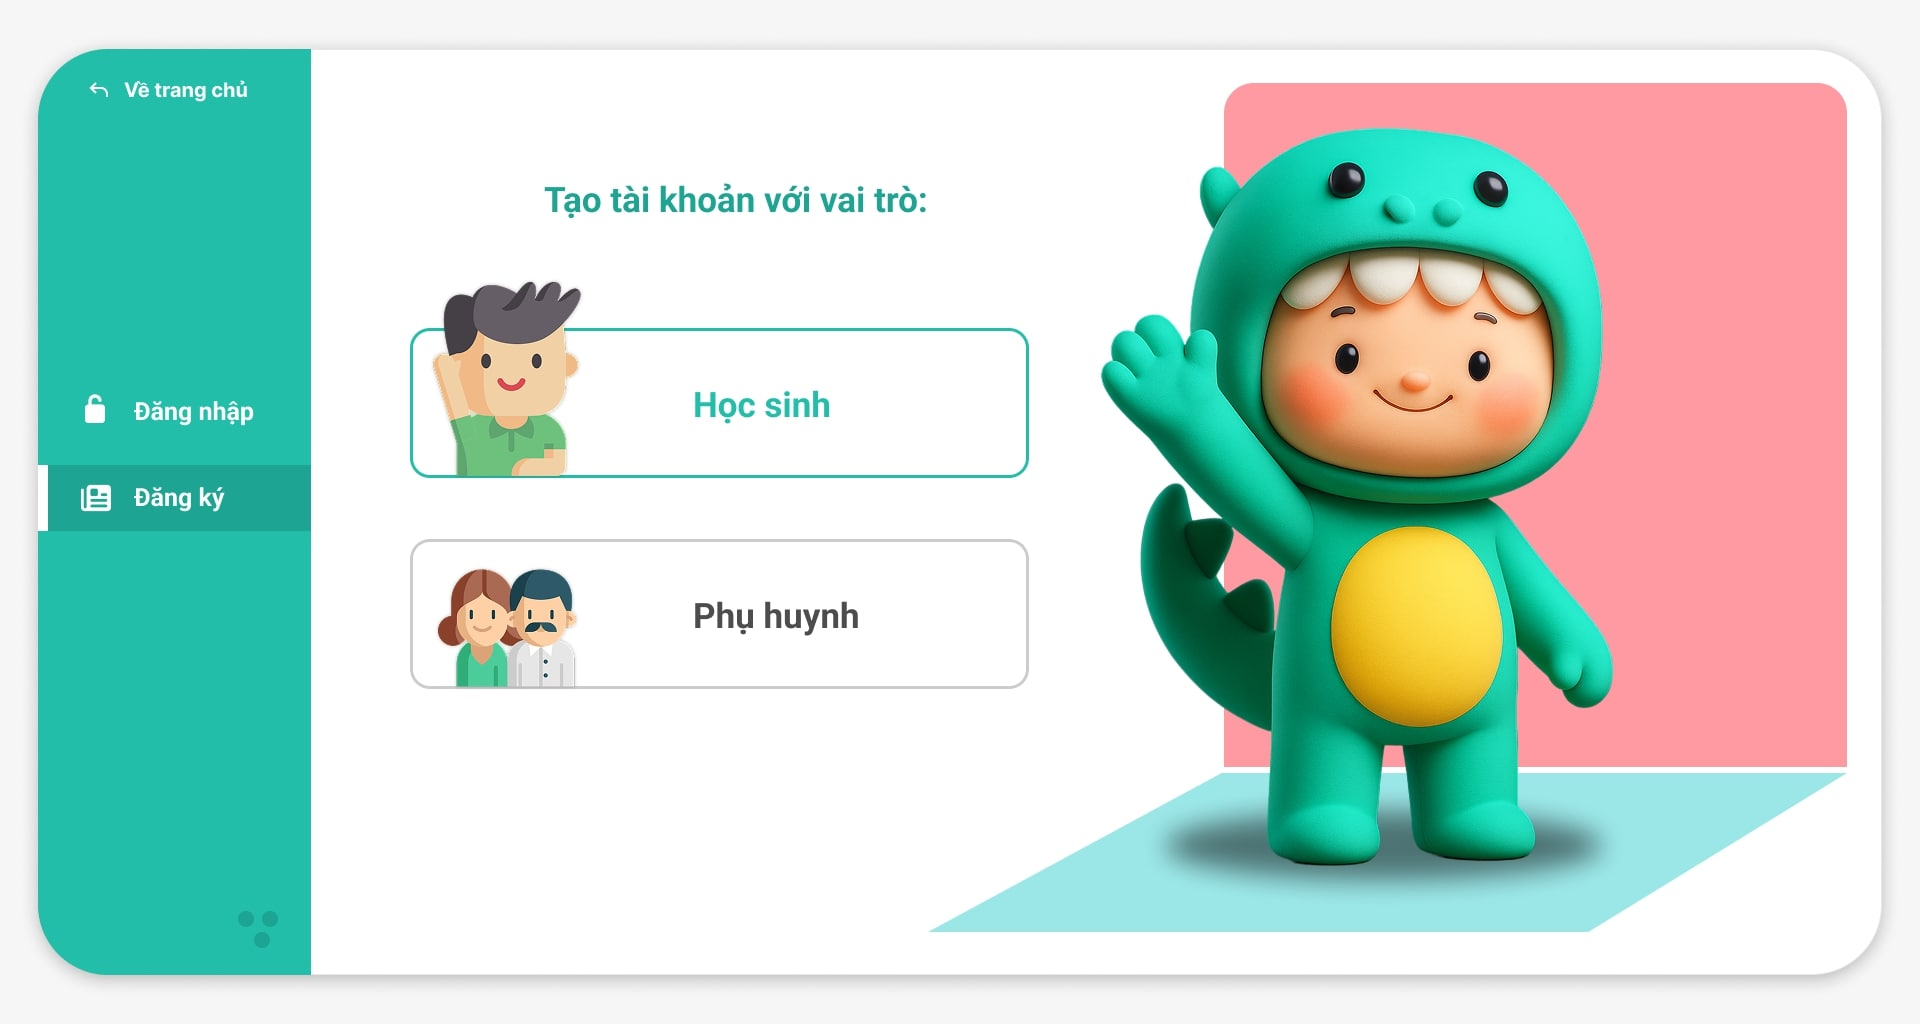
\includegraphics[width=0.9\textwidth]{Image/UI/Auth/SignUpPage-RolePicking.jpg}
			\vspace{0.6cm}
			\caption{Giao diện đăng ký tài khoản - Chọn loại tài khoản}
			\label{fig:rolepick}
		\end{figure}
		
		\item \textbf{Bước 2 - Nhập thông tin đăng ký}: Người dùng cần nhập  các thông tin bao gồm: Email (đối với phụ huynh) hoặc Tên tài khoản (đối với học sinh), Họ và tên, Mật khẩu và Xác nhận mật khẩu. Đối với thông tin về Họ và tên, thông tin này chỉ xuất hiện khi người dùng chọn đăng ký tài khoản Phụ huynh, còn đối với Học sinh, thông tin này sẽ được bổ sung sau ở giao diện \textbf{Onboarding} được mô tả ở mục \ref{subsec:onboarding}.
		Nút \textit{Đăng ký} chỉ được enable khi các điều kiện sau được thỏa mãn:
		\begin{itemize}
			\item Giá trị của tất cả các field khác rỗng.
			\item Mật khẩu có ít nhất 8 ký tự, trong đó phải chứa chữ cái in hoa, chữ thường, số và ký tự đặc biệt.
			\item Mật khẩu và Xác nhận mật khẩu phải trùng khớp.
		\end{itemize}
		Giao diện của bước 2 được thiết kế như \textit{Hình \ref{fig:regstudent}} và \textit{Hình \ref{fig:regparent}} bên dưới.
		\begin{figure}[H]
			\centering
			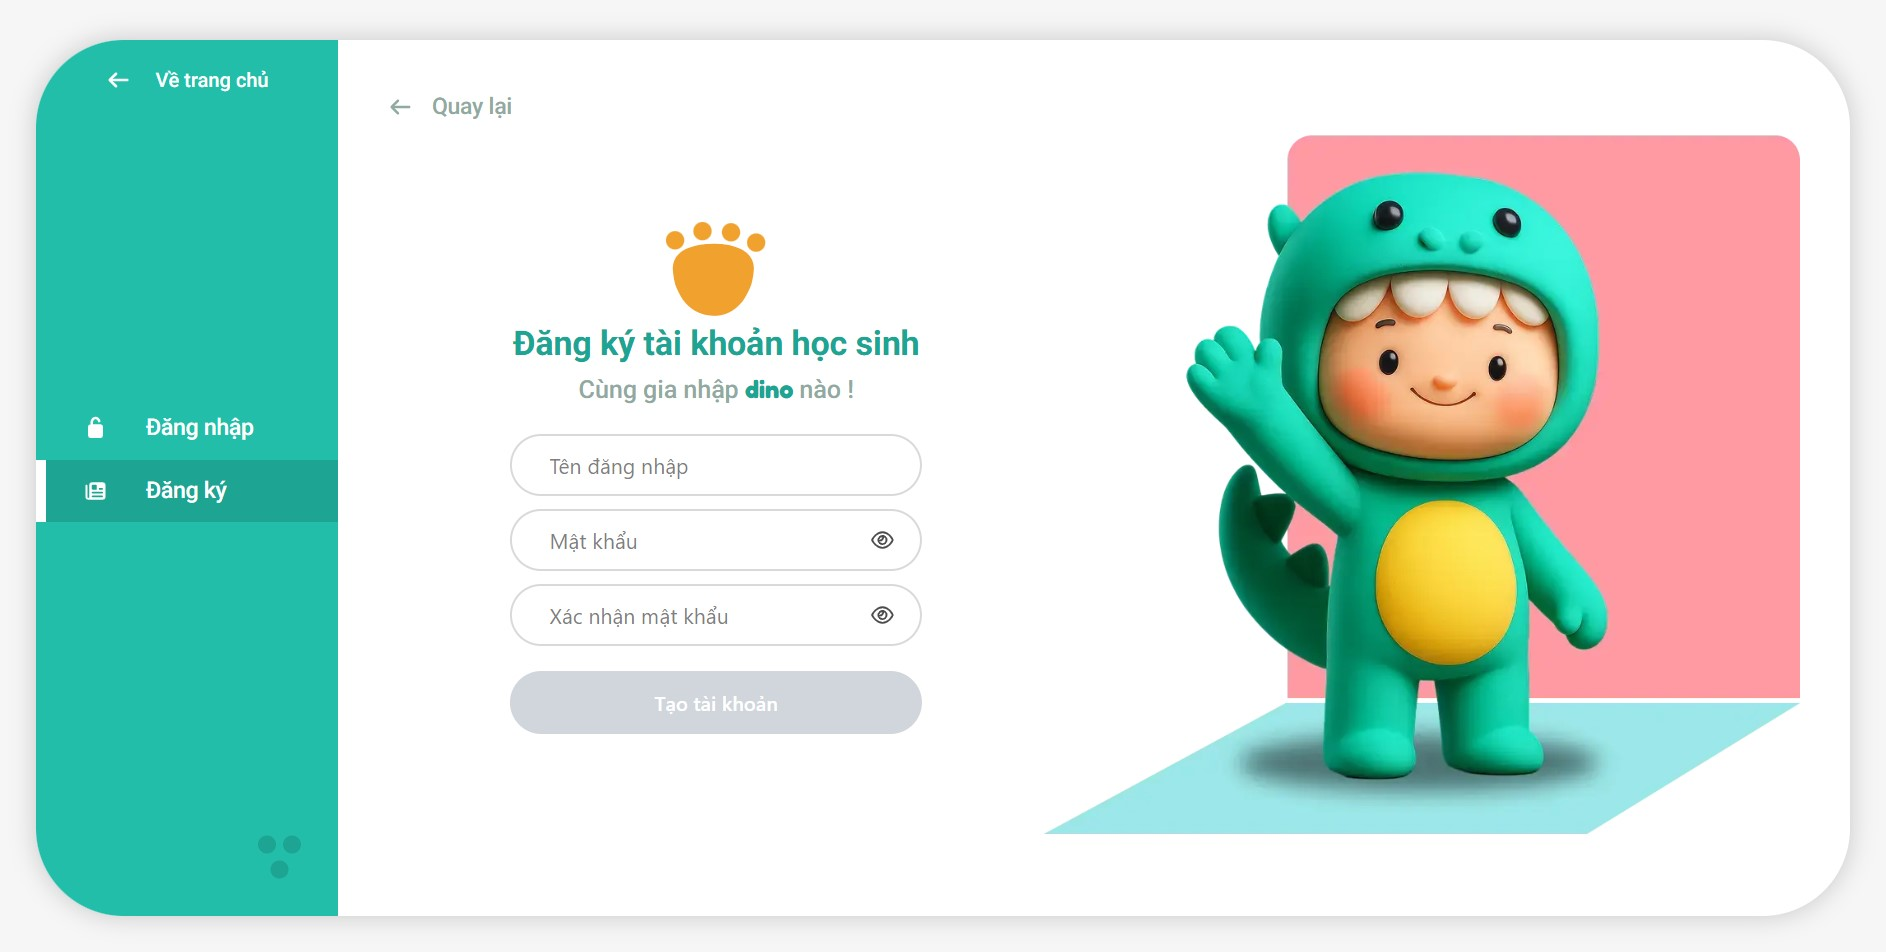
\includegraphics[width=0.9\textwidth]{Image/UI/Auth/StudentRegister.jpg}
			\vspace{0.6cm}
			\caption{Giao diện đăng ký tài khoản - Học sinh}
			\label{fig:regstudent}
		\end{figure}
		\begin{figure}[H]
			\centering
			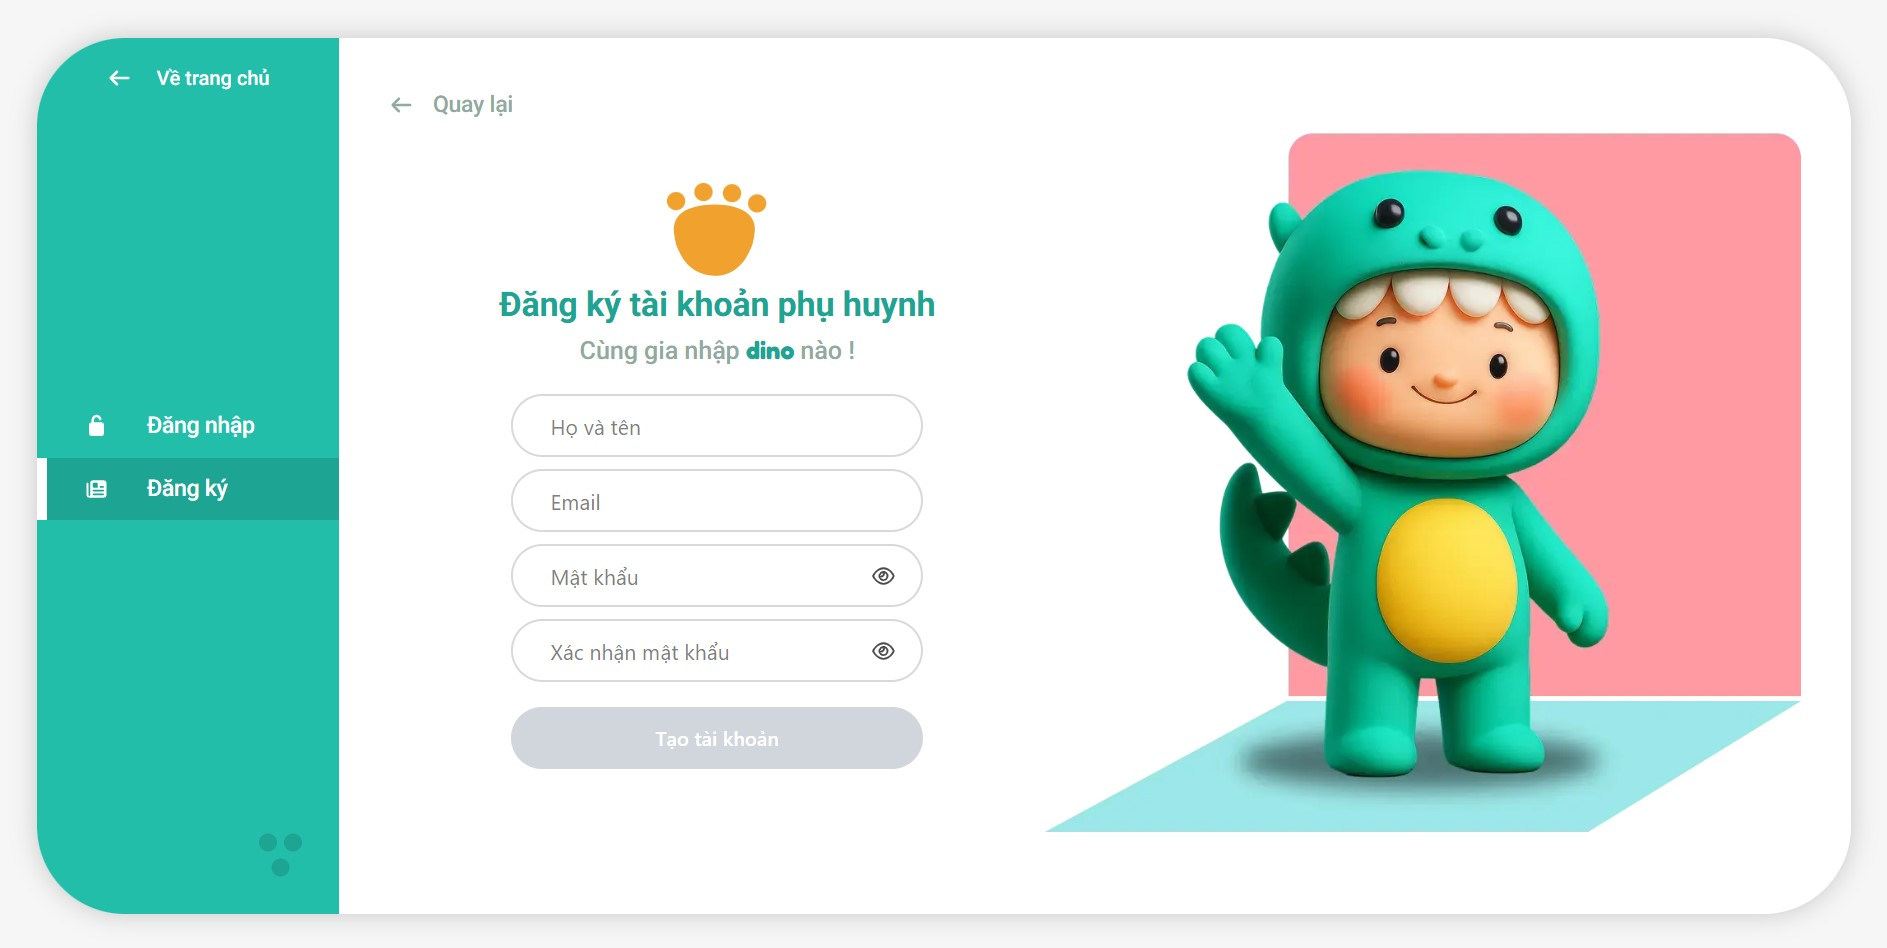
\includegraphics[width=0.9\textwidth]{Image/UI/Auth/ParentRegister.jpg}
			\vspace{0.6cm}
			\caption{Giao diện đăng ký tài khoản - Phụ huynh}
			\label{fig:regparent}
		\end{figure}
		
		\item \textbf{Bước 3 - Bấm đăng ký tài khoản}: Sau khi tất cả thông tin hợp lệ, người dùng có thể bấm nút đăng ký tài khoản để tiến hành tạo tài khoản mới. Thông báo đăng ký thành công hoặc thất bại sẽ được hiển thị dưới dạng toast message được thiết kế như \textit{Hình \ref{fig:regerror}} và \textit{Hình \ref{fig:success}} bên dưới.
	\end{itemize}
	\begin{figure}[H]
		\centering
		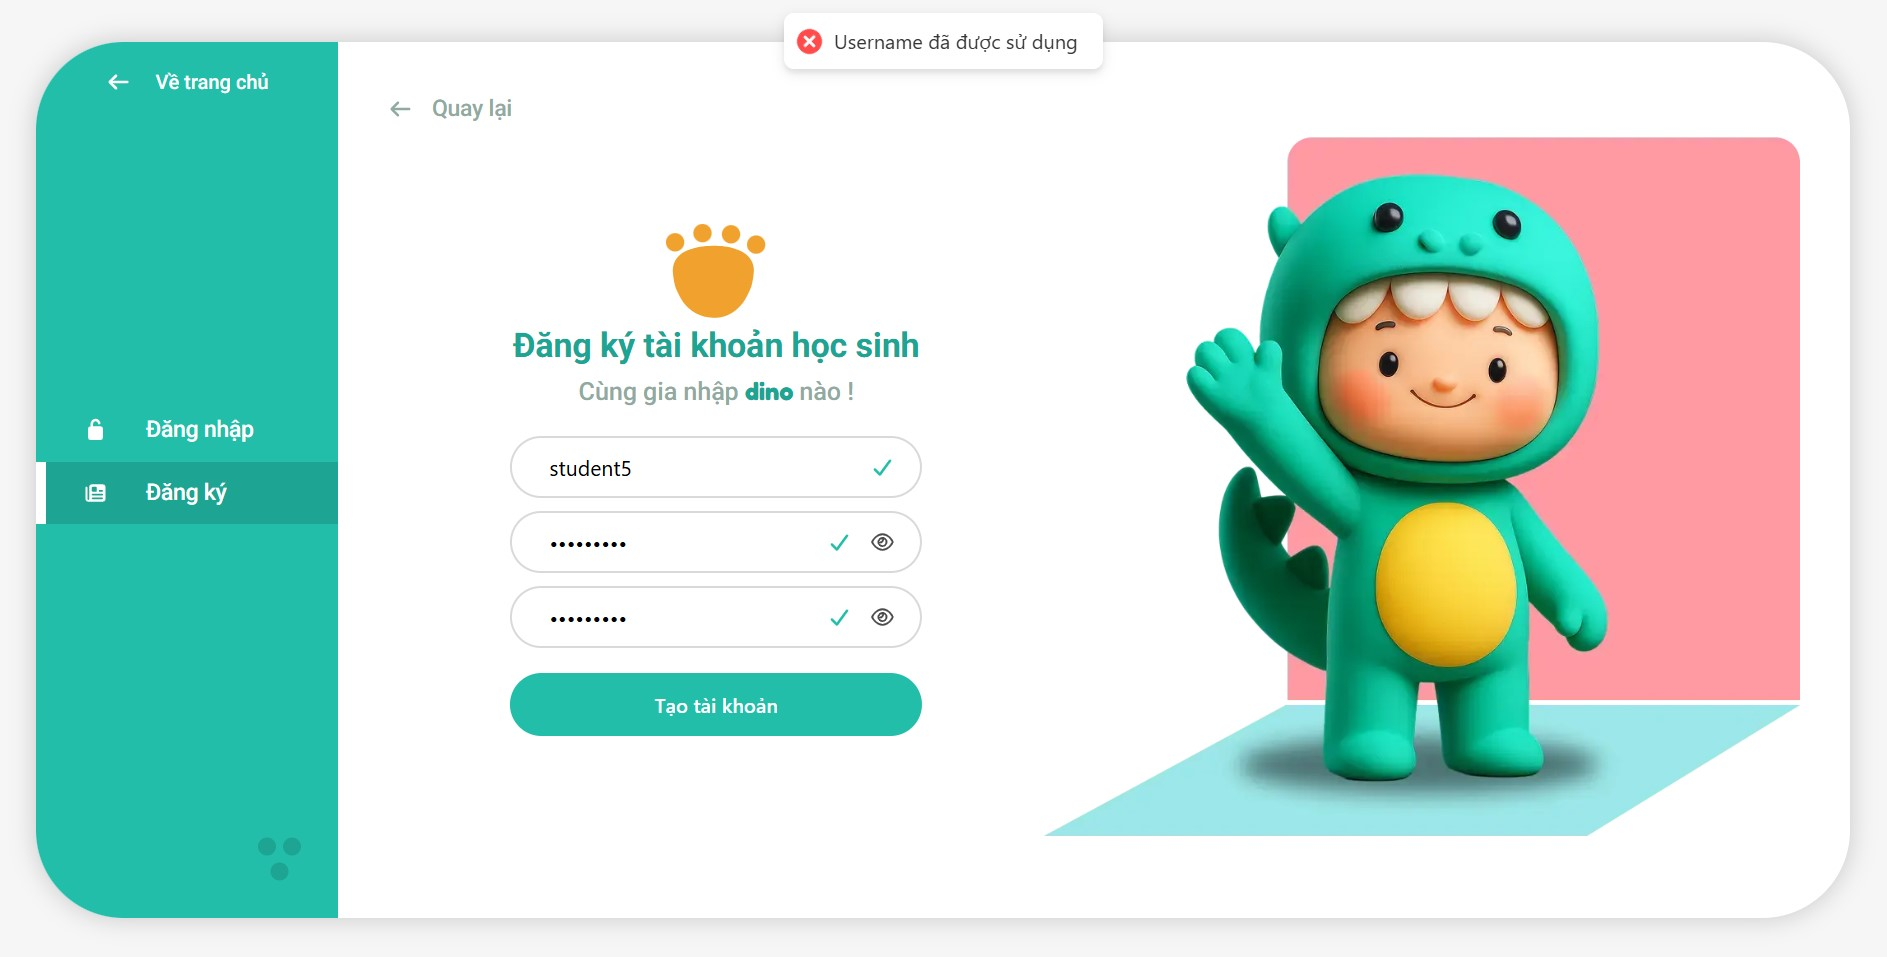
\includegraphics[width=0.9\textwidth]{Image/UI/Auth/UserExist.jpg}
		\vspace{0.6cm}
		\caption{Giao diện đăng ký tài khoản - Lỗi username đã được sử dụng}
		\label{fig:regerror}
	\end{figure}
	\begin{figure}[H]
		\centering
		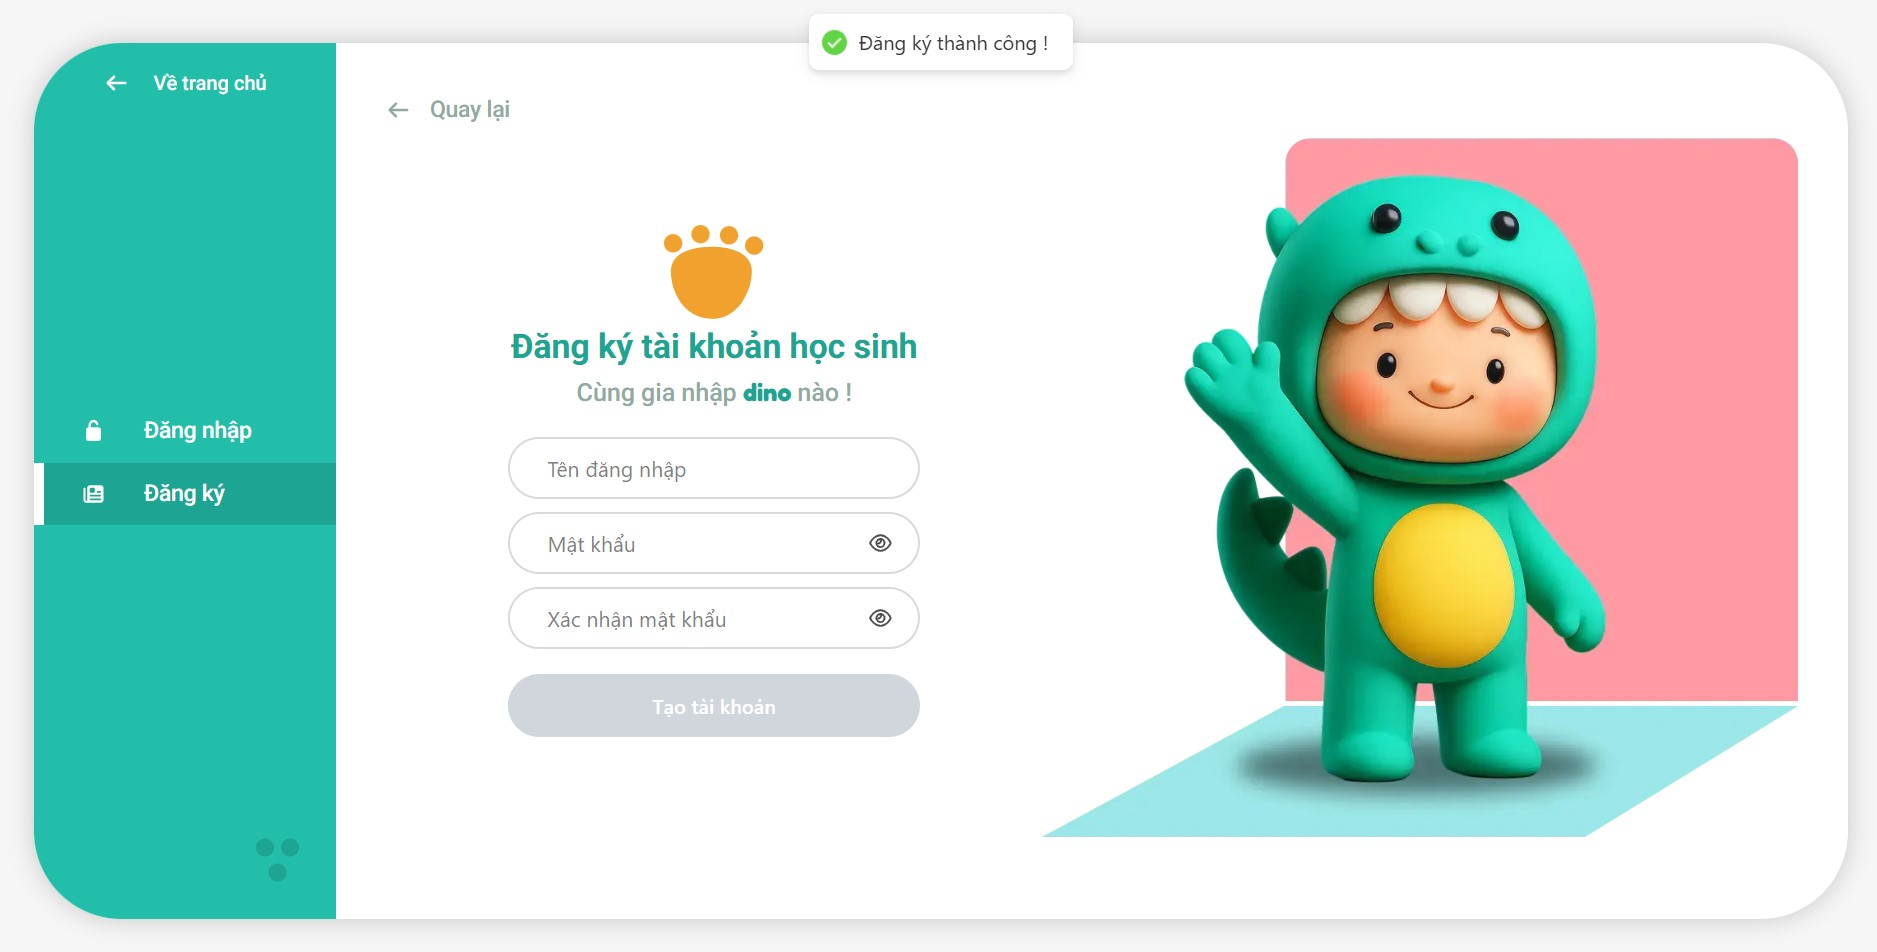
\includegraphics[width=0.9\textwidth]{Image/UI/Auth/RegisterSuccess.jpg}
		\vspace{0.6cm}
		\caption{Giao diện đăng ký tài khoản thành công}
		\label{fig:success}
	\end{figure}
\end{itemize}}

\subsection{Giao diện Onboarding}
\label{subsec:onboarding}
\begin{itemize}
	\item \textbf{Mục đích:} 
	\begin{itemize}
		\item Cho phép người dùng là Học sinh cập nhật thông tin của mình khi đăng nhập lần đầu tiên. 
		\item Cung cấp giao diện tương tác với Linh vật động của hệ thống, tạo cảm giác hứng thú và gần gũi đối với đối tượng người dùng chính là học sinh Tiểu học.
	\end{itemize}
	\item \textbf{Mô tả:} 
	Giao diện Onboarding bao gồm 3 bước như sau:
	\begin{itemize}
		\item \textbf{Bước 1 - Nhập thông tin cá nhân bao gồm họ tên và khối lớp (1-5)}: Học sinh cần nhập Họ và tên cũng như chọn Khối lớp mà mình đang học ở ô dropdown. Nút Tiếp tục chỉ được enable khi tất cả các thông tin đã được điền. Giao diện của bước 1 được thiết kế như \textit{Hình \ref{fig:onboarding}} bên dưới.
		\begin{figure}[H]
			\centering
			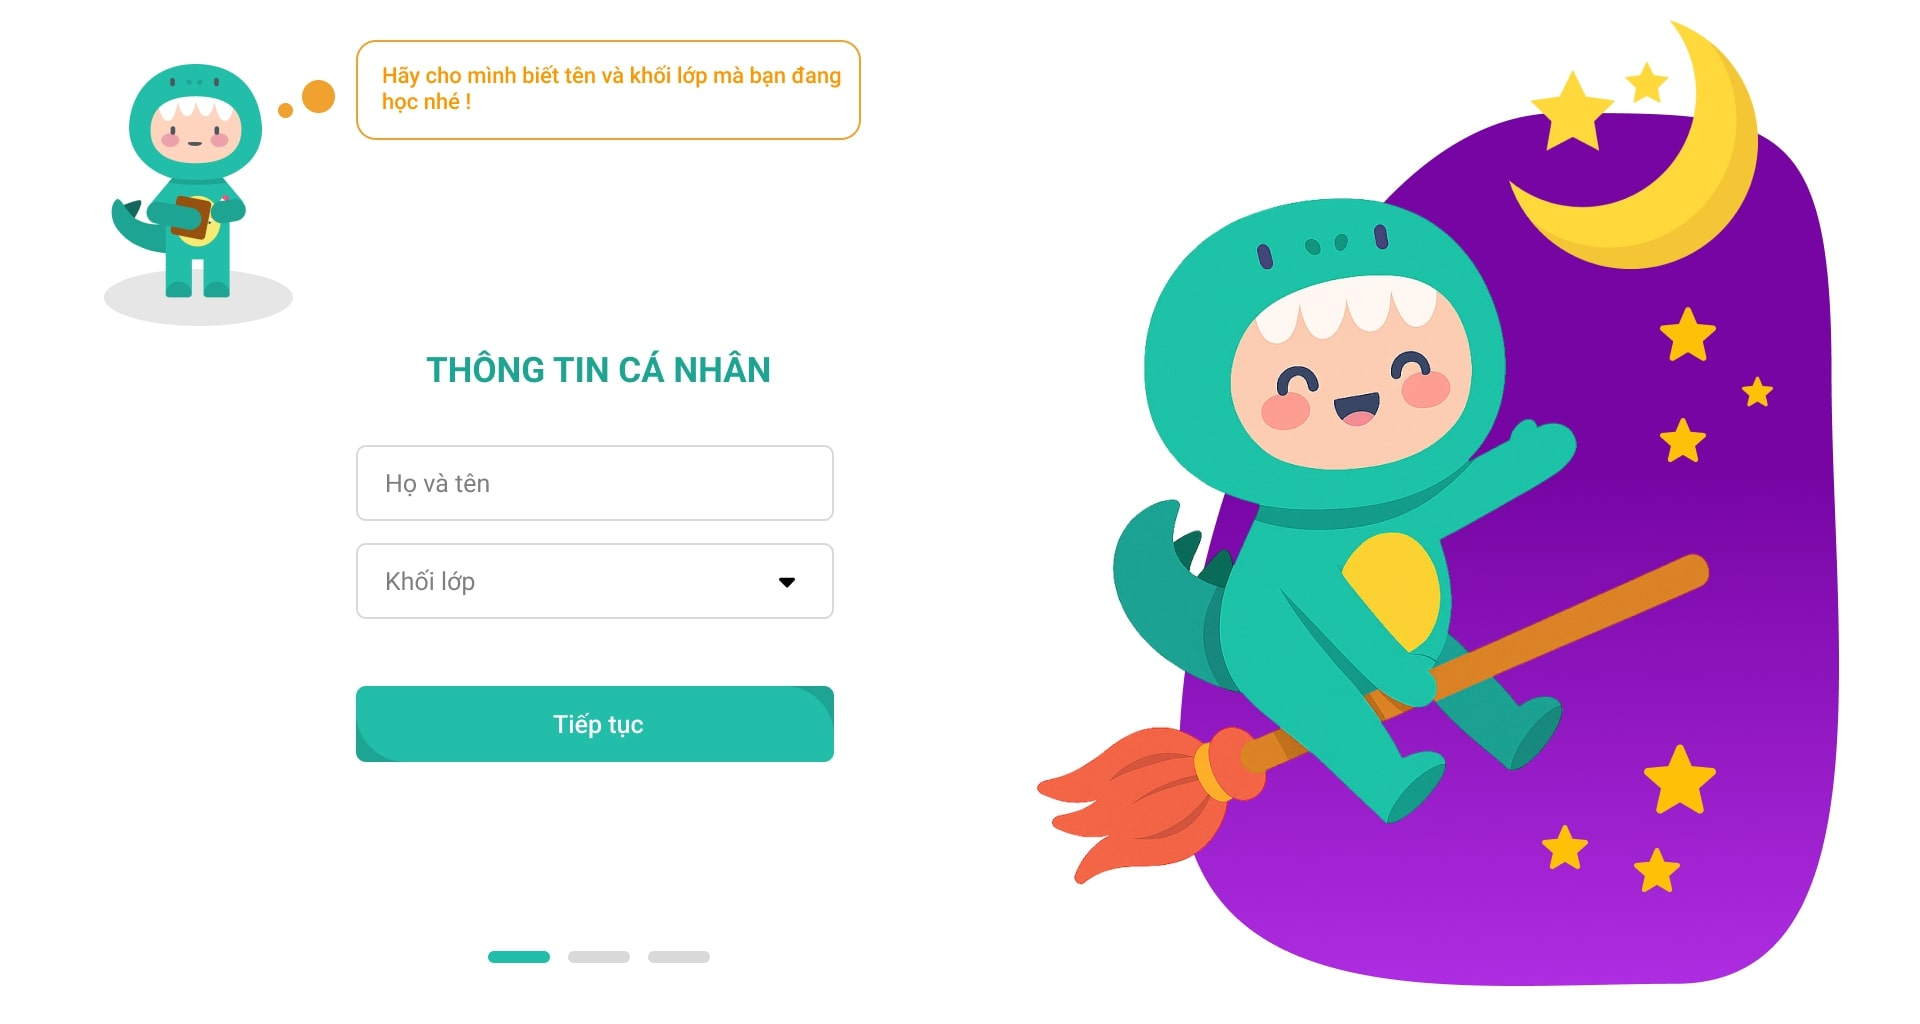
\includegraphics[width=0.9\textwidth]{Image/UI/Auth/Onboarding-Info.jpg}
			\vspace{0.6cm}
			\caption{Giao diện Onboarding - Nhập Họ tên và Khối lớp}
			\label{fig:onboarding}
		\end{figure}
		
		\item \textbf{Bước 2 - Cập nhật ảnh đại diện}: Học sinh có thể chọn ảnh đại diện có sẵn của hệ thống hoặc ảnh tự chọn. Giao diện của bước 2 được thiết kế như \textit{Hình \ref{fig:avatar}} bên dưới.
		\begin{figure}[H]
			\centering
			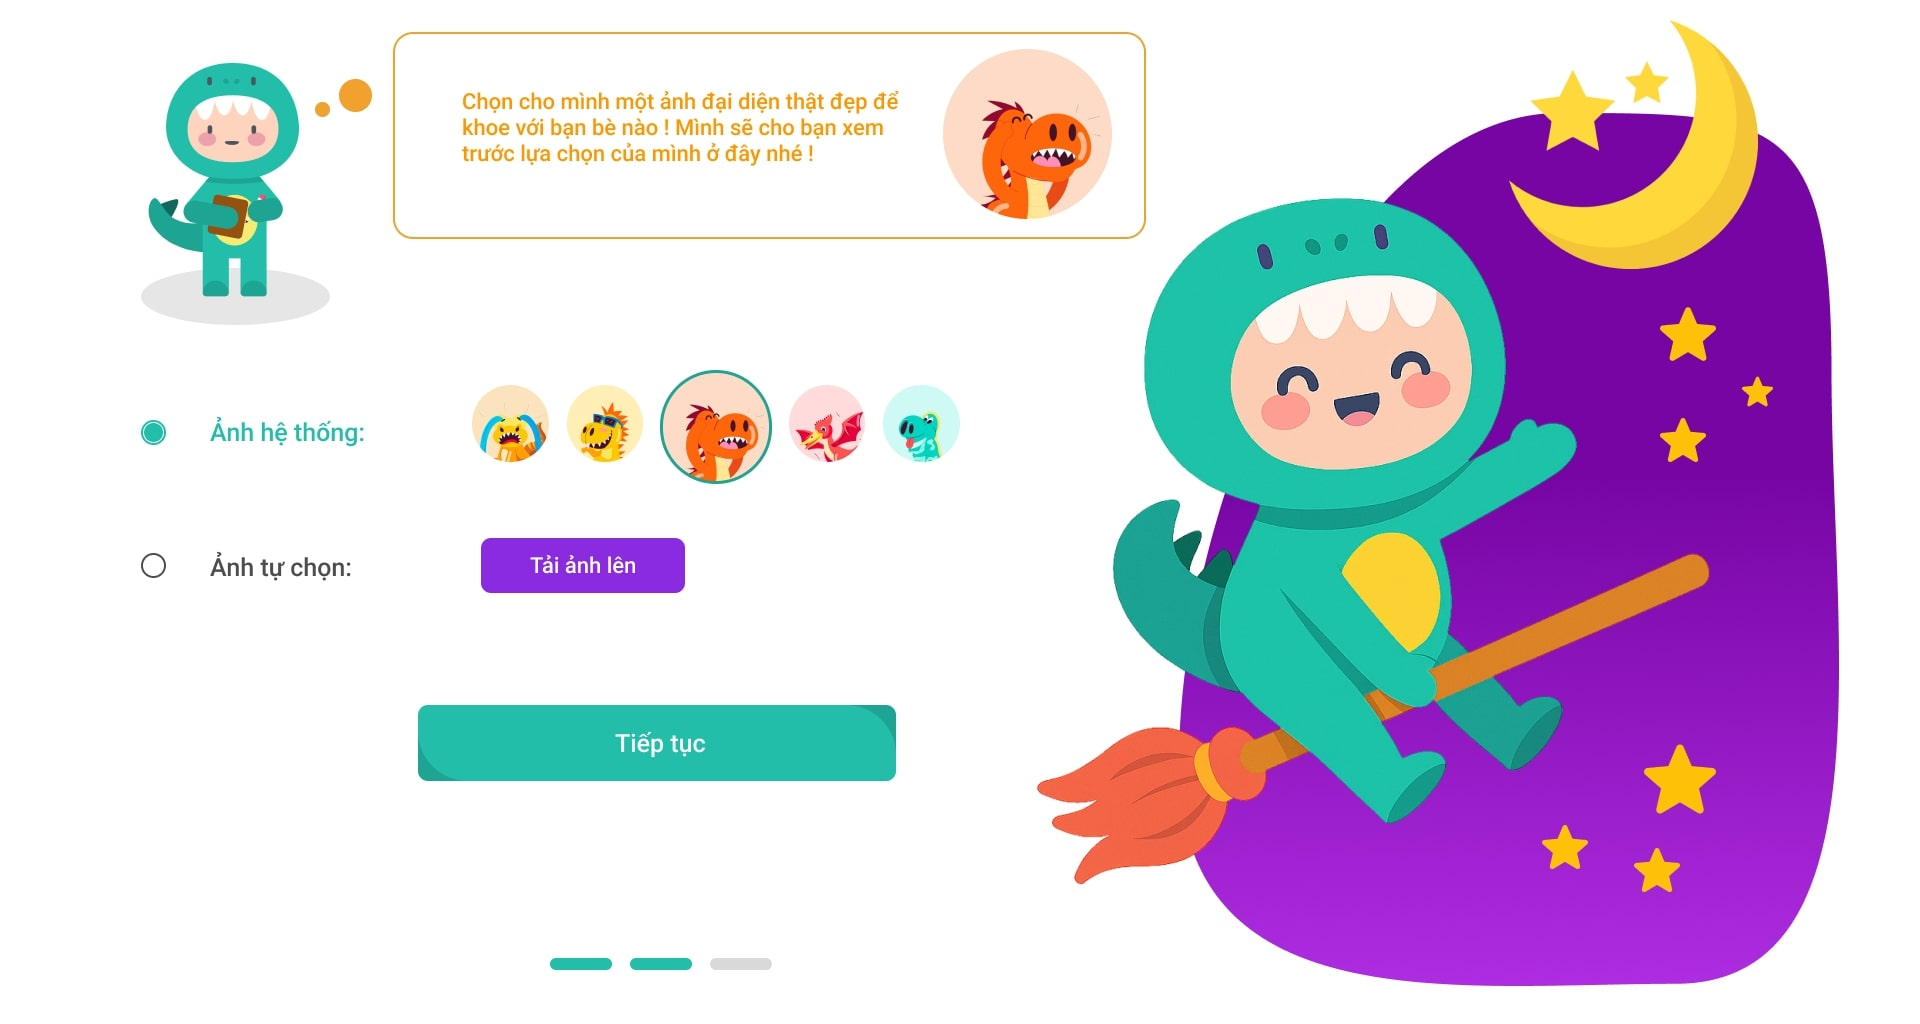
\includegraphics[width=0.9\textwidth]{Image/UI/Auth/Onboarding-Avatar.jpg}
			\vspace{0.6cm}
			\caption{Giao diện Onboarding - Cập nhật ảnh đại diện}
			\label{fig:avatar}
		\end{figure}
		
		\item \textbf{Bước 3 - Nhập mã liên kết tài khoản}: Hệ thống sẽ được tổ chức thành các Family (Gia đình), mỗi gia đình được quản lý bởi một tài khoản Phụ huynh duy nhất. Mã liên kết hay mã mời là mã mà Phụ huynh gửi cho Học sinh để liên kết vào Family của Phụ huynh đó. Ở bước Nhập mã liên kết, Học sinh có thể để trống field này và có thể thực hiện liên kết sau khi đã đăng nhập. Giao diện của bước 3 được thiết kế như \textit{Hình \ref{fig:link}} bên dưới.
		\begin{figure}[H]
			\centering
			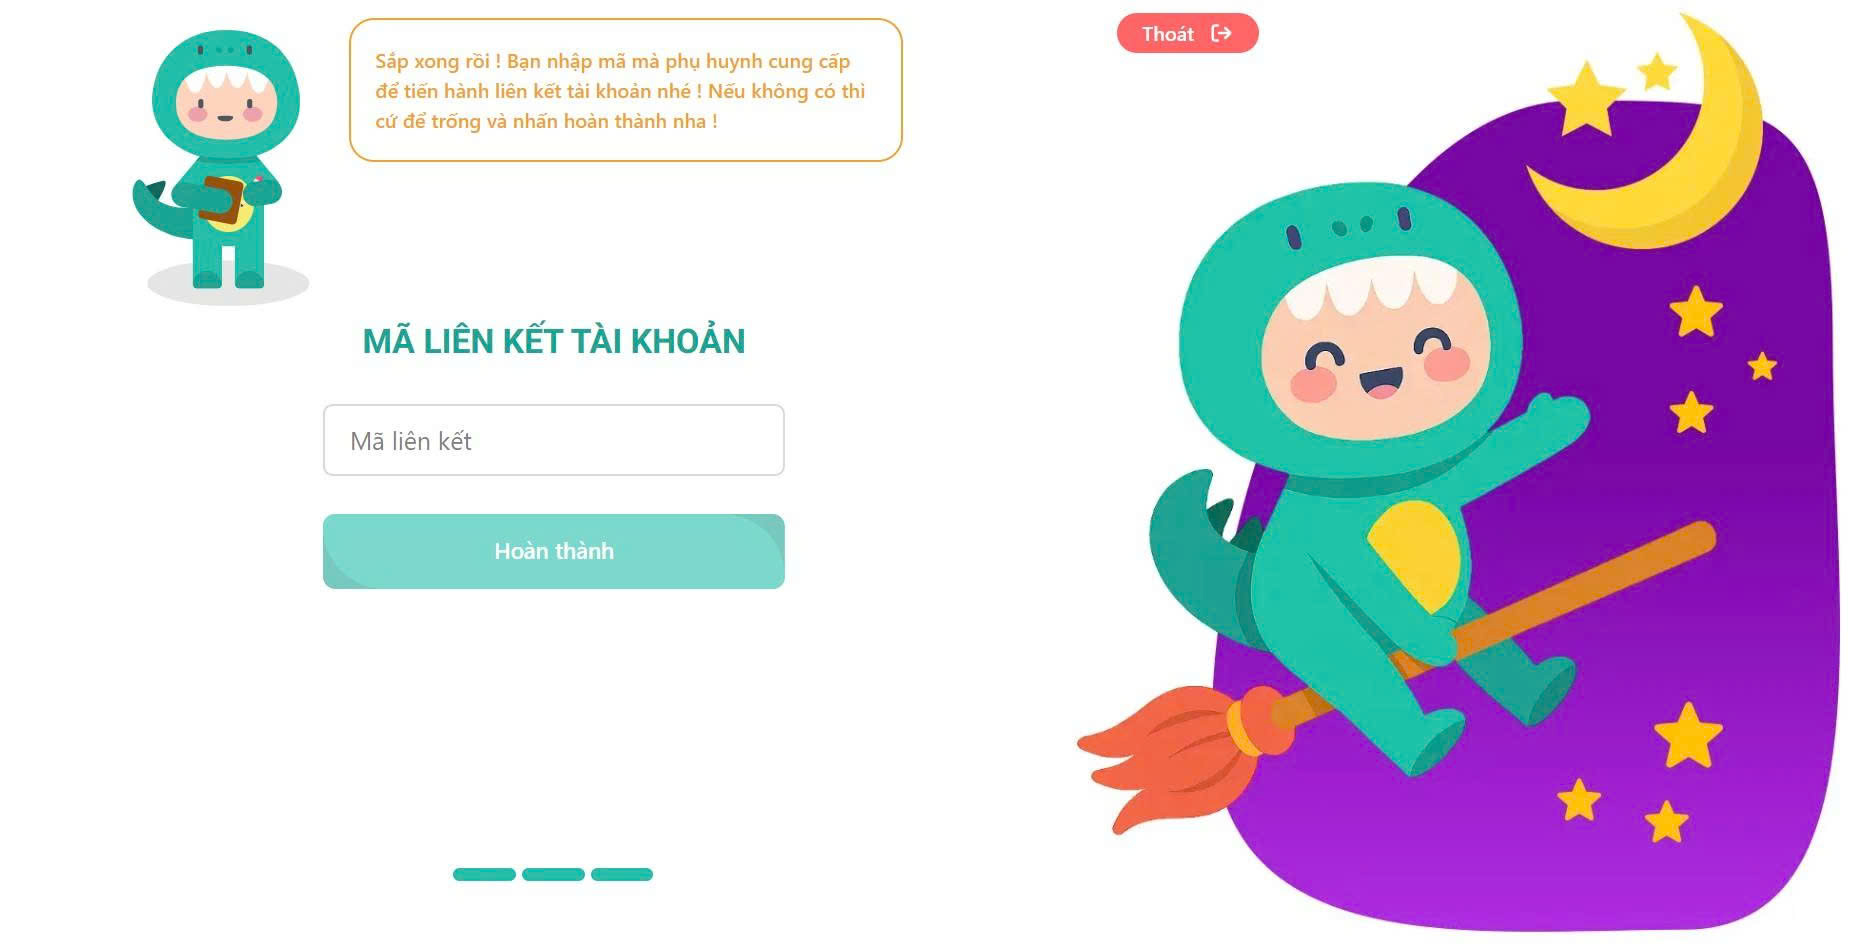
\includegraphics[width=0.9\textwidth]{Image/UI/Auth/Onboarding-InviteCode.jpg}
			\vspace{0.6cm}
			\caption{Giao diện Onboarding - Nhập mã liên kết tài khoản}
			\label{fig:link}
		\end{figure}
		\item Sau khi bấm hoàn thành, học sinh sẽ được điều hướng về \textbf{Trang chủ} của mình được mô tả ở mục \ref{subsubsec:studenthome}.
	\end{itemize}
\end{itemize}

\newpage
\subsection{Giao diện Lấy lại mật khẩu}
\label{subsec:resetpassword}
\begin{itemize}
	\item \textbf{Mục đích:} Giúp người dùng lấy lại mật khẩu thông qua xác thực OTP được gửi đến email.
	\item \textbf{Mô tả:} 
	Khi người dùng bấm vào link \textit{Quên mật khẩu} ở giao diện đăng nhập, trang lấy lại mật khẩu sẽ được hiển thị. Giao diện Lấy lại mật khẩu bao gồm 3 bước như sau:
	\begin{itemize}
		\item \textbf{Bước 1 - Gửi OTP qua email}: Người dùng cần nhập địa chỉ Email (nếu là phụ huynh) và Tên tài khoản (nếu là học sinh) vào ô trống và bấm nút \textit{Gửi mã xác thực}. Sau đó, một email kèm OTP sẽ được gửi đến địa chỉ email của phụ huynh. Nếu người dùng là học sinh, cần liên hệ với phụ huynh để nhận OTP. Giao diện của bước 1 được thiết kế như \textit{Hình \ref{fig:sendotp}} bên dưới.
		\begin{figure}[H]
			\centering
			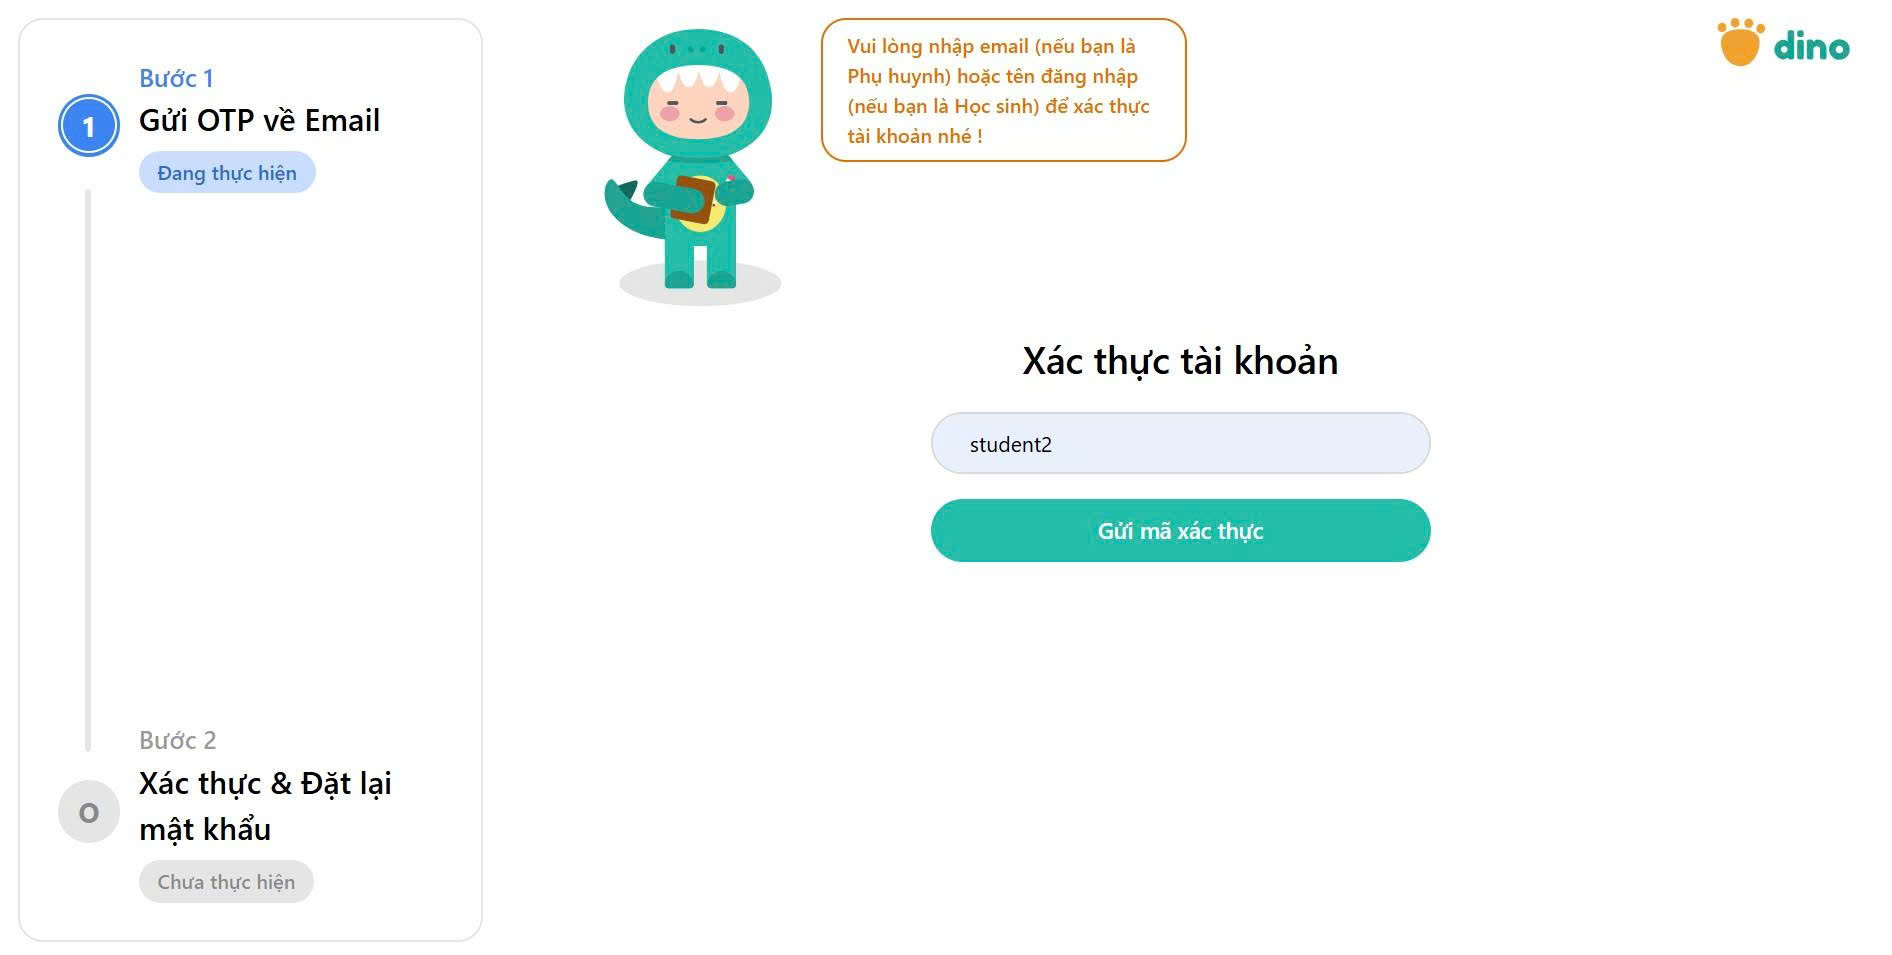
\includegraphics[width=0.9\textwidth]{Image/UI/Auth/PasswordReset1.jpg}
			\vspace{0.6cm}
			\caption{Giao diện Lấy lại mật khẩu - Bước 1}
			\label{fig:sendotp}
		\end{figure}
		
		\item \textbf{Bước 2 - Xác thực OTP và đổi mật khẩu}: Người dùng cần nhập mã OTP được cung cấp, sau đó điền mật khẩu mới của mình vào các textbox tương ứng.  Nút \textit{Đổi mật khẩu} chỉ được enable khi:
		\begin{itemize}
			\item Giá trị của tất cả các field khác rỗng.
			\item Mật khẩu có ít nhất 8 ký tự, trong đó phải chứa chữ cái in hoa, chữ thường, số và ký tự đặc biệt.
			\item Mật khẩu và Xác nhận mật khẩu phải trùng khớp.
		\end{itemize}
		Giao diện của bước 2 được thiết kế như \textit{Hình \ref{fig:inputotp}} bên dưới.
		\begin{figure}[H]
			\centering
			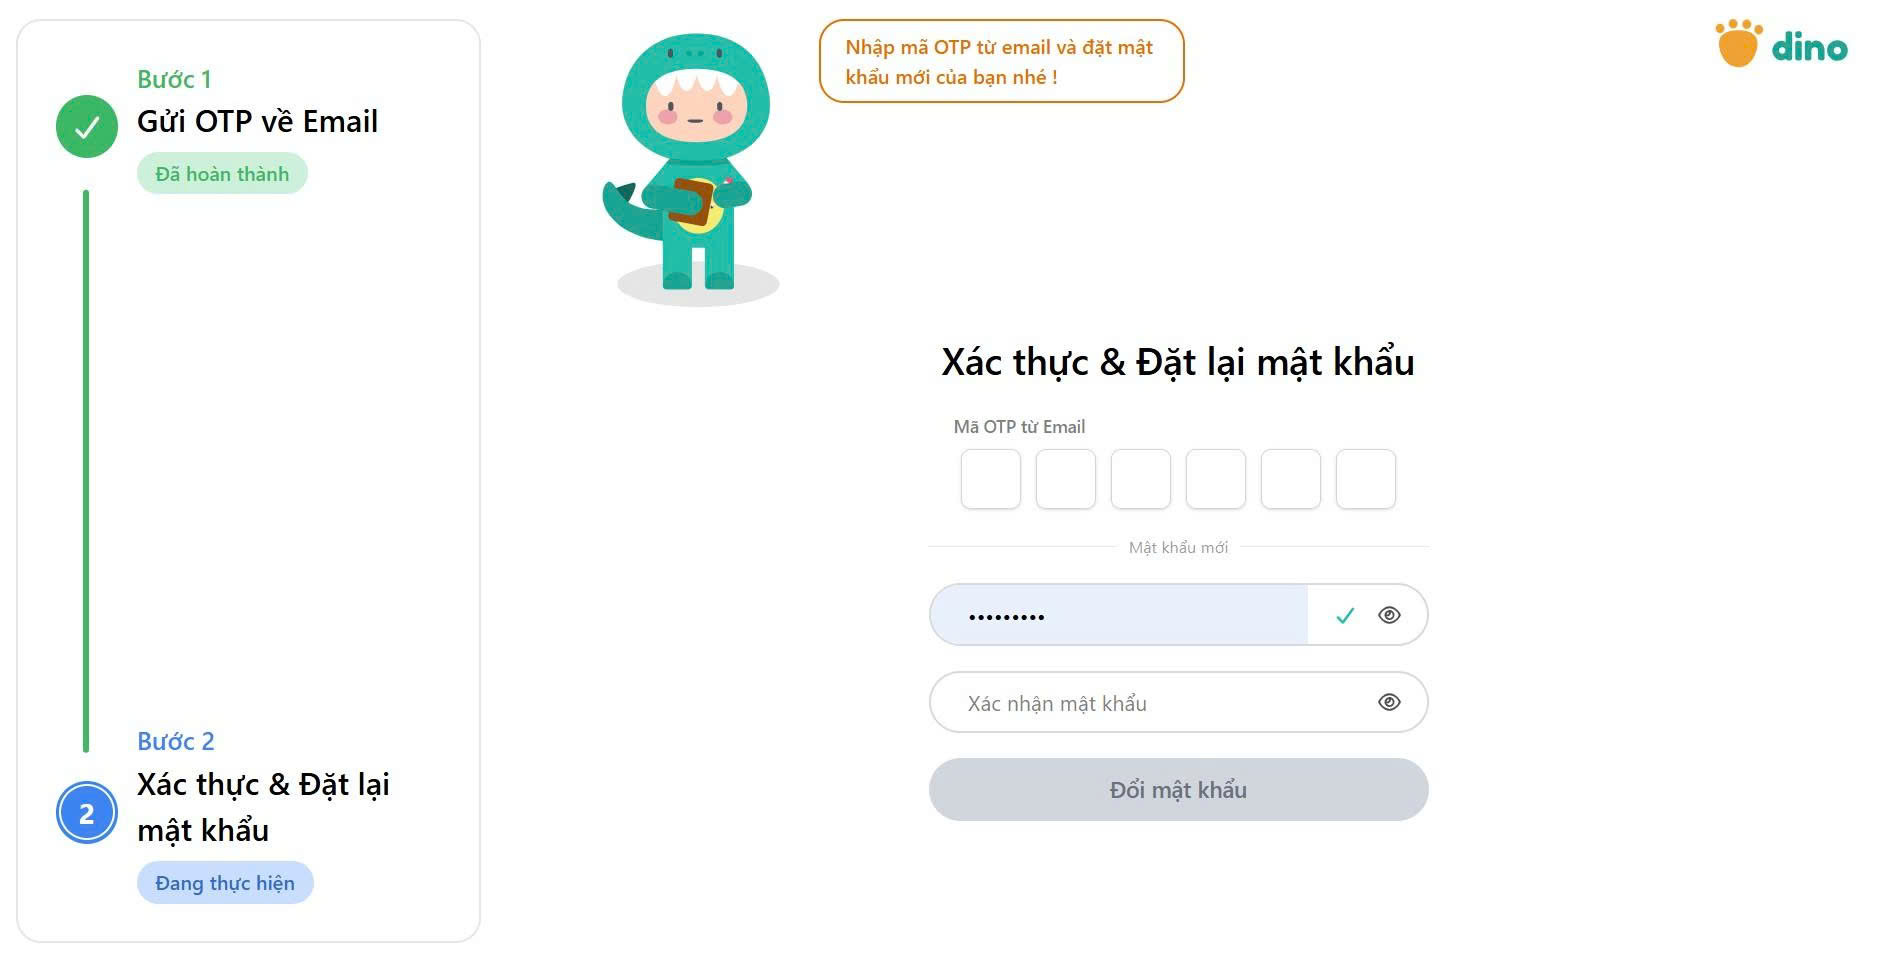
\includegraphics[width=0.9\textwidth]{Image/UI/Auth/PasswordReset2.jpg}
			\vspace{0.6cm}
			\caption{Giao diện Lấy lại mật khẩu - Bước 2}
			\label{fig:inputotp}
		\end{figure}
		
		\item Sau khi đổi mật khẩu thành công, người dùng sẽ nhận được thông báo và được điều hướng về \textbf{Trang đăng nhập} được mô tả ở mục \ref{subsubsec:login}.
	\end{itemize}
\end{{itemize}

\subsection{Các màn hình chính của tài khoản Học sinh}
\textbf{Mô tả tổng quan}
Layout chính của giao diện bao gồm 2 phần: 
\begin{itemize}
	\item \textbf{Thanh điều hướng:} Nằm trên cùng chứa logo thương hiệu của website, các nút điều hướng, nút mở hồ sơ cá nhân, nút thông báo vào nút đăng xuất. Các nút điều hướng tương ứng với từng trang tính năng của website, bao gồm:
	\begin{itemize}
		\item Trang chủ (Nhà)
		\item Trang Bài học
		\item Trang Đấu trường
		\item Trang Bảng xếp hạng
		\item Trang Nhiệm vụ
		\item Trang Minigames
		\item Trang Lịch sử làm bài
	\end{itemize}
	\item \textbf{Phần nội dung} Chiếm phần còn lại của layout, là nơi thể hiện nội dung của các trang tính năng.
\end{itemize}
Layout tổng thể của các màn hình chức năng chính được minh họa thông qua giao diện trang chủ được thiết kế như hình bên dưới.
\begin{figure}[H]
	\centering
	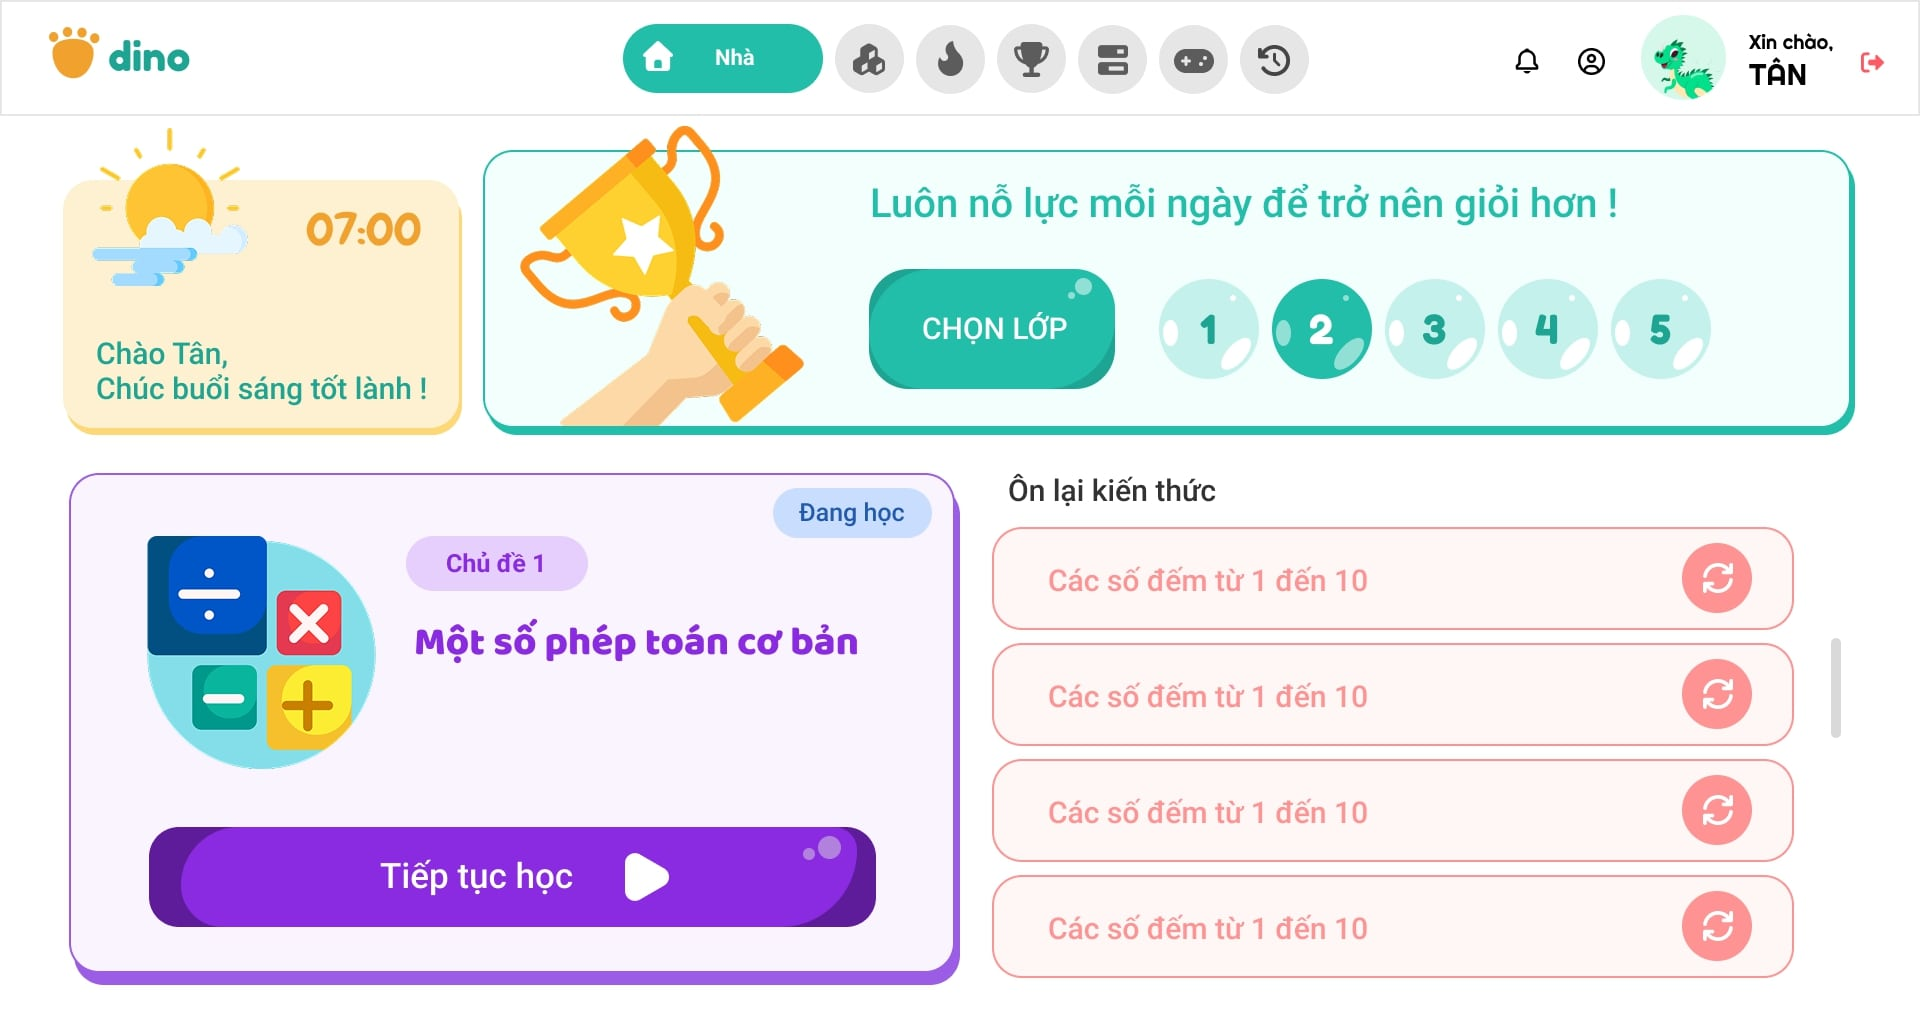
\includegraphics[width=0.9\textwidth]{Image/UI/Main-Student/Home-Morning.jpg}
	\vspace{0.6cm}
	\caption{Trang chủ (minh họa cho layout tổng thể)}
\end{figure}

\subsubsection{Trang chủ}
\label{subsubsec:studenthome}
Trang chủ là trang hiển thị mặc định ngay sau khi học sinh đăng nhập thành công vào hệ thống. Trang chủ có hiển thị giờ giấc và lời chào dành cho người dùng nhằm tạo cảm giác thân thiện và gần gũi. Các thẻ hiển thị giờ và lời chào sẽ thay đổi kiểu thiết kế tùy thuộc vào thời gian trong ngày (Sáng, Chiều, Tối). Giao diện trang chủ vào buổi sáng, buổi chiều và buổi tối được thiết kế lần lượt như các hình \ref{fig:homemorning}, \ref{fig:homeafternoon} và \ref{fig:homenight}. 
\begin{figure}[H]
	\centering
	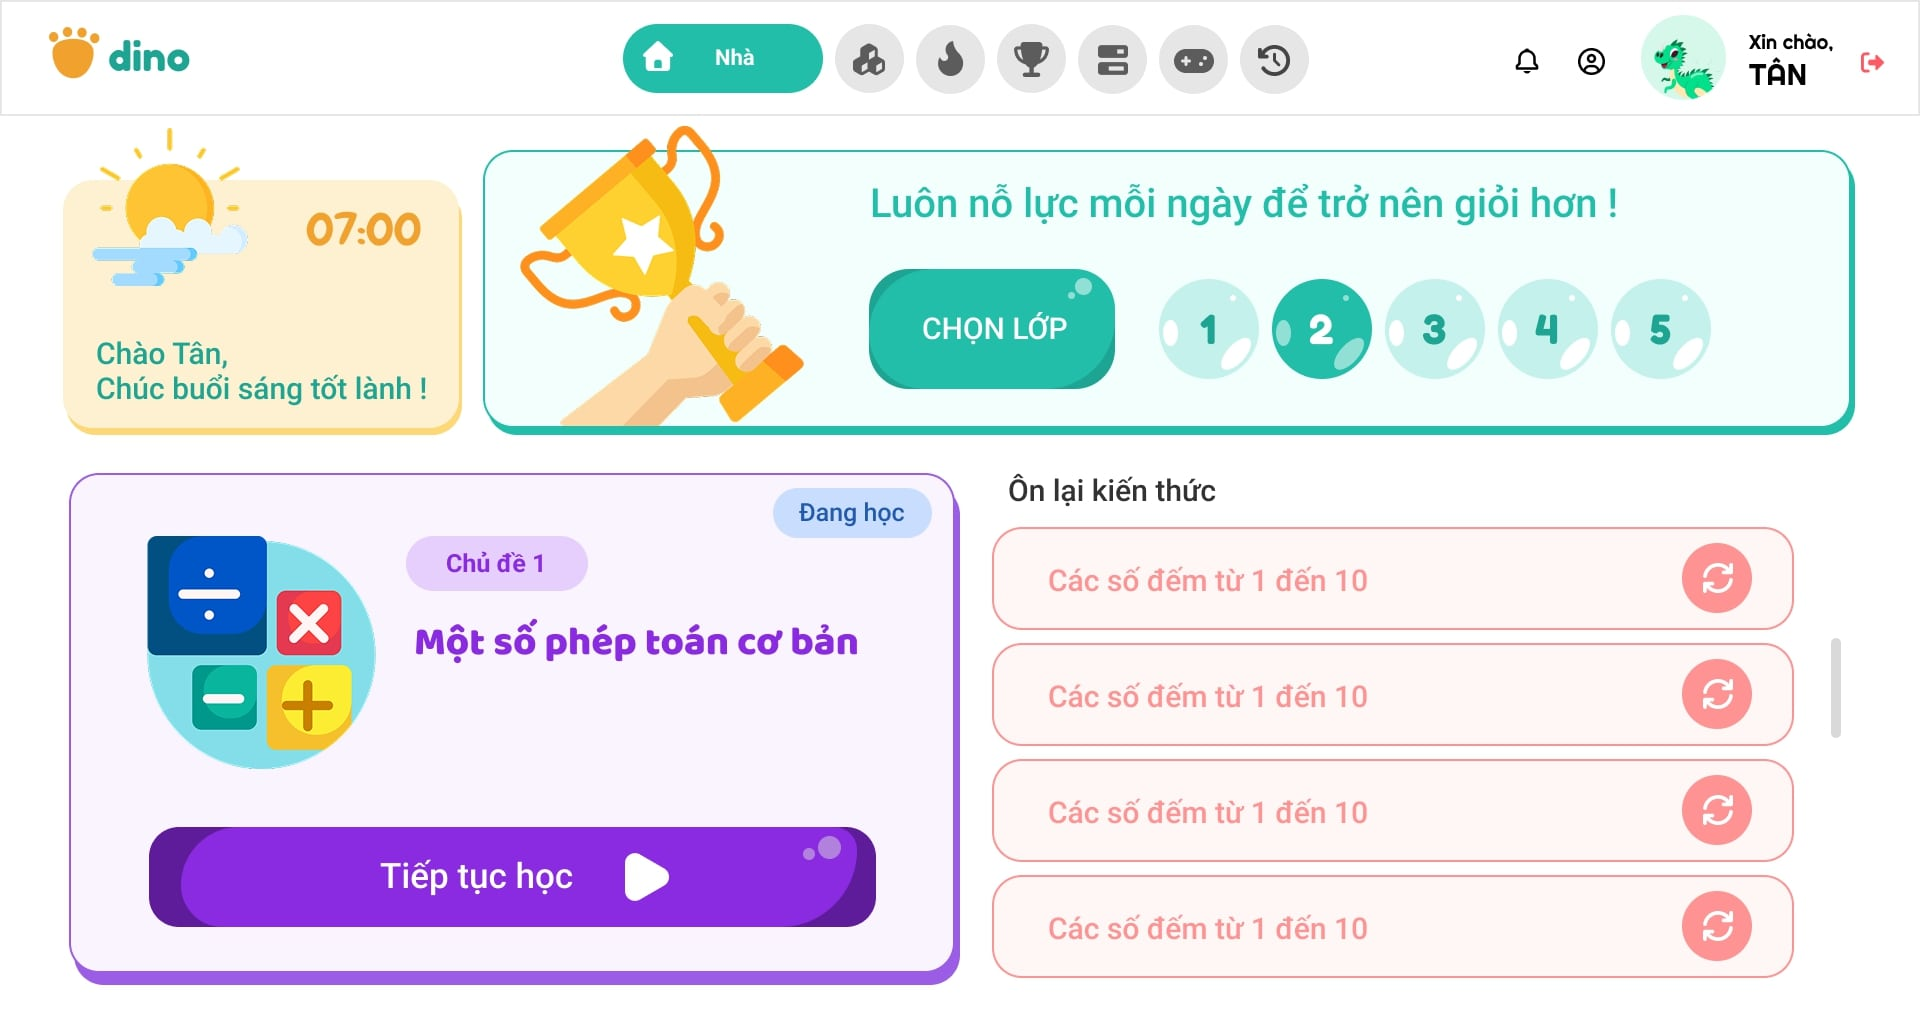
\includegraphics[width=0.9\textwidth]{Image/UI/Main-Student/Home-Morning.jpg}
	\vspace{0.6cm}
	\caption{Trang chủ - Buổi sáng}
	\label{fig:homemorning}
\end{figure}
\begin{figure}[H]
	\centering
	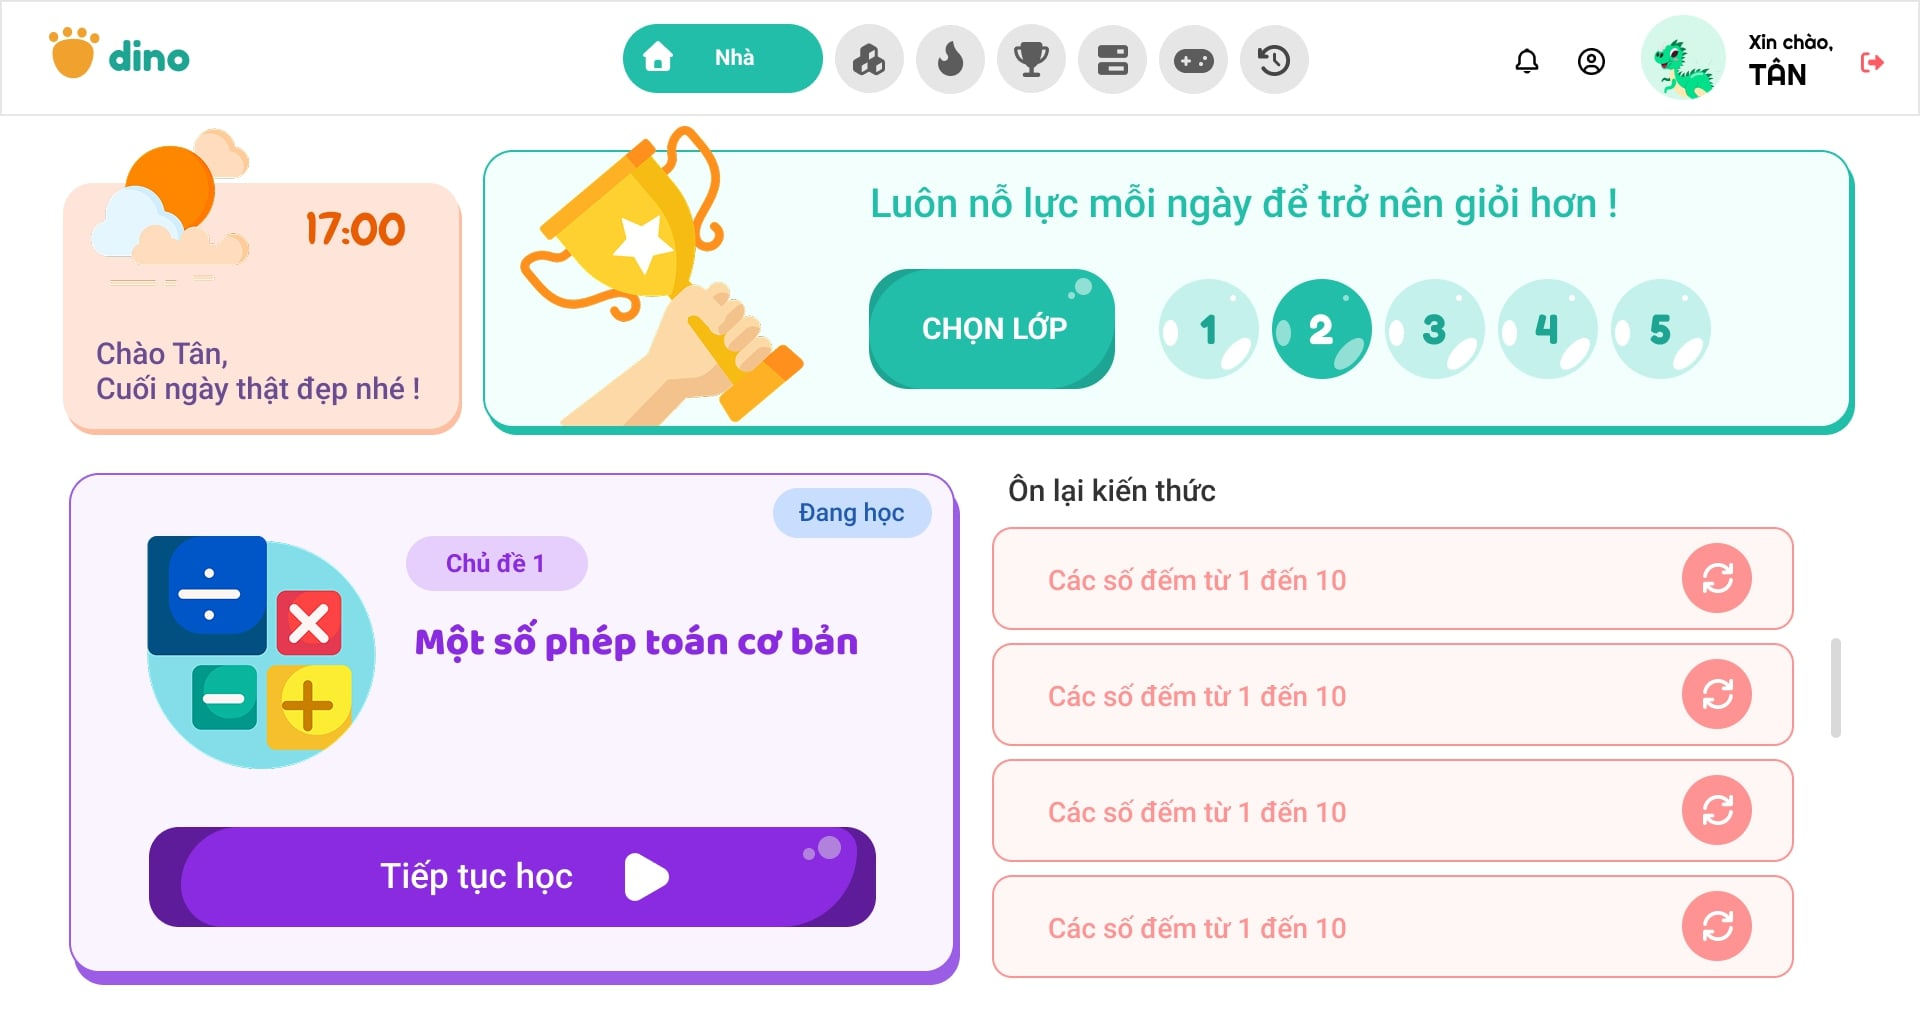
\includegraphics[width=0.9\textwidth]{Image/UI/Main-Student/Home-Afternoon.jpg}
	\vspace{0.6cm}
	\caption{Trang chủ - Buổi chiều}
	\label{fig:homeafternoon}
\end{figure}
\begin{figure}[H]
	\centering
	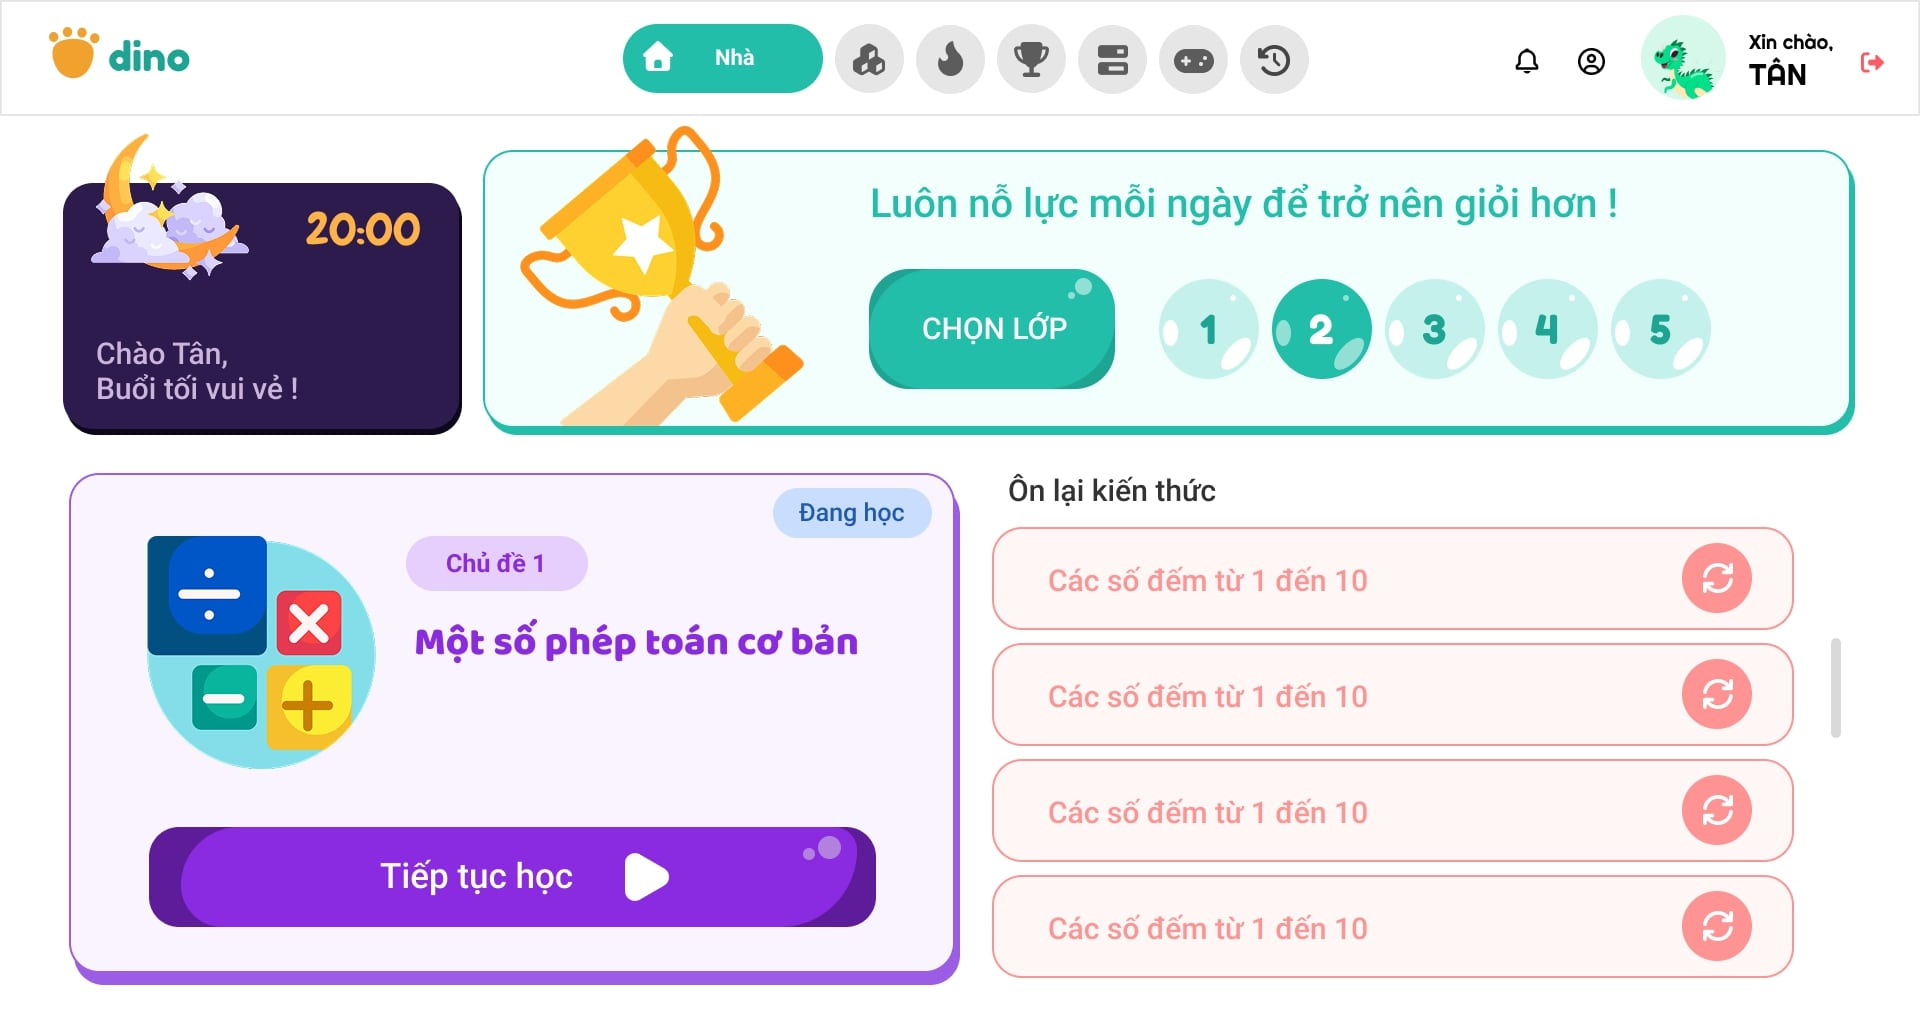
\includegraphics[width=0.9\textwidth]{Image/UI/Main-Student/Home-Night.jpg}
	\vspace{0.6cm}
	\caption{Trang chủ - Buổi tối}
	\label{fig:homenight}
\end{figure}

\vspace{0.2cm}
\newline
Học sinh có thể chọn lớp mình muốn học bằng cách nhấp chuột vào các bong bóng được đánh số từ 1-5. Việc thay đổi lớp ở Trang chủ sẽ không làm thay đổi thông tin về khối lớp trong hồ sơ người dùng.

\vspace{0.2cm}
\newline
Tại trang chủ, hệ thống hiển thị chủ đề gần nhất mà người dùng đã truy cập. Người dùng có thể nhanh chóng quay lại bài học bằng cách nhấn nút \textit{Tiếp tục học}. Bên cạnh đó, các chủ đề đã hoàn thành cũng được liệt kê trong mục \textit{Ôn lại kiến thức} đi kèm với biểu tượng 'Review'. Cả hai thao tác này đều điều hướng người dùng đến cùng một giao diện chi tiết của chủ đề (được mô tả cụ thể tại mục \ref{subsubsec:topic}).

\vspace{0.2cm}
\newpage
Khi người dùng truy cập vào Trang chủ, một thông báo sẽ được hiển thị dưới dạng popup được thiết kế như \textit{Hình \ref{fig:recommend}}. Popup này chứa thông tin gợi ý chủ đề học theo thời gian và khối lớp của người dùng. Người dùng có thể bấm nút \textit{Học ngay} để điều hướng đến trang chủ đề tương ứng được mô tả ở mục \ref{subsubsec:topic}. 
	\begin{figure}[H]
		\centering
		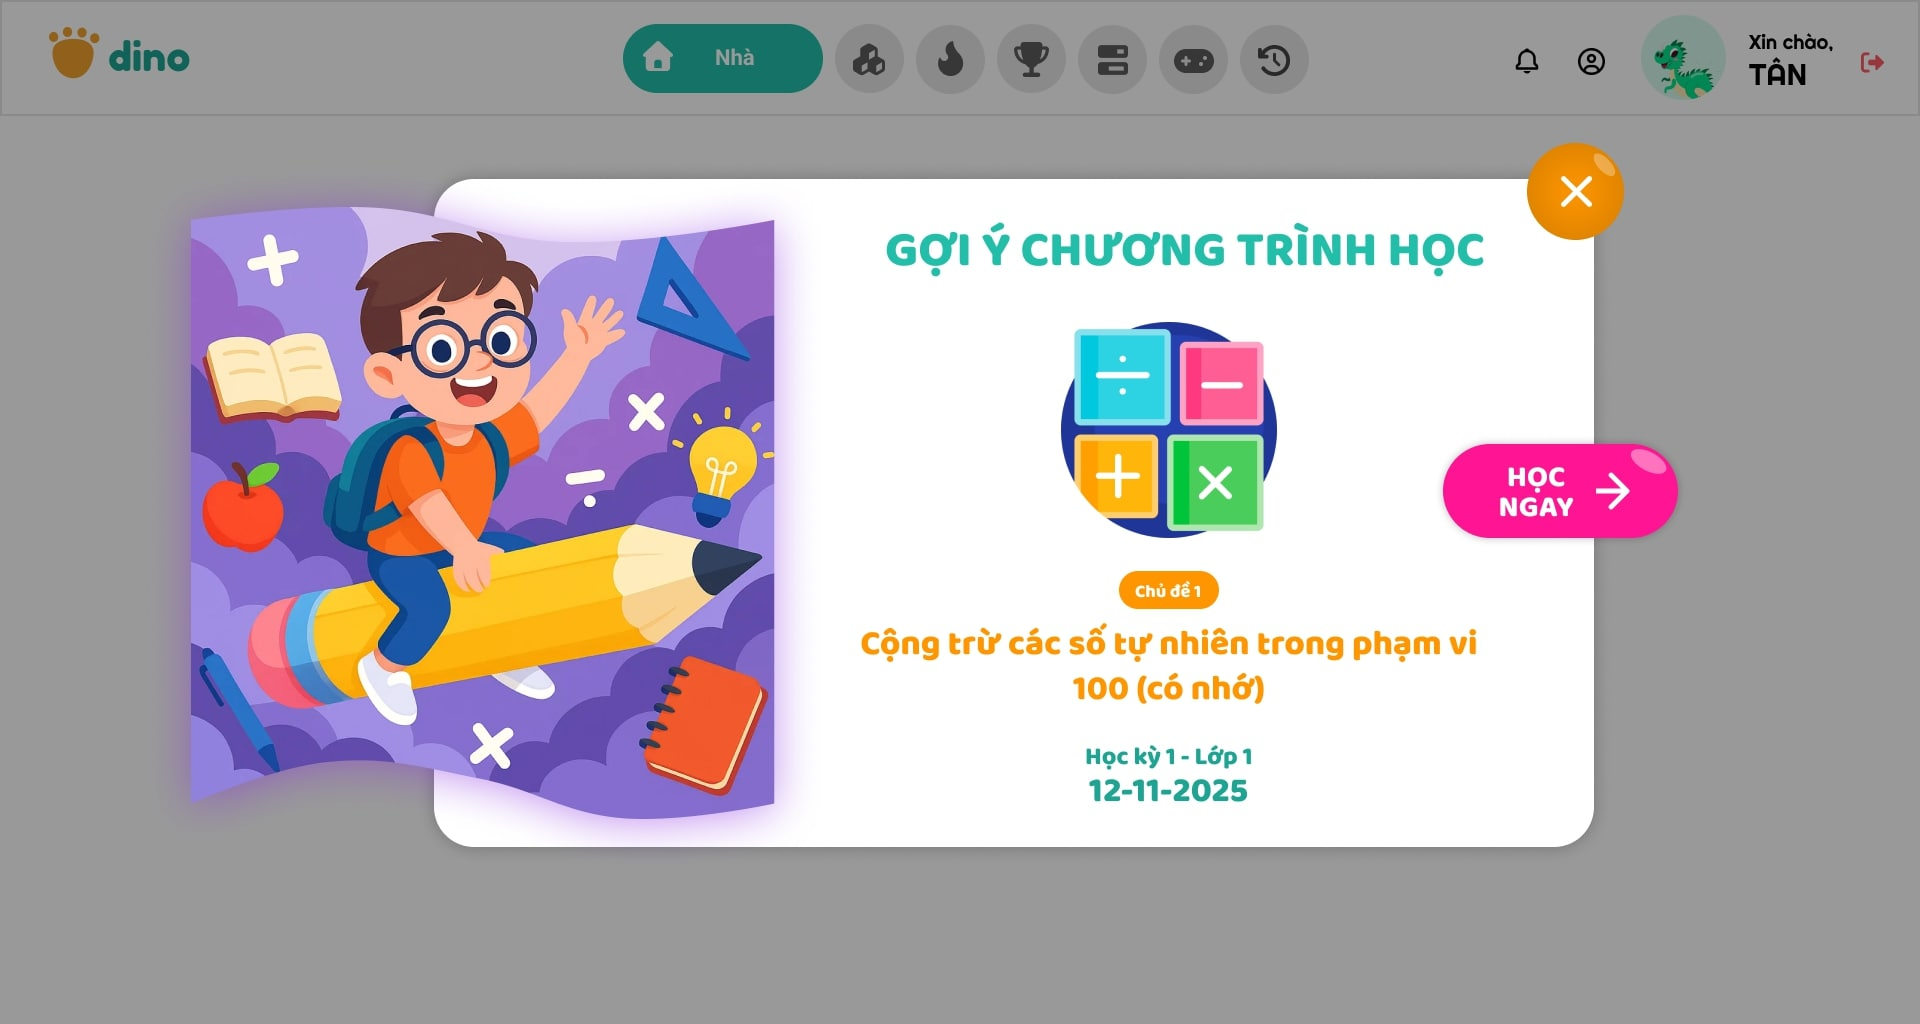
\includegraphics[width=0.9\textwidth]{Image/UI/Main-Student/LessonRecommend.jpg}
		\vspace{0.6cm}
		\caption{Trang chủ - Gợi ý chủ đề học}
		\label{fig:recommend}
	\end{figure}

\vspace{0.2cm}
\newline
Đối với người dùng mới, hệ thống sẽ hiển thị thông báo về bài kiểm tra đầu vào dưới dạng popup được thiết kế như \textit{Hình \ref{fig:enttest}}. Người dùng có thể bấm vào nút \textit{Làm bài} để điều hướng đến giao diện bài kiểm tra được mô tả chi tiết ở mục \ref{subsubsec:exam}, hoặc bấm vào nút \textit{Đóng} để đóng popup. Sau khi đóng, người dùng có thể mở lại popup này bằng cách bấm vào float button hiển thị ở góc phải trên cùng của giao diện trang chủ như \textit{Hình \ref{fig:floatbtn}}.
	\begin{figure}[H]
		\centering
		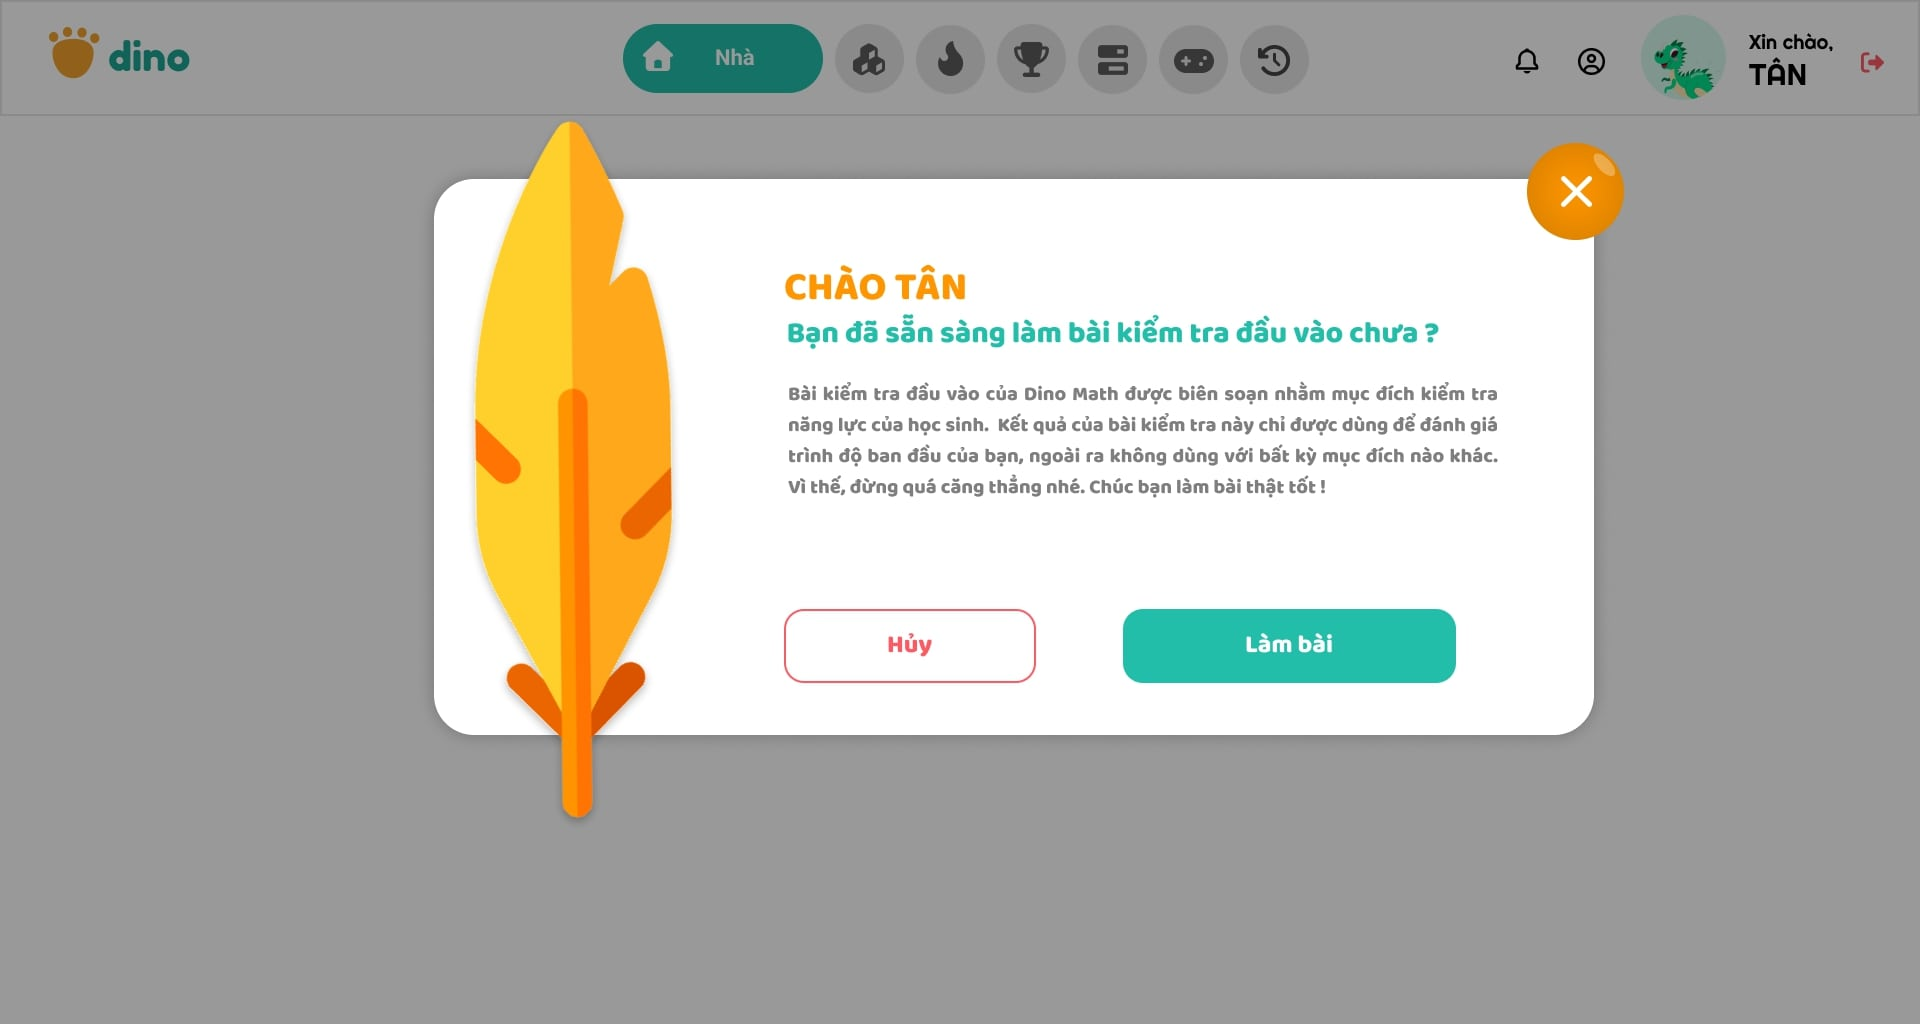
\includegraphics[width=0.9\textwidth]{Image/UI/Main-Student/EntranceTestPopup.jpg}
		\vspace{0.6cm}
		\caption{Trang chủ - Popup thông báo về bài kiểm tra đầu vào}
		\label{fig:enttest}
	\end{figure}
	\begin{figure}[H]
		\centering
		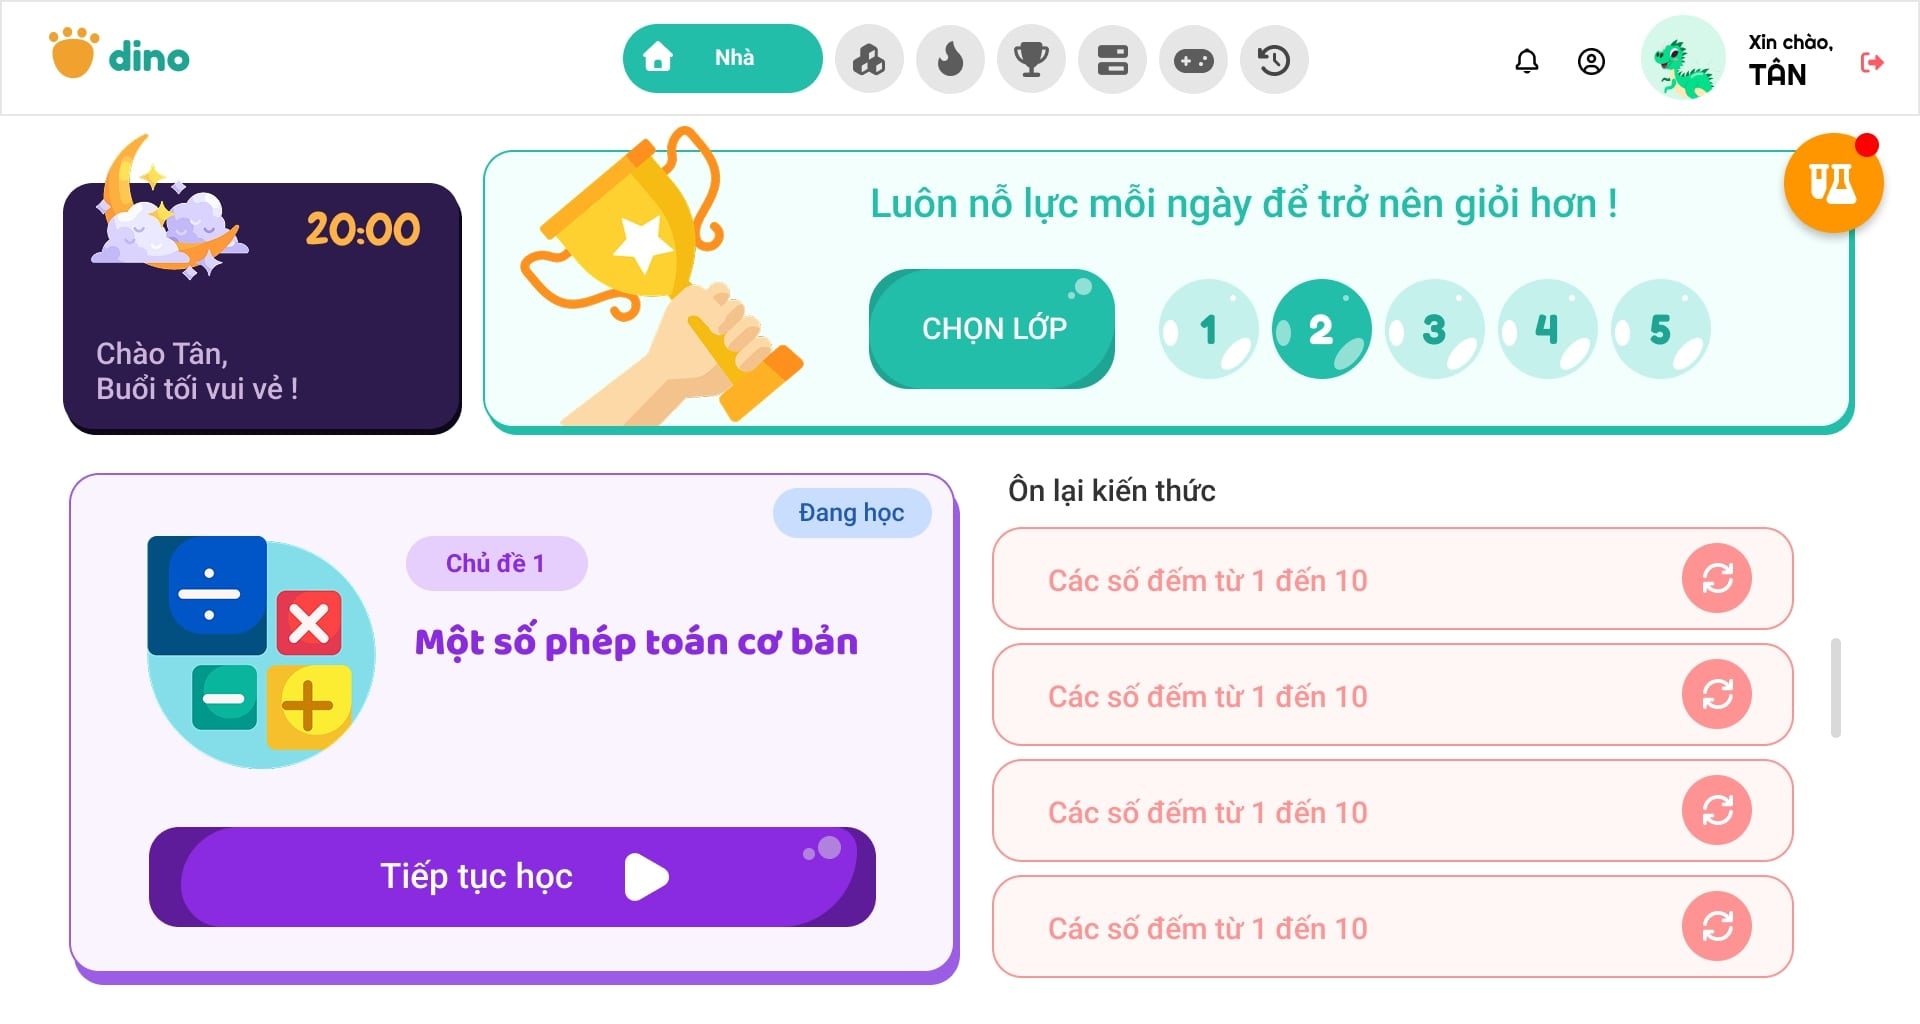
\includegraphics[width=0.9\textwidth]{Image/UI/Main-Student/EntranceTestFloatingButton.jpg}
		\vspace{0.6cm}
		\caption{Trang chủ - Nút mở popup bài kiểm tra đầu vào ở góc trên bên phải}
		\label{fig:floatbtn}
	\end{figure}


\subsubsection{Trang Bài học}
\label{subsubsec:lesson}
Phần nội dung chính của trang Bài học liệt kê danh sách toàn bộ các chủ đề thuộc khối lớp hiện tại, bao gồm cả những chủ đề đã được mở khóa (như minh họa tại \textit{Hình \ref{fig:lesson}}) và các chủ đề còn đang trong trạng thái khóa (như minh họa tại \textit{Hình \ref{fig:lessonlocked}}). Để bắt đầu quá trình học, người dùng có thể nhấn vào các thẻ chủ đề trong danh sách. Bên cạnh đó, người dùng cũng có thể nhanh chóng quay lại nội dung đang học dang dở bằng cách nhấn nút \textit{Bắt đầu} nằm trong container chủ đề được bố trí phía trên danh sách. Cả 2 thao tác kể trên đều sẽ điều hướng người dùng đến \textbf{Trang Chủ đề} được mô tả ở mục \ref{subsubsec:topic}.

\begin{figure}[H]
	\centering
	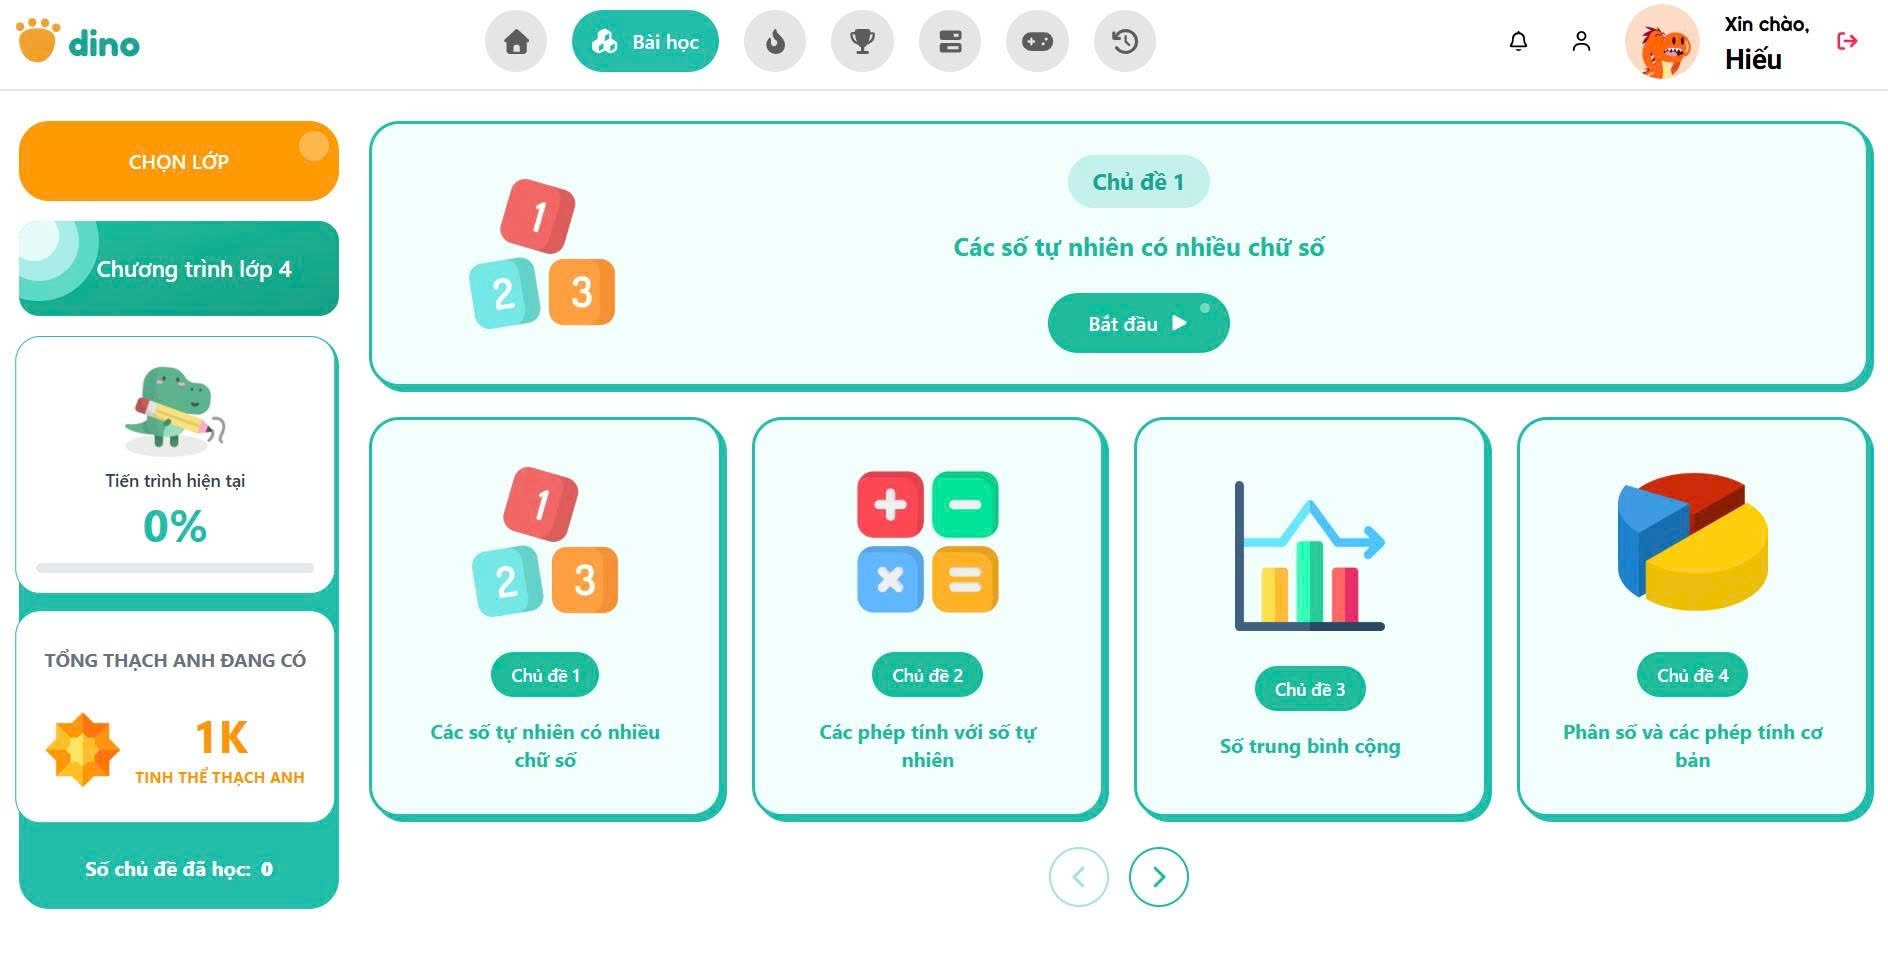
\includegraphics[width=0.9\textwidth]{Image/UI/Main-Student/Topics-G4.jpg}
	\vspace{0.6cm}
	\caption{Trang Bài học - Các chủ đề của Lớp 4 (tương tự với các lớp khác)}
	\label{fig:lesson}
\end{figure}
\begin{figure}[H]
	\centering
	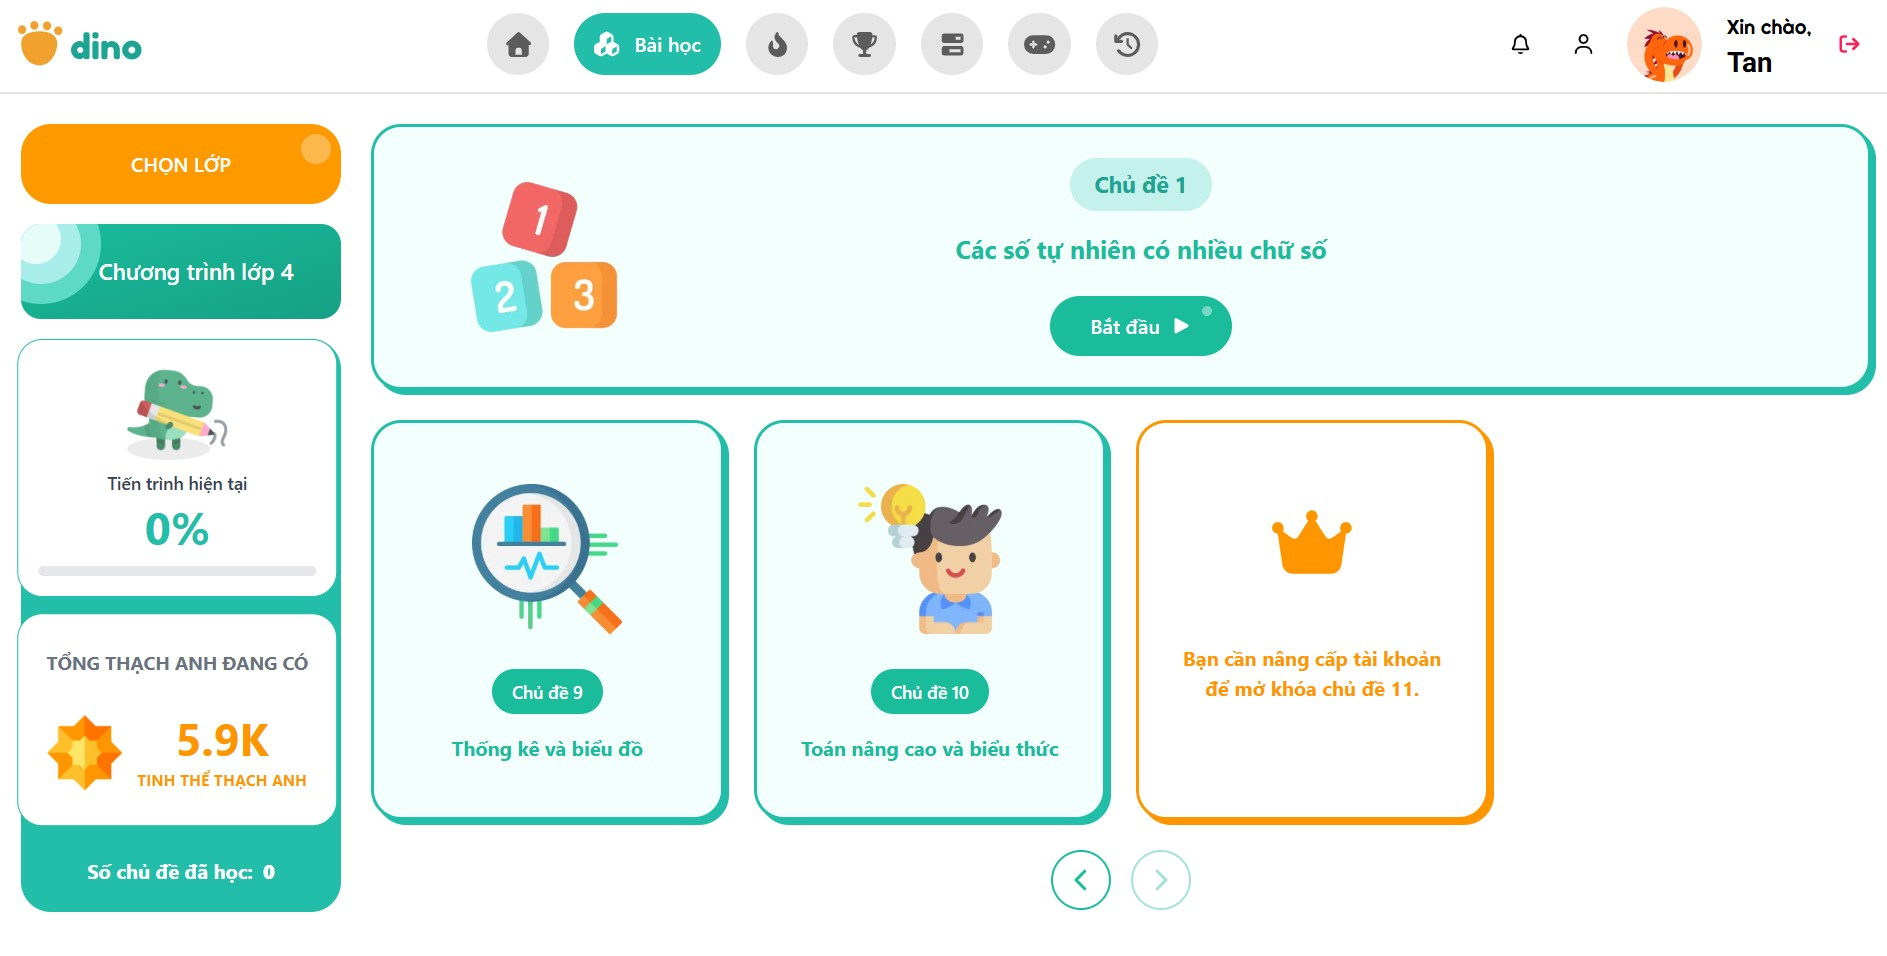
\includegraphics[width=0.9\textwidth]{Image/UI/Main-Student/PremiumTopic.jpg}
	\vspace{0.6cm}
	\caption{Trang Bài học - Các chủ đề bị khóa}
	\label{fig:lessonlocked}
\end{figure}

\vspace{0.2cm}
\newline
Ngoài liệt kê danh sách các bài học, hệ thống còn hiển thị rõ ràng thông tin về khối lớp hiện tại mà học sinh đã lựa chọn ở \textbf{Trang chủ} (được mô tả chi tiết trong mục \ref{subsubsec:studenthome}). Đi kèm với đó, hệ thống sẽ cập nhật tiến trình học tập hiện tại thông qua tỉ lệ phần trăm các chủ đề đã hoàn thành trên tổng số chủ đề thuộc khối lớp đó. Ngoài ra, tổng số lượng Thạch anh tích lũy được từ các hoạt động học tập cũng được hiển thị đầy đủ, đóng vai trò như một hệ thống điểm thưởng để xếp hạng người dùng. Hệ thống cũng cung cấp các số liệu thống kê cụ thể bao gồm số lượng chủ đề đã học, số lượng chủ đề đã mở khóa và thông tin về chủ đề gần nhất mà người dùng vừa truy cập.

\subsubsection{Trang Chủ đề (Trang Milestones)}
\label{subsubsec:topic}
\textbf{Trang Chủ đề} chỉ có thể truy cập bằng cách bấm vào các thẻ chủ đề ở \textbf{Trang Bài học} trong mục \ref{subsubsec:lesson} hoặc bấm vào các nút \textit{Tiếp tục học/Bắt đầu} trong container hiển thị chủ đề học gần nhất được mô tả ở \textbf{Trang chủ} (mục \ref{subsubsec:studenthome}) và \textbf{Trang Bài học} (mục \ref{subsubsec:lesson}). Nhóm thiết kế giao diện cho \textbf{Trang Chủ đề} theo phong cách phiêu lưu qua từng thế giới và vùng đất, tạo cho người dùng cảm giác hứng thú với việc học tập. Mỗi khối lớp gắn liền với một thế giới khác nhau, mỗi thế giới lại gồm các vùng đất khác nhau ứng với các độ khó khác nhau. Trang còn bao gồm danh sách các milestone, mỗi milestone đóng vai trò như một bài học trong chủ đề bao gồm nhiều bài tập tương tác giúp học sinh luyện tập khả năng làm toán.

\vspace{0.2cm}
\newline
Ngoài ra, trang còn hiển thị tên chủ đề hiện tại cùng với tiến trình học tập (tỉ lệ phần trăm các milestone đã học trên tổng số milestone của chủ đề đó). Người dùng phải học hết các milestone thuộc một độ khó nhất định thì mới mở khóa được các milestone ở độ khó tiếp theo. Người dùng có thể bấm vào nút mũi tên ở 2 bên chuyển đổi giữa các milestone, sau đó bấm nút \textit{Làm bài nào !} để điều hướng sang \textbf{Trang Bài tập} được mô tả ở mục \ref{subsubsec:exercise}. 

\newpage
	% --- Trang Chủ đề của Lớp 1 ---
	\noindent Thế giới của Lớp 1 được thiết kế với bối cảnh thảo nguyên do đây là lớp nhỏ nhất và có độ khó thấp nhất. Các hình từ \ref{fig:e1} đến \ref{fig:h1} là thiết kế cho trang chủ đề của lớp 1 ứng với các mức độ khó khác nhau của bài học. Giao diện khóa của các bài học (milestone) được thiết kế như \textit{Hình \ref{fig:l1}}.
	\begin{figure}[H]
		\centering
		\begin{minipage}{0.45\textwidth}
			\centering
			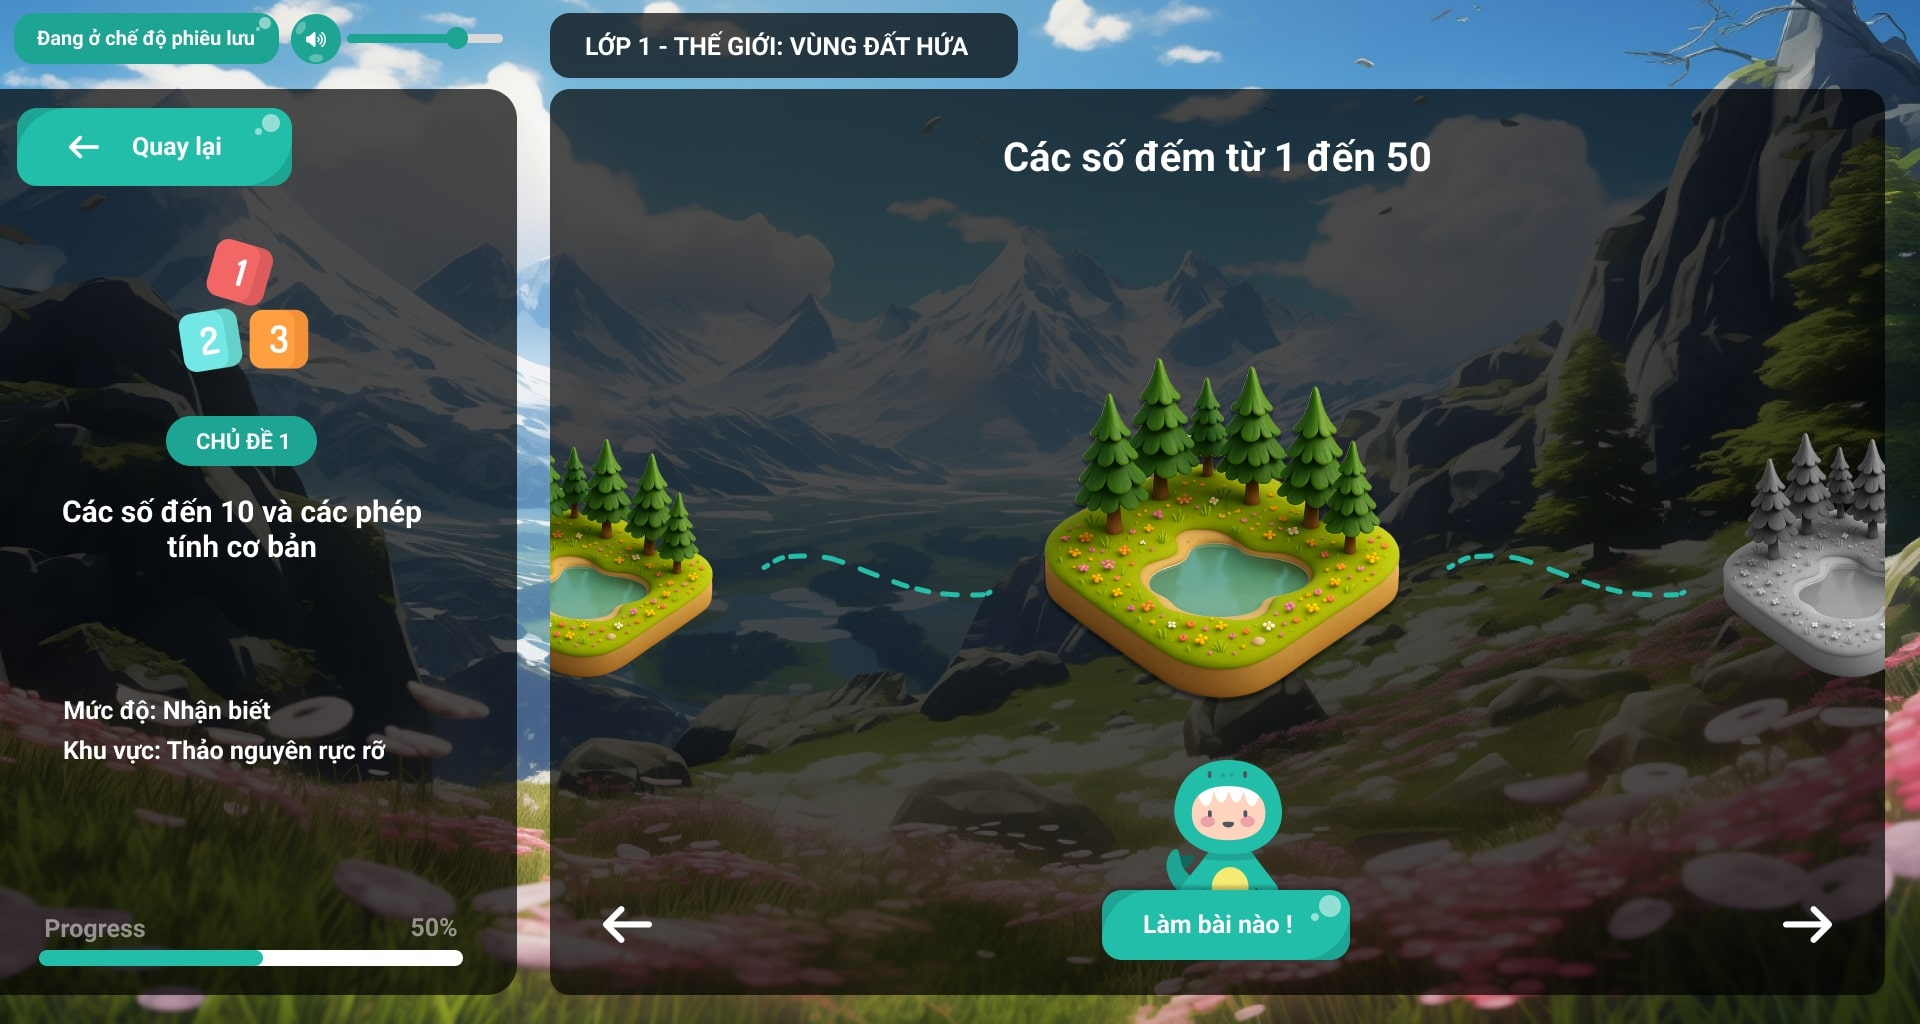
\includegraphics[width=\textwidth]{Image/UI/Milestones/Paths-G1-NB.jpg}
			\vspace{0.2cm}
			\caption{Lớp 1 - Nhận biết}
			\label{fig:e1}
		\end{minipage}
		\hspace{0.1cm}
		\begin{minipage}{0.45\textwidth}
			\centering
			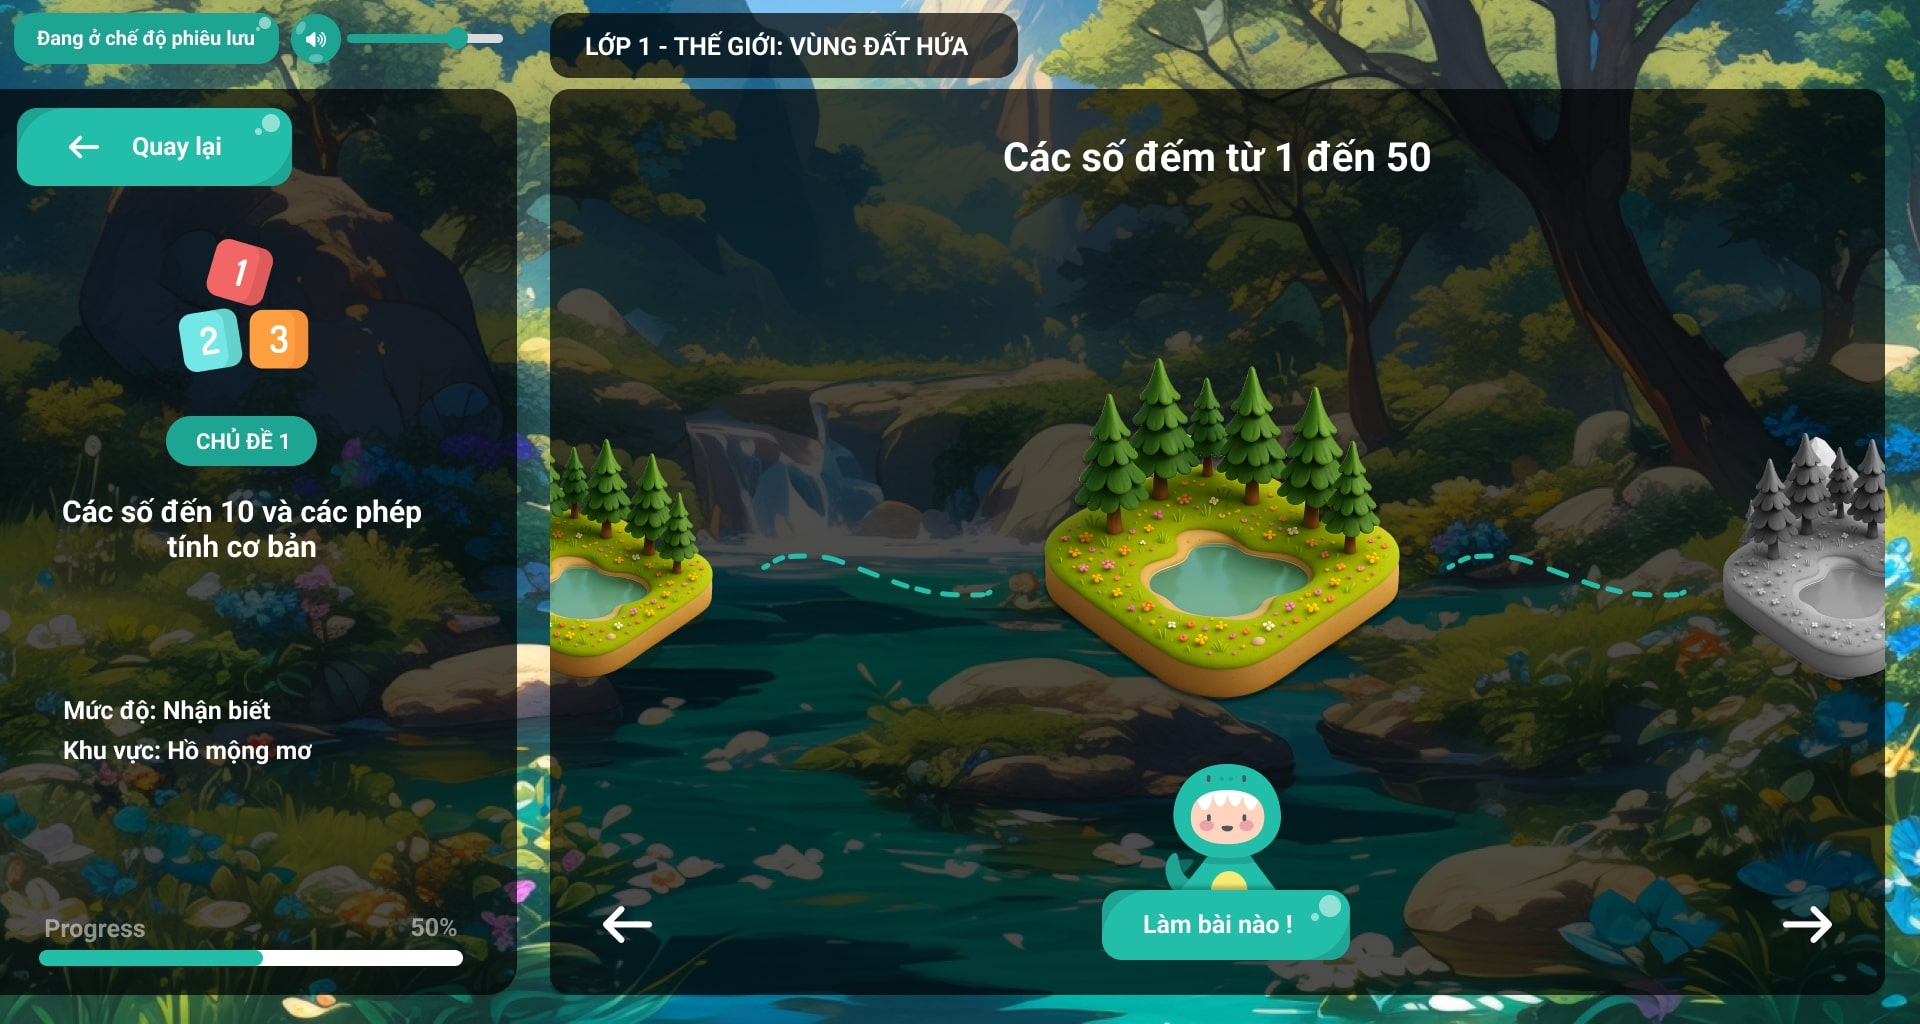
\includegraphics[width=\textwidth]{Image/UI/Milestones/Paths-G1-TH.jpg}
			\vspace{0.2cm}
			\caption{Lớp 1 - Thông hiểu}
			\label{fig:md1}
		\end{minipage}
		
		\vspace{0.4cm}
		
		\begin{minipage}{0.45\textwidth}
			\centering
			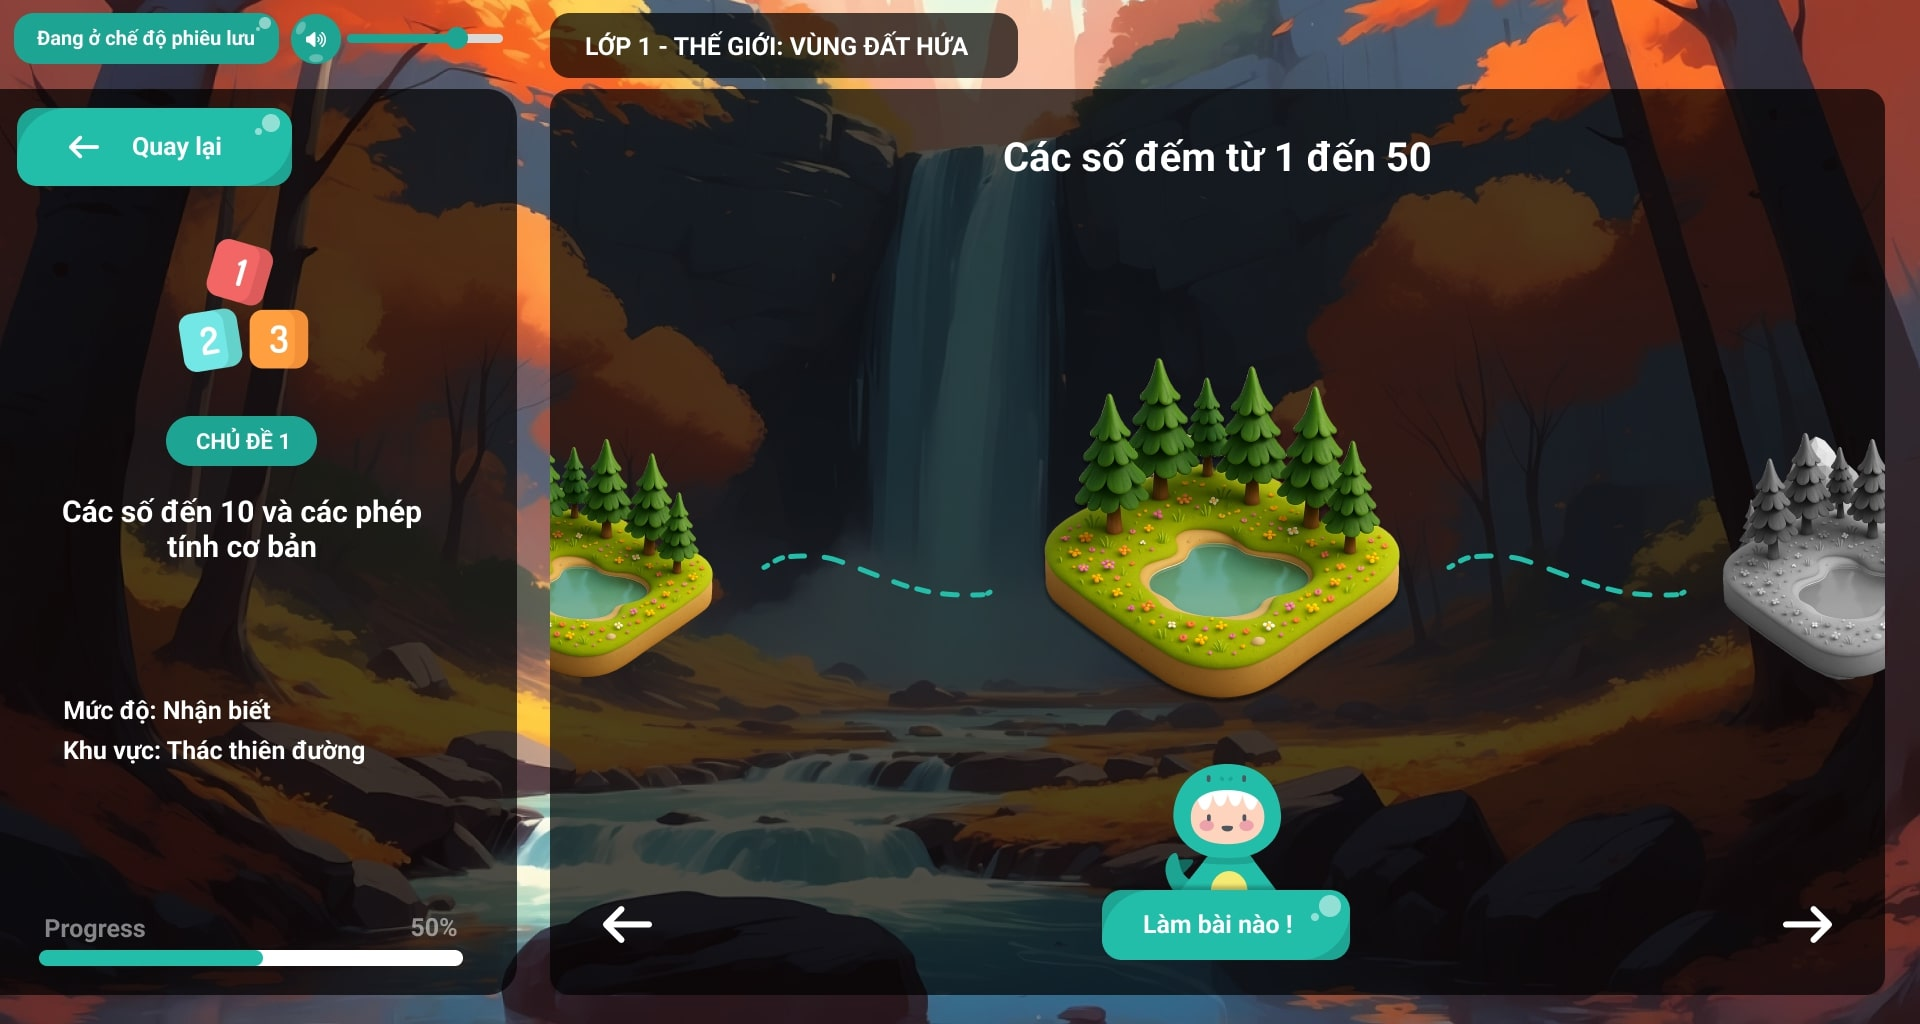
\includegraphics[width=\textwidth]{Image/UI/Milestones/Paths-G1-VD.jpg}
			\vspace{0.2cm}
			\caption{Lớp 1 - Vận dụng}
			\label{fig:h1}
		\end{minipage}
		\hspace{0.1cm}
		\begin{minipage}{0.45\textwidth}
			\centering
			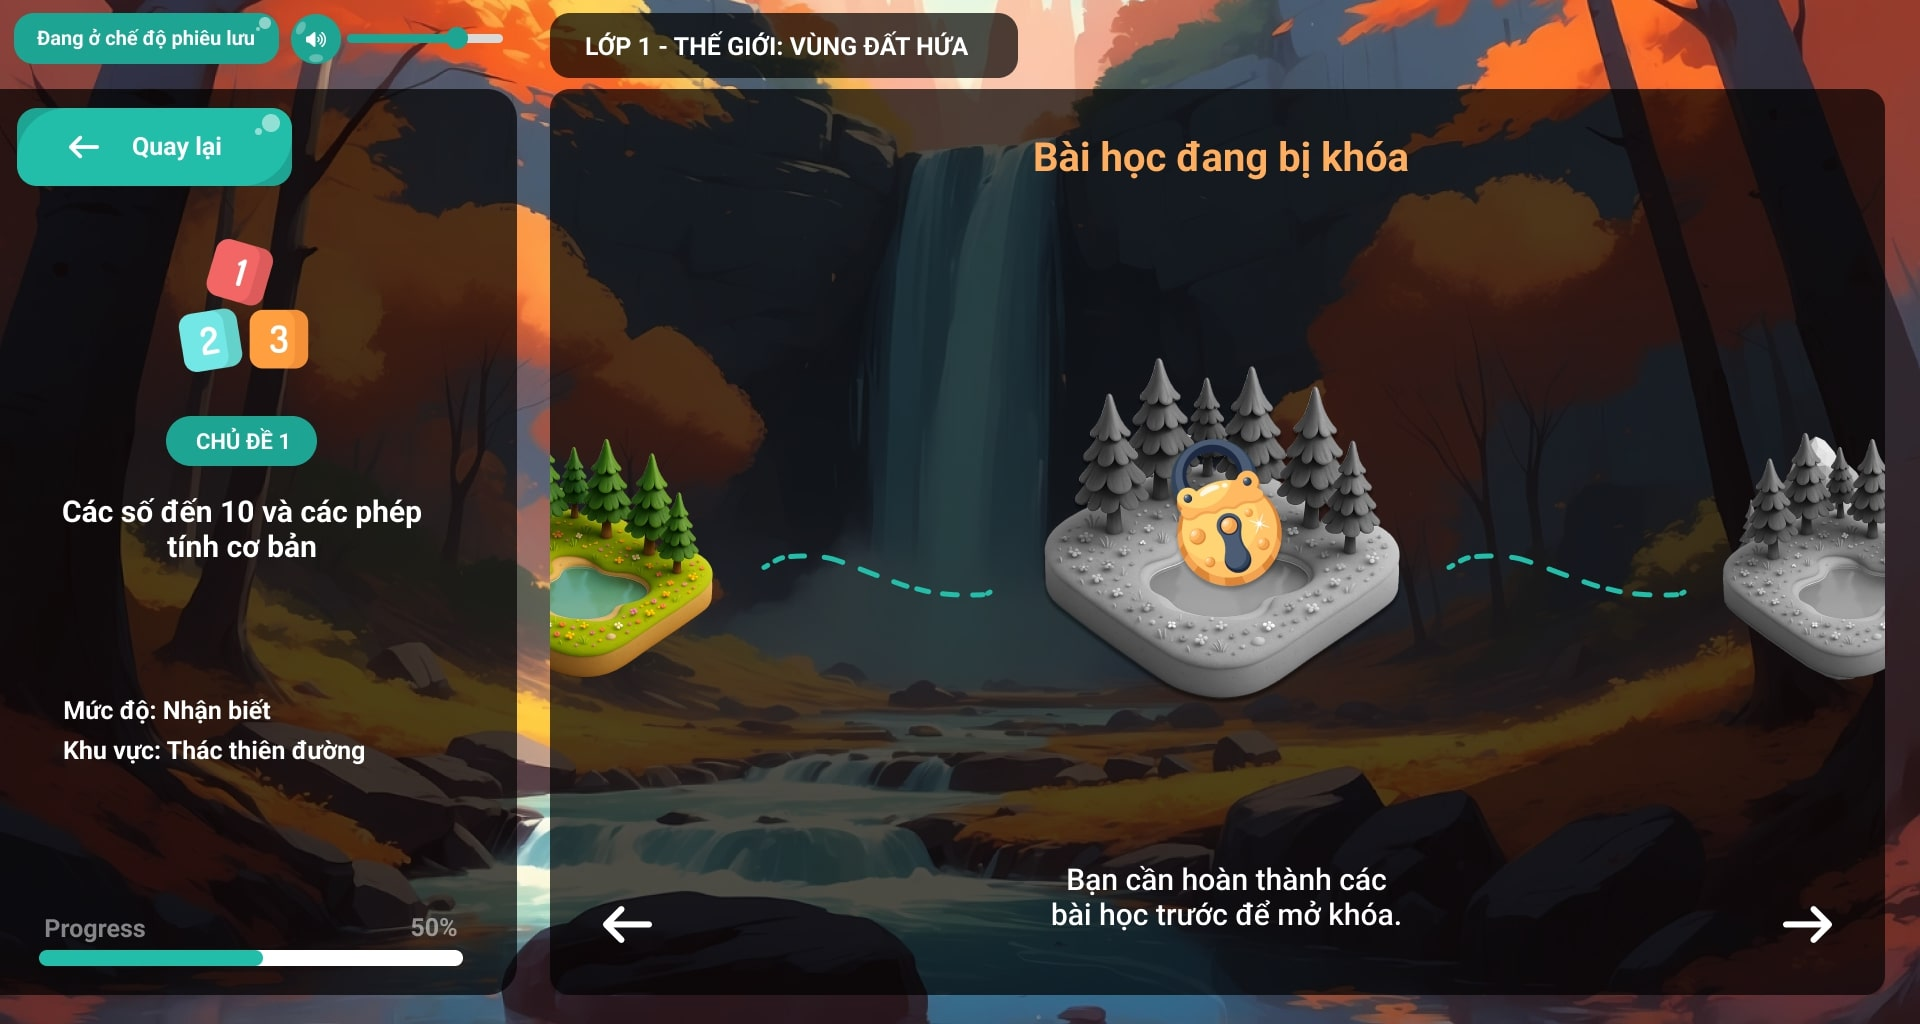
\includegraphics[width=\textwidth]{Image/UI/Milestones/Paths-G1-Locked.jpg}
			\vspace{0.2cm}
			\caption{Lớp 1 - Milestone bị khóa}
			\label{fig:l1}
		\end{minipage}
	\end{figure}
	
	\vspace{0.4cm}
	
	% --- Trang Chủ đề của Lớp 2 ---
	\noindent Thế giới của Lớp 2 được thiết kế với bối cảnh rừng rậm, khắc nghiệt hơn thảo nguyên một chút. Các hình từ \ref{fig:e2} đến \ref{fig:h2} là thiết kế cho trang chủ đề của lớp 2 ứng với các mức độ khó khác nhau của bài học. Giao diện khóa của các bài học (milestone) được thiết kế như \textit{Hình \ref{fig:l2}}.
	\begin{figure}[H]
		\centering
		\begin{minipage}{0.45\textwidth}
			\centering
			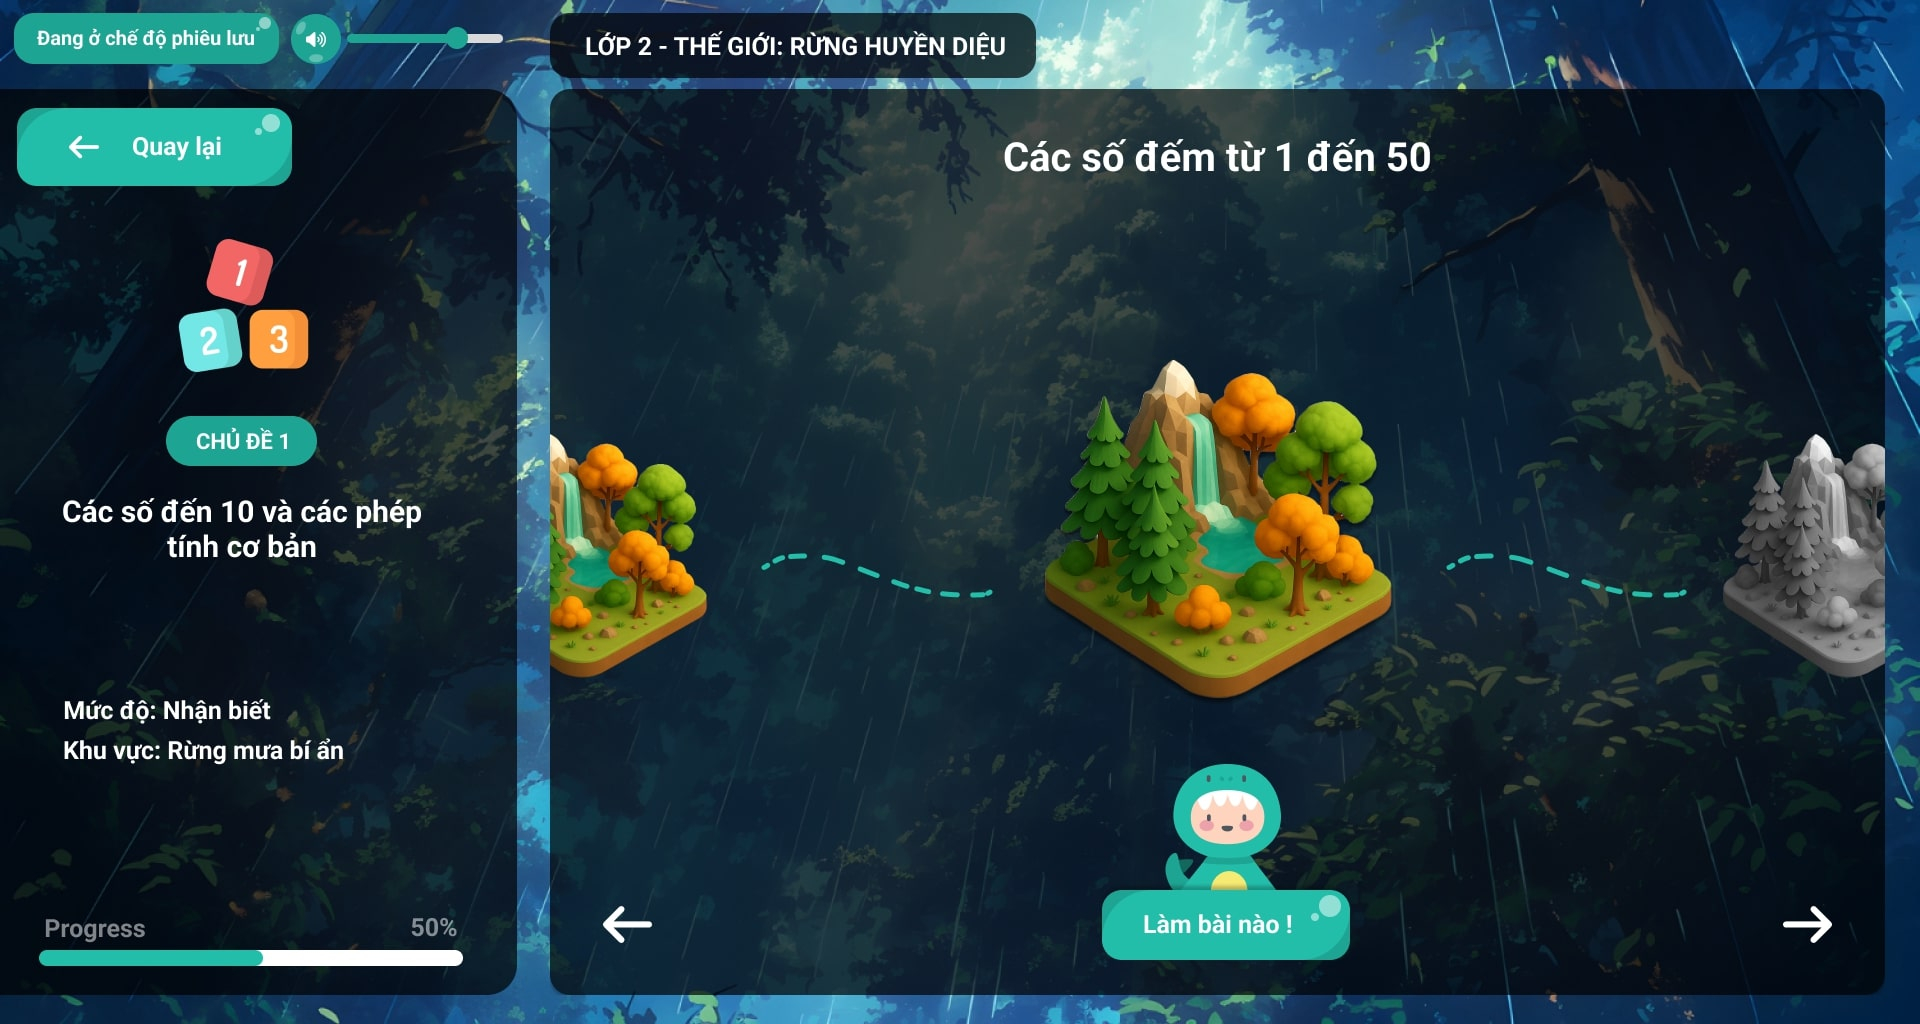
\includegraphics[width=\textwidth]{Image/UI/Milestones/Paths-G2-NB.jpg}
			\vspace{0.2cm}
			\caption{Lớp 2 - Nhận biết}
			\label{fig:e2}
		\end{minipage}
		\hspace{0.1cm}
		\begin{minipage}{0.45\textwidth}
			\centering
			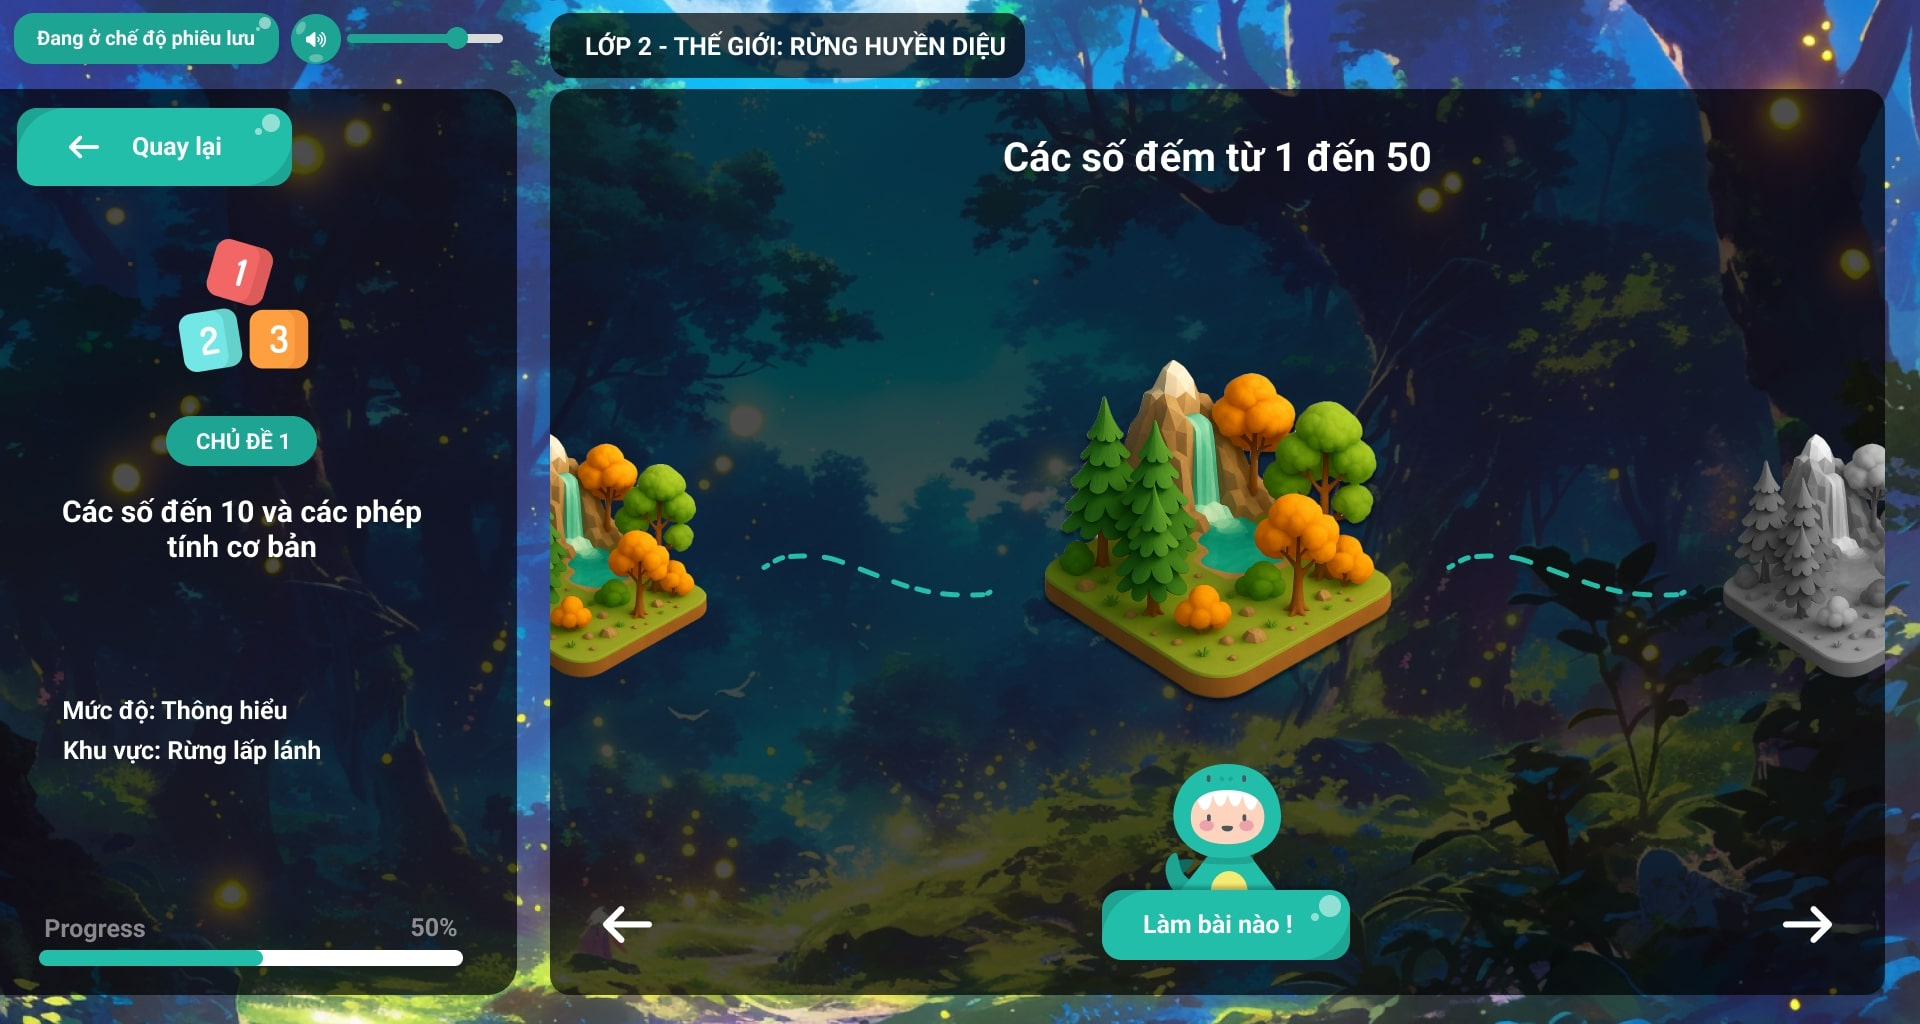
\includegraphics[width=\textwidth]{Image/UI/Milestones/Paths-G2-TH.jpg}
			\vspace{0.2cm}
			\caption{Lớp 2 - Thông hiểu}
			\label{fig:md2}
		\end{minipage}
		
		\vspace{0.4cm}
		
		\begin{minipage}{0.45\textwidth}
			\centering
			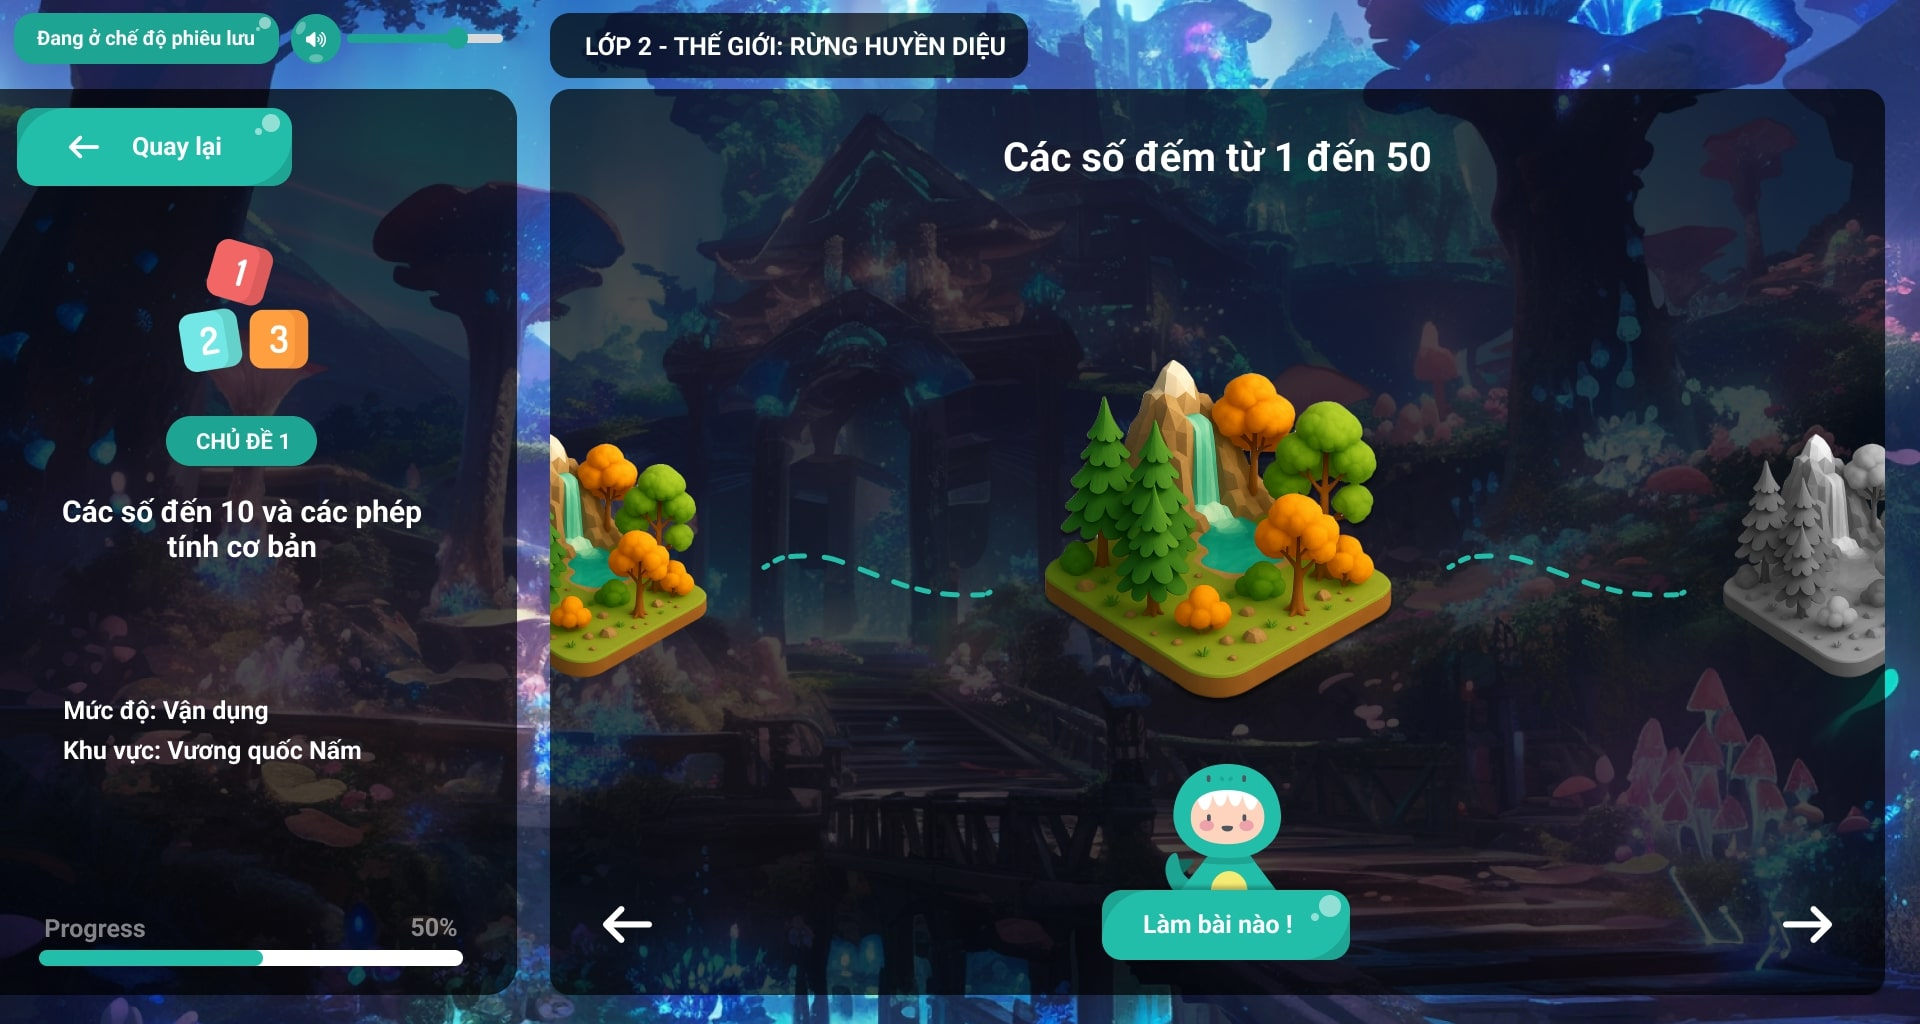
\includegraphics[width=\textwidth]{Image/UI/Milestones/Paths-G2-VD.jpg}
			\vspace{0.2cm}
			\caption{Lớp 2 - Vận dụng}
			\label{fig:h2}
		\end{minipage}
		\hspace{0.1cm}
		\begin{minipage}{0.45\textwidth}
			\centering
			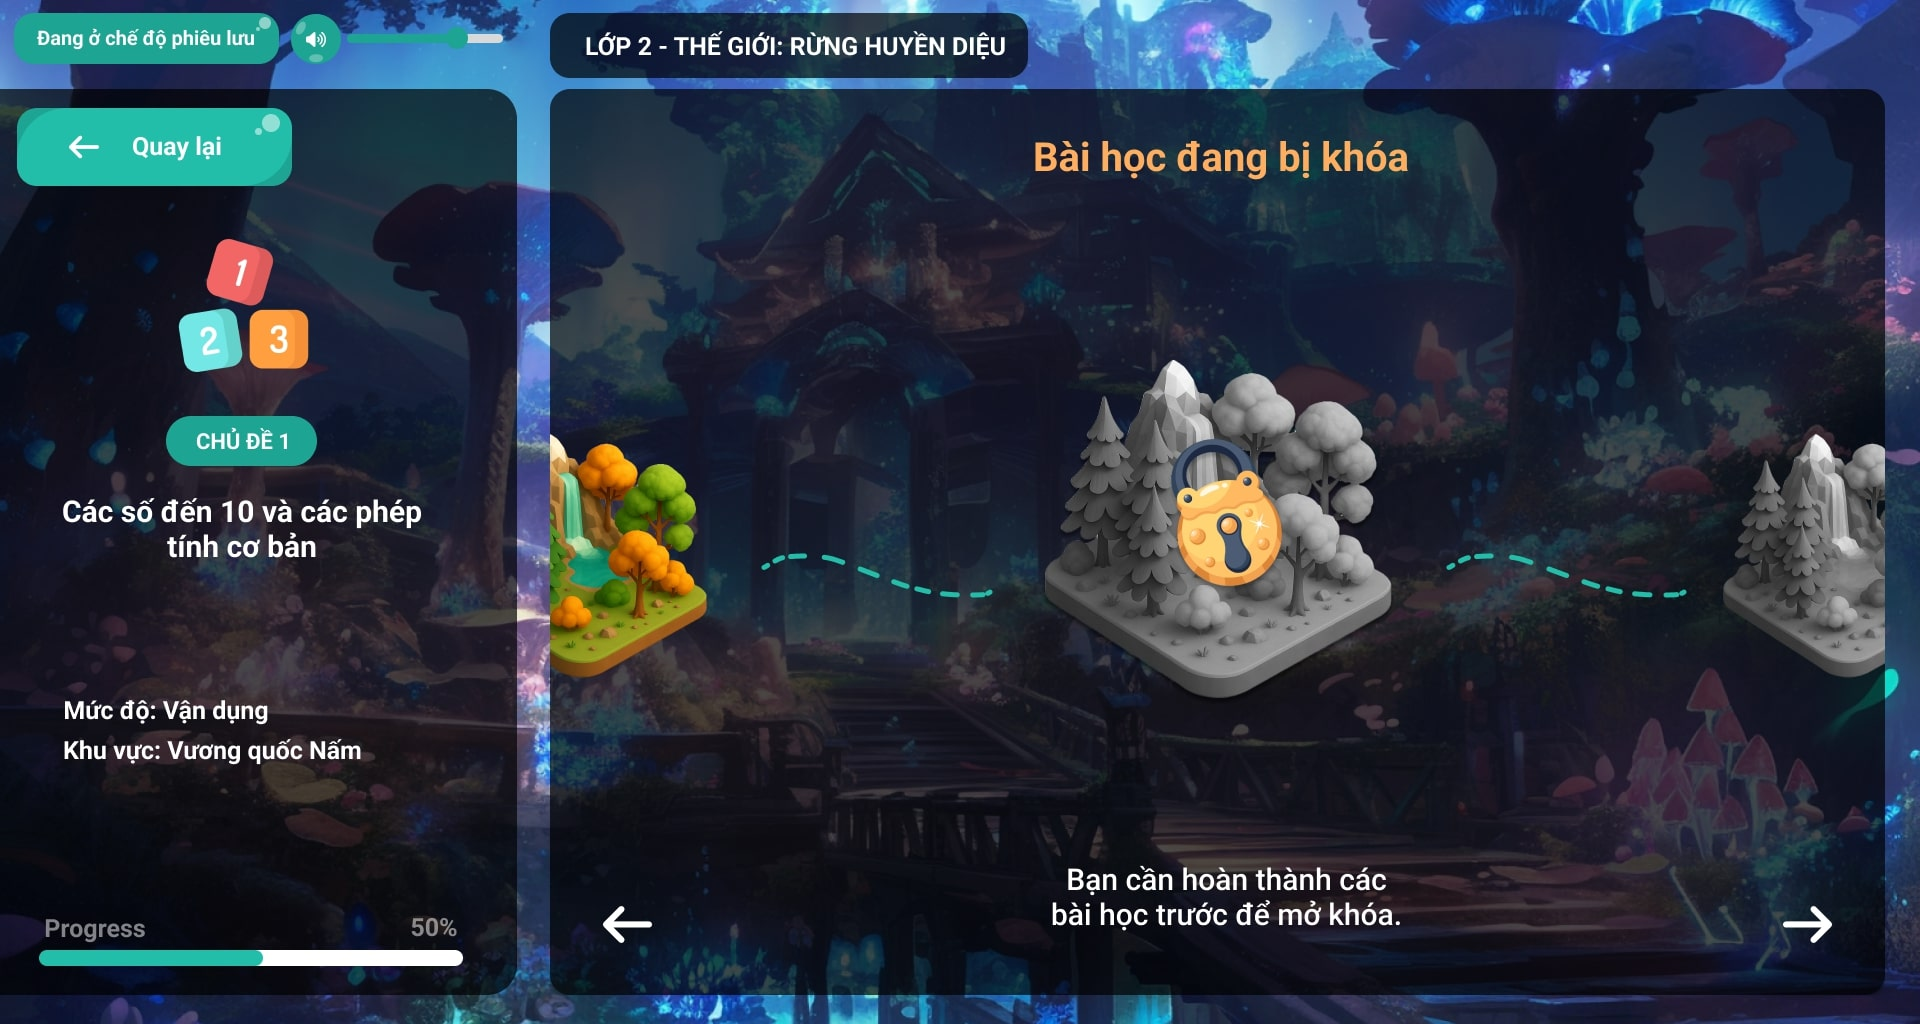
\includegraphics[width=\textwidth]{Image/UI/Milestones/Paths-G2-Locked.jpg}
			\vspace{0.2cm}
			\caption{Lớp 2 - Milestone bị khóa}
			\label{fig:l2}
		\end{minipage}
	\end{figure}
	
	\vspace{0.4cm}
	
	% --- Trang Chủ đề của Lớp 3 ---
	\noindent Thế giới của Lớp 3 được thiết kế với bối cảnh biển cả. Các hình từ \ref{fig:e3} đến \ref{fig:h3} là thiết kế cho trang chủ đề của lớp 3 ứng với các mức độ khó khác nhau của bài học. Giao diện khóa của các bài học (milestone) được thiết kế như \textit{Hình \ref{fig:l3}}.
	\begin{figure}[H]
		\centering
		\begin{minipage}{0.45\textwidth}
			\centering
			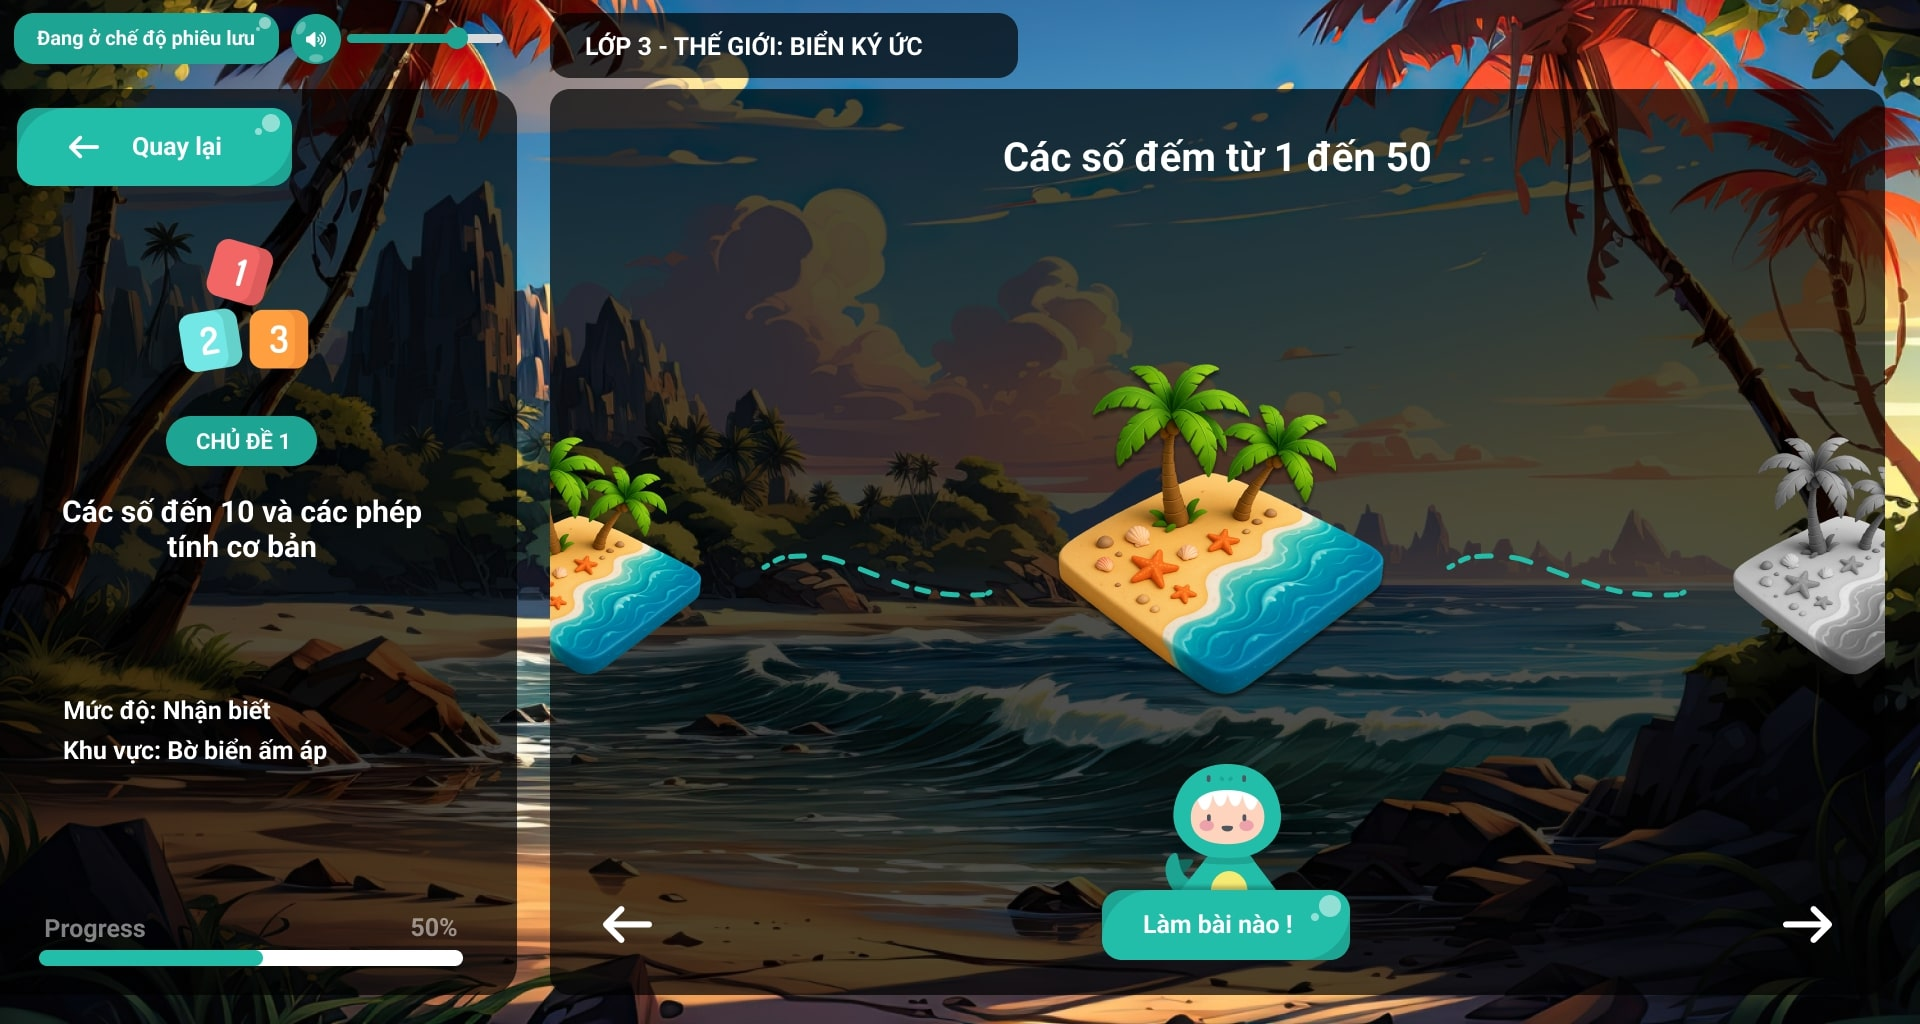
\includegraphics[width=\textwidth]{Image/UI/Milestones/Paths-G3-NB.jpg}
			\vspace{0.2cm}
			\caption{Lớp 3 - Nhận biết}
			\label{fig:e3}
		\end{minipage}
		\hspace{0.1cm}
		\begin{minipage}{0.45\textwidth}
			\centering
			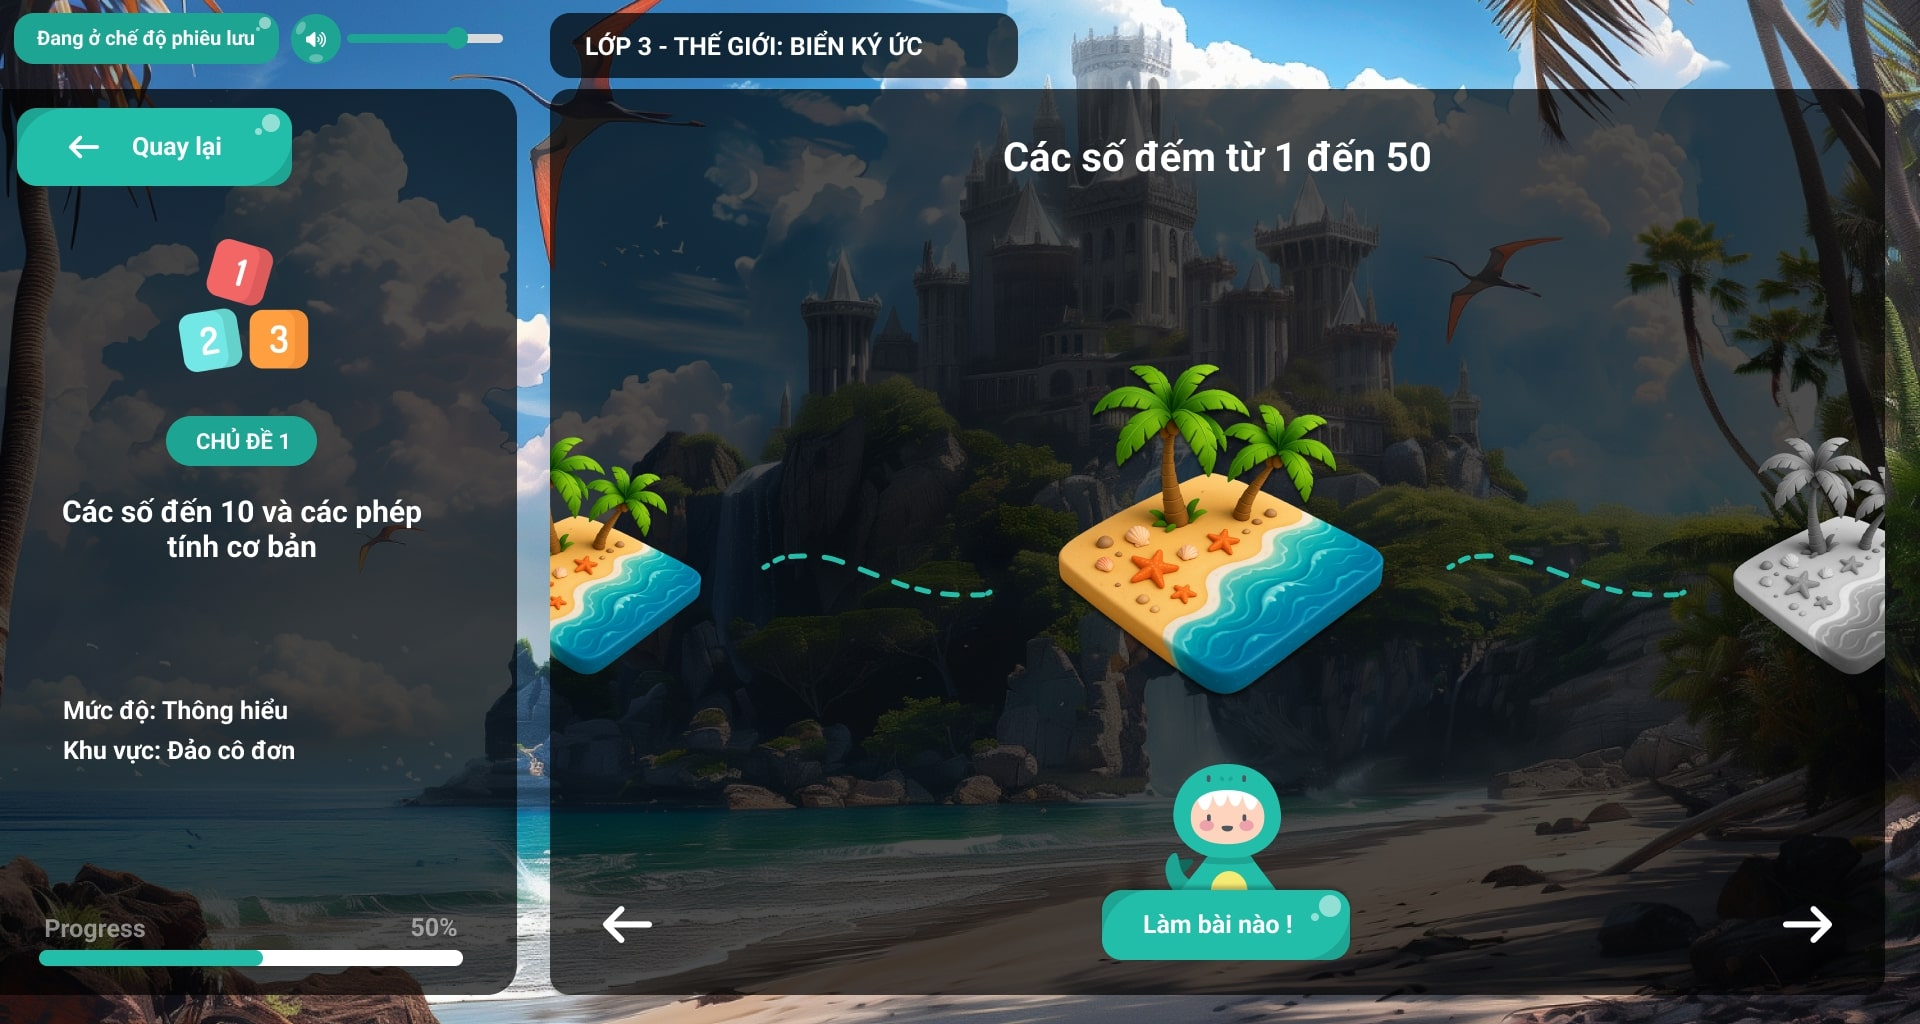
\includegraphics[width=\textwidth]{Image/UI/Milestones/Paths-G3-TH.jpg}
			\vspace{0.2cm}
			\caption{Lớp 3 - Thông hiểu}
		\end{minipage}
		
		\vspace{0.4cm}
		
		\begin{minipage}{0.45\textwidth}
			\centering
			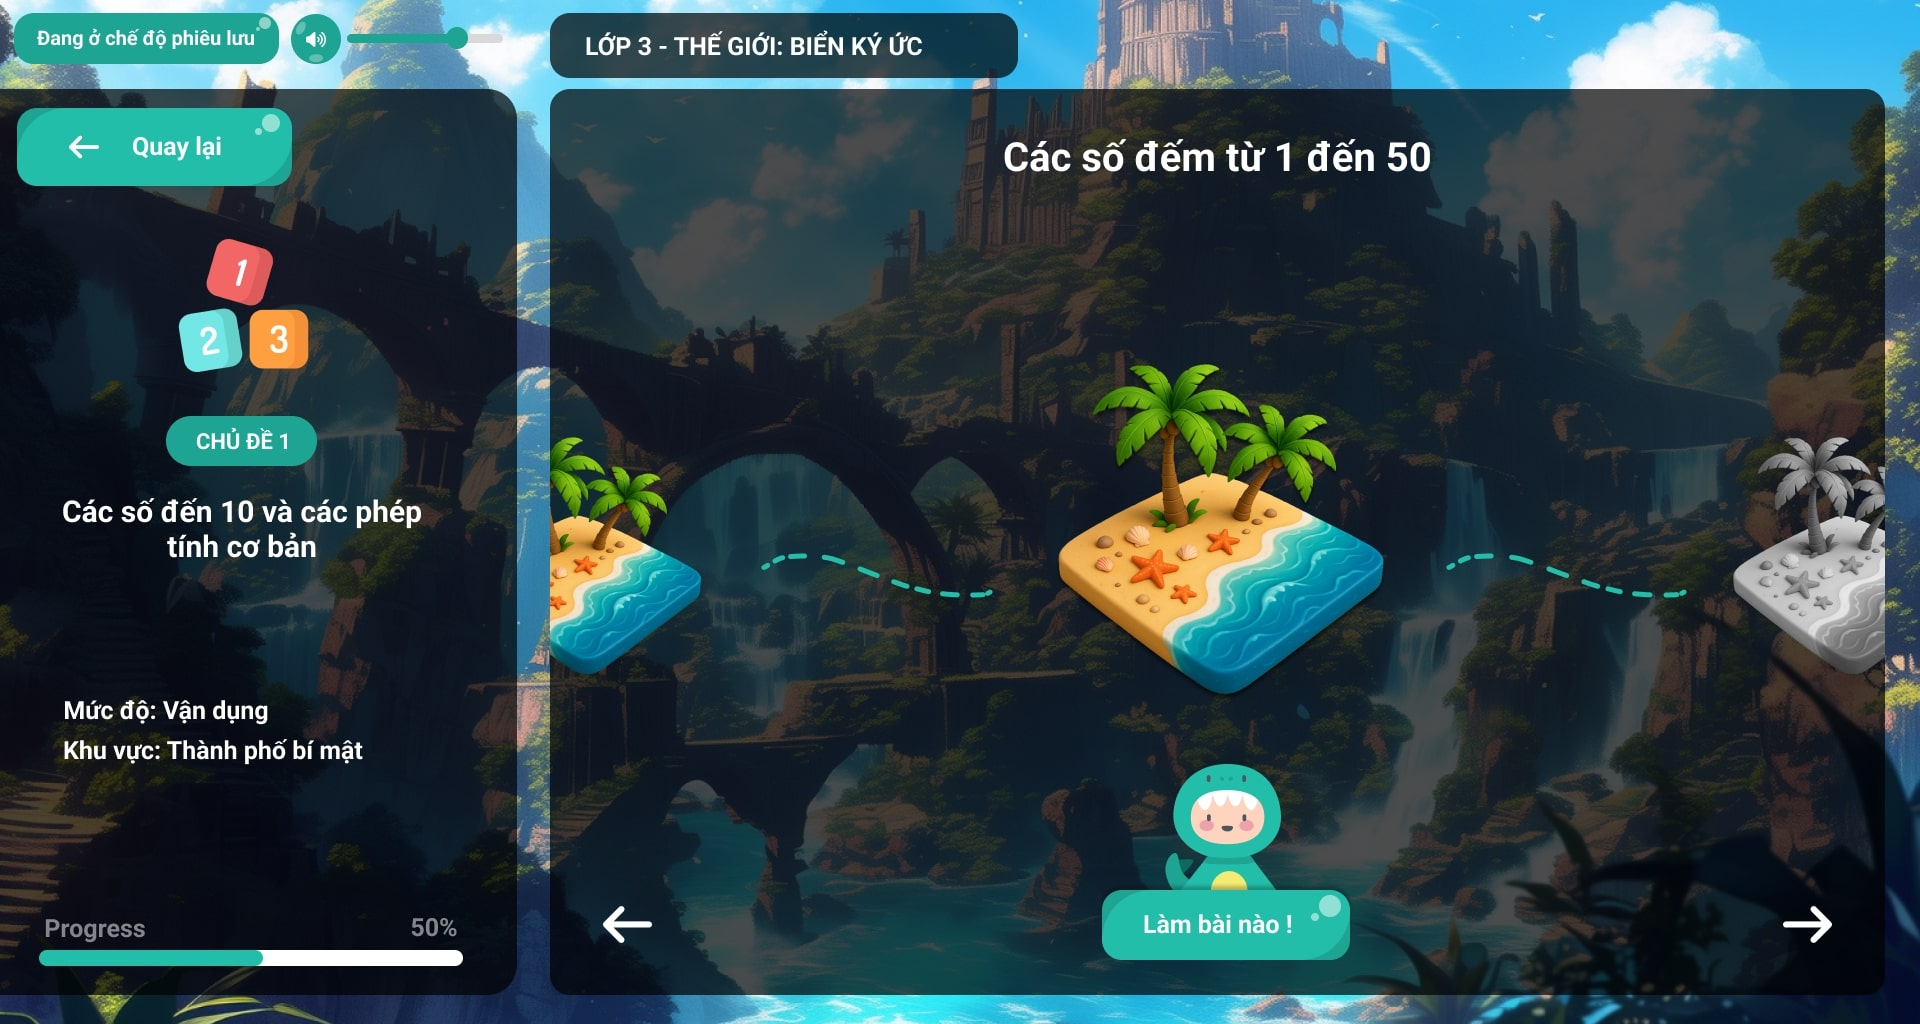
\includegraphics[width=\textwidth]{Image/UI/Milestones/Paths-G3-VD.jpg}
			\vspace{0.2cm}
			\caption{Lớp 3 - Vận dụng}
			\label{fig:h3}
		\end{minipage}
		\hspace{0.1cm}
		\begin{minipage}{0.45\textwidth}
			\centering
			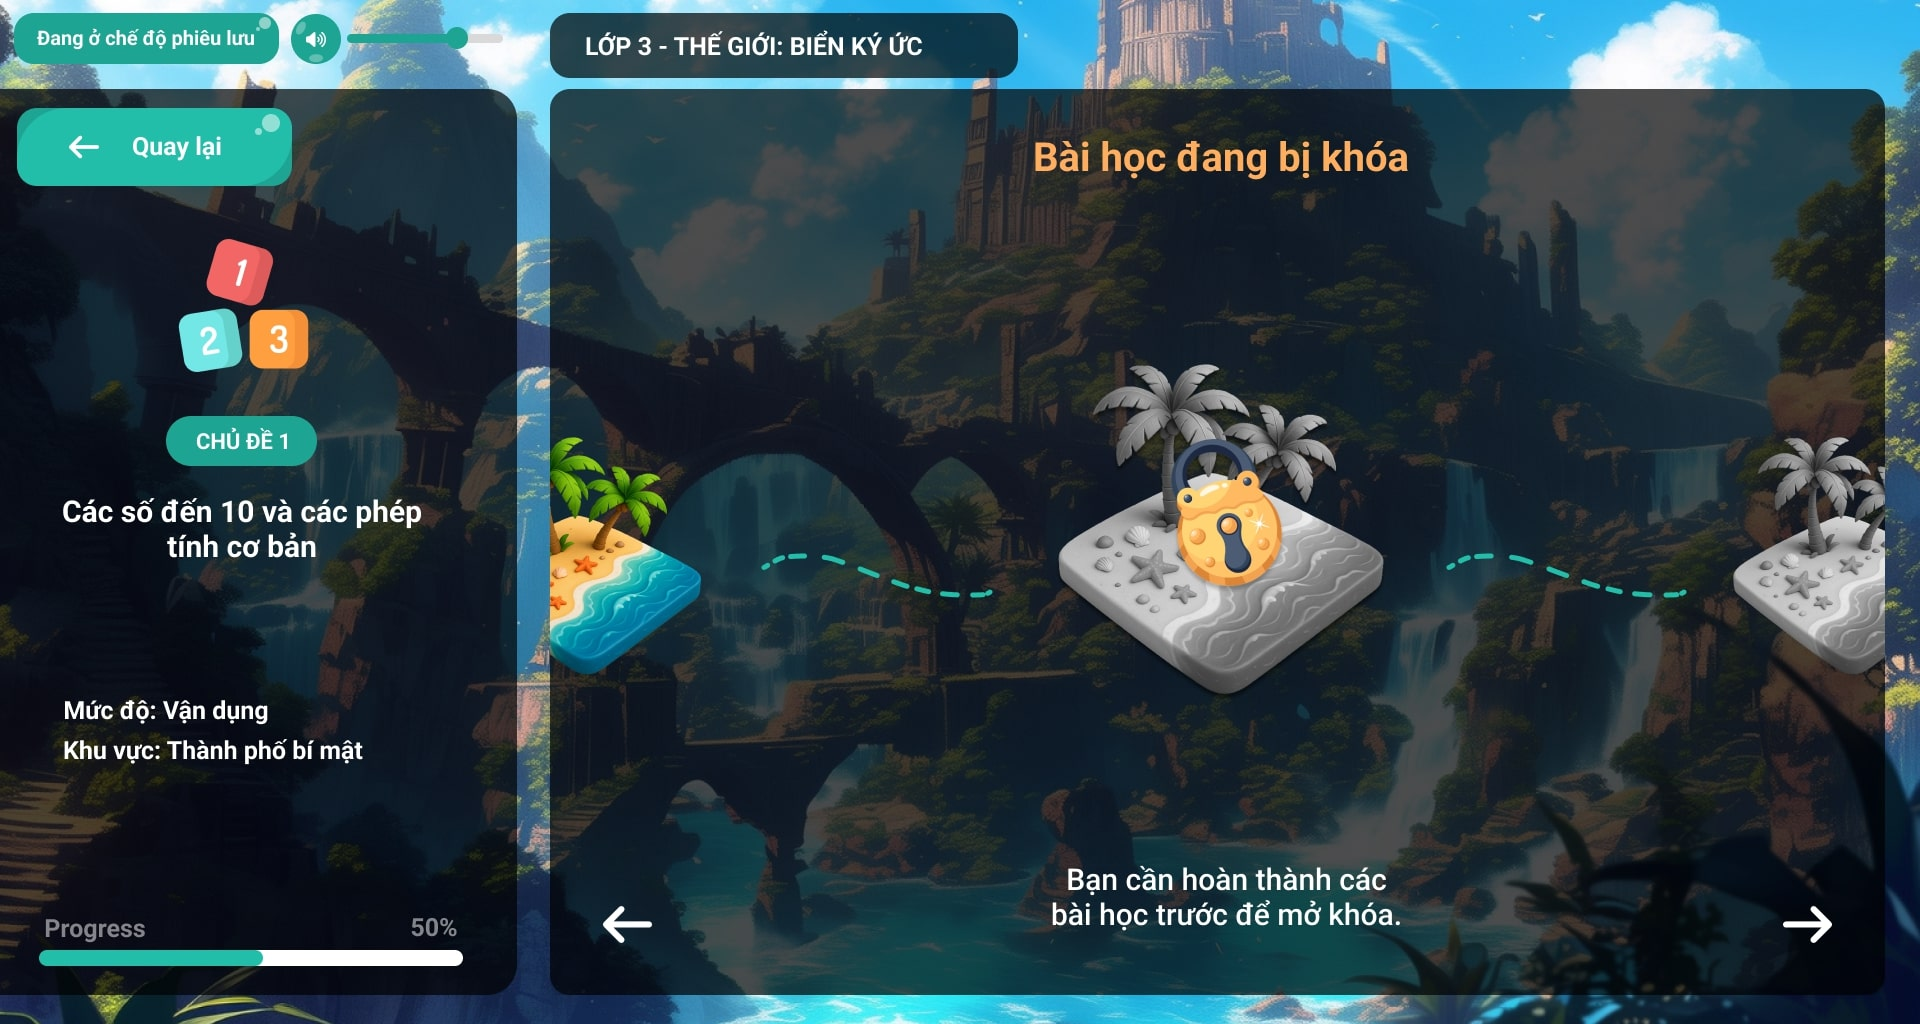
\includegraphics[width=\textwidth]{Image/UI/Milestones/Paths-G3-Locked.jpg}
			\vspace{0.2cm}
			\caption{Lớp 3 - Milestone bị khóa}
			\label{fig:l3}
		\end{minipage}
	\end{figure}
	
	\vspace{0.4cm}
	
	% --- Trang Chủ đề của Lớp 4 ---
	\noindent Thế giới của Lớp 4 được thiết kế với bối cảnh sa mạc. Các hình từ \ref{fig:e4} đến \ref{fig:h4} là thiết kế cho trang chủ đề của lớp 4 ứng với các mức độ khó khác nhau của bài học. Giao diện khóa của các bài học (milestone) được thiết kế như \textit{Hình \ref{fig:l4}}.
	\begin{figure}[H]
		\centering
		\begin{minipage}{0.45\textwidth}
			\centering
			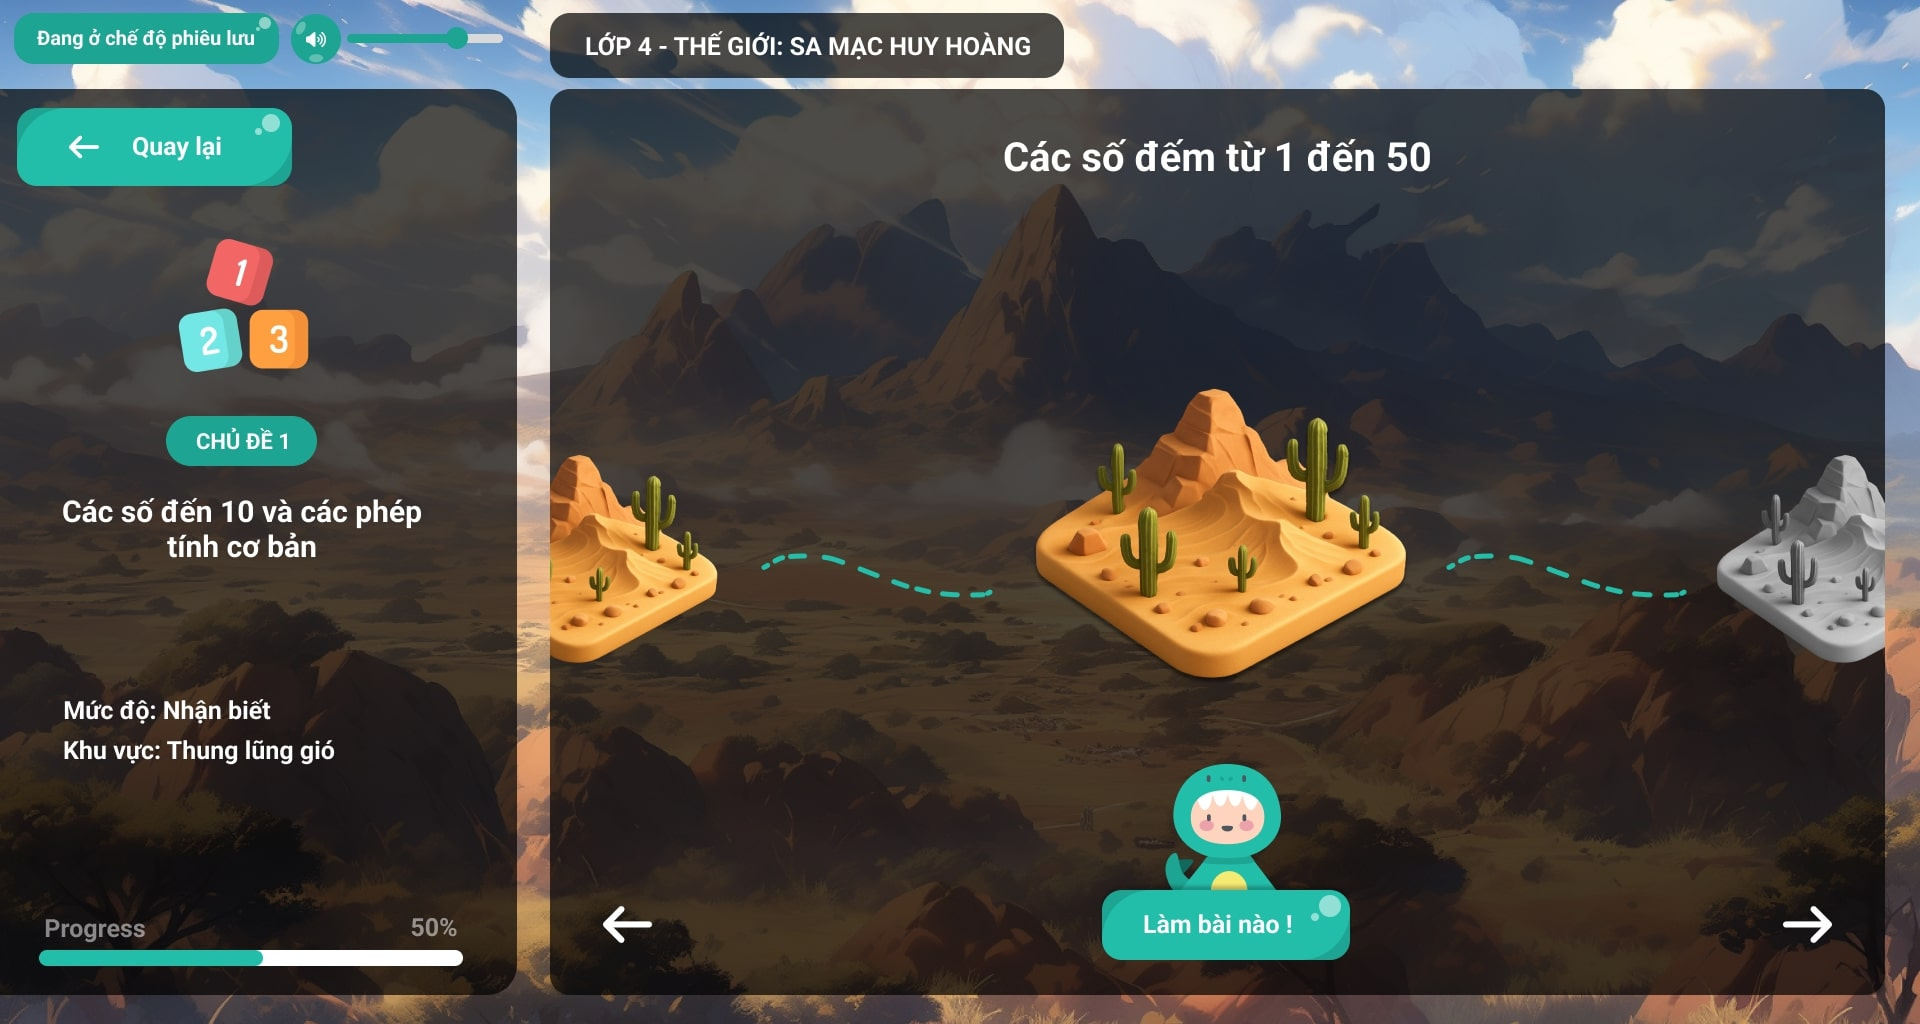
\includegraphics[width=\textwidth]{Image/UI/Milestones/Paths-G4-NB.jpg}
			\vspace{0.2cm}
			\caption{Lớp 4 - Nhận biết}
			\label{fig:e4}
		\end{minipage}
		\hspace{0.1cm}
		\begin{minipage}{0.45\textwidth}
			\centering
			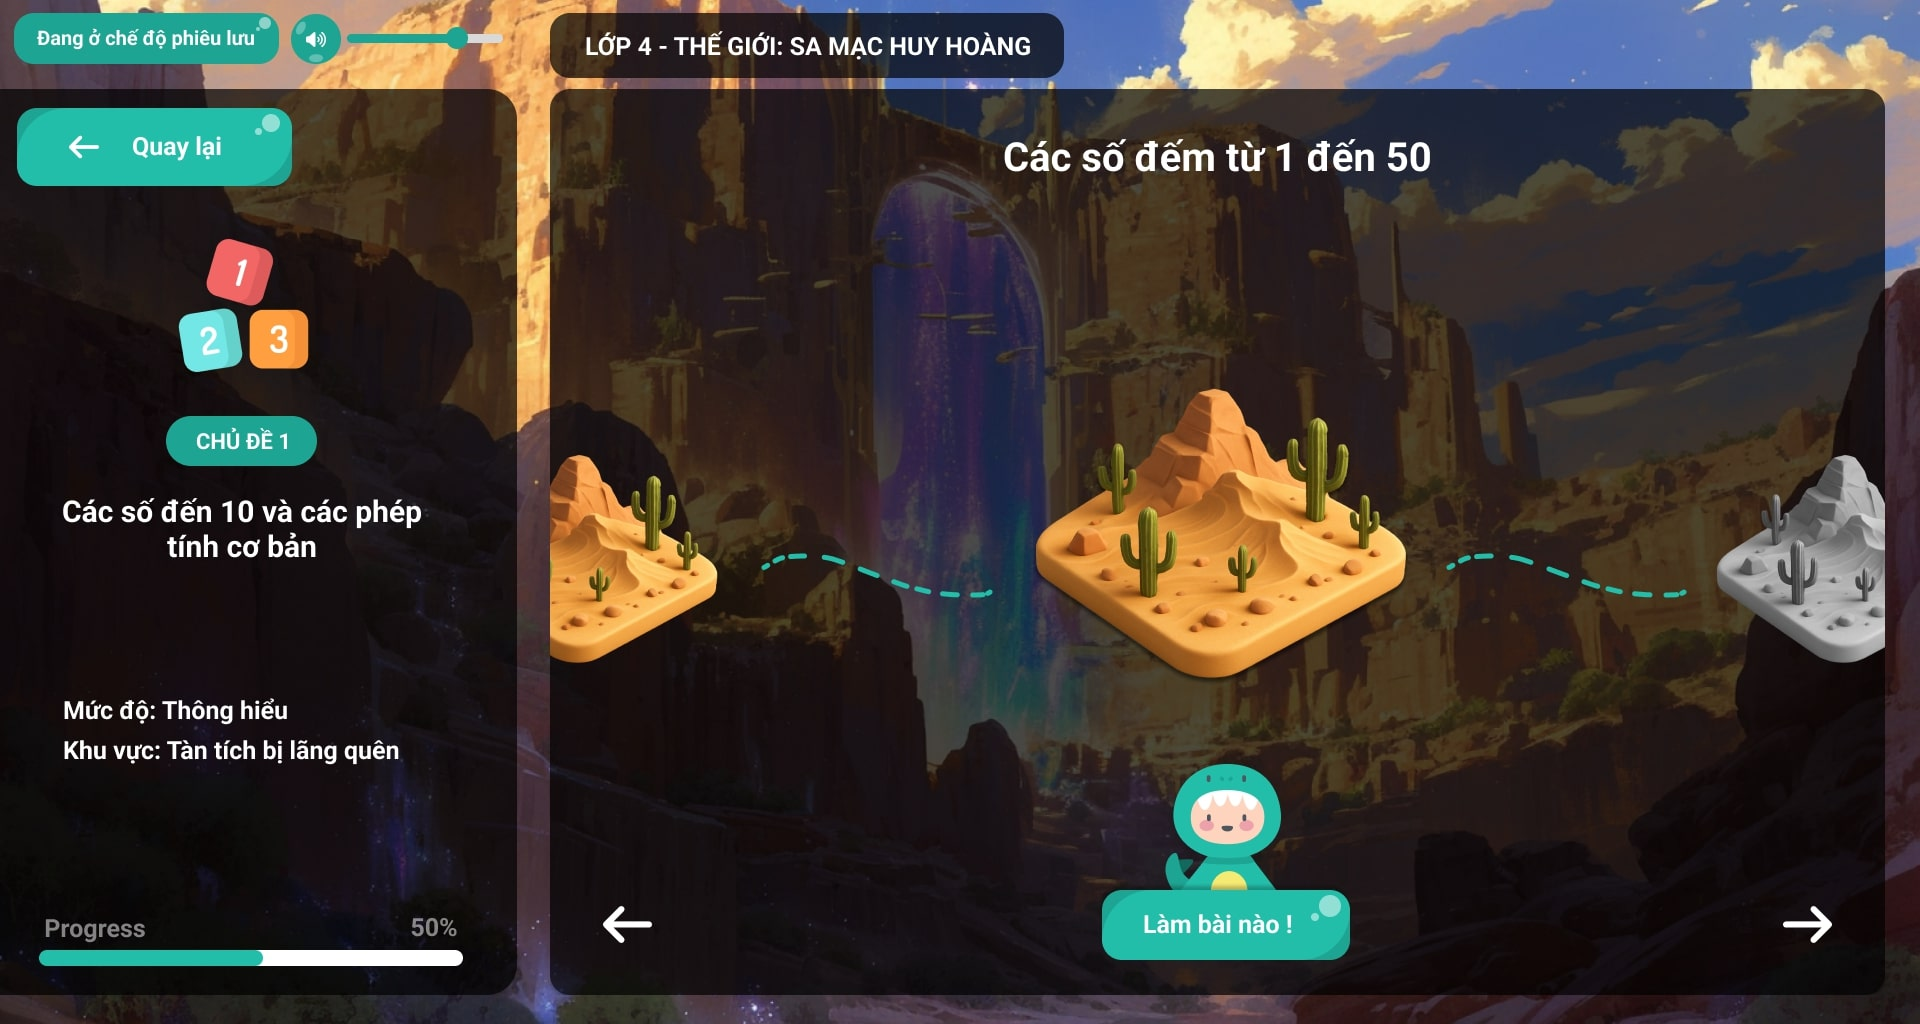
\includegraphics[width=\textwidth]{Image/UI/Milestones/Paths-G4-TH.jpg}
			\vspace{0.2cm}
			\caption{Lớp 4 - Thông hiểu}
		\end{minipage}
		
		\vspace{0.4cm}
		
		\begin{minipage}{0.45\textwidth}
			\centering
			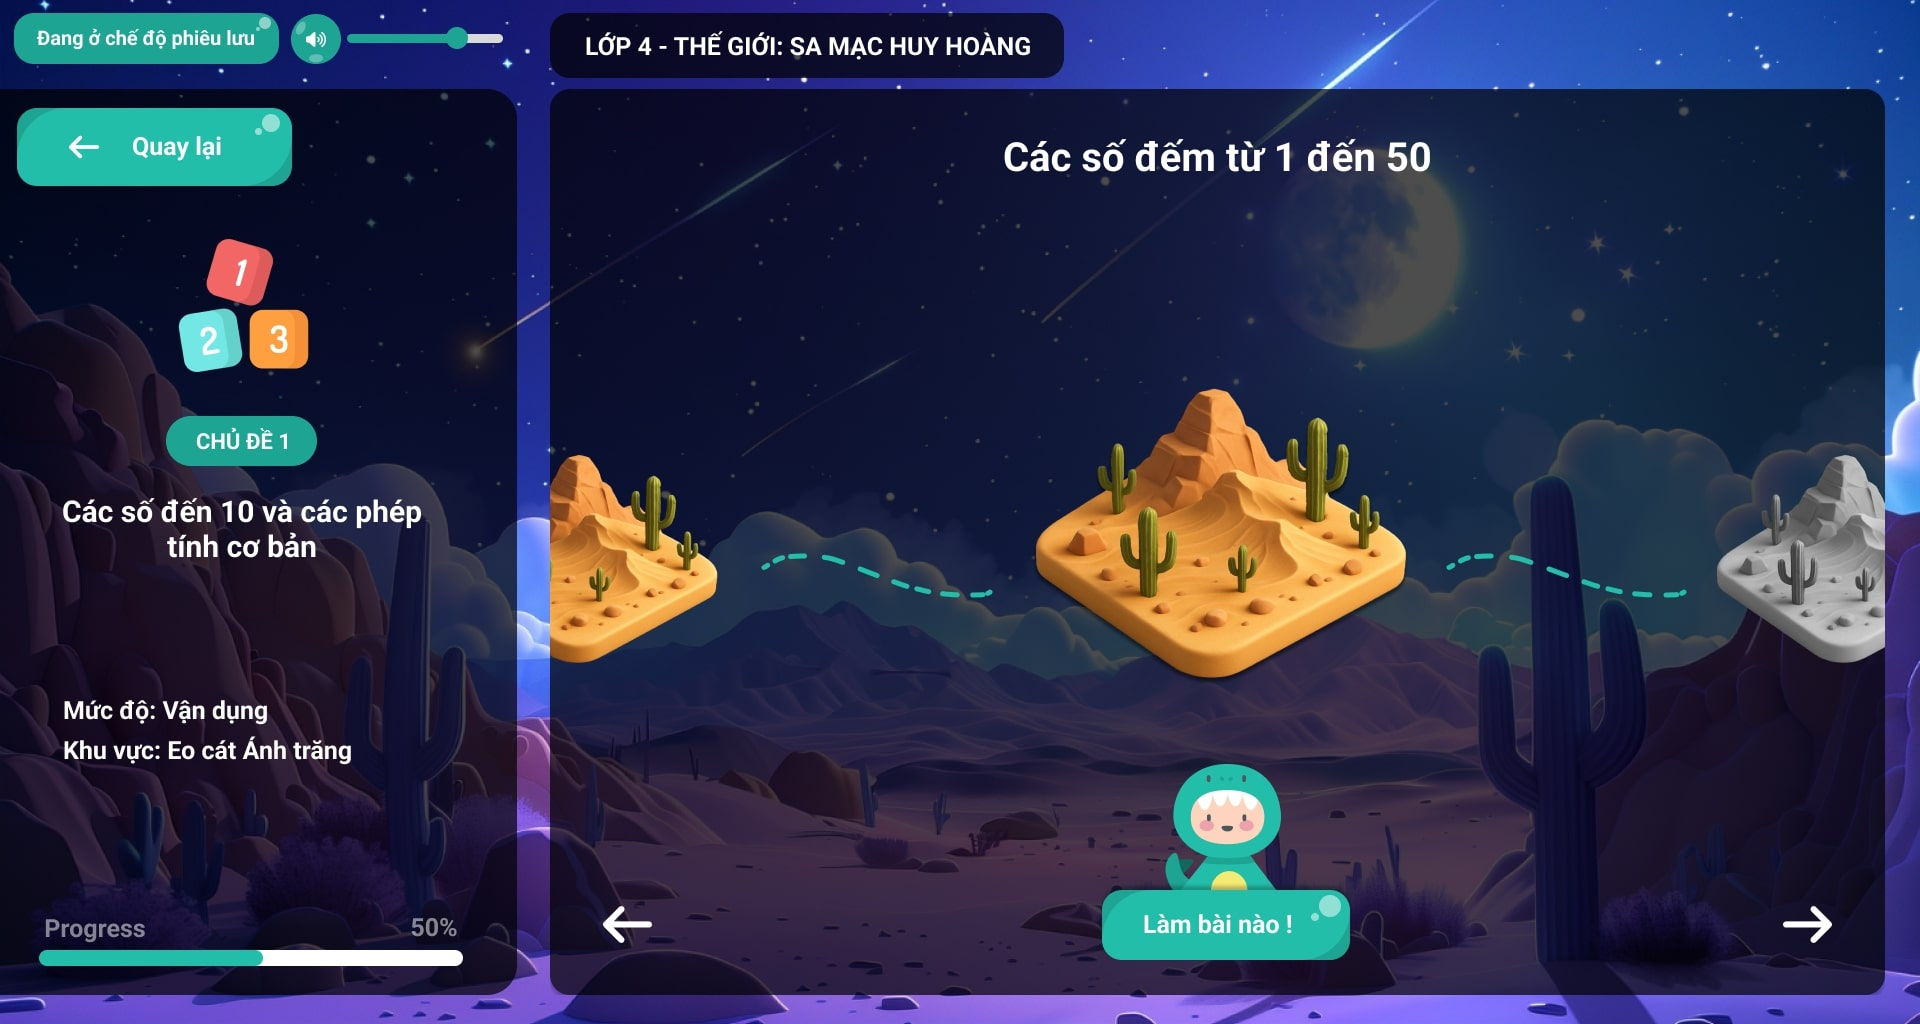
\includegraphics[width=\textwidth]{Image/UI/Milestones/Paths-G4-VD.jpg}
			\vspace{0.2cm}
			\caption{Lớp 4 - Vận dụng}
			\label{fig:h4}
		\end{minipage}
		\hspace{0.1cm}
		\begin{minipage}{0.45\textwidth}
			\centering
			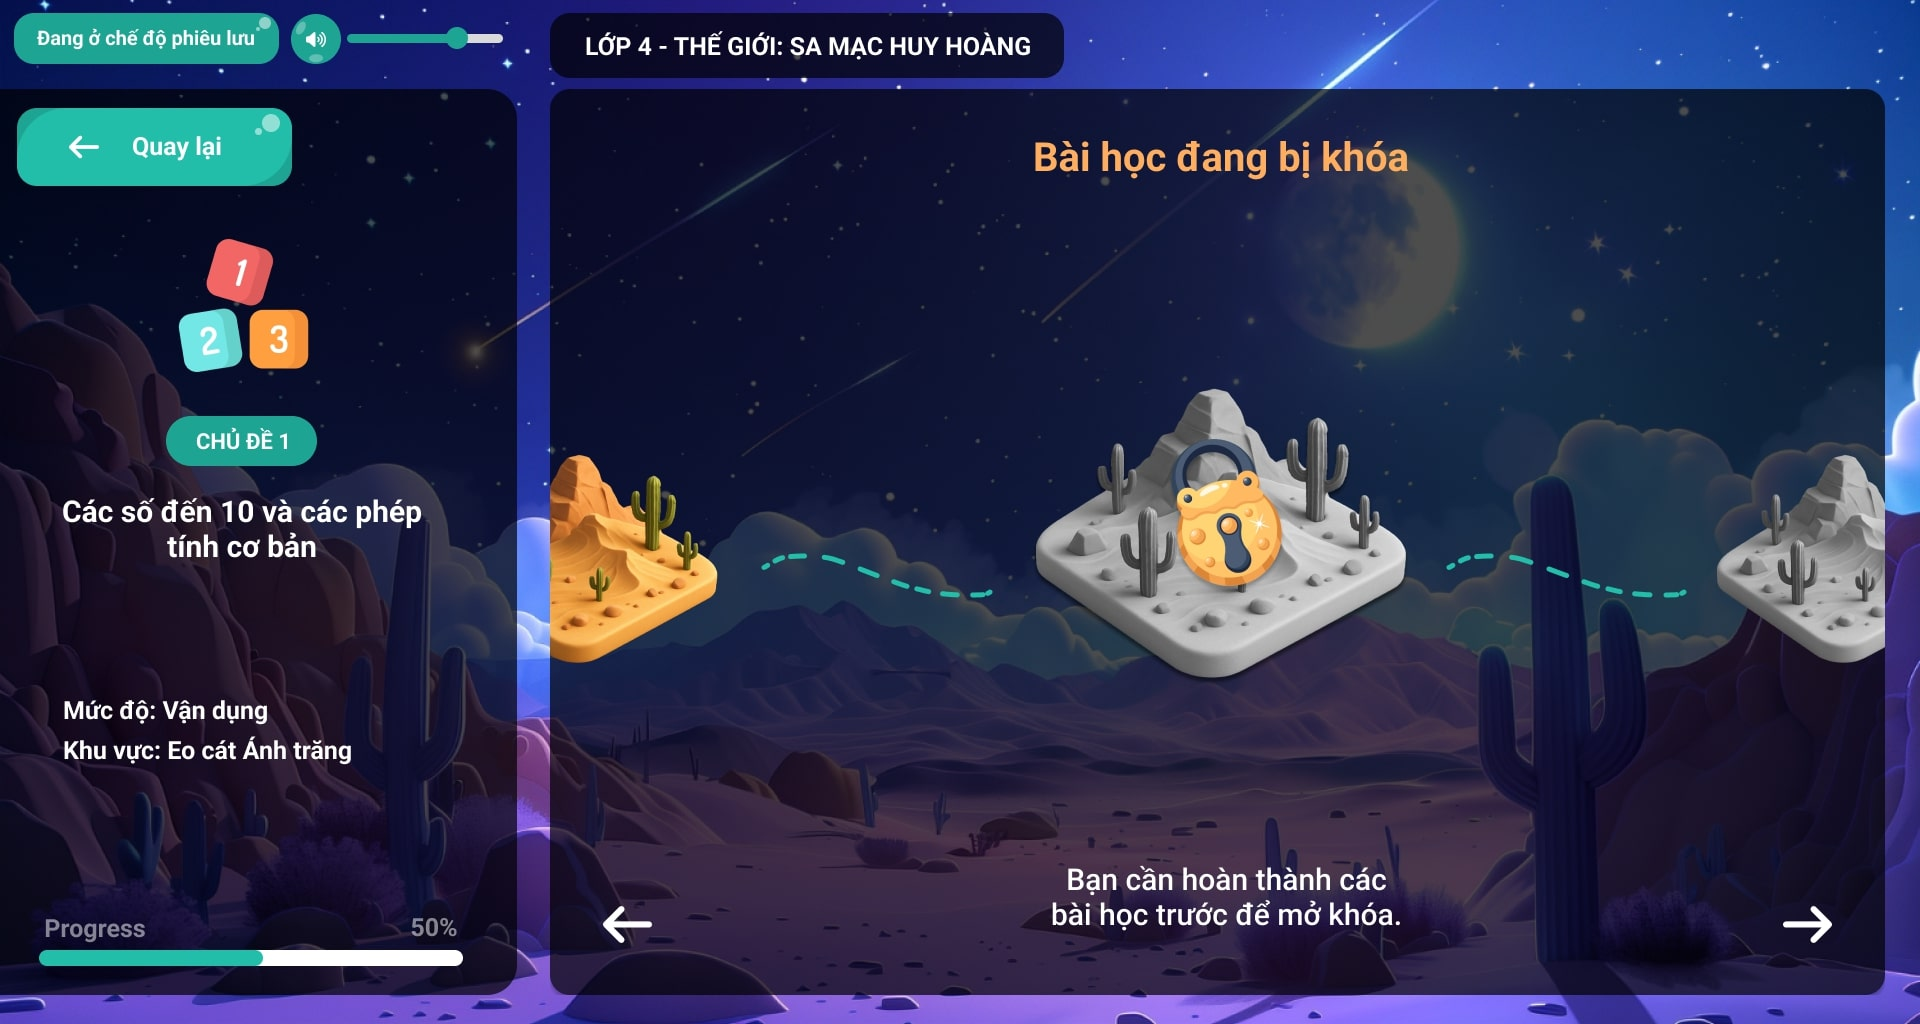
\includegraphics[width=\textwidth]{Image/UI/Milestones/Paths-G4-Locked.jpg}
			\vspace{0.2cm}
			\caption{Lớp 4 - Milestone bị khóa}
			\label{fig:l4}
		\end{minipage}
	\end{figure}
	
	\vspace{0.4cm}
	
	% --- Trang Chủ đề của Lớp 5 ---
	\noindent Thế giới của Lớp 5 được thiết kế với bối cảnh núi lửa. Các hình từ \ref{fig:e5} đến \ref{fig:h5} là thiết kế cho trang chủ đề của lớp 5 ứng với các mức độ khó khác nhau của bài học. Giao diện khóa của các bài học (milestone) được thiết kế như \textit{Hình \ref{fig:l5}}.
	\begin{figure}[H]
		\centering
		\begin{minipage}{0.45\textwidth}
			\centering
			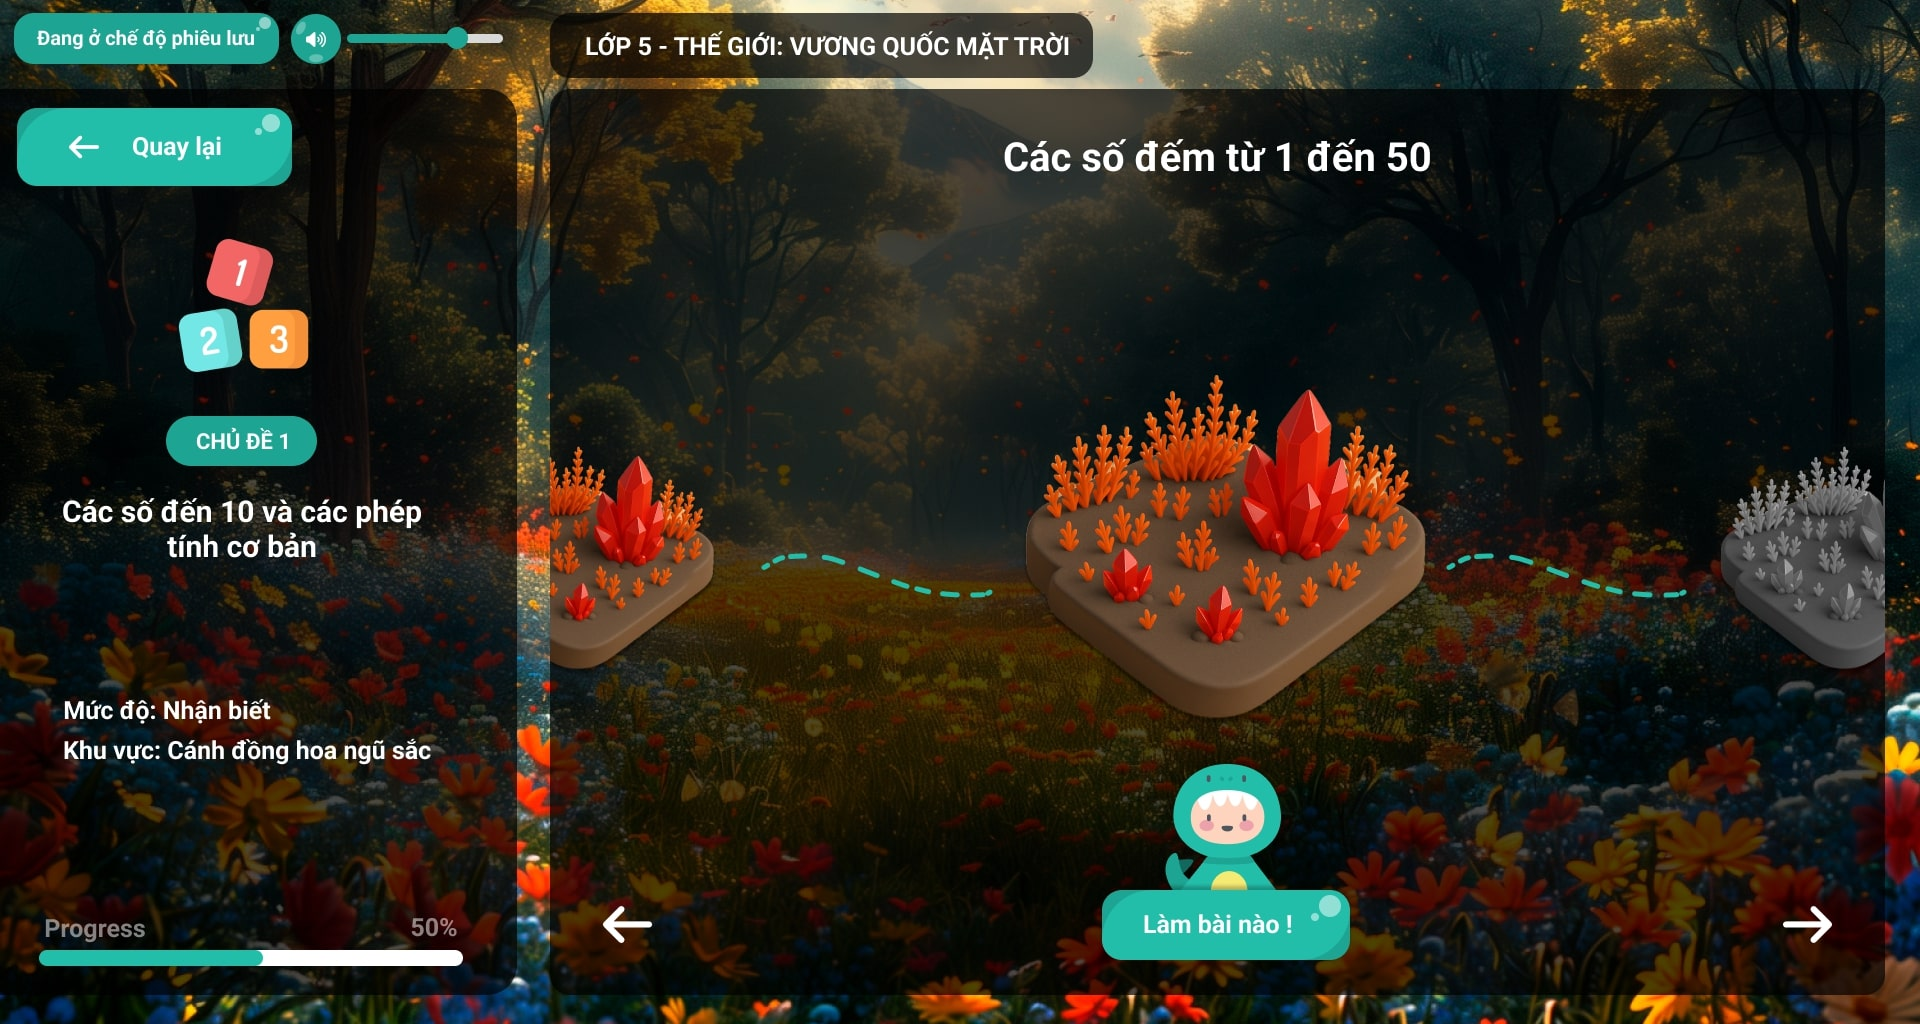
\includegraphics[width=\textwidth]{Image/UI/Milestones/Paths-G5-NB.jpg}
			\vspace{0.2cm}
			\caption{Lớp 5 - Nhận biết}
			\label{fig:e5}
		\end{minipage}
		\hspace{0.1cm}
		\begin{minipage}{0.45\textwidth}
			\centering
			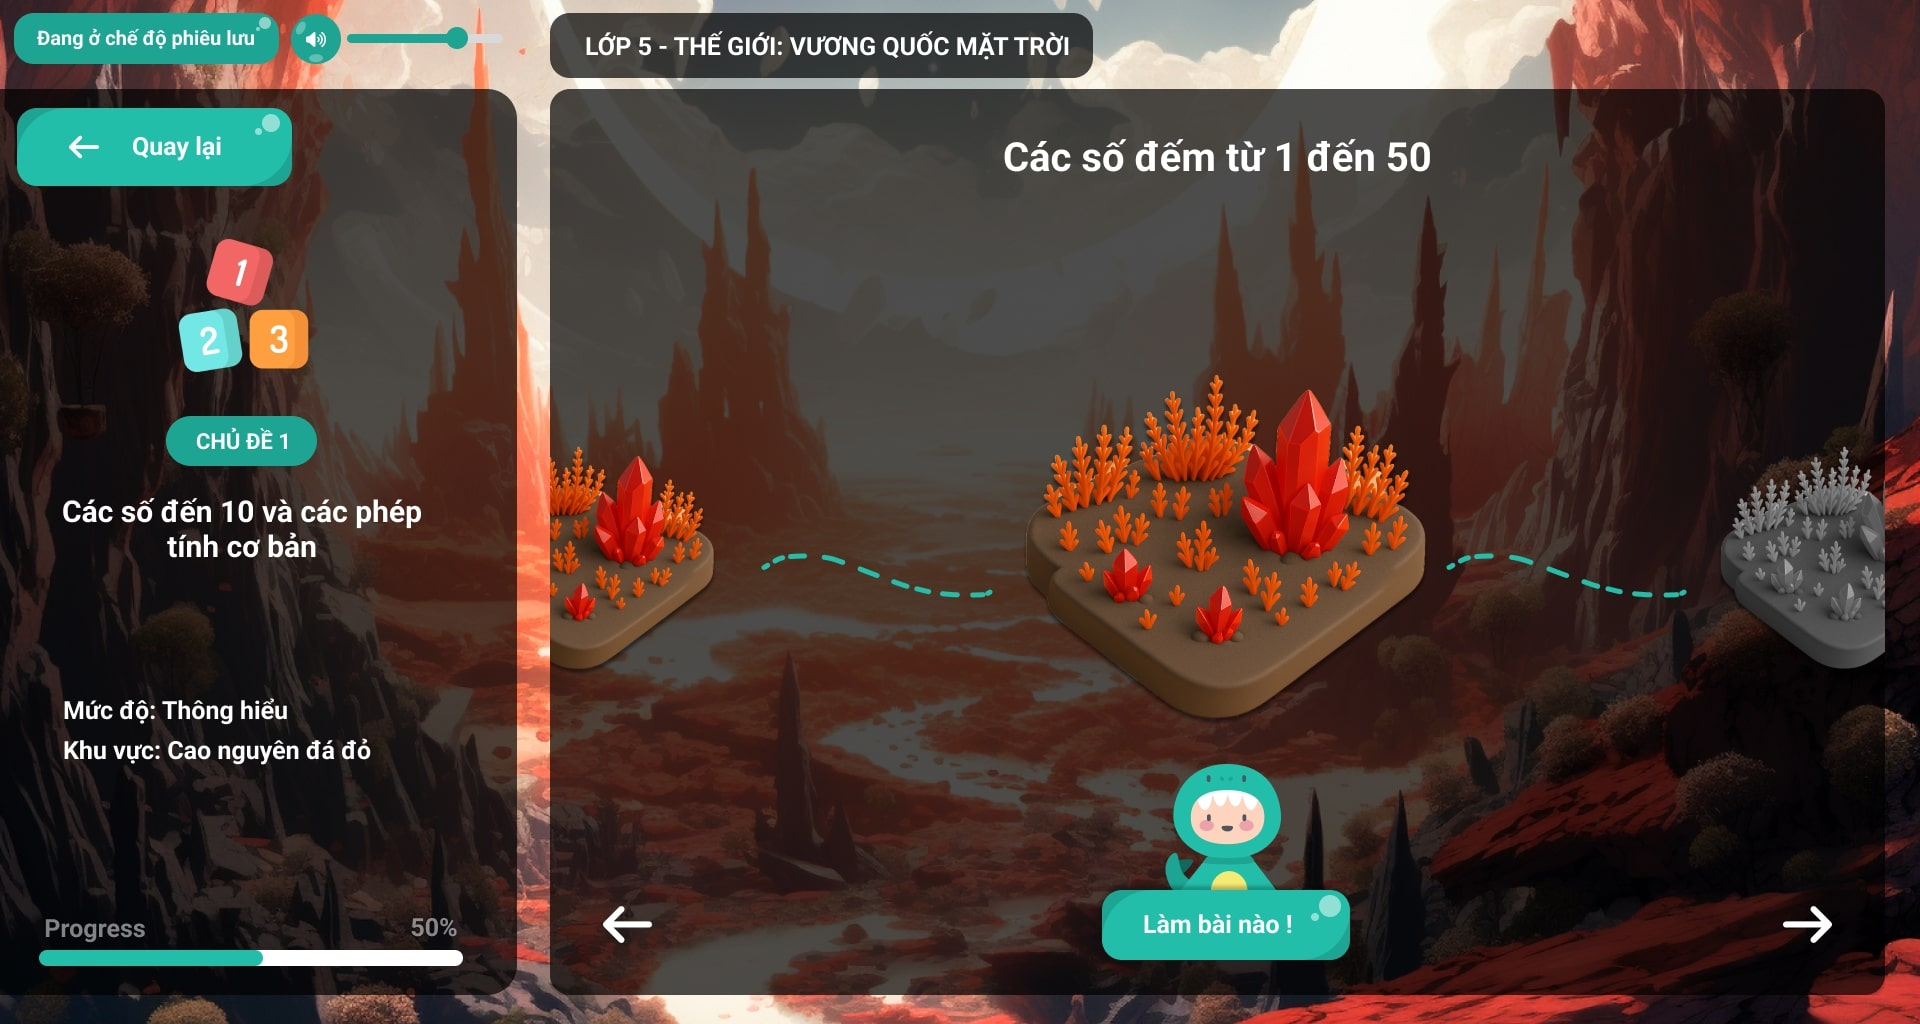
\includegraphics[width=\textwidth]{Image/UI/Milestones/Paths-G5-TH.jpg}
			\vspace{0.2cm}
			\caption{Lớp 5 - Thông hiểu}
		\end{minipage}
		
		\vspace{0.4cm}
		
		\begin{minipage}{0.45\textwidth}
			\centering
			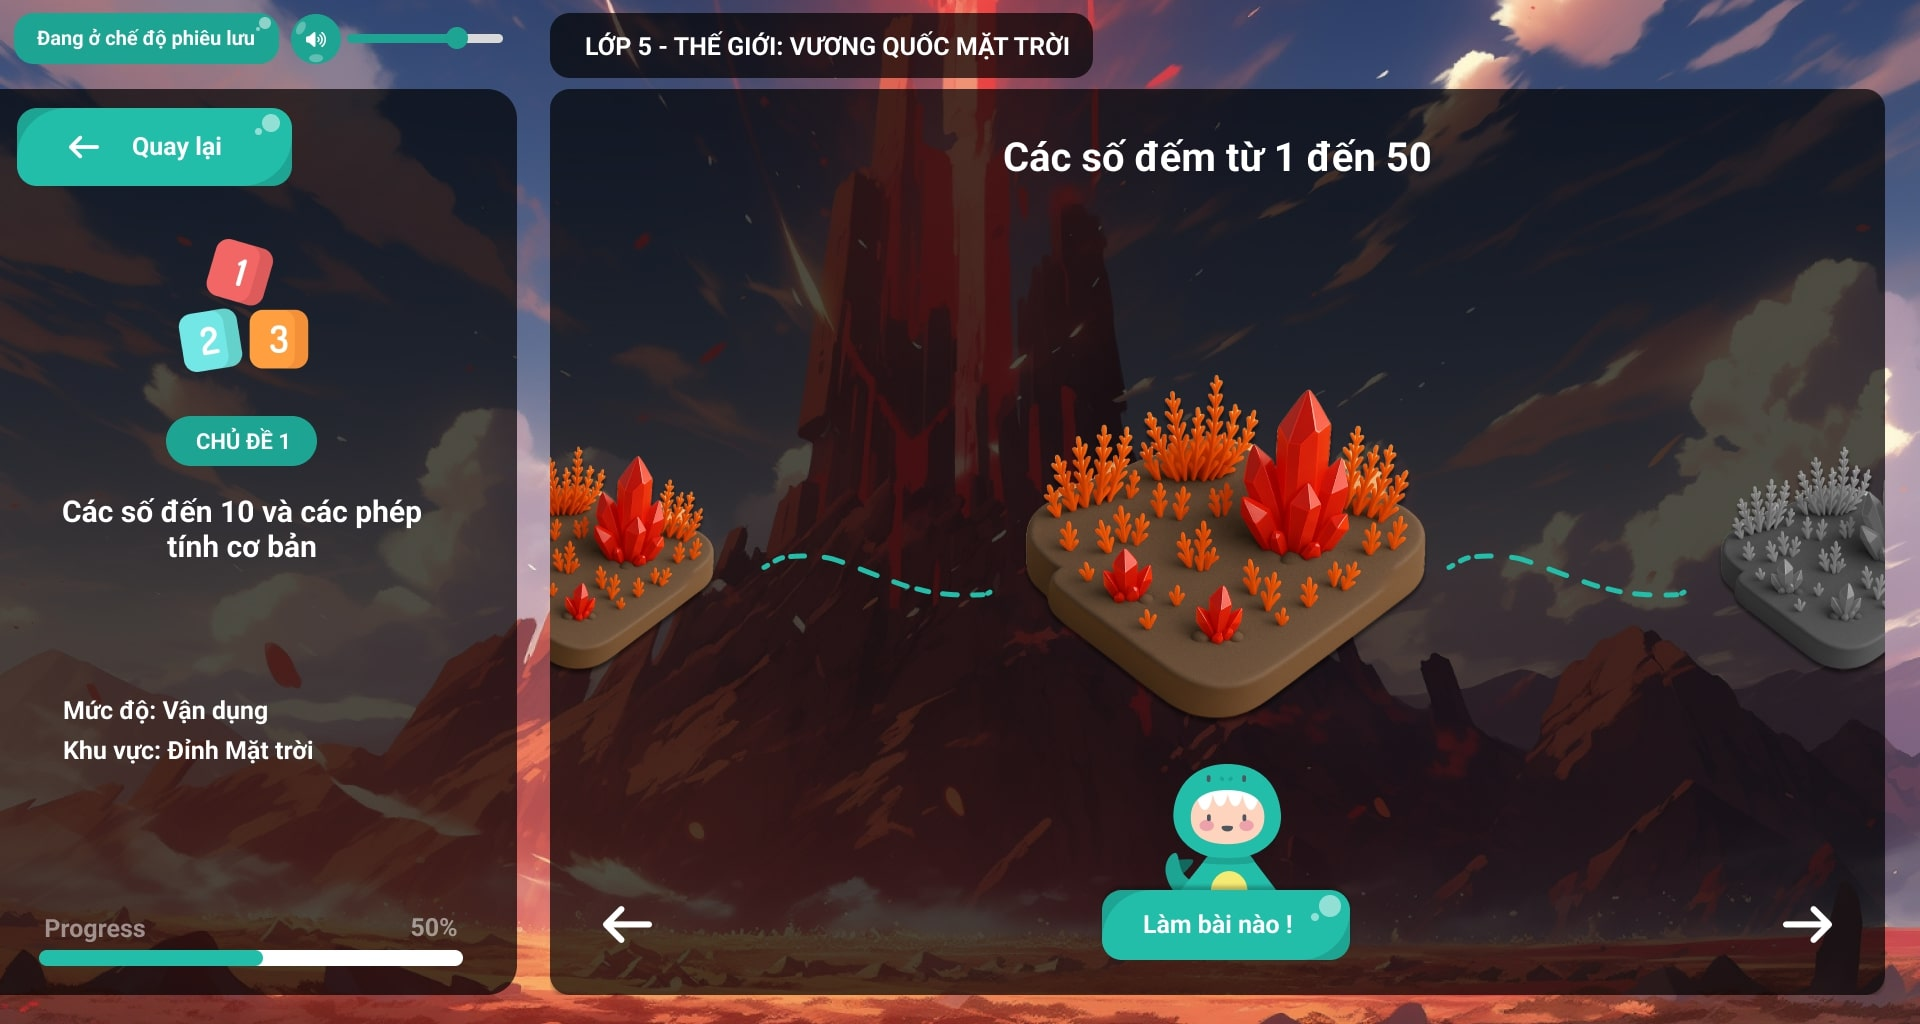
\includegraphics[width=\textwidth]{Image/UI/Milestones/Paths-G5-VD.jpg}
			\vspace{0.2cm}
			\caption{Lớp 5 - Vận dụng}
			\label{fig:h5}
		\end{minipage}
		\hspace{0.1cm}
		\begin{minipage}{0.45\textwidth}
			\centering
			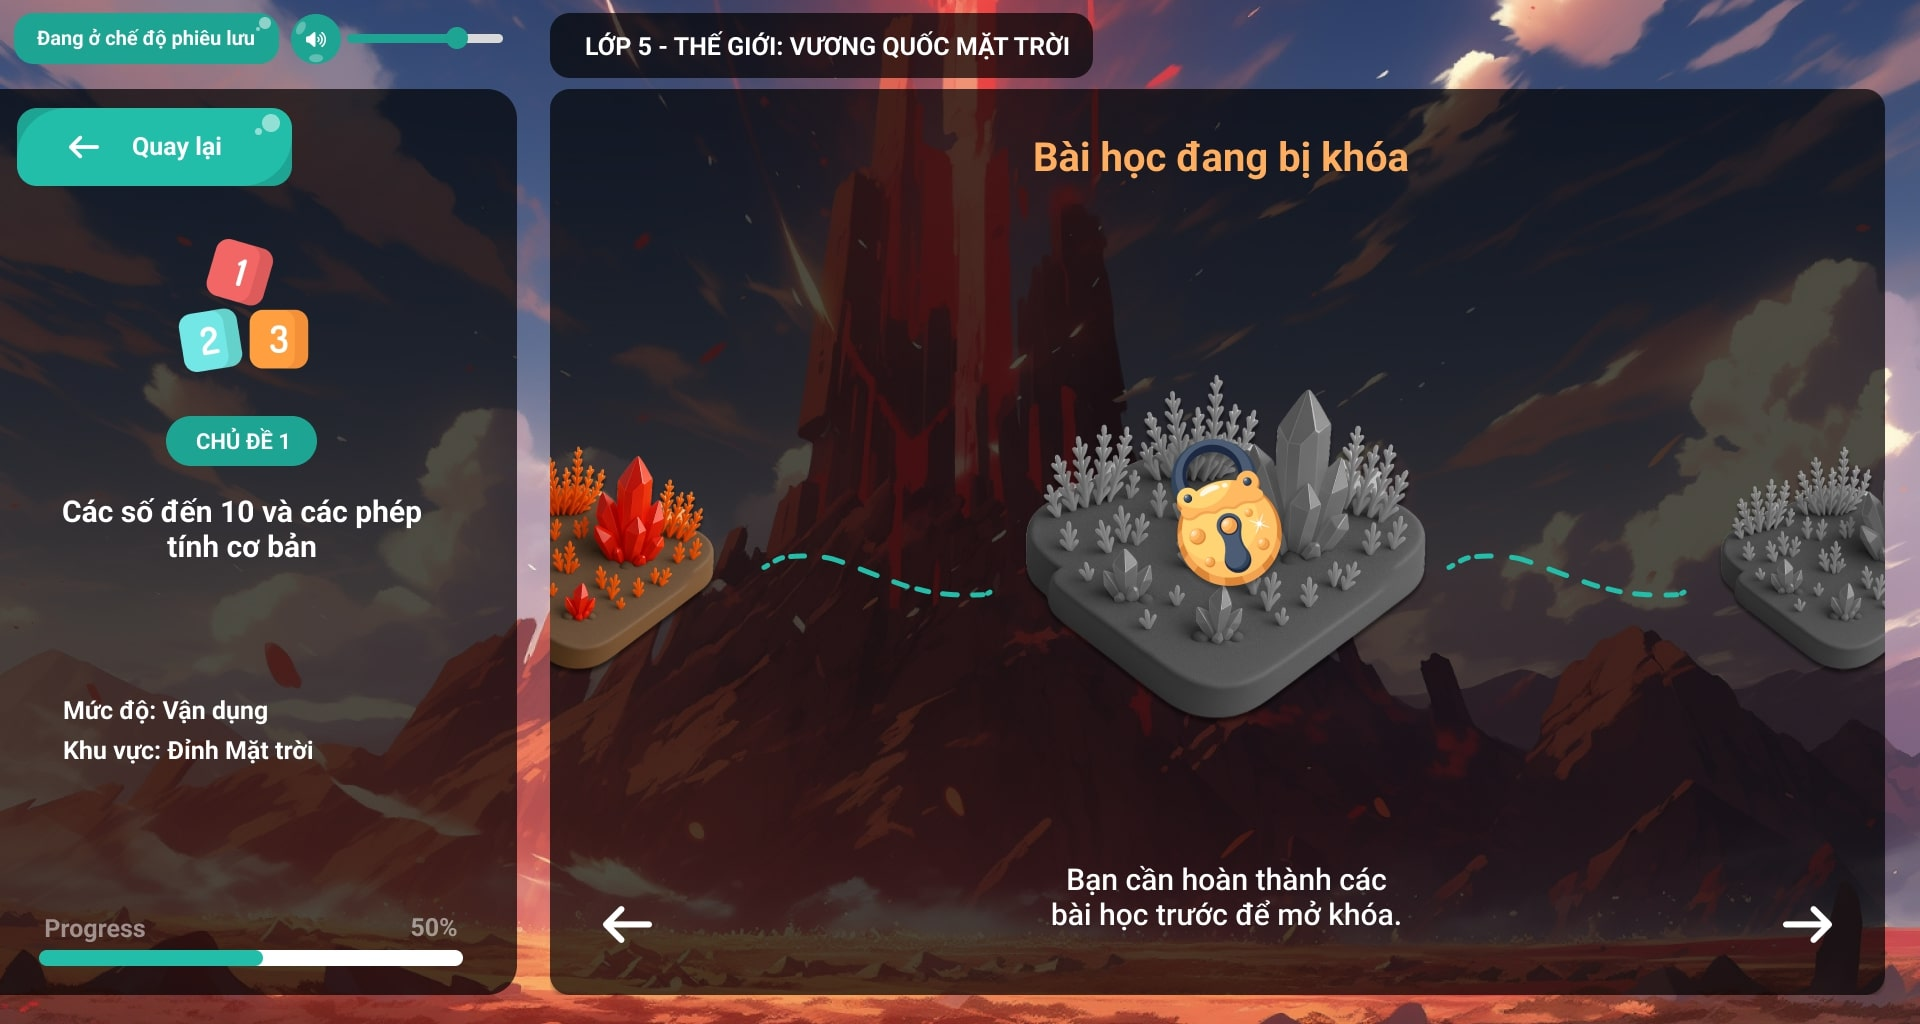
\includegraphics[width=\textwidth]{Image/UI/Milestones/Paths-G5-Locked.jpg}
			\vspace{0.2cm}
			\caption{Lớp 5 - Milestone bị khóa}
			\label{fig:l5}
		\end{minipage}
	\end{figure}

\subsubsection{Trang Bài tập}
\label{subsubsec:exercise}
\textbf{Trang Bài tập} chỉ có thể được truy cập bằng cách bấm vào nút \textit{Làm bài} ở \textbf{Trang Chủ đề} được mô tả ở mục \ref{subsubsec:topic}. Tại trang này người dùng có thể làm các dạng bài tập tương tác như kéo thả, trắc nghiệm, đúng/sai, điền khuyết, lắp ghép (xem chi tiết ở mục \ref{subsec:interact}). Phần tên bài học và danh sách các câu hỏi được hiển thị trên sidebar nằm bên trái giao diện. Người dùng có thể chuyển câu hỏi bằng cách nhấn vào các nút được đánh số thứ tự tương ứng. Người dùng có thể nộp bài bằng cách bấm vào nút \textit{Nộp bài} ở dưới cùng của sidebar. Với mỗi câu làm đúng, người dùng sẽ nhận được một lượng thạch anh nhất định. Giao diện làm bài tập hỗ trợ nhiều dạng tương tác khác nhau (xem chi tiết tại mục \ref{subsec:interact}).

\newline
Sau khi tương tác với bài tập, người dùng có thể bấm \textit{Kiểm tra đáp án} để kiểm tra câu trả lời của mình. Nếu trả lời đúng, giao diện sẽ giống như \textit{Hình \ref{fig:correct}}; nếu sai, giao diện sẽ giống như \textit{Hình \ref{fig:wrong}}.
\begin{figure}[H]
	\centering
	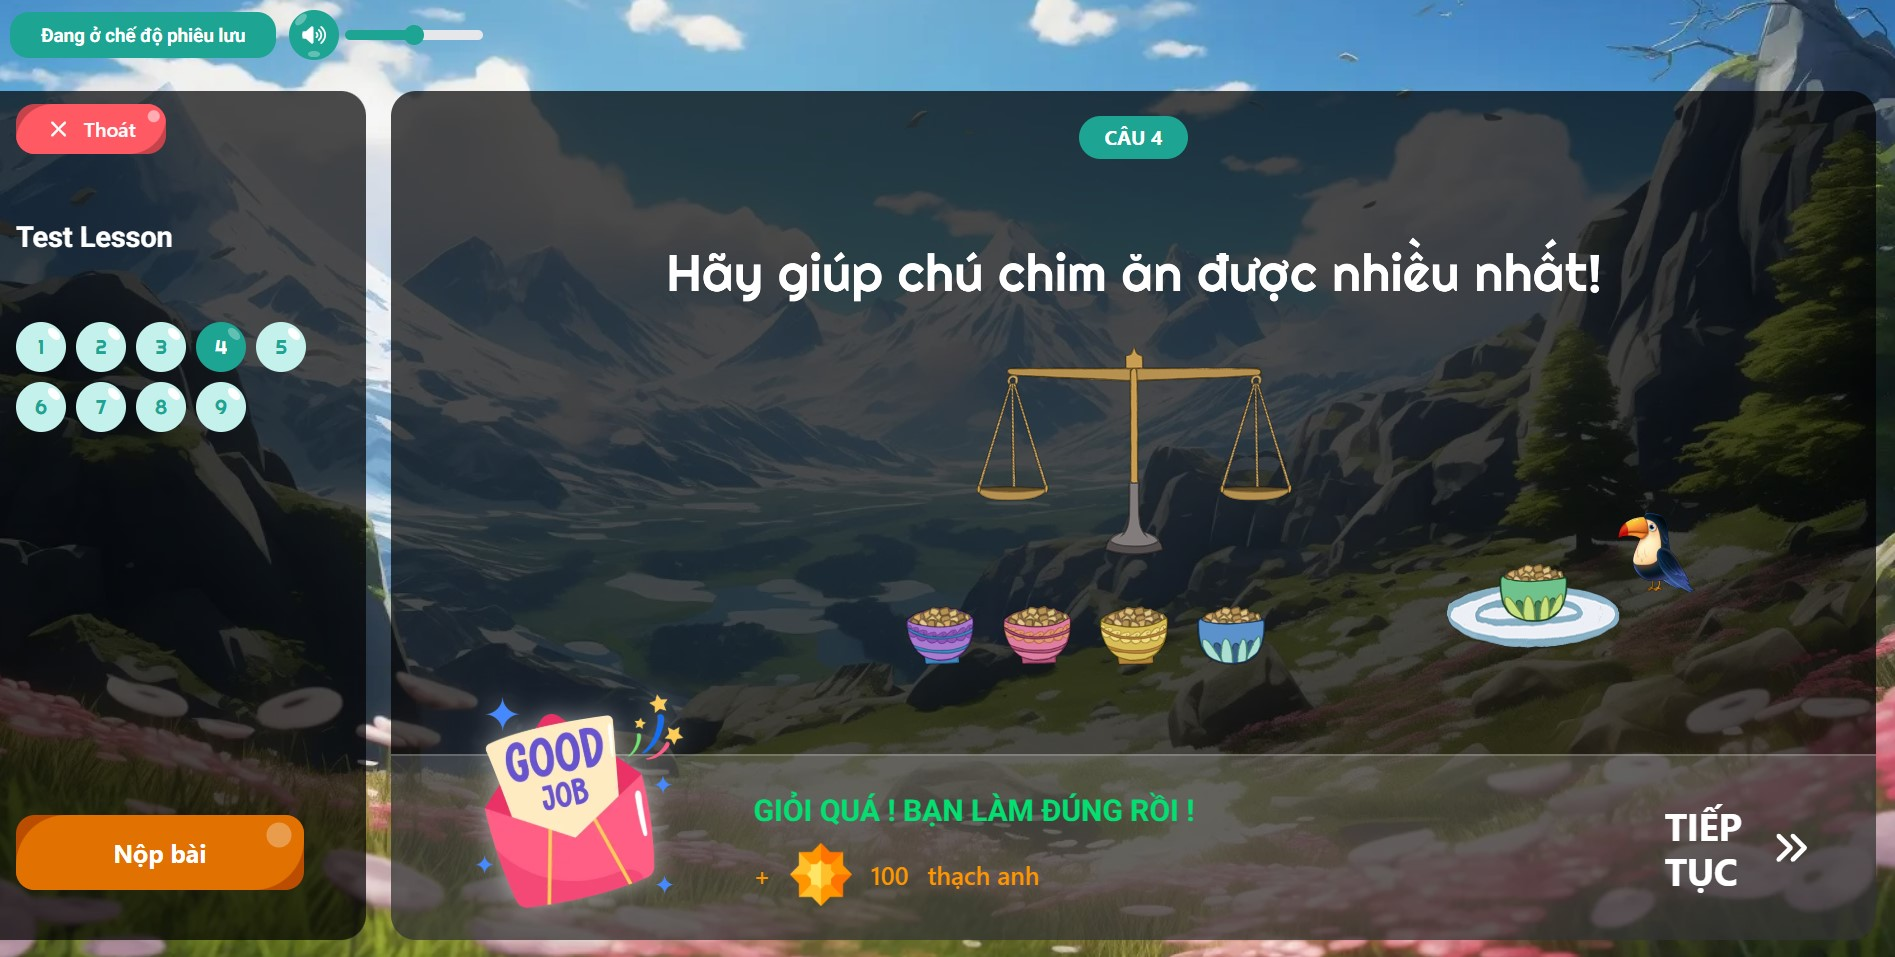
\includegraphics[width=0.9\textwidth]{Image/UI/Exercises/Correct.jpg}
	\vspace{0.6cm}
	\caption{Hiệu ứng chúc mừng khi làm đúng}
	\label{fig:correct}
\end{figure}
\begin{figure}[H]
	\centering
	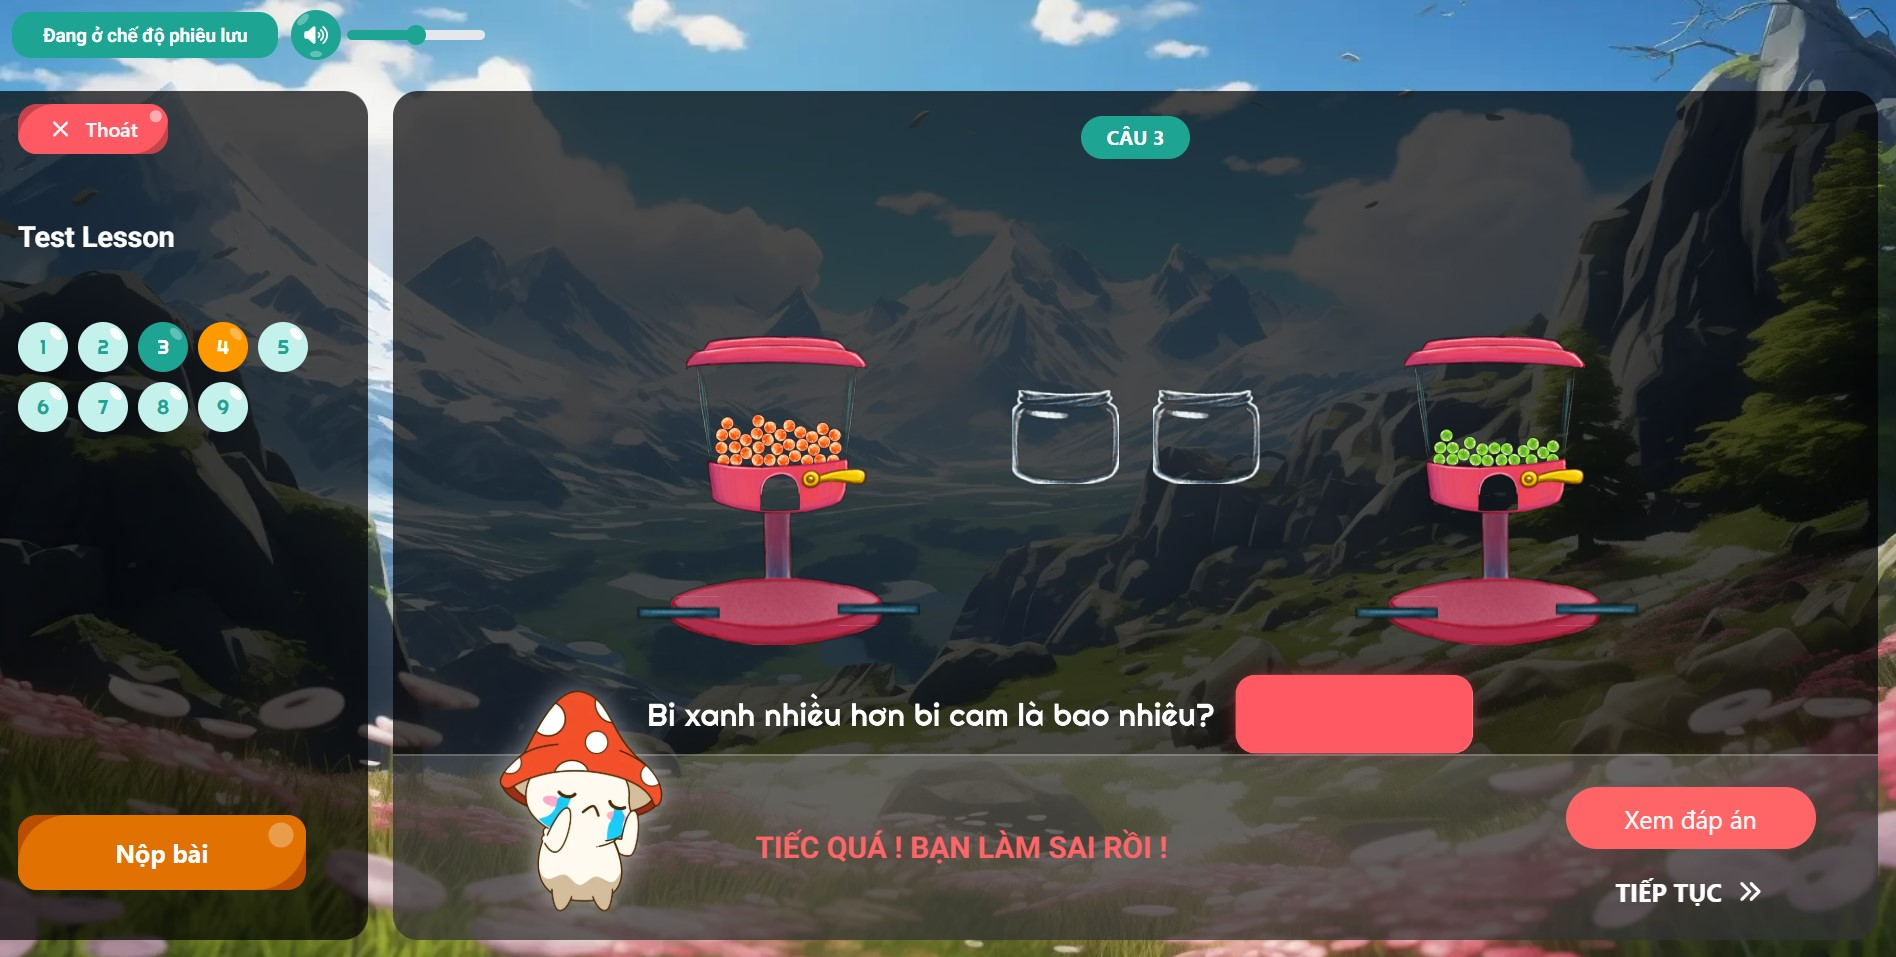
\includegraphics[width=\textwidth]{Image/UI/Exercises/Wrong.jpg}
	\vspace{0.6cm}
	\caption{Hiệu ứng chúc mừng khi làm đúng}
	\label{fig:wrong}
\end{figure}
\begin{figure}[H]
	\centering
	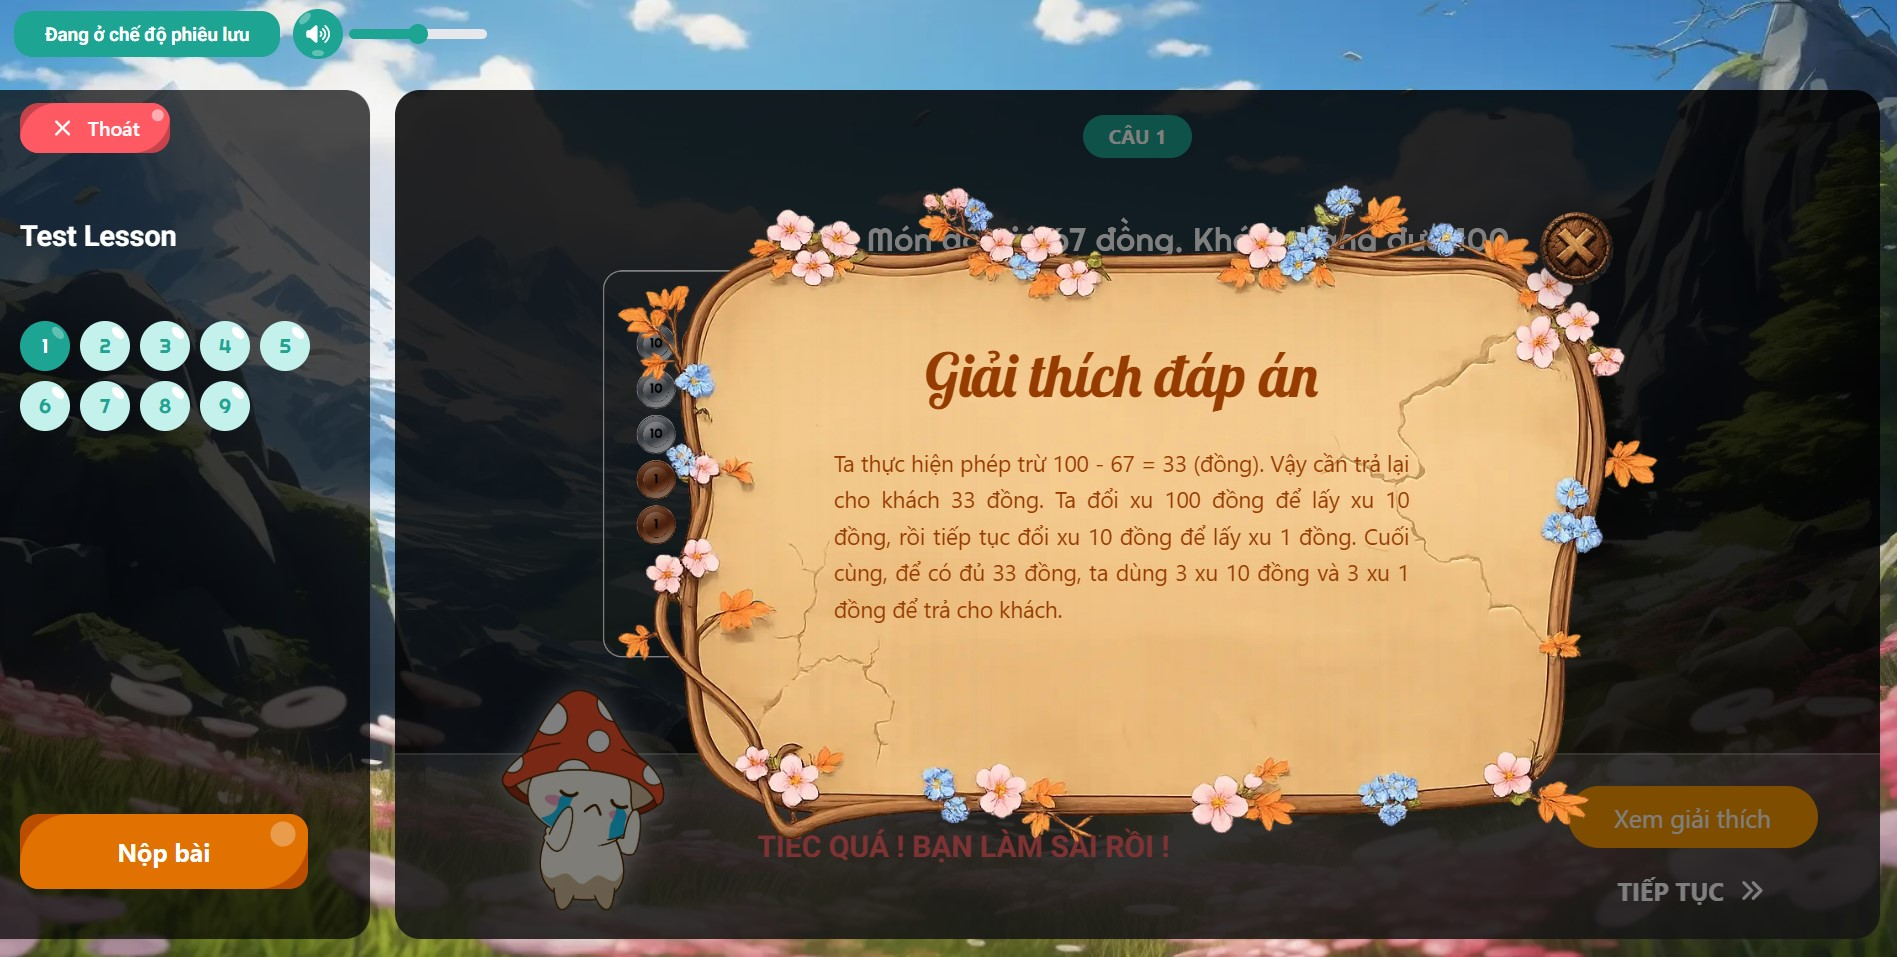
\includegraphics[width=\textwidth]{Image/UI/Exercises/Explain.jpg}
	\vspace{0.6cm}
	\caption{Xem giải thích đáp án khi làm sai}
	\label{fig:explain}
\end{figure}

Sau khi người dùng hoàn thành tất cả câu hỏi, giao diện kết quả sẽ được hiển thị như giao diện sẽ giống như \textit{Hình \ref{fig:result}} bao gồm tên lớp, chủ đề, tên bài học, tổng số điểm đạt được và tổng số thạch anh nhận được.
\begin{figure}[H]
	\centering
	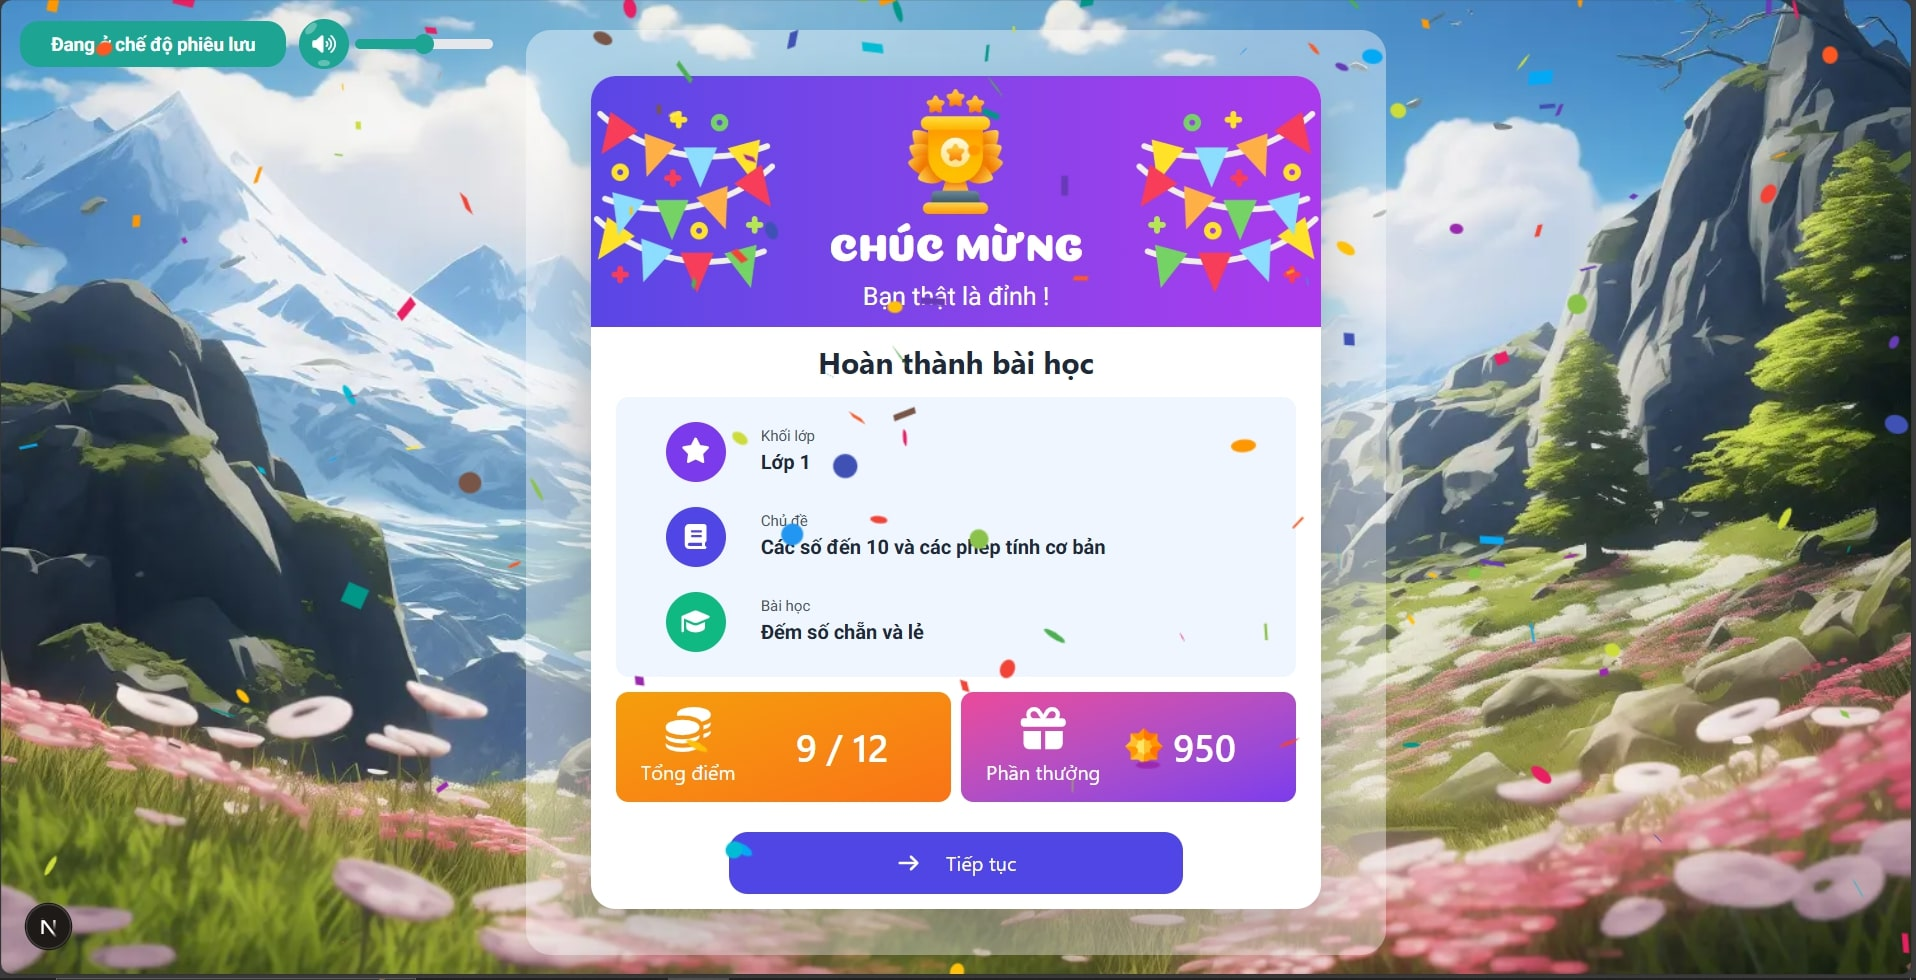
\includegraphics[width=0.9\textwidth]{Image/UI/Exercises/Finish.jpg}
	\vspace{0.6cm}
	\caption{Giao diện kết quả sau khi hoàn thành bài học}
	\label{fig:result}
\end{figure}

\subsubsection{Trang Đấu trường}
\label{subsubsec:arena}
Người dùng có thể tham gia làm bài thi đấu trường theo tuần, xem thời gian còn lại của đấu trường, xem bậc xếp hạng hiện tại của mình, xem bảng xếp hạng tuần và xem thể lệ đấu trường. Để bắt đầu làm bài thi, người dùng chỉ cần bấm nút \textit{Tham gia ngay} bên trong khung màu cam được hiển thị trên giao diện. Sau khi bấm nút, người dùng sẽ được điều hướng sang \textbf{Trang Bài thi} được mô tả ở mục \ref{subsubsec:exam}. Giao diện chính của trang đấu trường được thiết kế như \textit{Hình \ref{fig:arena}}.
\begin{figure}[H]
	\centering
	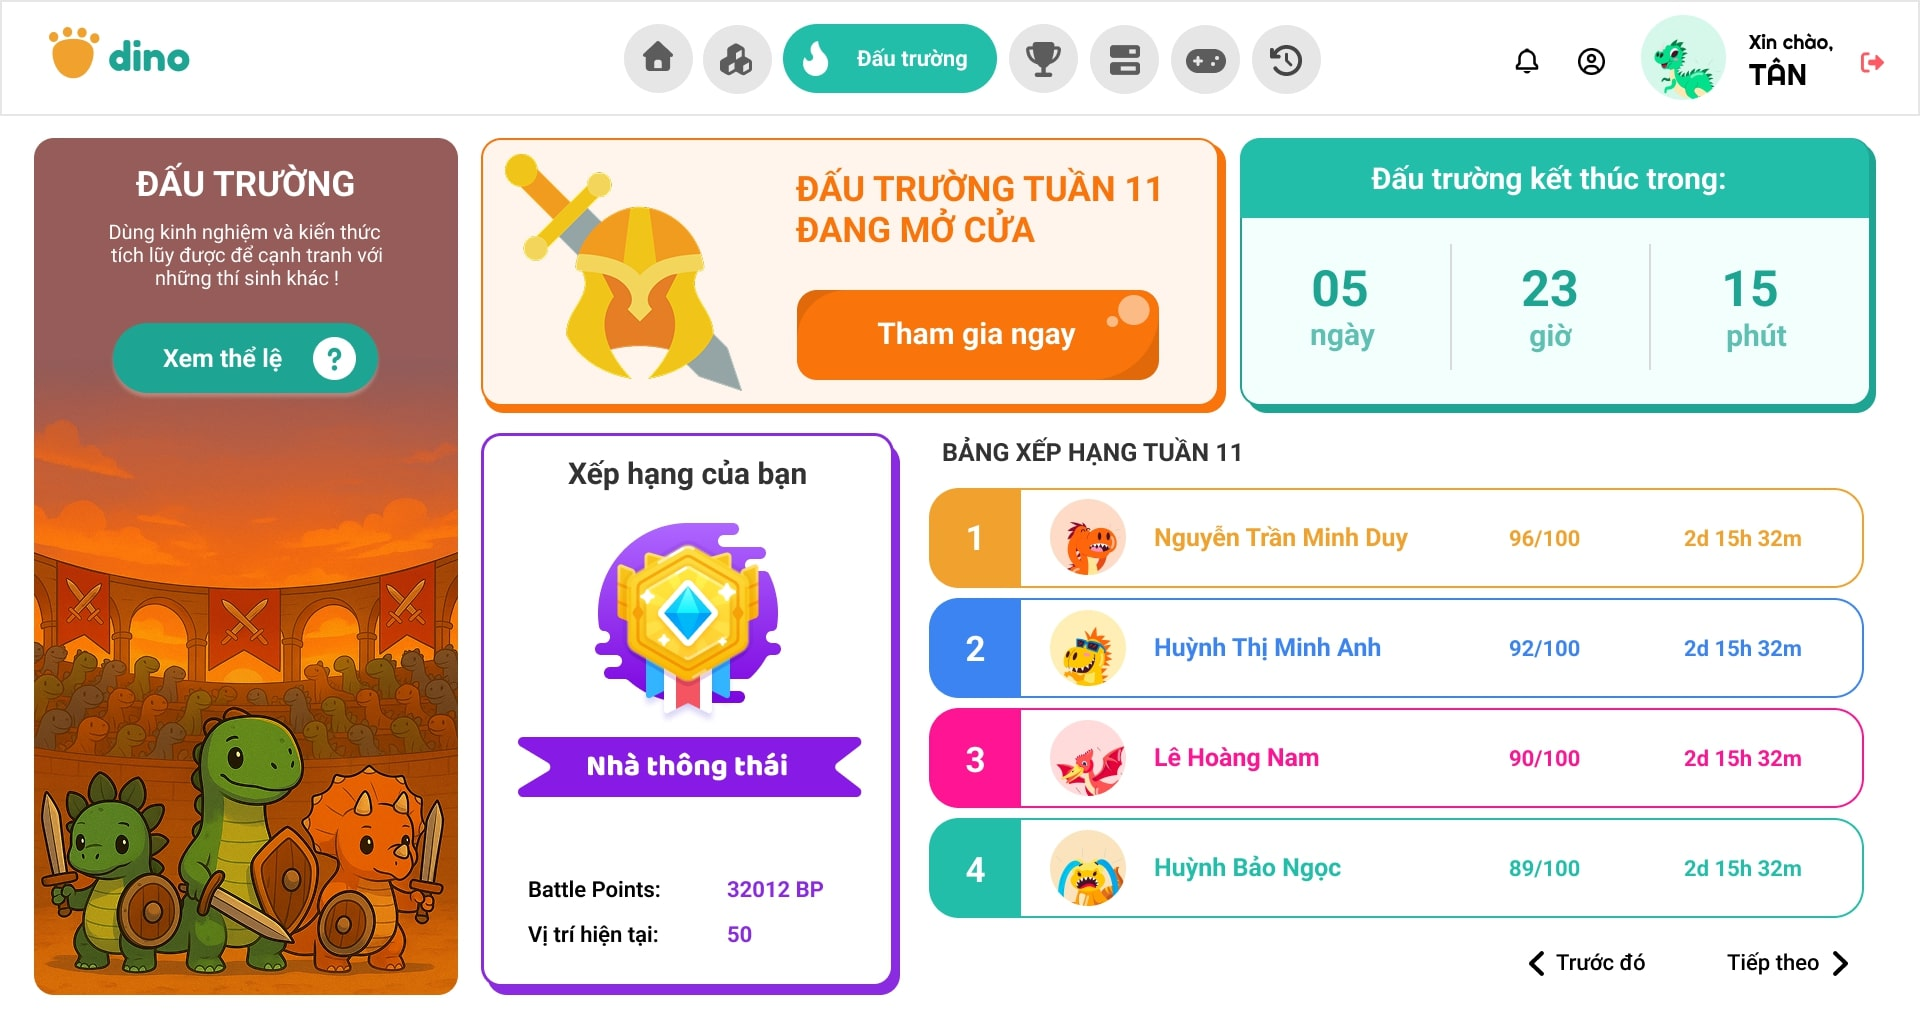
\includegraphics[width=0.9\textwidth]{Image/UI/Main-Student/Arena-Home.jpg}
	\vspace{0.6cm}
	\caption{Trang Đấu trường}
	\label{fig:arena}
\end{figure}

\vspace{0.2cm}
\newline
Để xem thể lệ cuộc thi, người dùng bấm vào nút \textit{Xem thể lệ} nằm ở bên trái của giao diện. Trang thể lệ đấu trường sẽ được phóng to, người dùng có thể bấm chuyển trang để đọc hết tất cả các thể lệ.
\begin{figure}[H]
	\centering
	\begin{minipage}{1.0\textwidth} % Sử dụng toàn bộ độ rộng văn bản
		\centering
		
		% Dòng 1
		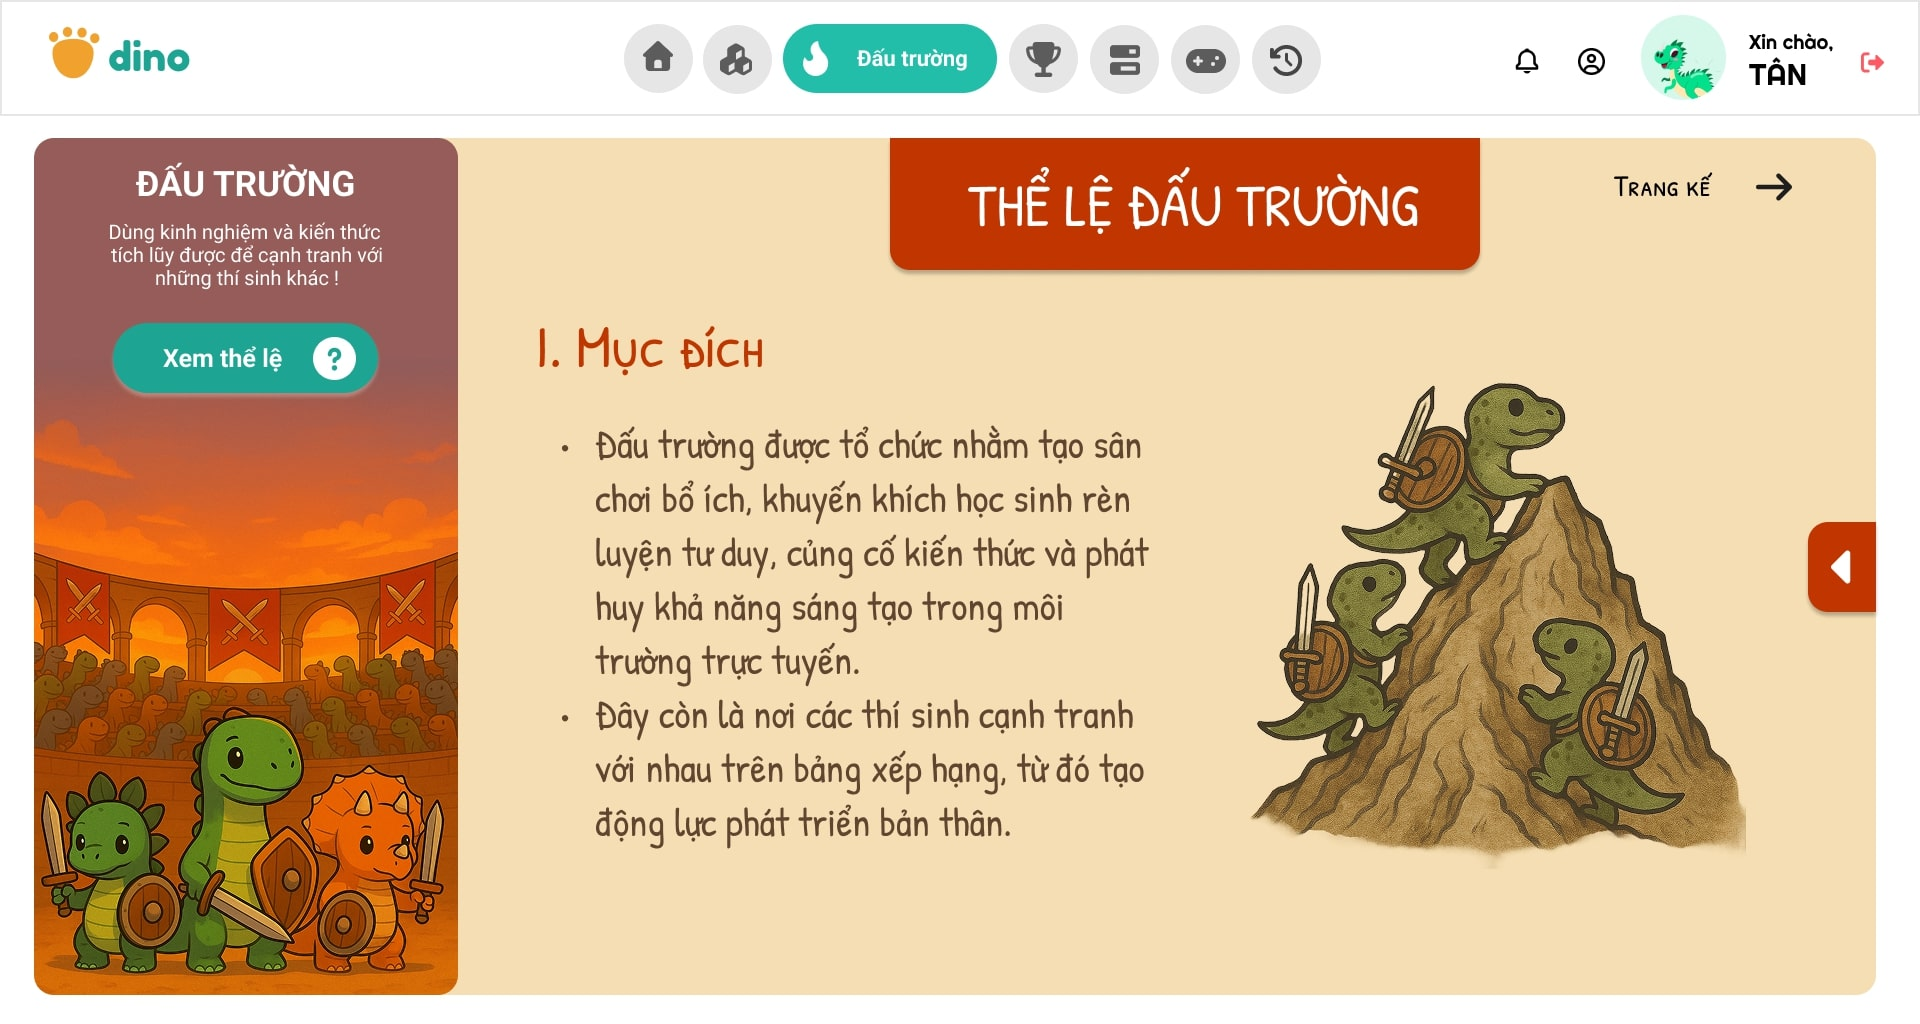
\includegraphics[width=0.48\textwidth]{Image/UI/Main-Student/Arena-R1.jpg}
		\hspace{0.1cm} % Đẩy hình 2 sang sát lề phải của minipage
		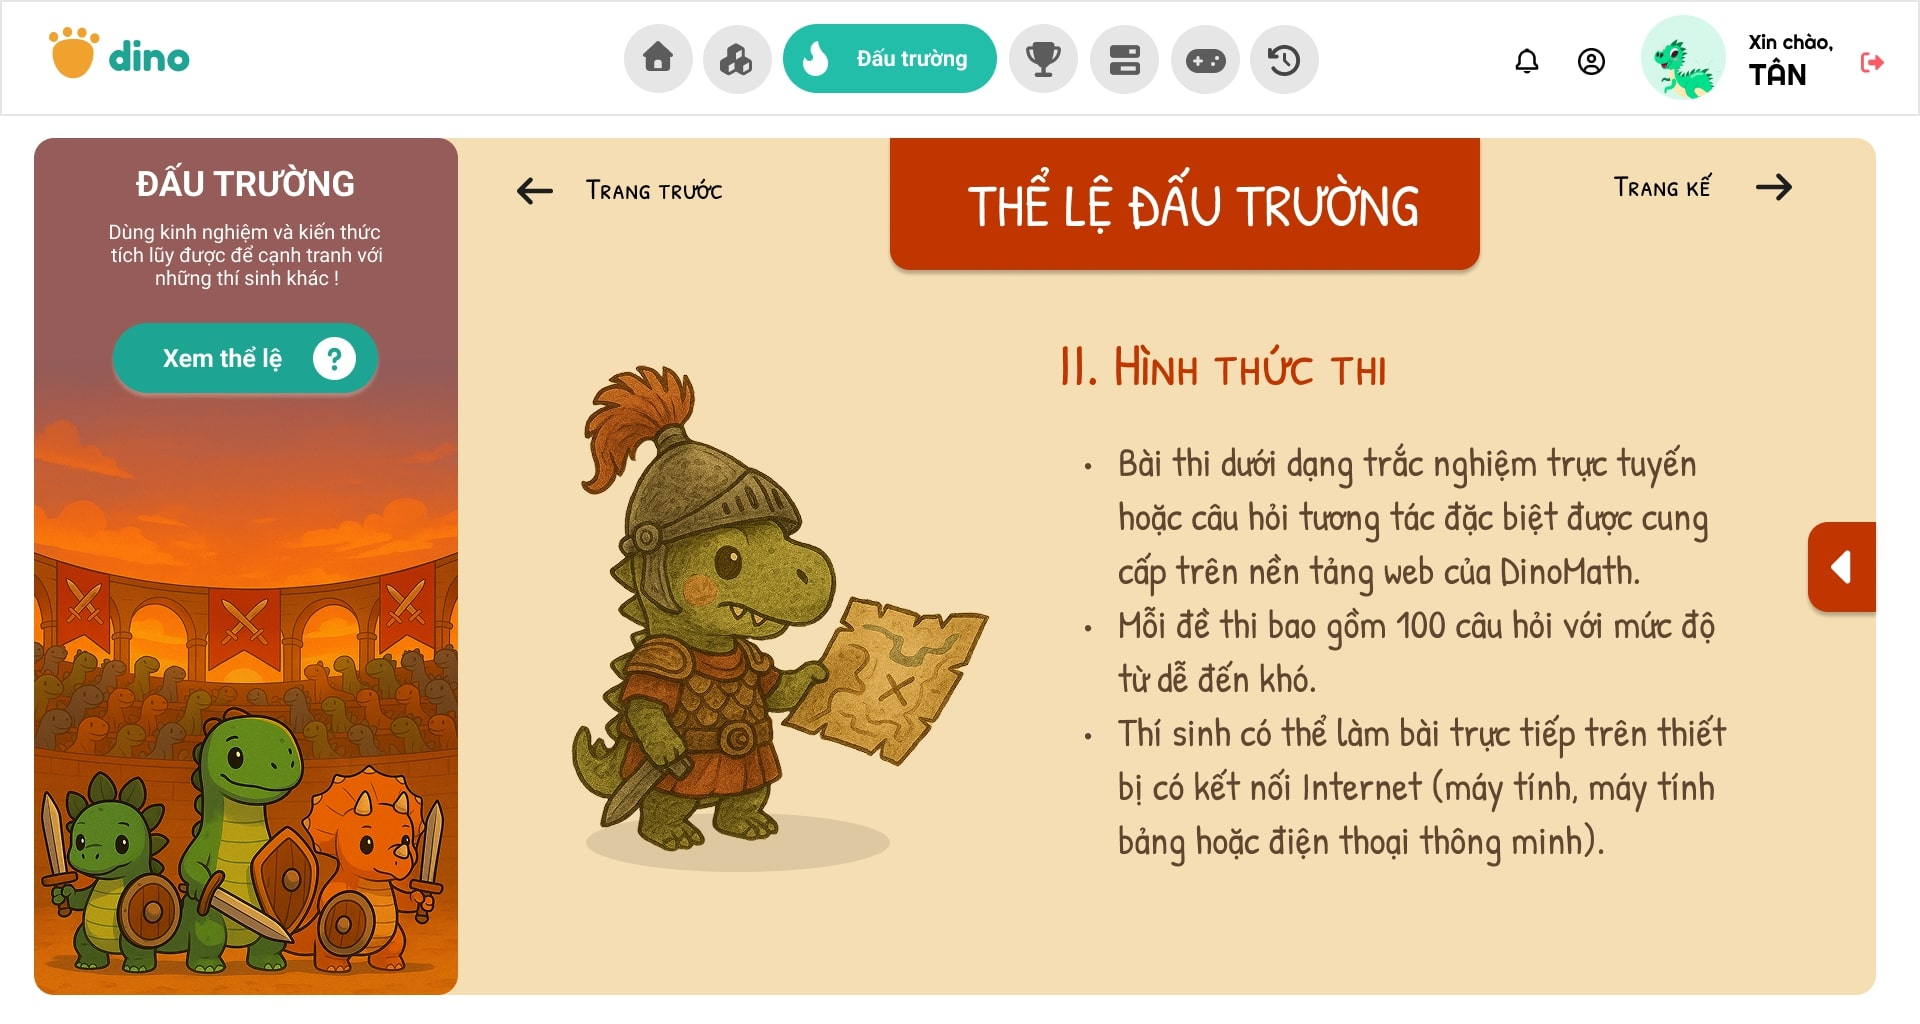
\includegraphics[width=0.48\textwidth]{Image/UI/Main-Student/Arena-R2.jpg}
		\\[0.3cm] % Khoảng cách dòng
		
		% Dòng 2
		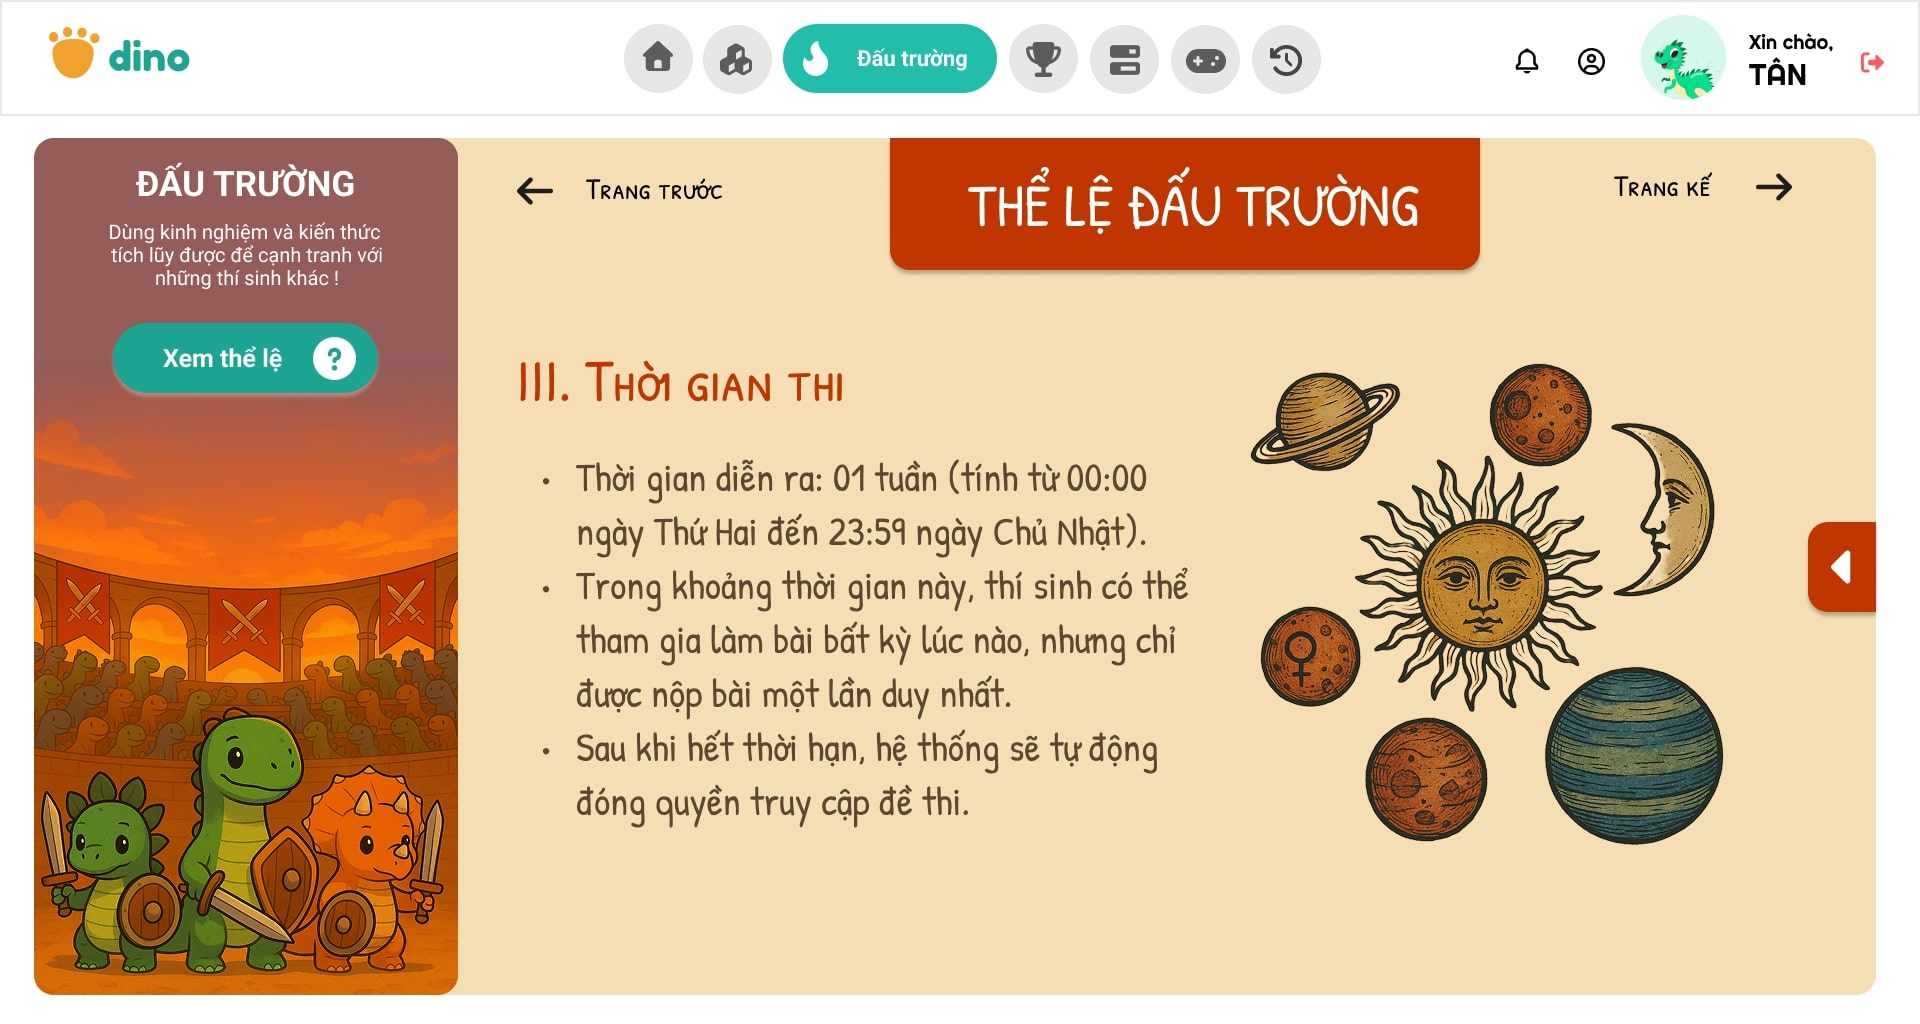
\includegraphics[width=0.48\textwidth]{Image/UI/Main-Student/Arena-R3.jpg}
		\hspace{0.1cm}
		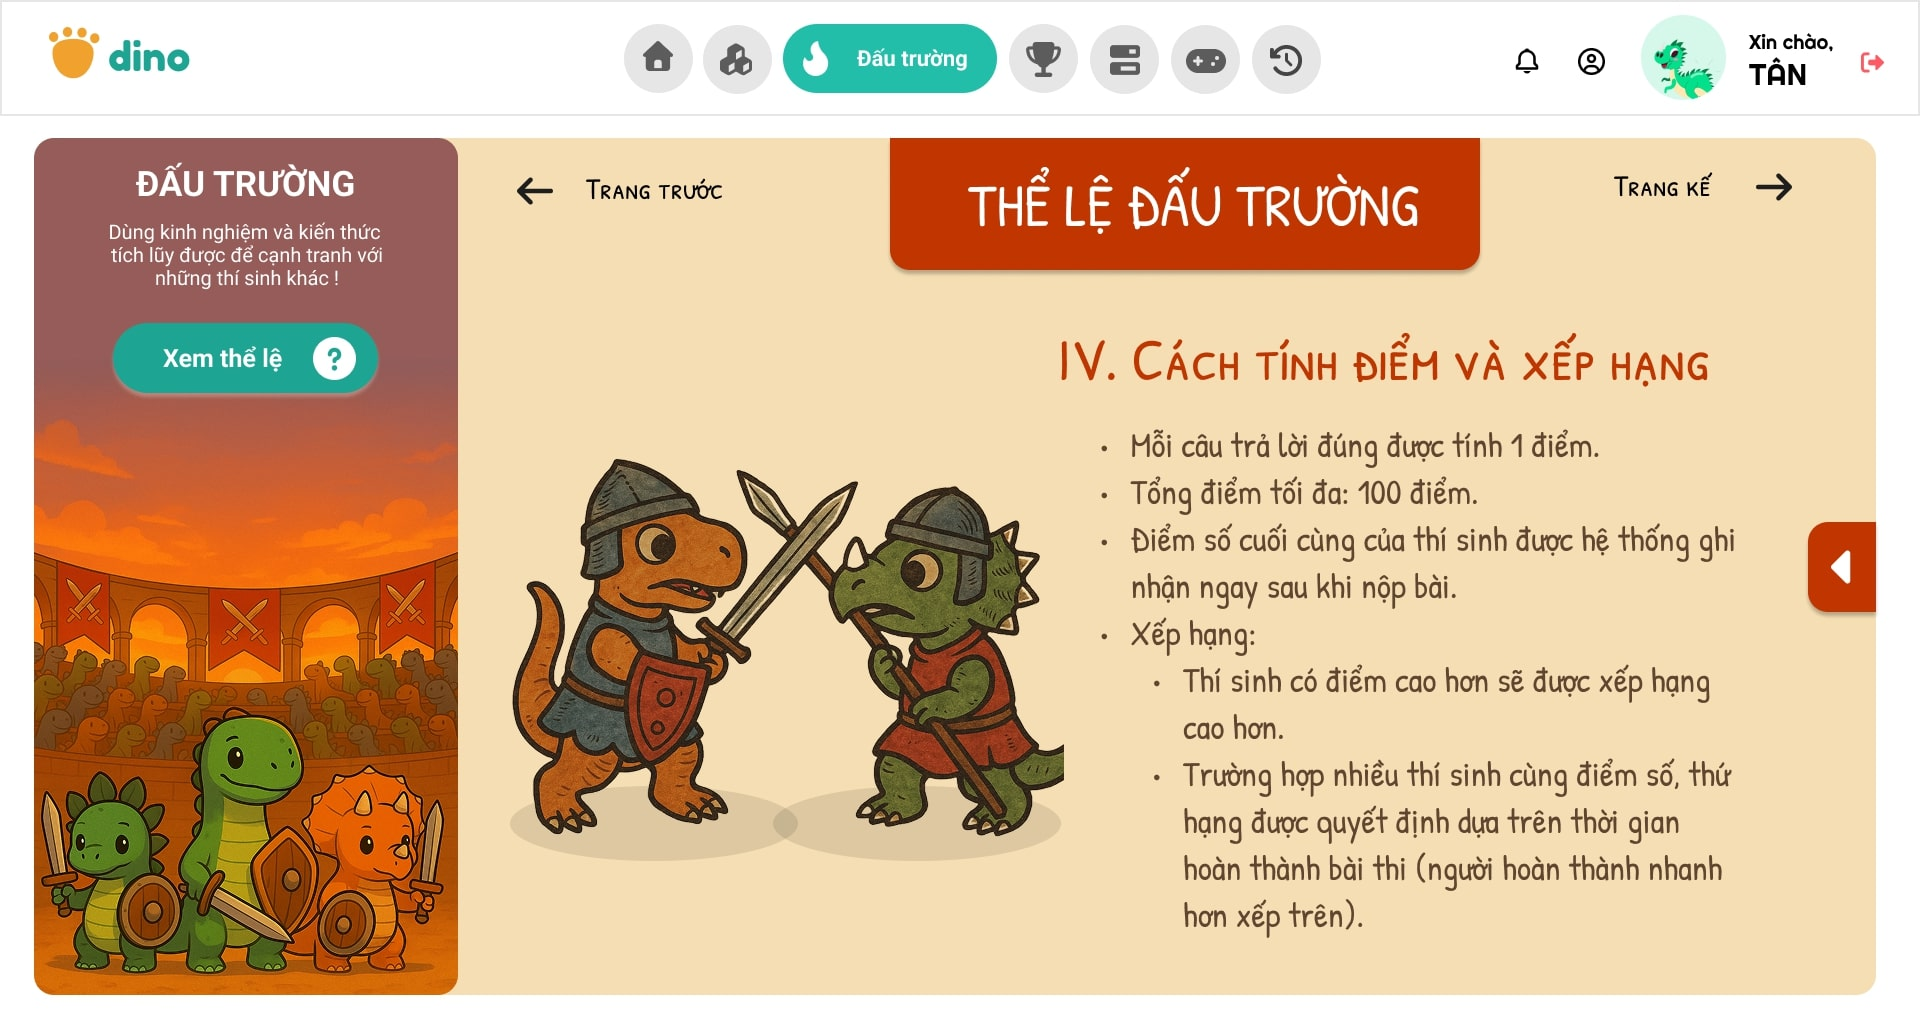
\includegraphics[width=0.48\textwidth]{Image/UI/Main-Student/Arena-R4.jpg}
		\\[0.3cm]
		
		% Dòng 3 (Hình cuối cùng nằm giữa hoặc căn trái tùy ý)
		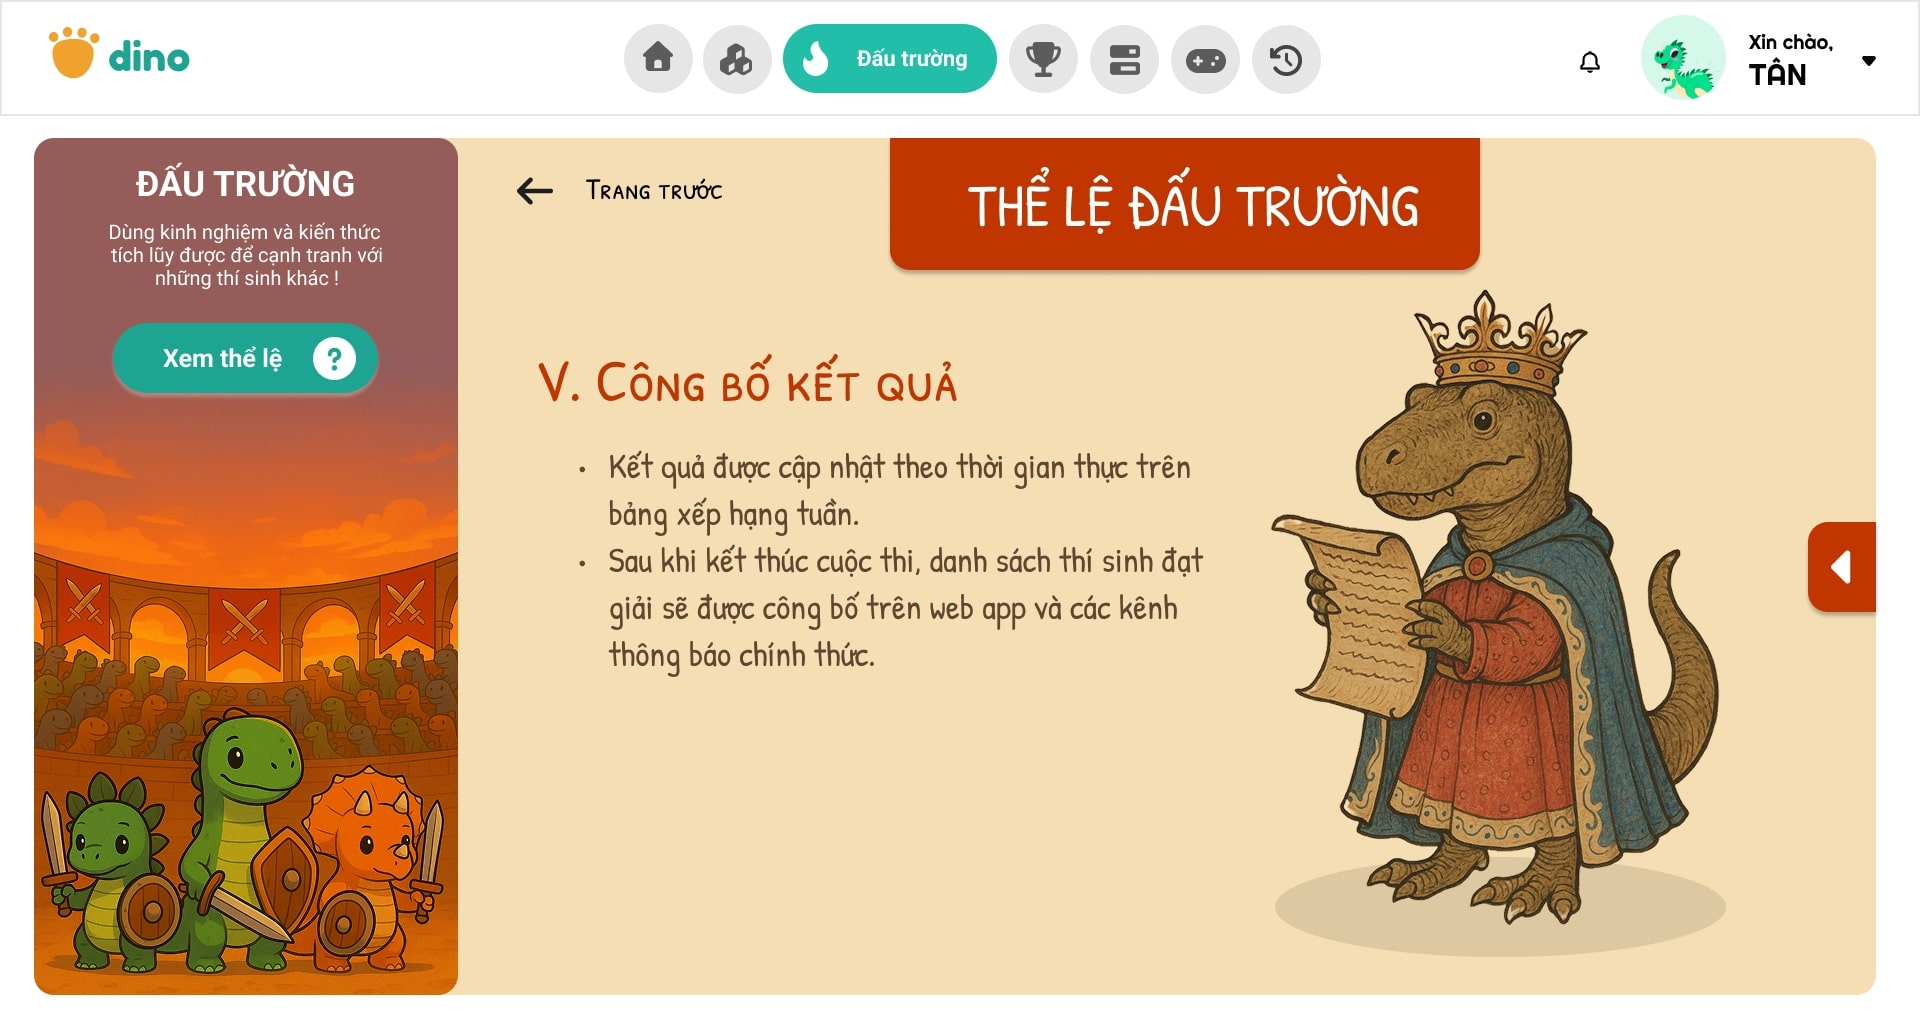
\includegraphics[width=0.48\textwidth]{Image/UI/Main-Student/Arena-R5.jpg}
		
	\end{minipage}
	\vspace{0.4cm}
	\caption{Trang Đấu trường - Thể lệ}
	\label{fig:arena-rules}
\end{figure}

Sau khi có kết quả bài thi Đấu trường, tùy theo số điểm đạt được mà mỗi thí sinh sẽ được thưởng một lượng Battle Points nhất định (đơn vị điểm dành riêng cho đấu trường). Battle Points (BP) sẽ là tiêu chí để xét xem một người dùng đang ở bậc xếp hạng nào. Các bậc xếp hạng và huy hiệu tương ứng được thiết kế như \textit{Hình \ref{fig:badges}}. Đối với bảng xếp hạng tuần, thứ hạng được quyết định dựa trên số điểm đạt được và thời gian hoàn thành bài thi của mỗi thí sinh.
	\begin{figure}[H]
		\centering
		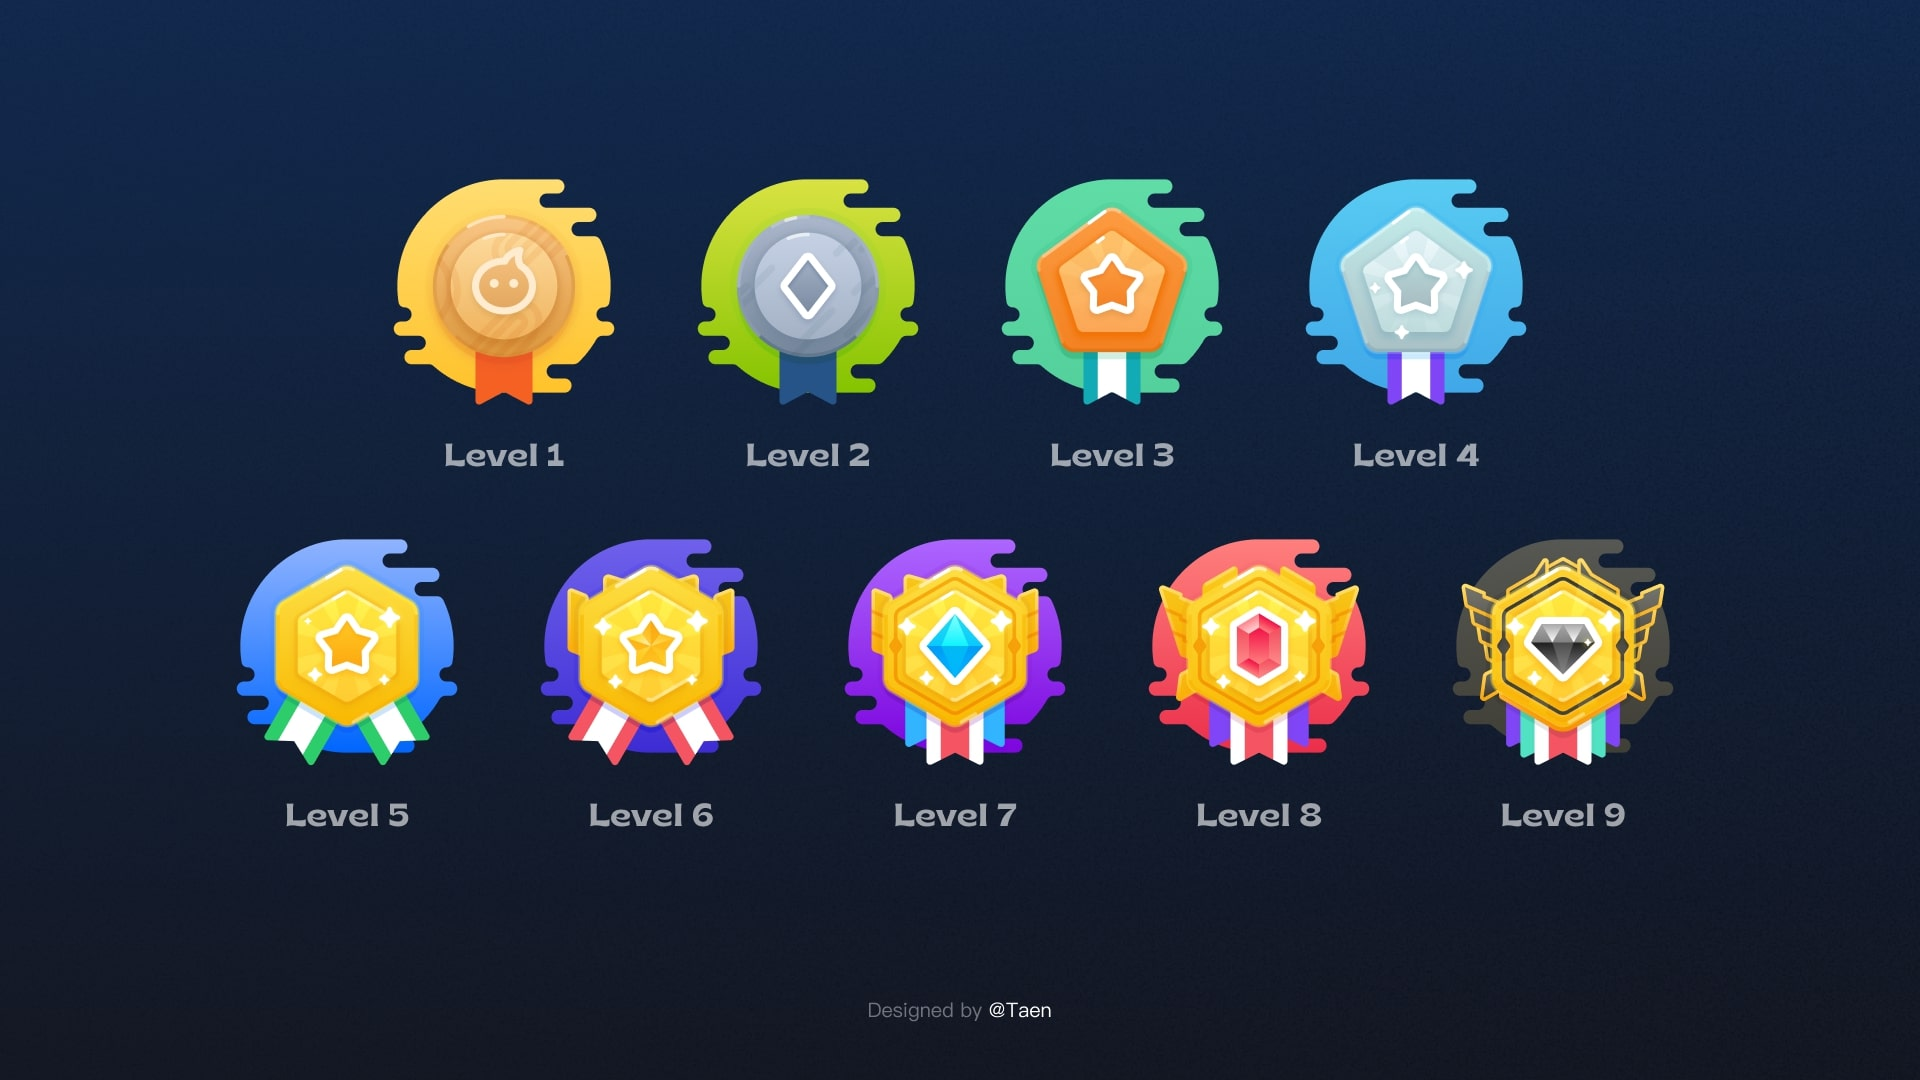
\includegraphics[width=0.9\textwidth]{Image/UI/badges.jpg}
		\vspace{0.6cm}
		\caption[
		Hệ thống các huy hiệu ứng với từng bậc xếp hạng
		]{
			\centering
			Hệ thống các huy hiệu ứng với từng bậc xếp hạng \\
			\textit{(nguồn: Rank Badge Design - Free by Taen \cite{figma_community_file})}
		}
		\label{fig:badges}
	\end{figure}
	
	
	\begin{figure}[H]
		\centering
		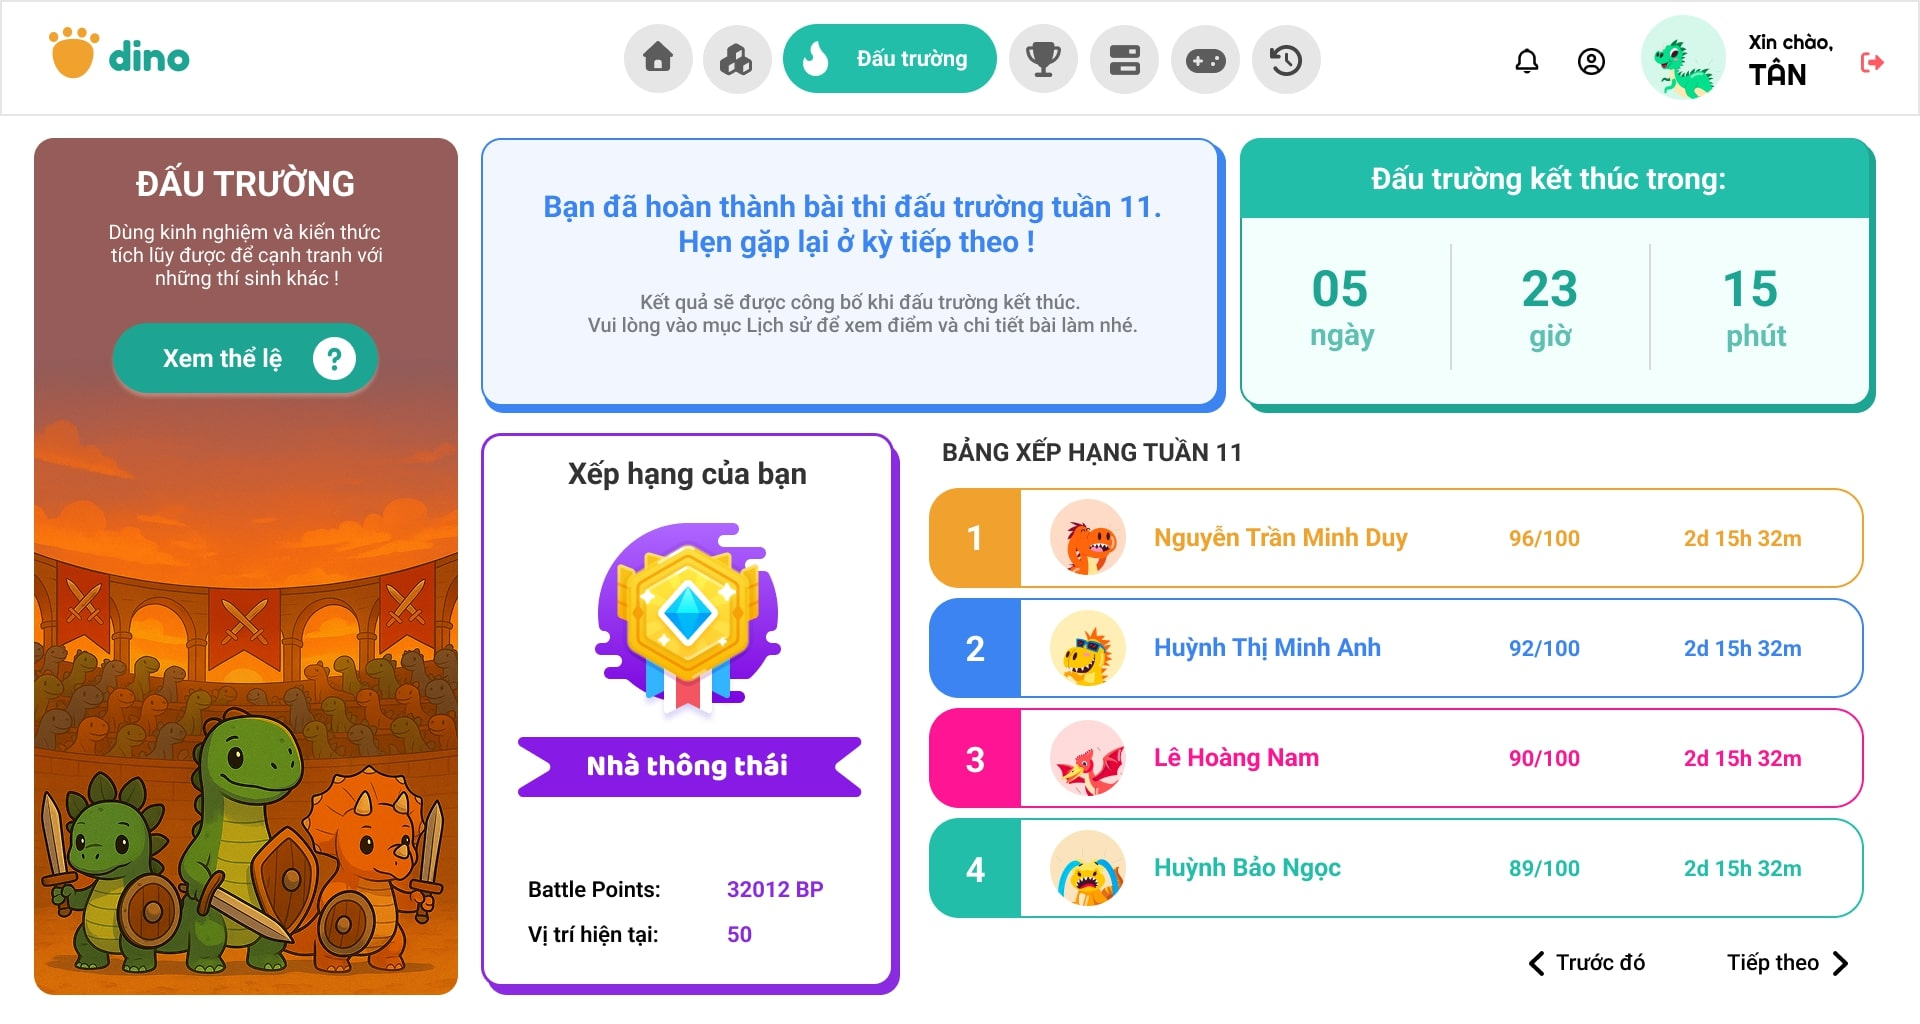
\includegraphics[width=0.9\textwidth]{Image/UI/Main-Student/Arena-Finished.jpg}
		\vspace{0.6cm}
		\caption{Trang Đấu trường - Sau khi hoàn thành bài thi}
	\end{figure}
\end{itemize}

\subsubsection{Trang Bài thi}
\label{subsubsec:exam}
\textbf{Trang Bài thi} cung cấp giao diện làm bài cho \textbf{Bài kiểm tra đầu vào} (mục \ref{subsubsec:studenthome}) và \textbf{Đấu trường} (mục \ref{subsubsec:arena}). Người dùng có thể chuyển câu hỏi bằng cách bấm vào các nút số ở thanh bên trái của màn hình hoặc bấm các nút điều hướng để chuyển sang câu tiếp theo hoặc trước đó. Giao diện còn hỗ trợ hiển thị thời gian làm bài còn lại cũng như số câu hỏi đã làm trên tổng số câu hỏi. Tất cả các câu hỏi kiểm tra sẽ thuộc dạng trắc nghiệm. Đối với bài thi Đấu trường, do thời gian làm bài dài (7 ngày), người dùng có thể thoát và lưu tiến trình làm bài của mình để có thể tiếp tục làm sau đó.
	\begin{figure}[H]
		\centering
		\begin{minipage}{0.45\textwidth}
			\centering
			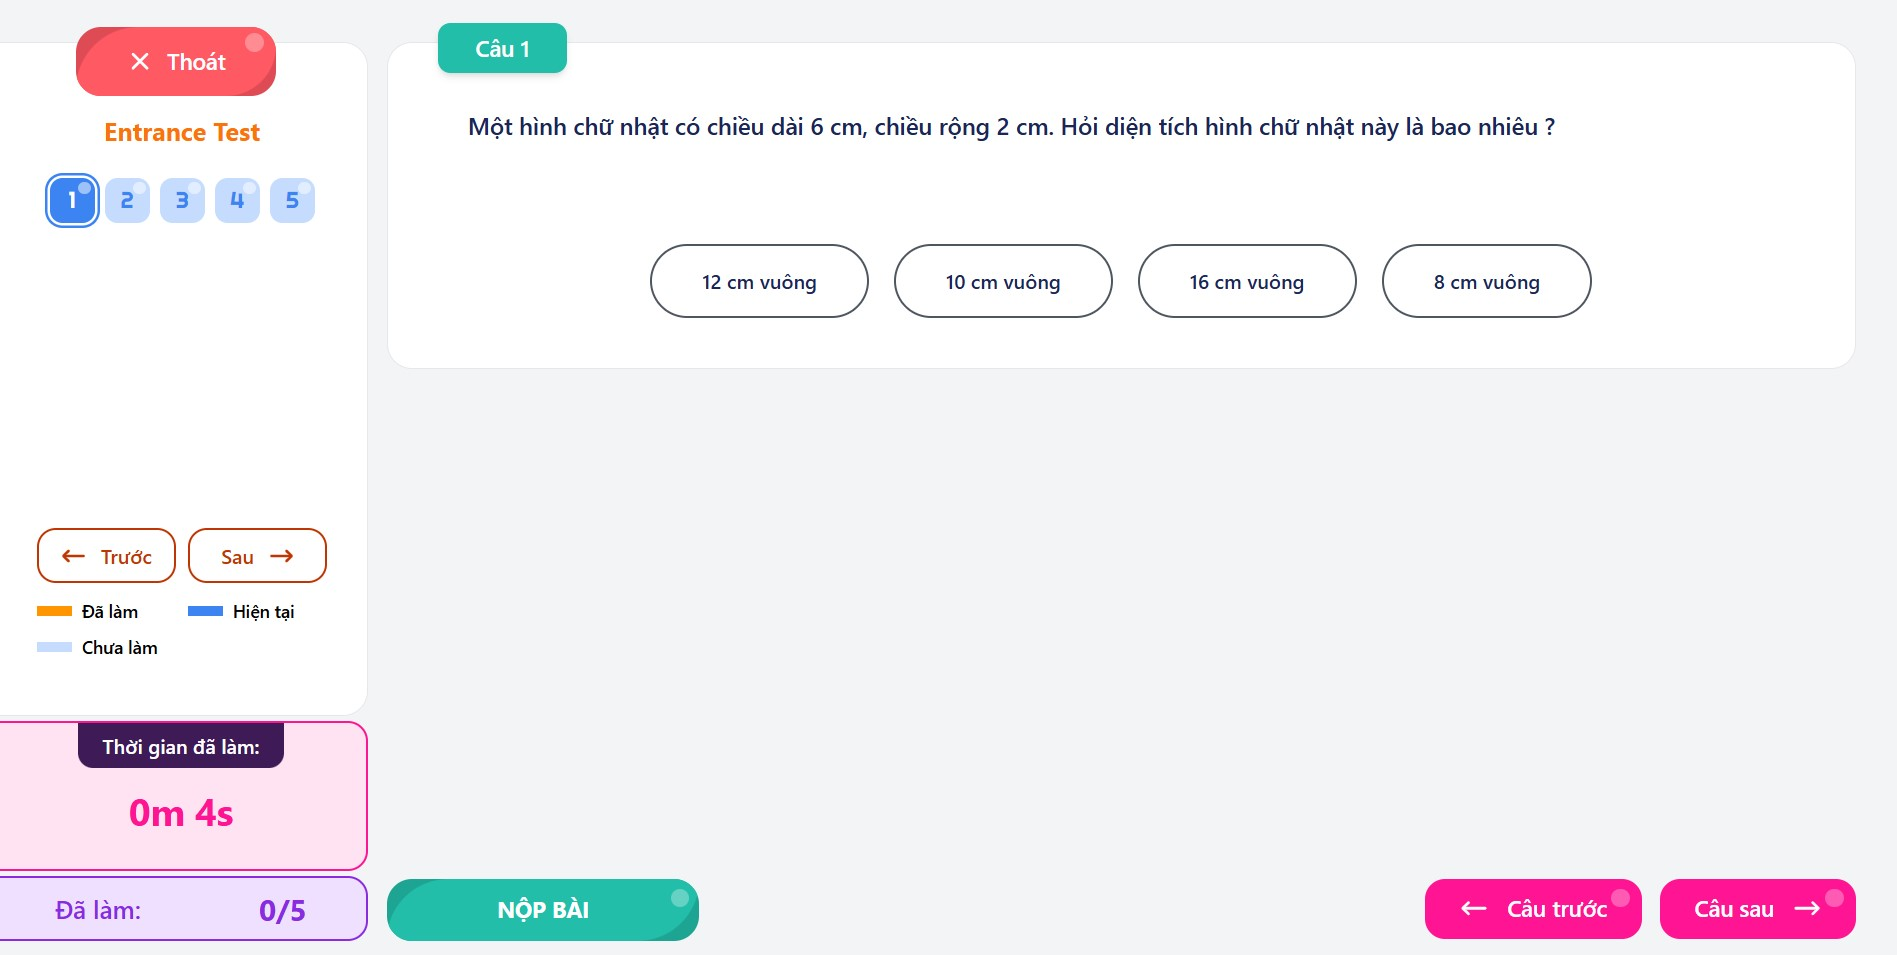
\includegraphics[width=\textwidth]{Image/UI/Main-Student/ExamChoices.jpg}
			\vspace{0.2cm}
			\caption{Dạng trắc nghiệm}
			\label{fig:exam1}
		\end{minipage}
		\hspace{0.1cm}
		\begin{minipage}{0.45\textwidth}
			\centering
			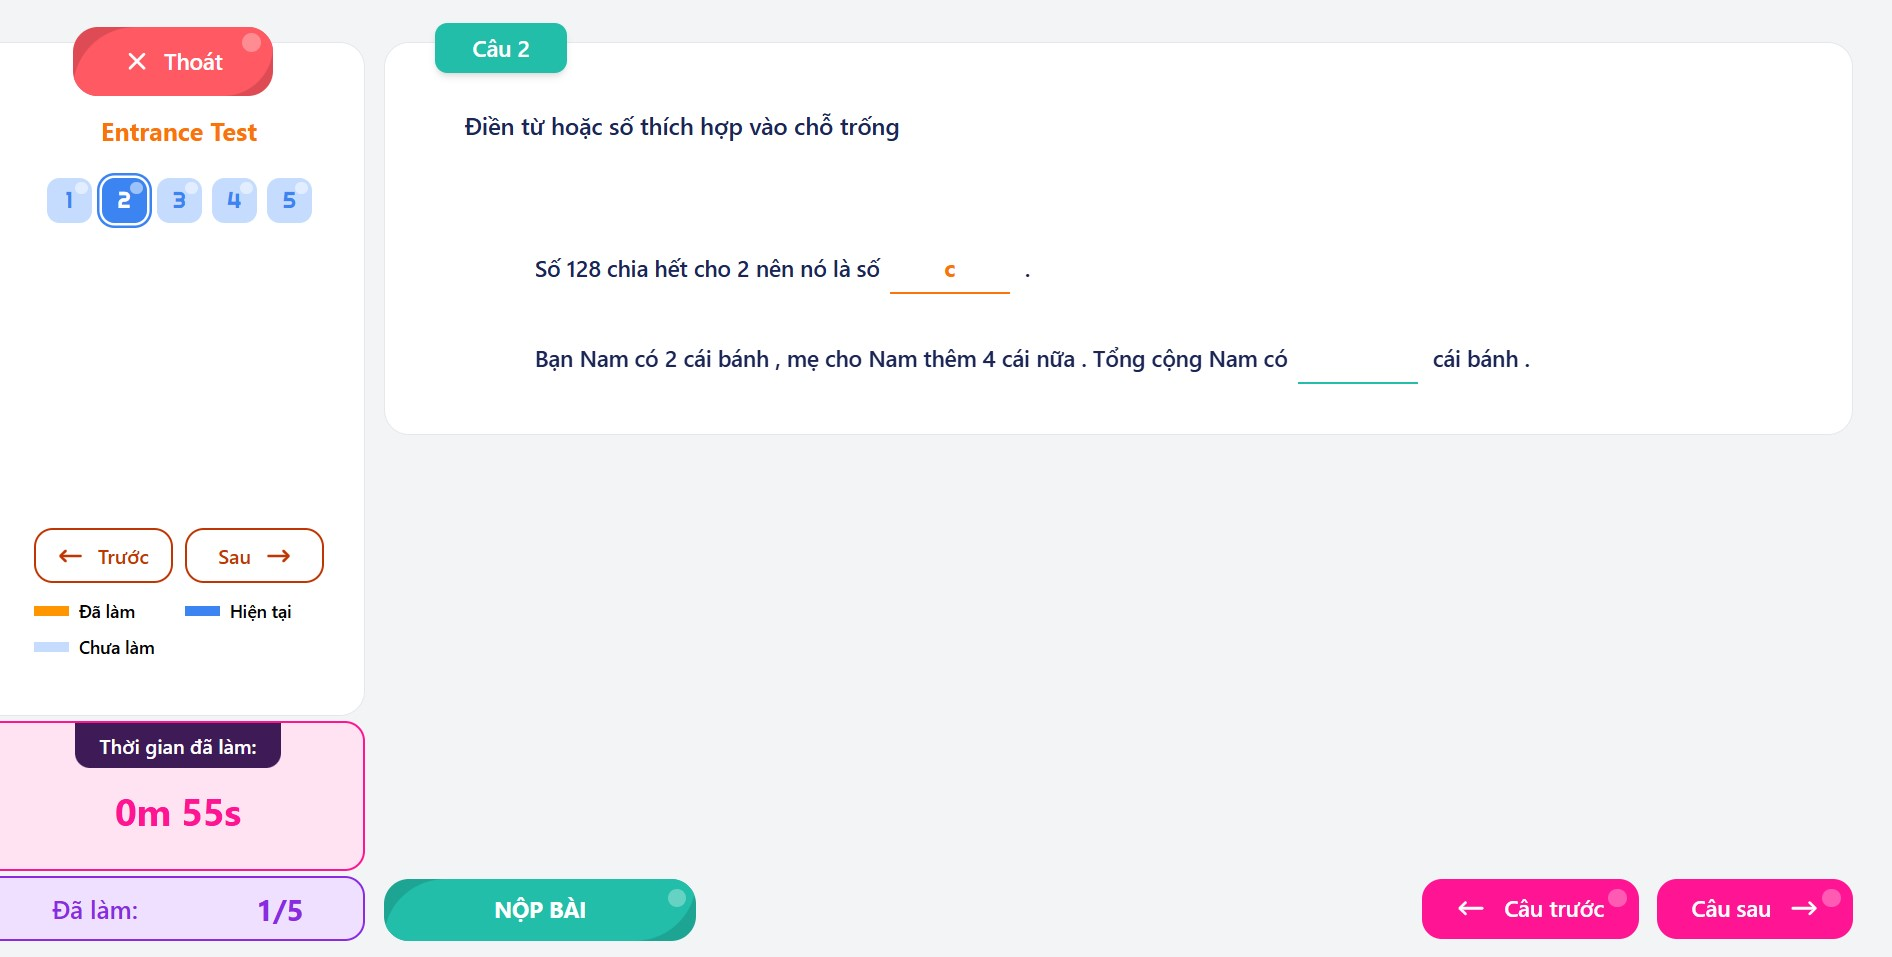
\includegraphics[width=\textwidth]{Image/UI/Main-Student/ExamFill.jpg}
			\vspace{0.2cm}
			\caption{Dạng điền khuyết}
			\label{fig:exam2}
		\end{minipage}
		
		\vspace{0.4cm}
		
		\begin{minipage}{0.45\textwidth}
			\centering
			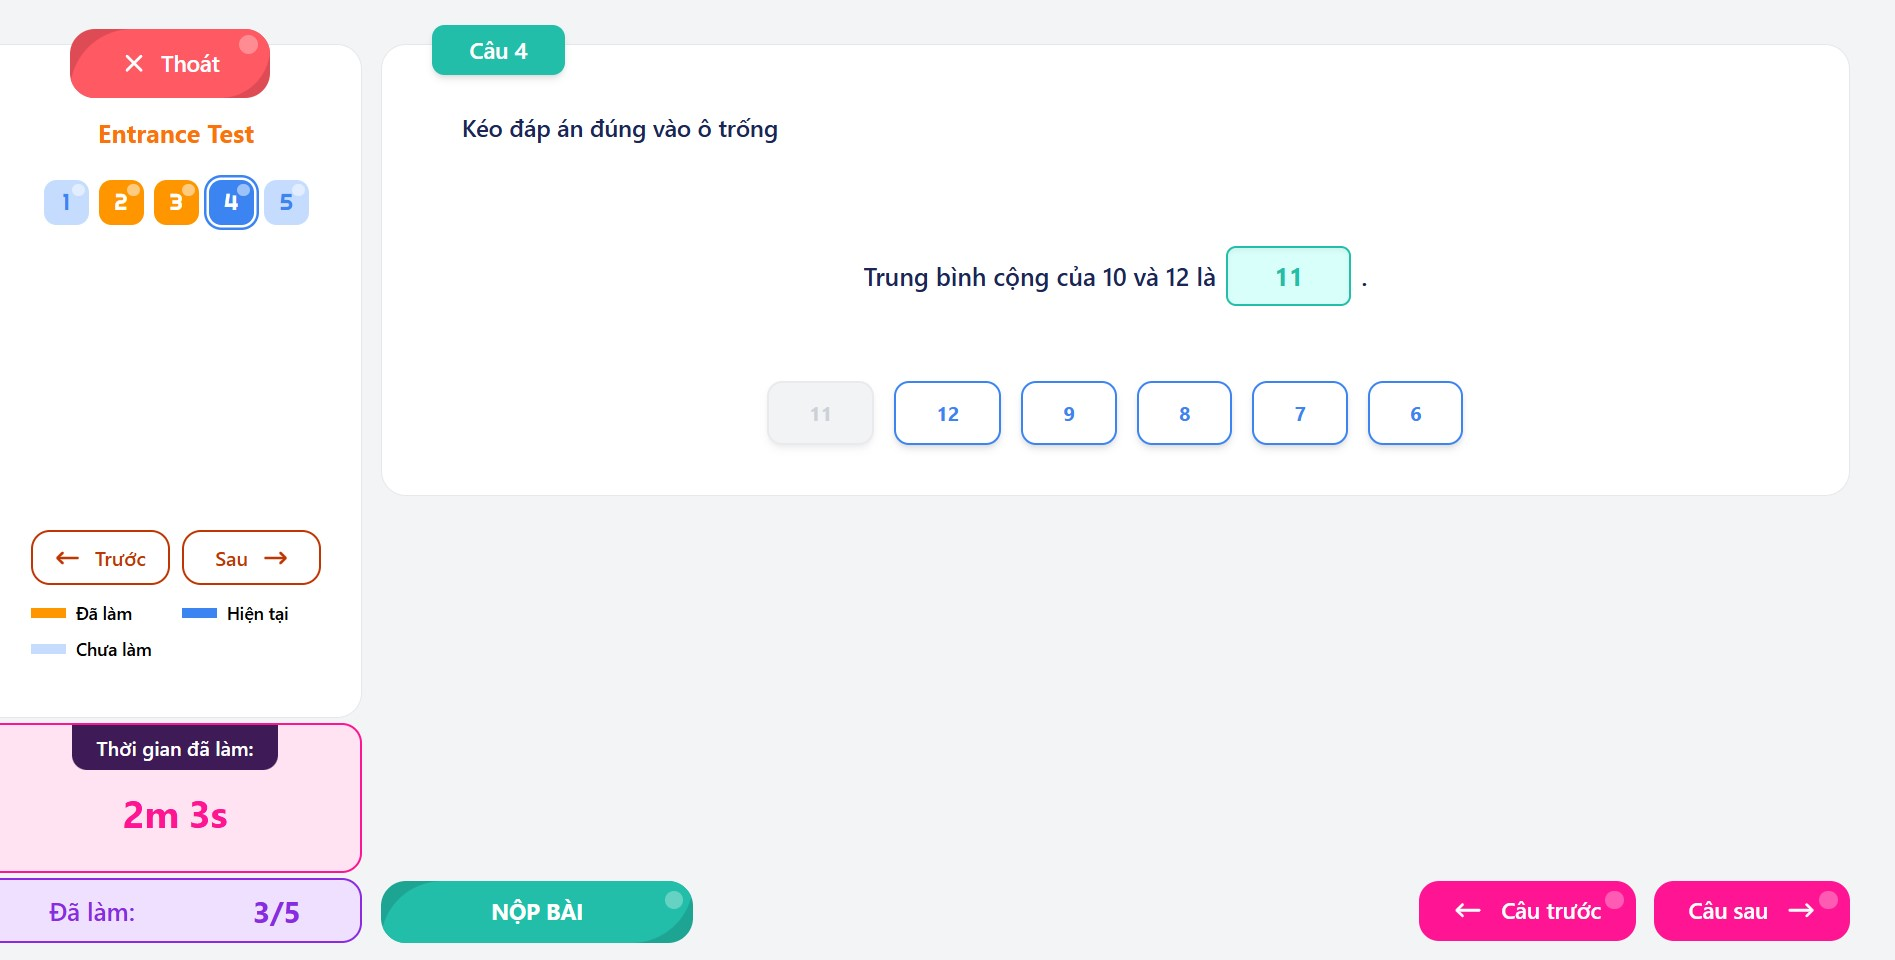
\includegraphics[width=\textwidth]{Image/UI/Main-Student/ExamFill2.jpg}
			\vspace{0.2cm}
			\caption{Dạng điền khuyết - Click to Fill}
			\label{fig:exam3}
		\end{minipage}
		\hspace{0.1cm}
		\begin{minipage}{0.45\textwidth}
			\centering
			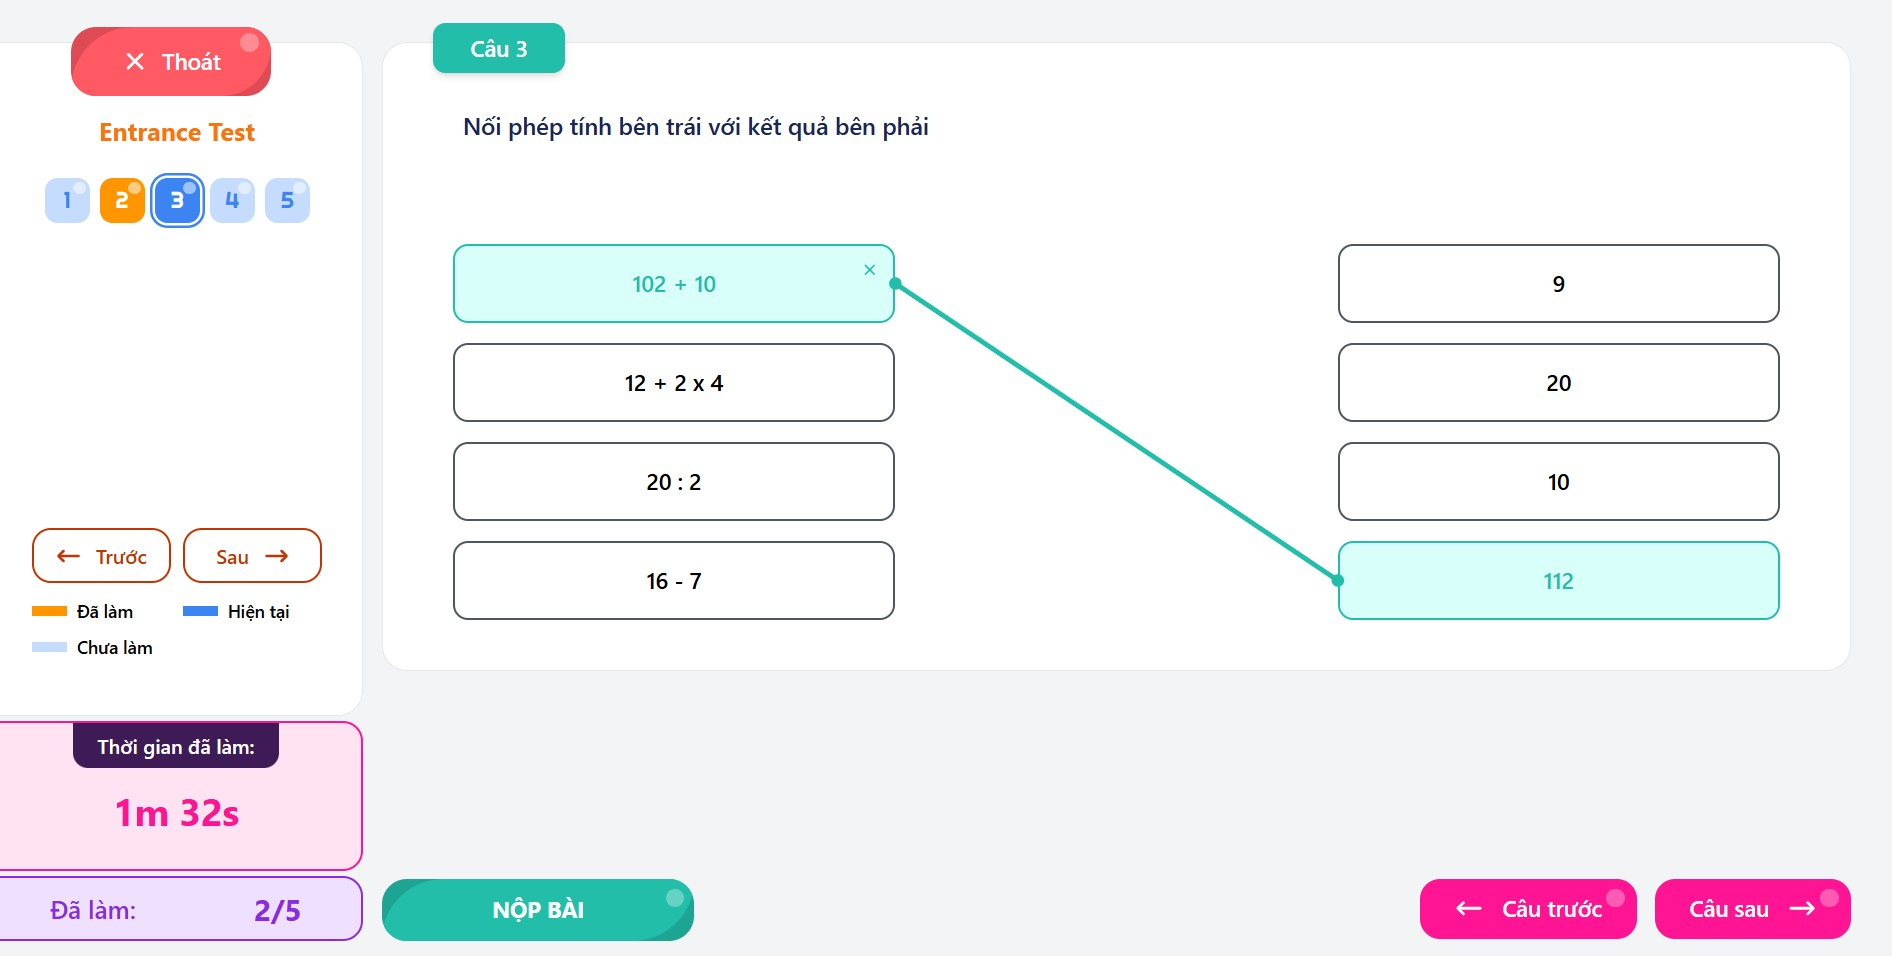
\includegraphics[width=\textwidth]{Image/UI/Main-Student/ExamMatching.jpg}
			\vspace{0.2cm}
			\caption{Dạng nối}
			\label{fig:exam4}
		\end{minipage}
		
		\vspace{0.4cm}
		
		\begin{minipage}{0.45\textwidth}
			\centering
			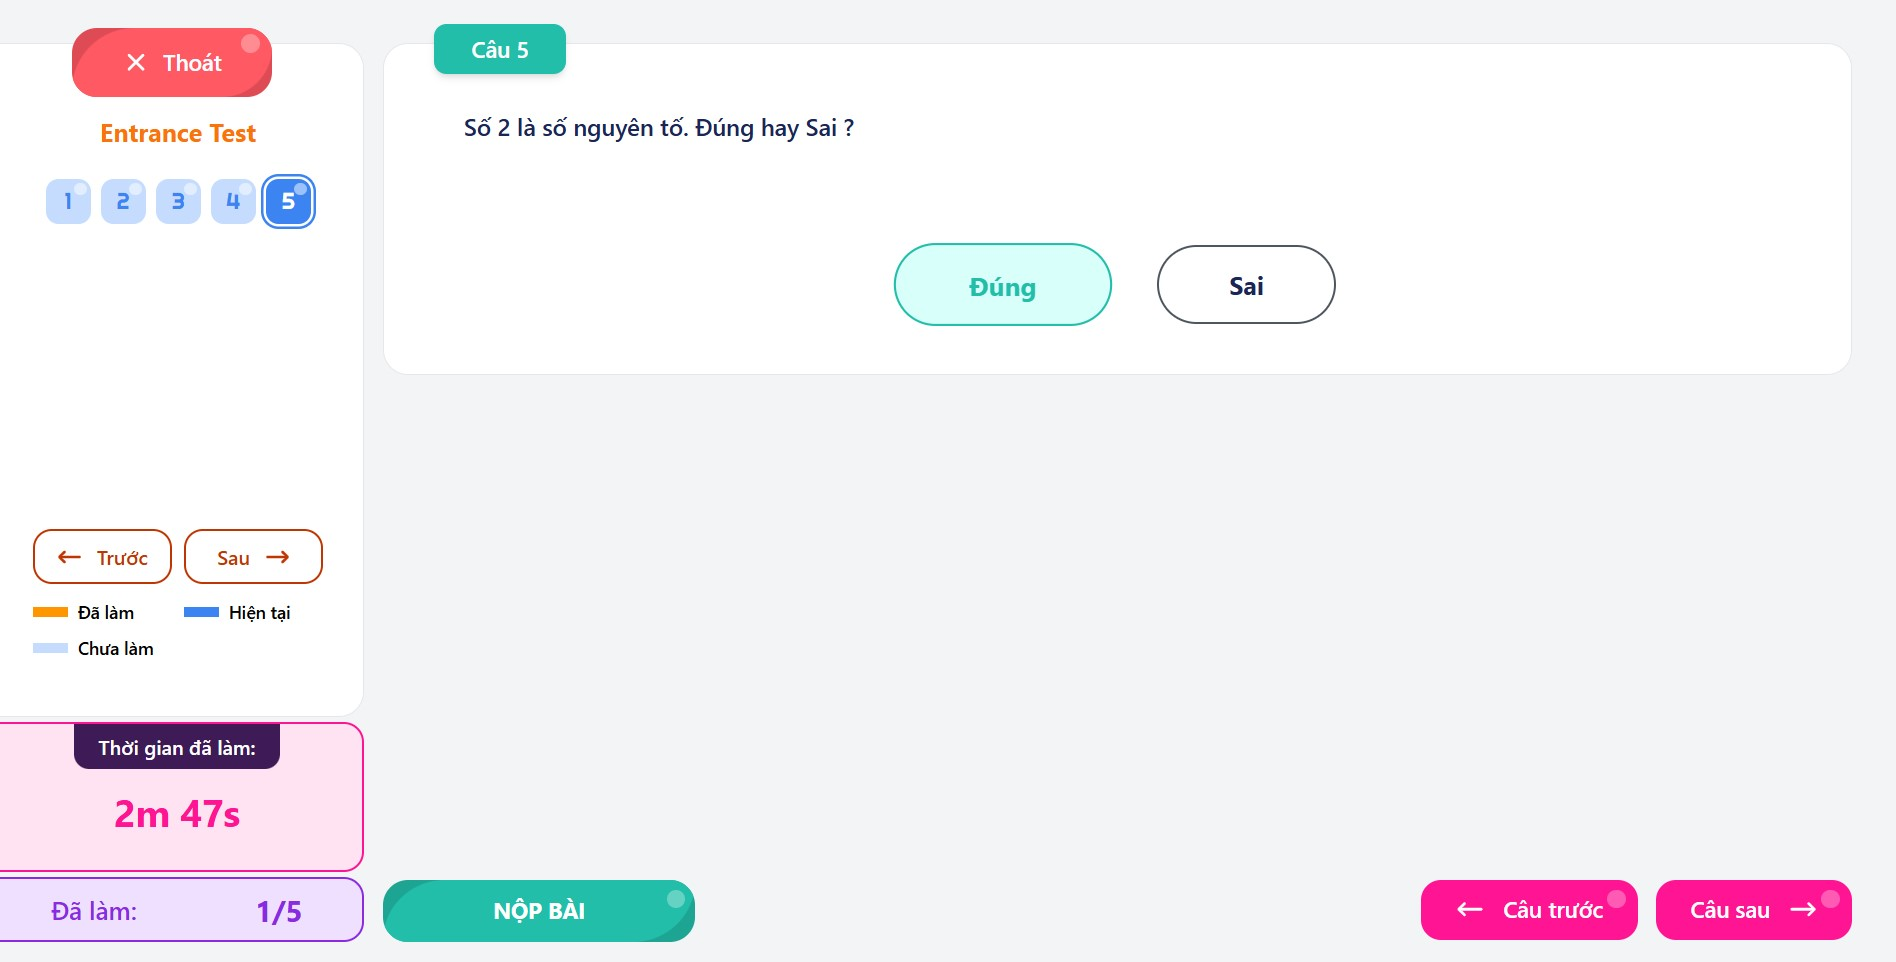
\includegraphics[width=\textwidth]{Image/UI/Main-Student/ExamTF.jpg}
			\vspace{0.2cm}
			\caption{Dạng đúng/sai}
			\label{fig:exam5}
		\end{minipage}
	\end{figure}
	
	\vspace{0.4cm}
\newline
Khi người dùng chưa hoàn thành bài thi nhưng bấm thoát, giao diện sẽ hiển thị một thông báo lưu tiến trình làm bài như \textit{Hình \ref{fig:save}}. Khi người dùng bấm nộp bài, giao diện sẽ hiển thị thông báo để xác nhận như \textit{Hình \ref{fig:submit}}.
	\begin{figure}[H]
		\centering
		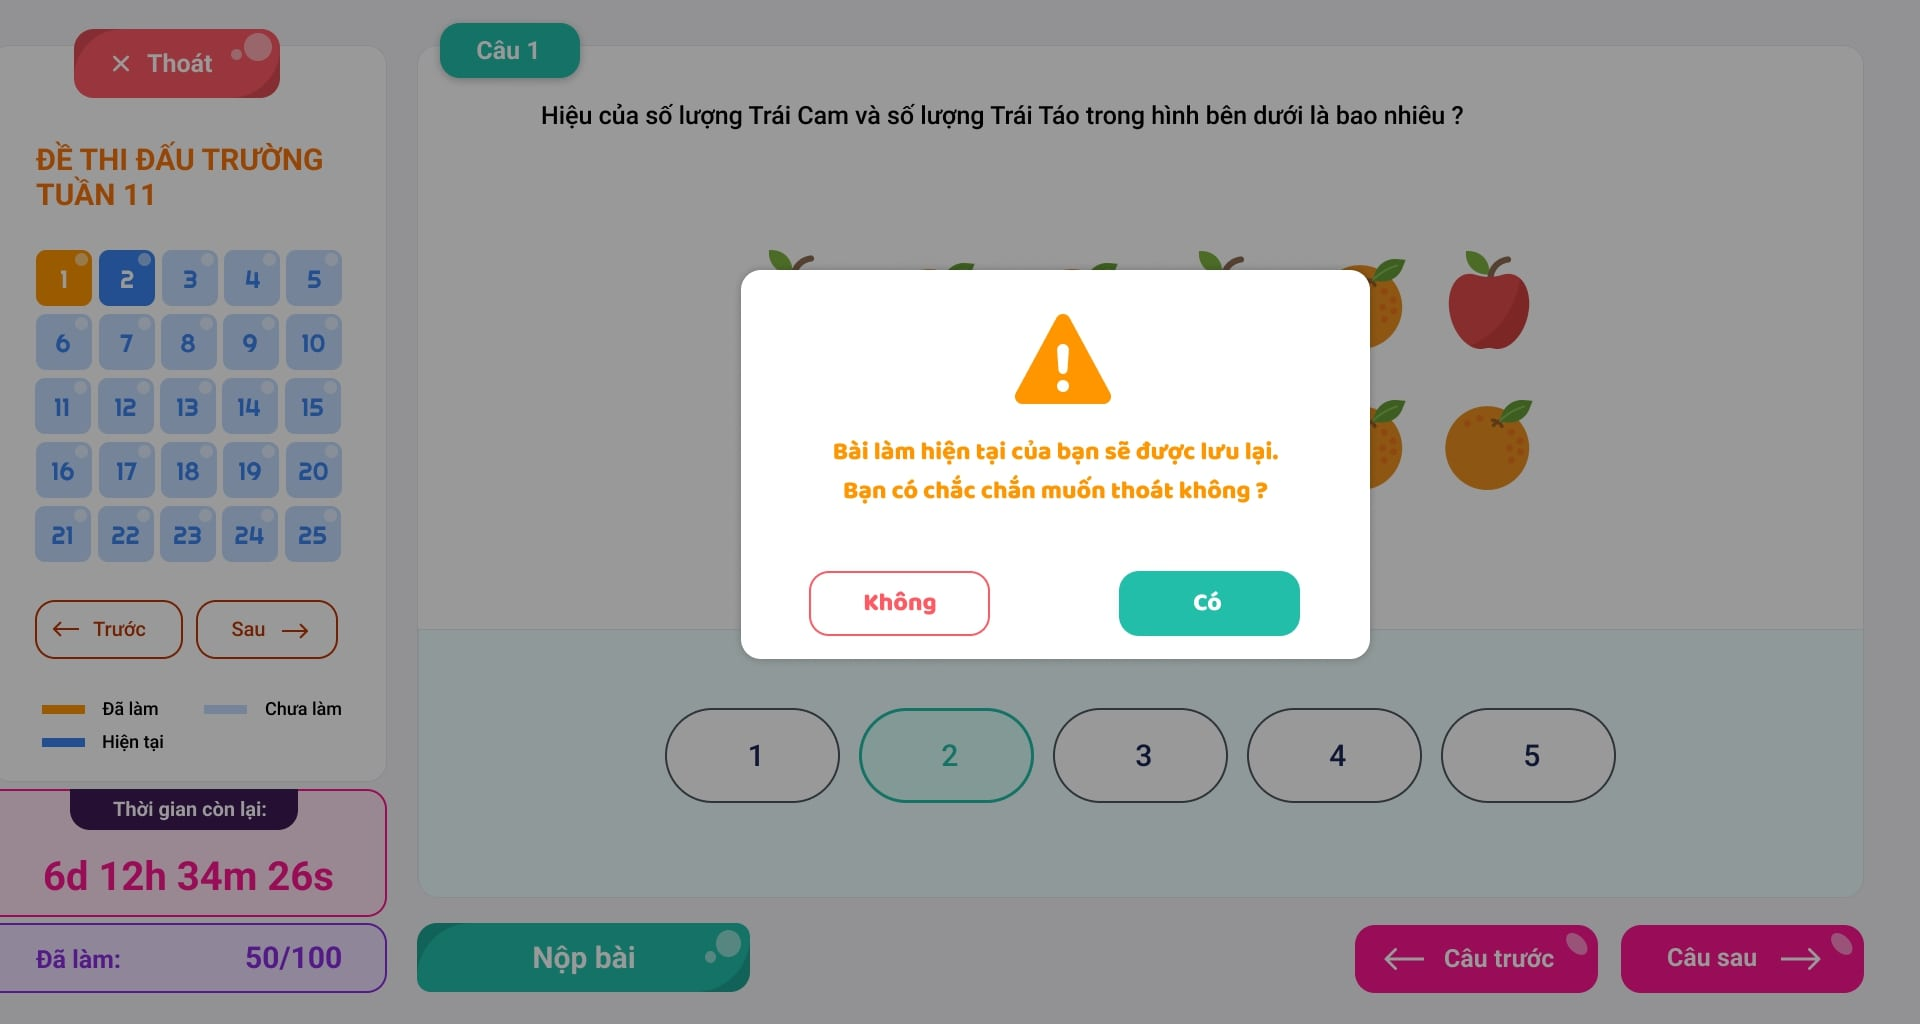
\includegraphics[width=0.9\textwidth]{Image/UI/Main-Student/Exitpopup.jpg}
		\vspace{0.6cm}
		\caption{Trang Bài thi - Thông báo khi thoát}
		\label{fig:save}
	\end{figure}
	\begin{figure}[H]
		\centering
		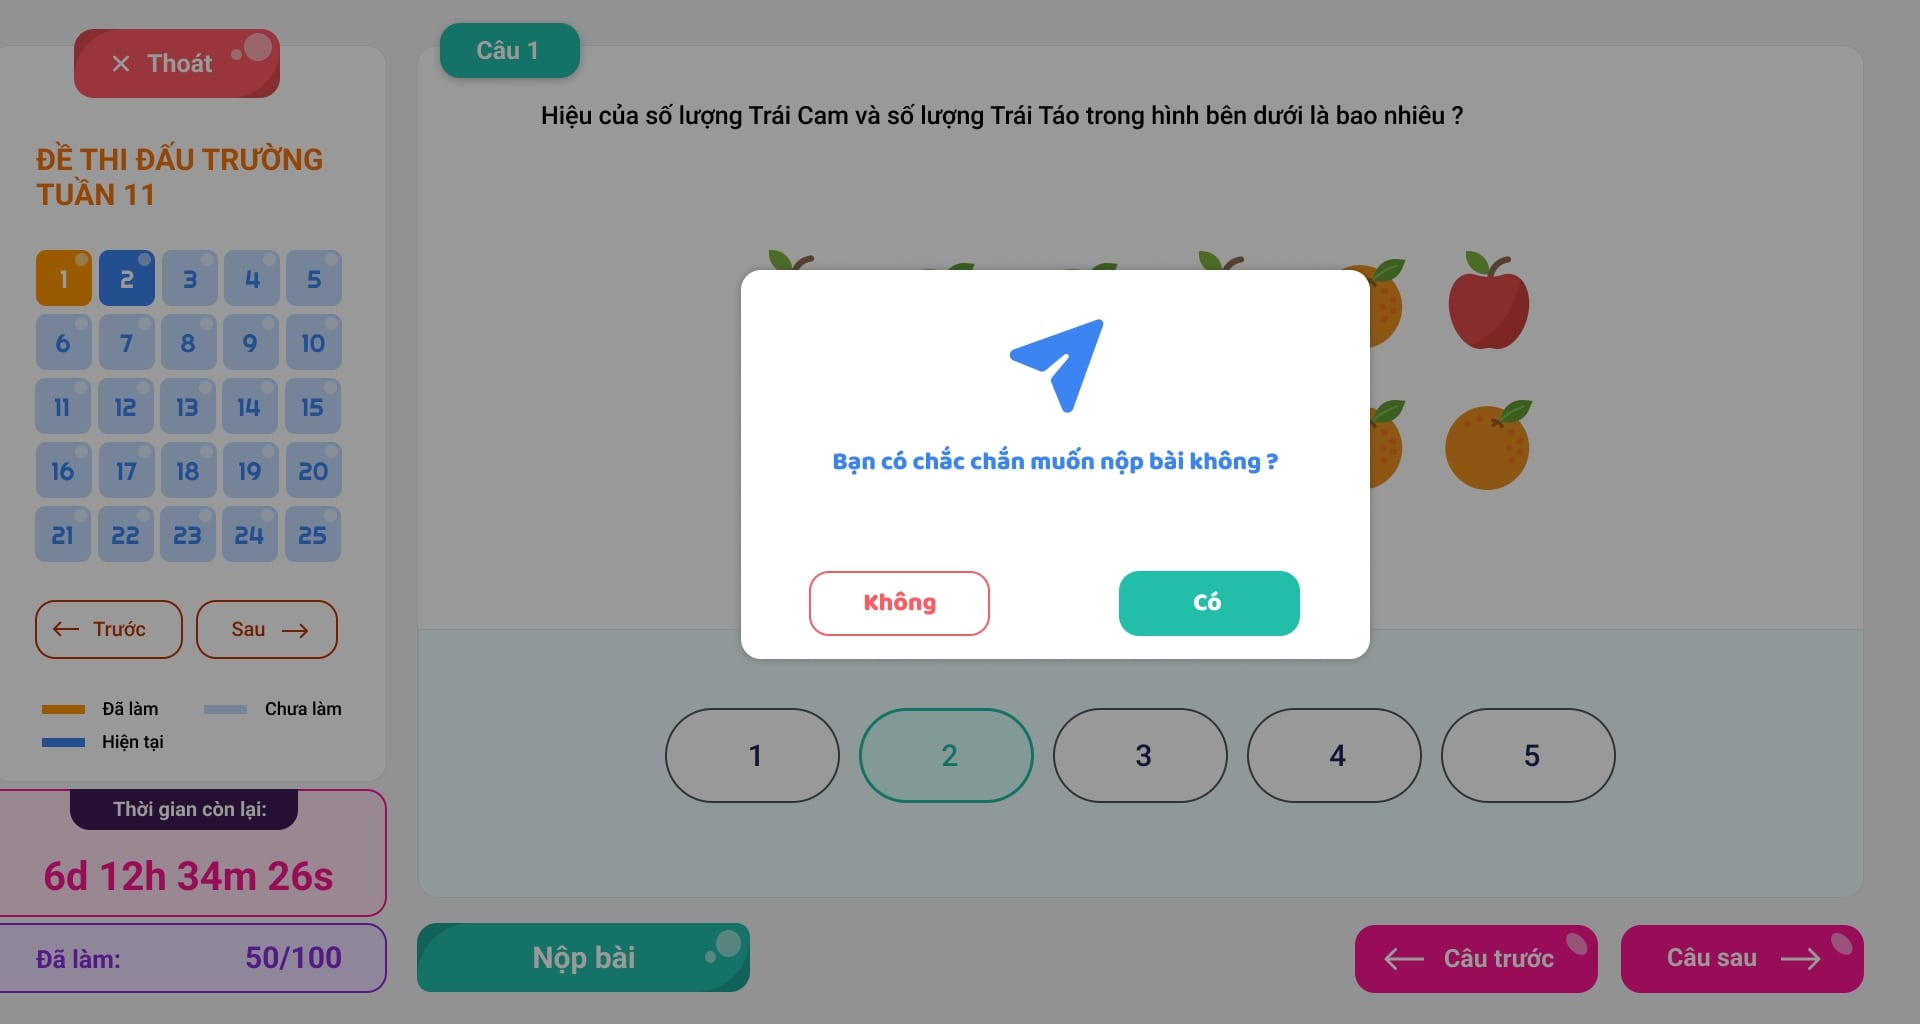
\includegraphics[width=0.9\textwidth]{Image/UI/Main-Student/Submitpopup.jpg}
		\vspace{0.6cm}
		\caption{Trang Bài thi - Thông báo khi bấm nộp bài}
		\label{fig:submit}
	\end{figure}

\subsubsection{Trang Xếp hạng}
Trang xếp hạng sẽ hiển thị top 8 học sinh đạt số lượng thạch anh cao nhất (thạch anh là tiêu chí để xếp hạng học tập), đồng thời vinh danh 3 học sinh xuất sắc nhất. Ngoài ra, trang còn hiển thị số lượng thạch anh mà người dùng đang sở hữu và vị trí xếp hạng hiện tại của người dùng.
	\begin{figure}[H]
		\centering
		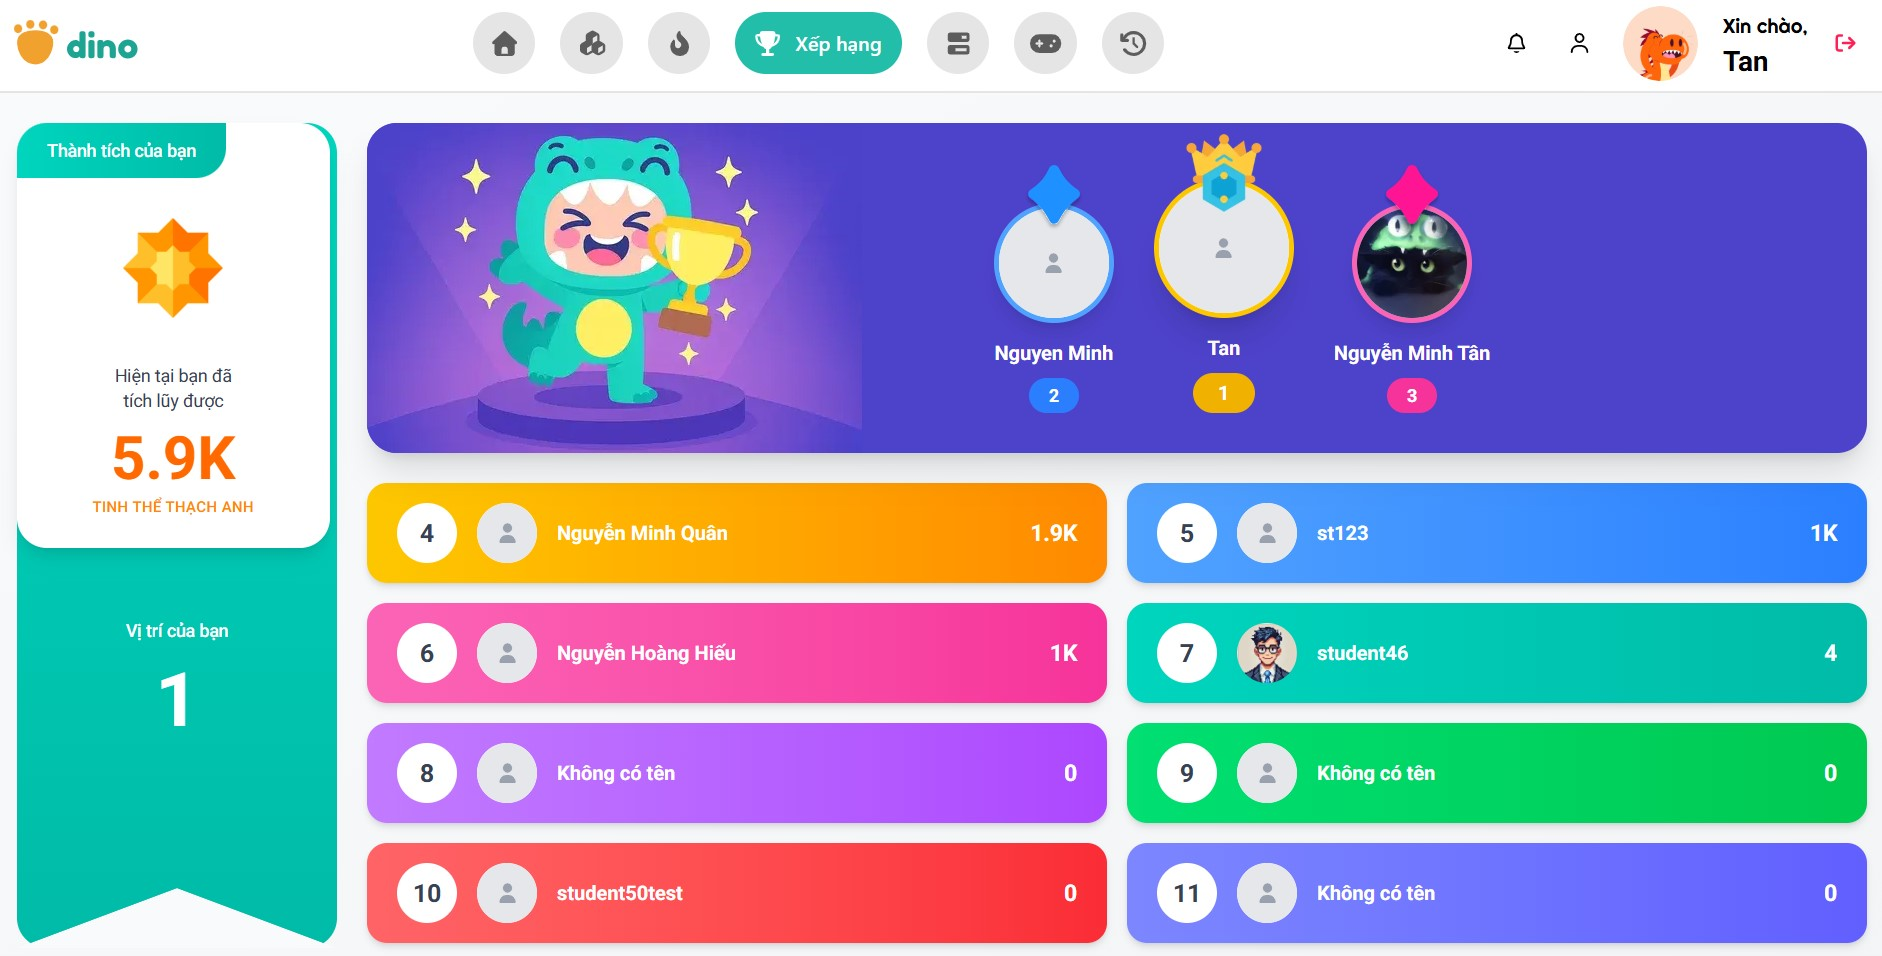
\includegraphics[width=0.9\textwidth]{Image/UI/Main-Student/Leaderboard2.jpg}
		\vspace{0.6cm}
		\caption{Trang Xếp hạng}
	\end{figure}

\subsubsection{Trang Nhiệm vụ}
Trang nhiệm vụ hiển thị các nhiệm vụ hệ thống, phần thưởng là thạch anh. Nếu người dùng hoàn thành được nhiệm vụ đó thì họ có thể nhận phần thưởng tương ứng. Người dùng còn có thể xem các nhiệm vụ đã hoàn thành và các nhiệm vụ chưa hoàn thành.
\begin{figure}[H]
	\centering
	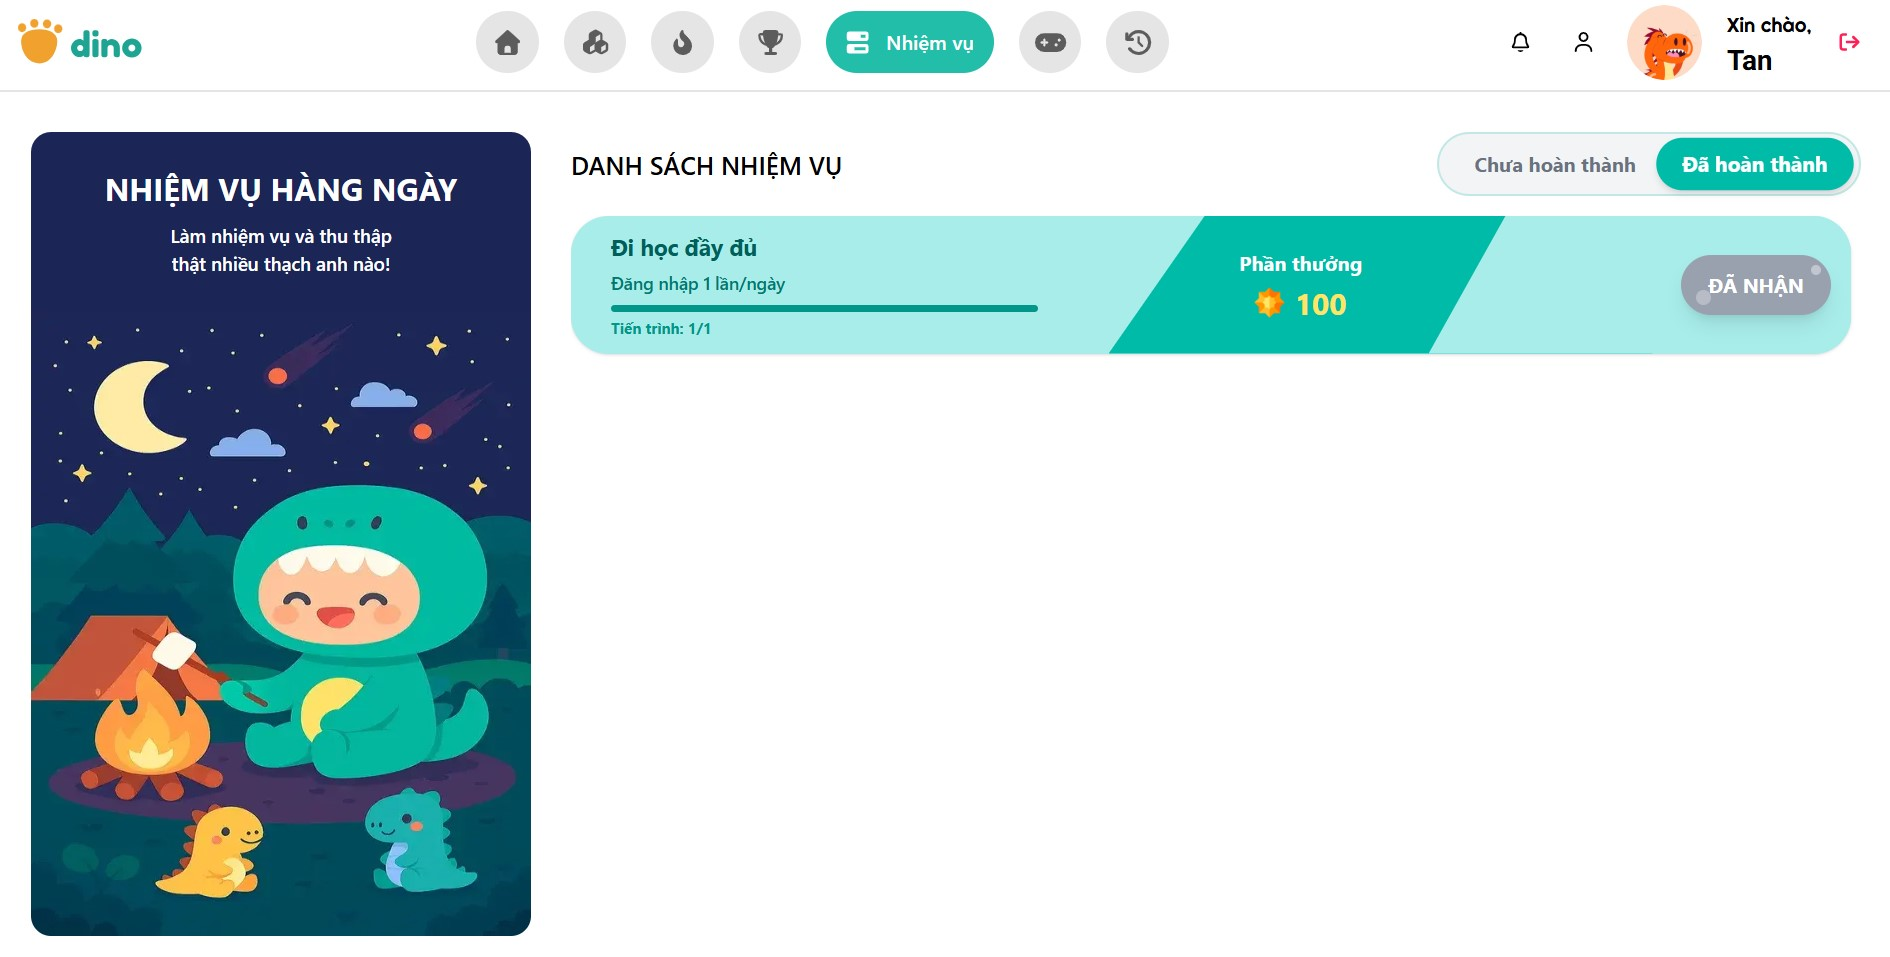
\includegraphics[width=0.9\textwidth]{Image/UI/Main-Student/MissionComplete.jpg}
	\vspace{0.6cm}
	\caption{Trang Nhiệm vụ - Đã hoàn thành}
\end{figure}
\begin{figure}[H]
	\centering
	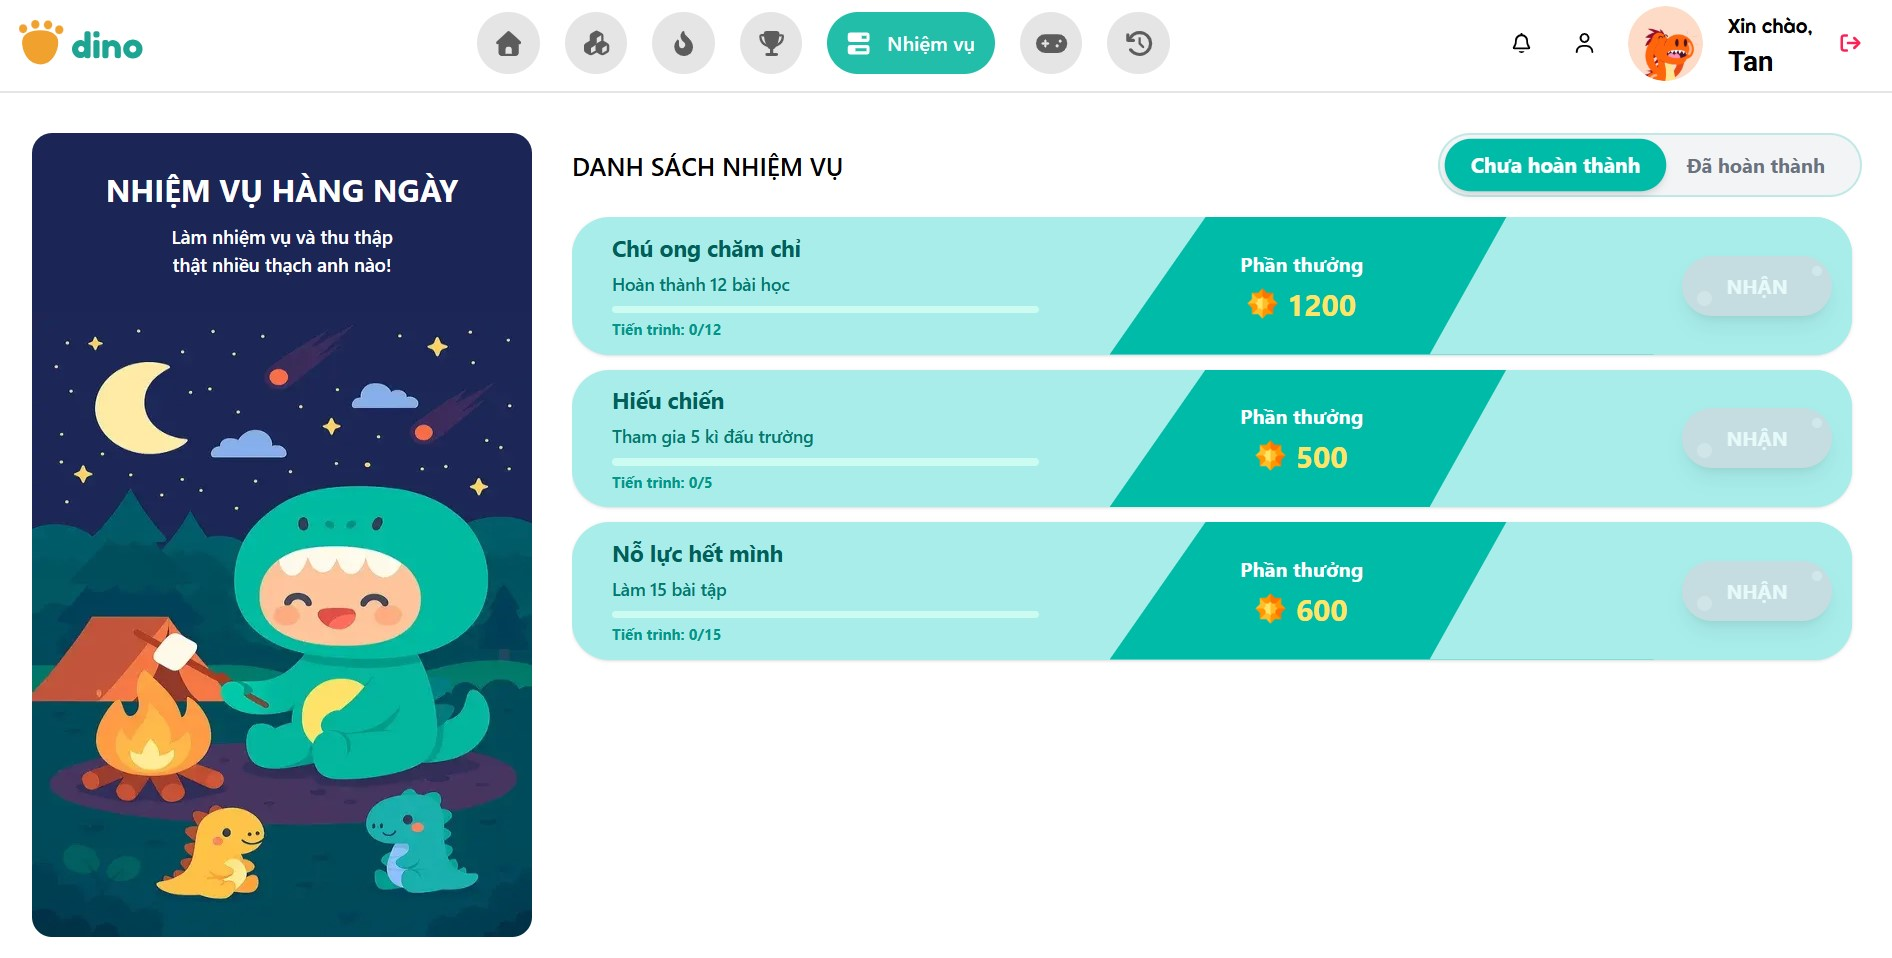
\includegraphics[width=0.9\textwidth]{Image/UI/Main-Student/MissionIncomplete.jpg}
	\vspace{0.6cm}
	\caption{Trang Nhiệm vụ - Chưa hoàn thành}
\end{figure}
\begin{figure}[H]
	\centering
	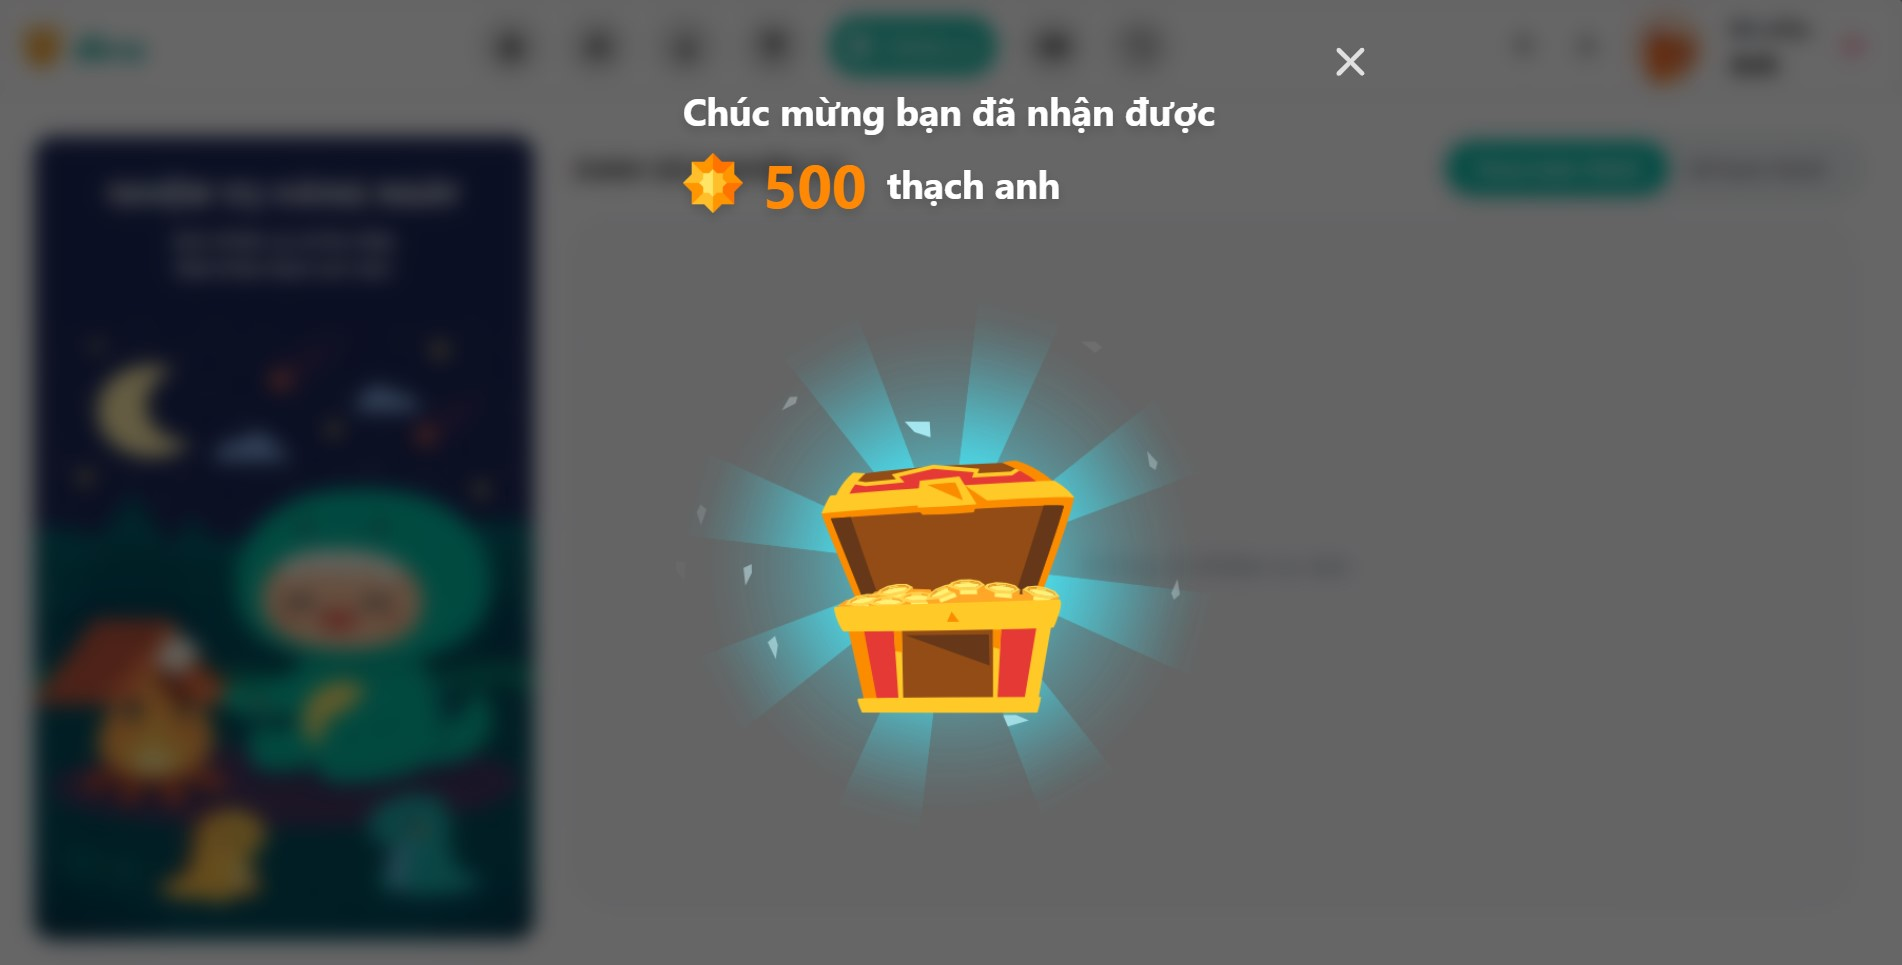
\includegraphics[width=0.9\textwidth]{Image/UI/Main-Student/ClaimMission.jpg}
	\vspace{0.6cm}
	\caption{Trang Nhiệm vụ - Nhận thưởng}
\end{figure}

\newpage
\subsubsection{Trang Minigames}
\label{subsubsec:games}
Trang Minigames hiển thị các Minigame bao gồm hai loại chính: Game chơi đơn - nơi người dùng giải quyết các trò chơi toán học cá nhân; và Game tương tác cho phép học sinh đối đầu hoặc hợp tác với phụ huynh và các thành viên khác trong Family để cùng giải toán. Tại đây, người dùng có thể tham gia trò chơi ngay lập tức bằng cách bấm vào nút \textit{Chơi ngay}, sau đó, một tab mới trên trình duyệt sẽ được mở và giao diện trò chơi được hiển thị, ví dụ như \textit{Hình \ref{fig:mathmatch}}.
\begin{figure}[H]
	\centering
	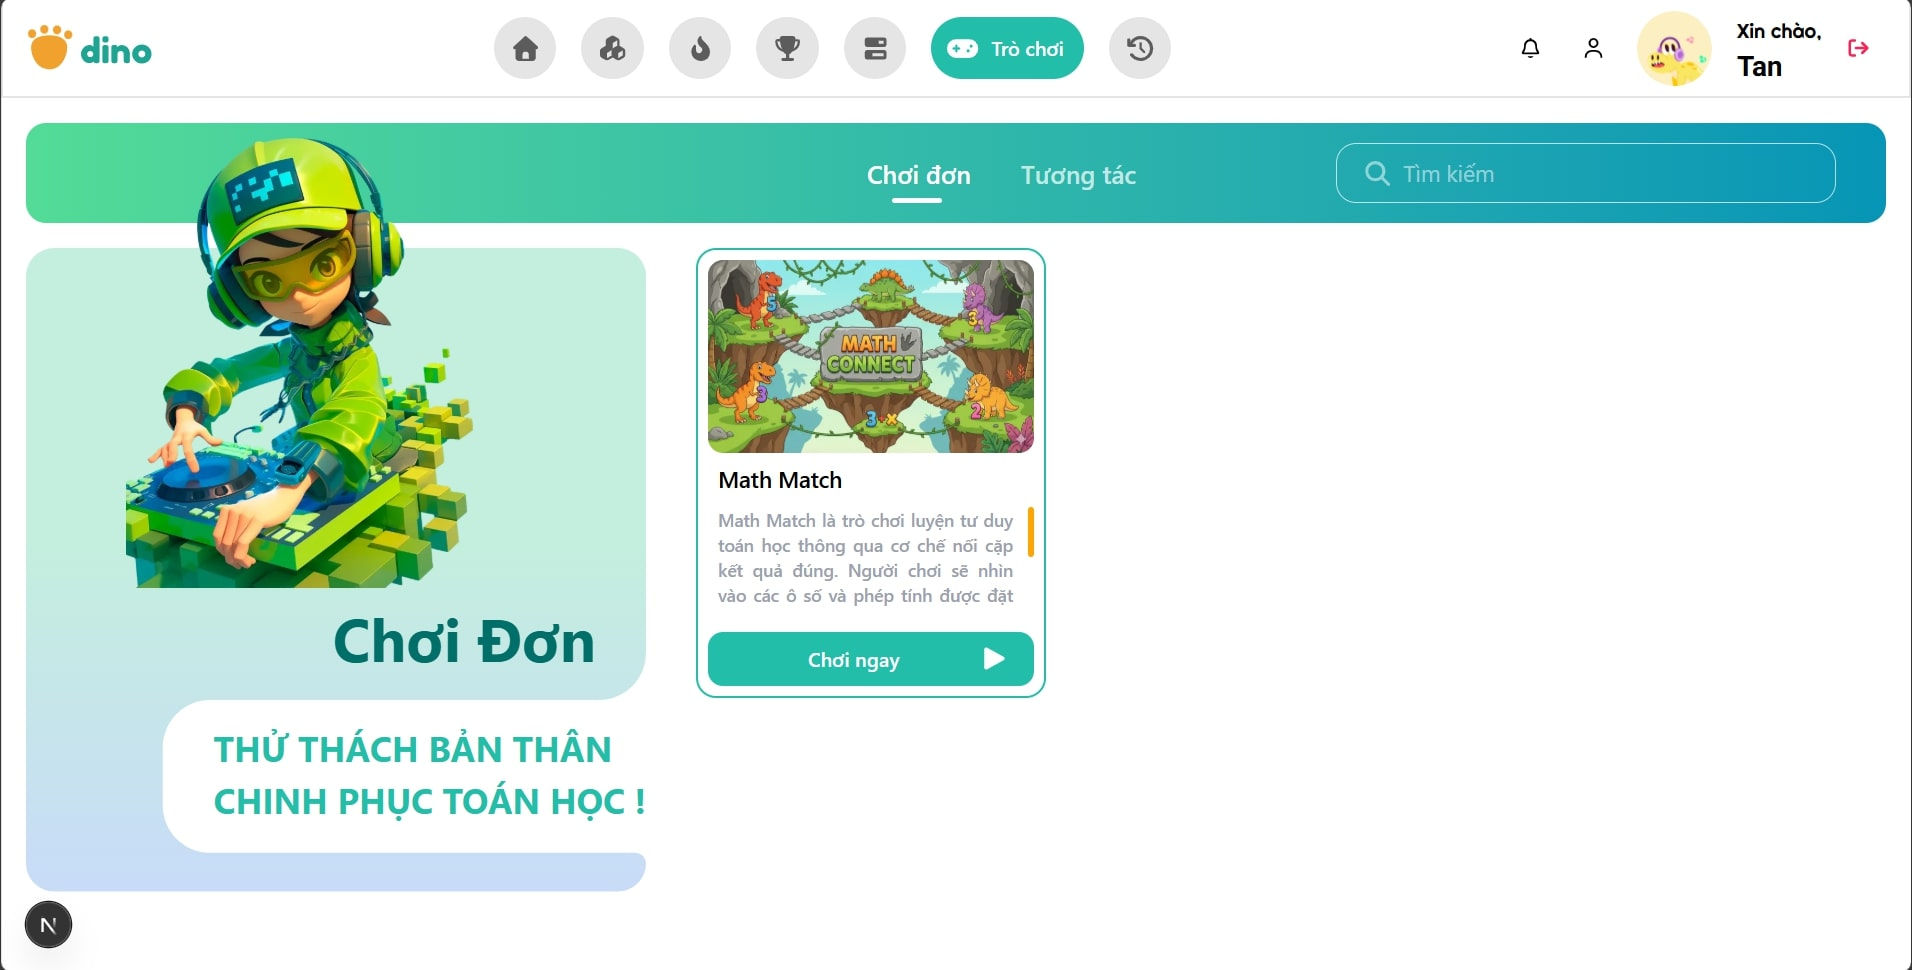
\includegraphics[width=0.9\textwidth]{Image/UI/Main-Student/Game-Single.jpg}
	\vspace{0.6cm}
	\caption{Trang Minigame - Chơi đơn}
\end{figure}
\begin{figure}[H]
	\centering
	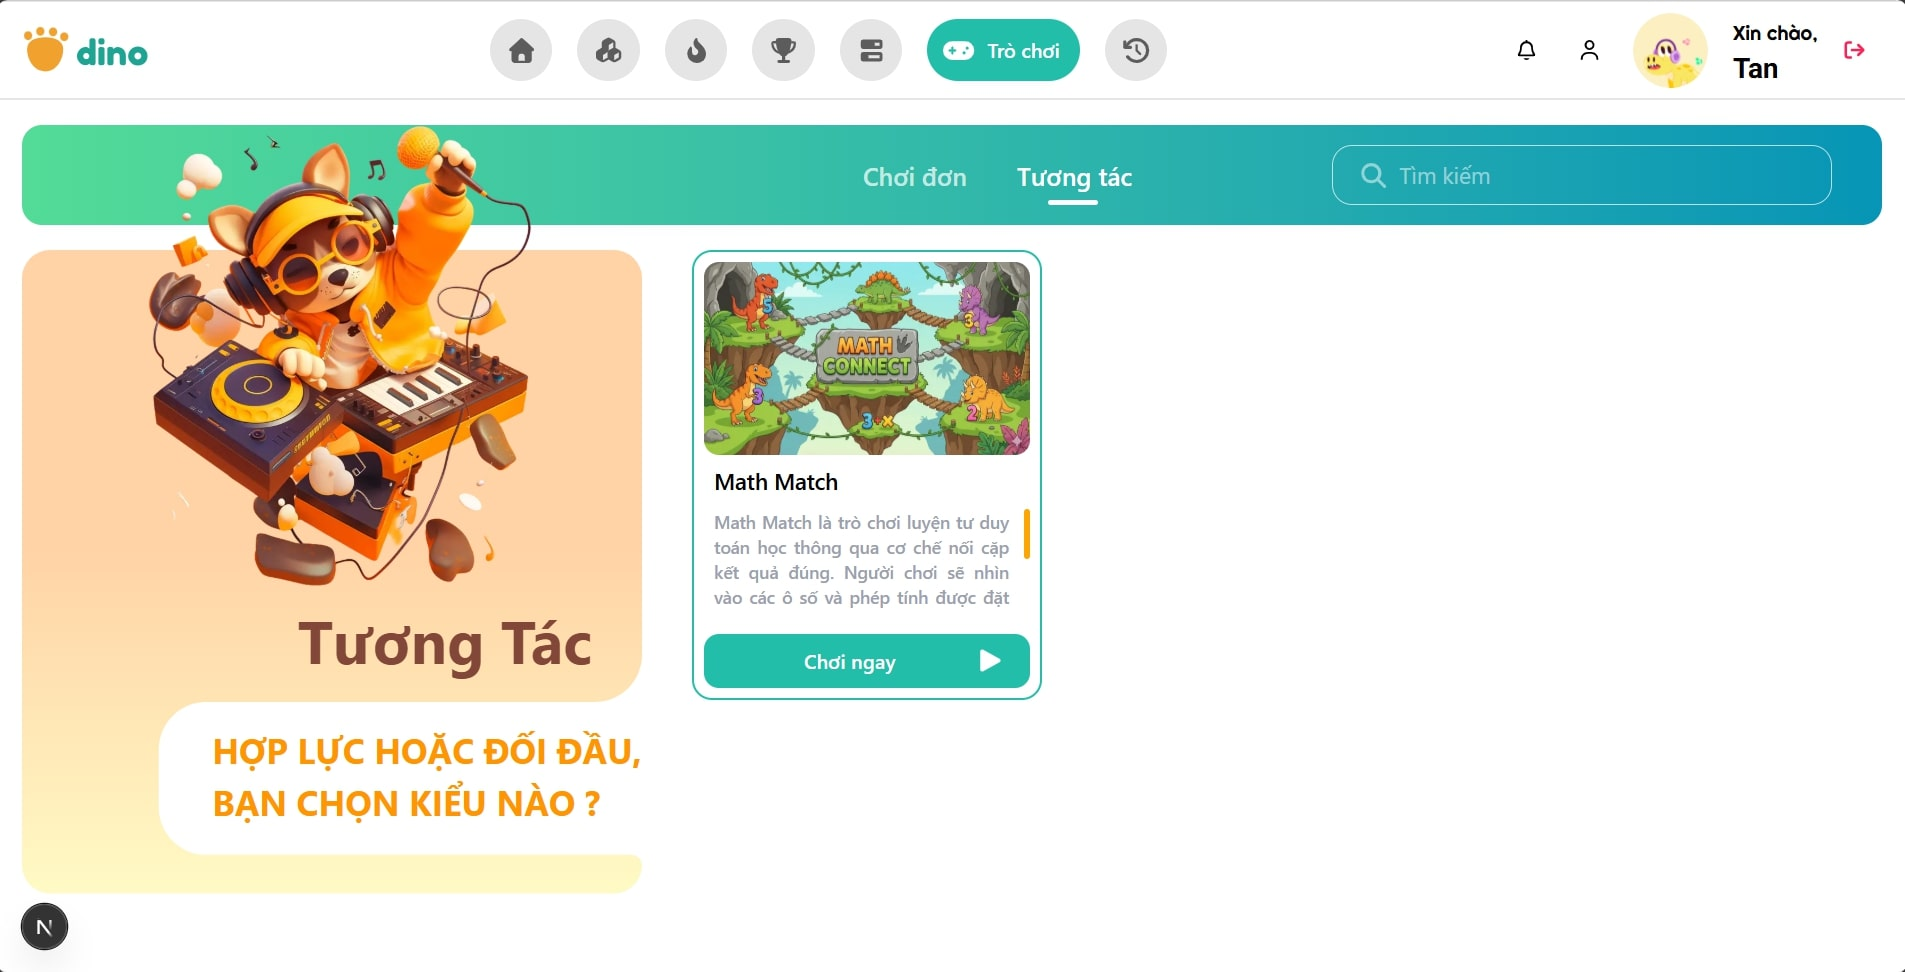
\includegraphics[width=0.9\textwidth]{Image/UI/Main-Student/Game-PVP.jpg}
	\vspace{0.6cm}
	\caption{Trang Minigame - Tương tác}
\end{figure}

\newpage
Minigame chơi đơn có tên gọi \textbf{Math Match}. Đây là trò chơi mang lối chơi tương tự như game Pikachu cổ điển, nơi người chơi cần tìm và nối các cặp ô phù hợp để loại bỏ chúng khỏi màn hình. Tuy nhiên, thay vì nối các hình giống nhau, người chơi trong Math Match phải nối các phép tính có \textbf{kết quả bằng nhau}. Điều này không chỉ tạo sự quen thuộc về cơ chế chơi mà còn tăng thêm yếu tố tư duy và tính toán.

Trong quá trình chơi, người chơi cần quan sát nhanh, tính toán chính xác và lựa chọn đường nối hợp lệ giữa các ô để hoàn thành màn chơi trong thời gian giới hạn. Để tăng tính hấp dẫn và hỗ trợ người chơi trong những tình huống khó, game còn được tích hợp thêm các \textbf{item bổ trợ}. Ví dụ, item dạng “rocket” có thể giúp phá hủy một số ô bất kỳ trên màn hình, tạo ra khoảng trống thuận lợi cho việc nối các cặp còn lại. Bên cạnh đó, item “hint” sẽ gợi ý các cặp ô có thể nối được, giúp người chơi tiếp tục khi không tìm thấy nước đi

Sự kết hợp giữa yếu tố giải đố, tính toán và các cơ chế hỗ trợ đã giúp Math Match trở nên thú vị hơn, vừa mang tính giải trí vừa góp phần rèn luyện khả năng tư duy logic và phản xạ của người chơi.
\begin{figure}[H]
	\centering
	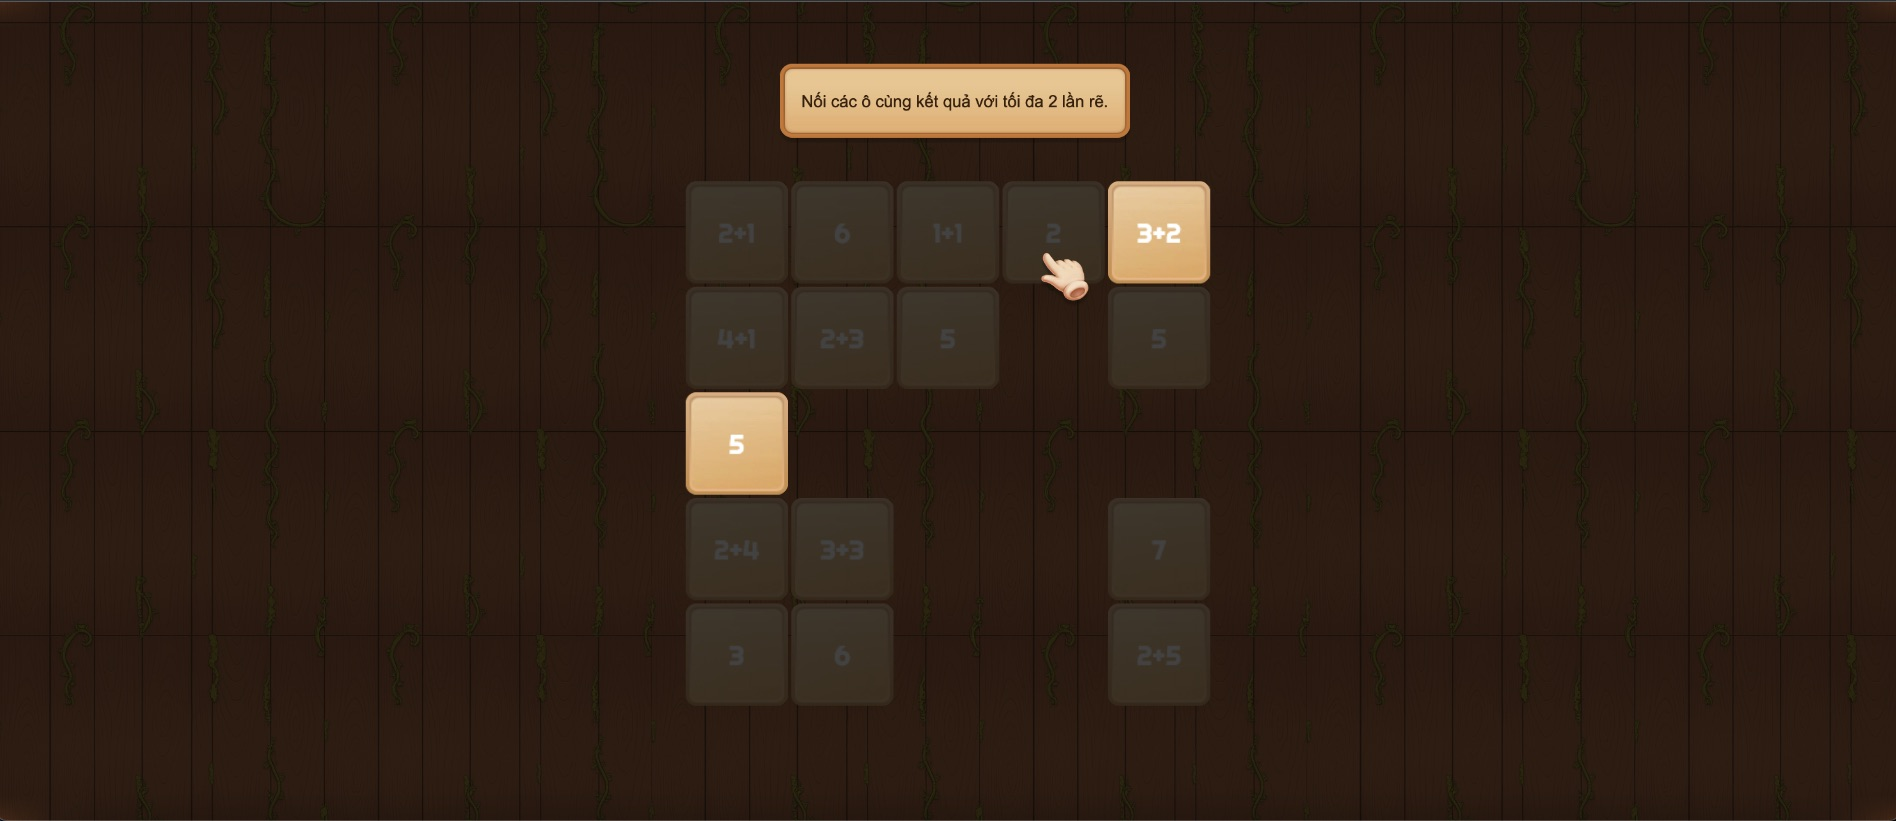
\includegraphics[width=0.9\textwidth]{Image/UI/Main-Student/MathMatchGame.jpeg}
	\vspace{0.6cm}
	\caption{Trang Minigame - Minigame Math Match}
	\label{fig:mathmatch}
\end{figure}

\newpage
 Minigame tương tác 2 người với tên gọi \textbf{Tomato Shooting}. Game được lấy ý tưởng từ tựa game Gunny, trong đó hai người chơi đối đầu trực tiếp với nhau theo thời gian thực thông qua máy chủ đa người chơi \textbf{Colyseus} tích hợp trong Cocos Creator. Mỗi màn chơi bao gồm 5 vòng, mỗi vòng hệ thống sẽ hiển thị một phép tính toán học, người chơi phải bắn quả cà chua tới quả bóng mang kết quả đúng trước đối thủ để giành chiến thắng trong vòng đó. Sau 5 vòng, người chơi nào thắng nhiều vòng hơn sẽ là người chiến thắng chung cuộc. Cơ chế thời gian thực và yếu tố cạnh tranh trực tiếp giúp tăng tính hấp dẫn, đồng thời vẫn đảm bảo mục tiêu luyện tập tính toán nhanh cho học sinh.
\begin{figure}[H]
	\centering
	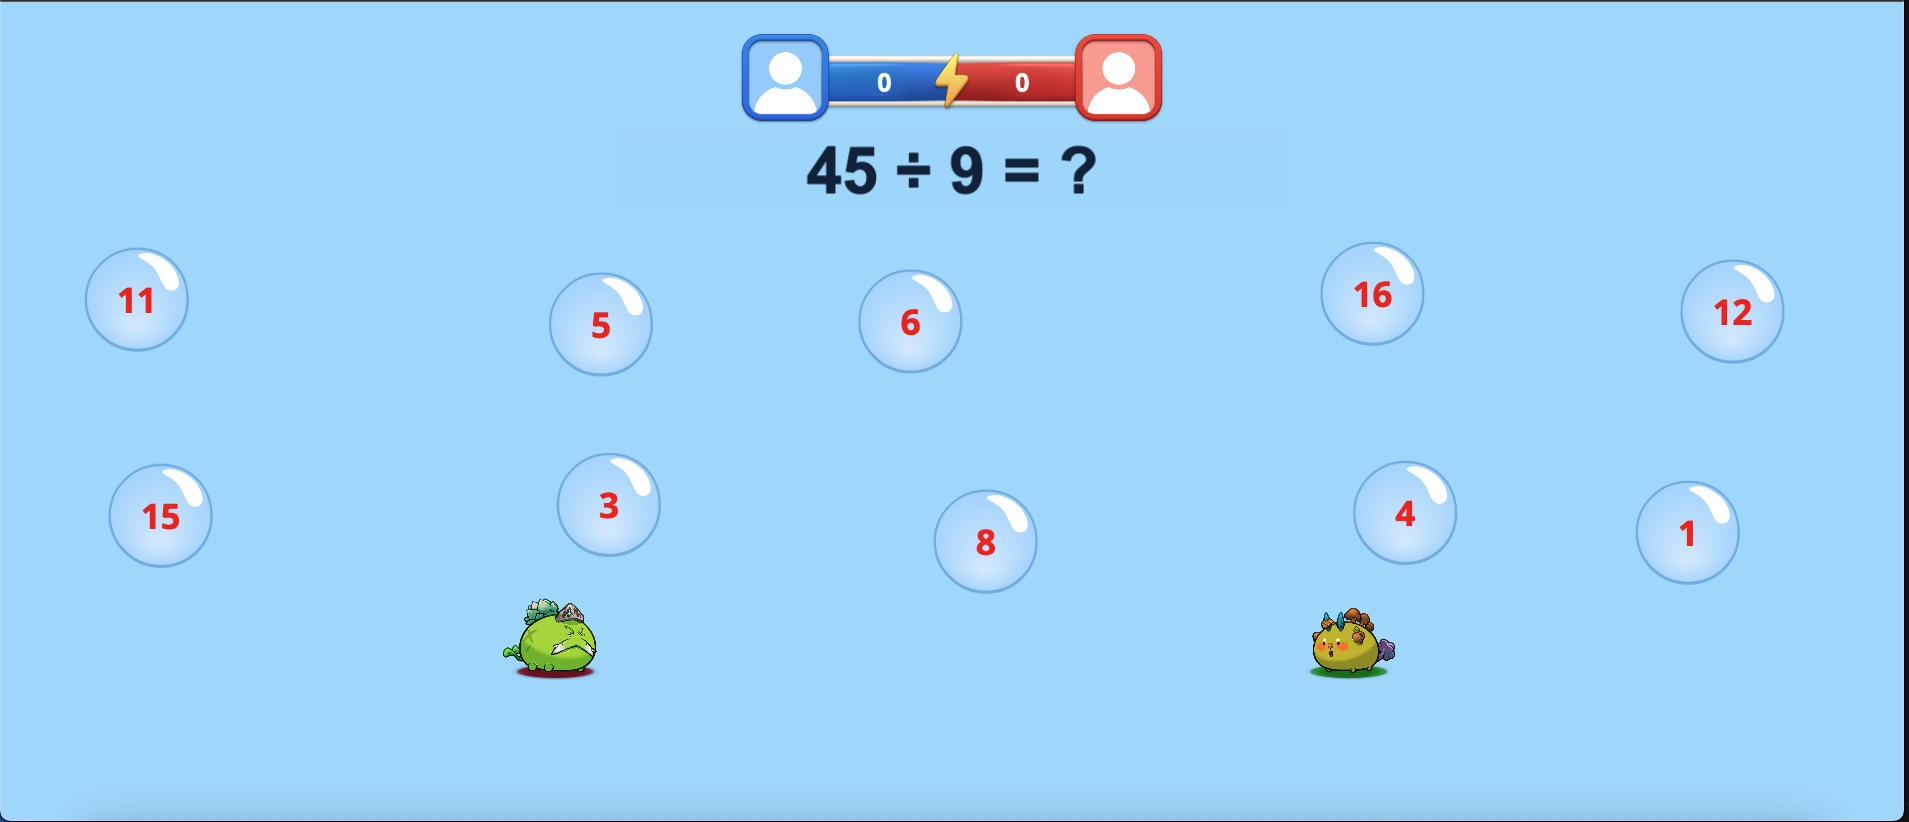
\includegraphics[width=0.9\textwidth]{Image/UI/Main-Student/TomatoesShootingGame.jpeg}
	\vspace{0.6cm}
	\caption{Trang Minigame - Minigame Tomato Shooting}
	\label{fig:tomatoshooting}
\end{figure}

\subsubsection{Trang Lịch sử làm bài}
Người dùng có thể dễ dàng theo dõi tiến độ thông qua việc lọc lịch sử làm bài và xem các chỉ số thống kê về số lượng, độ chính xác trung bình của bài tập. Giao diện chính của trang lịch sử làm bài được thiết kế như hình bên dưới.
\begin{figure}[H]
	\centering
	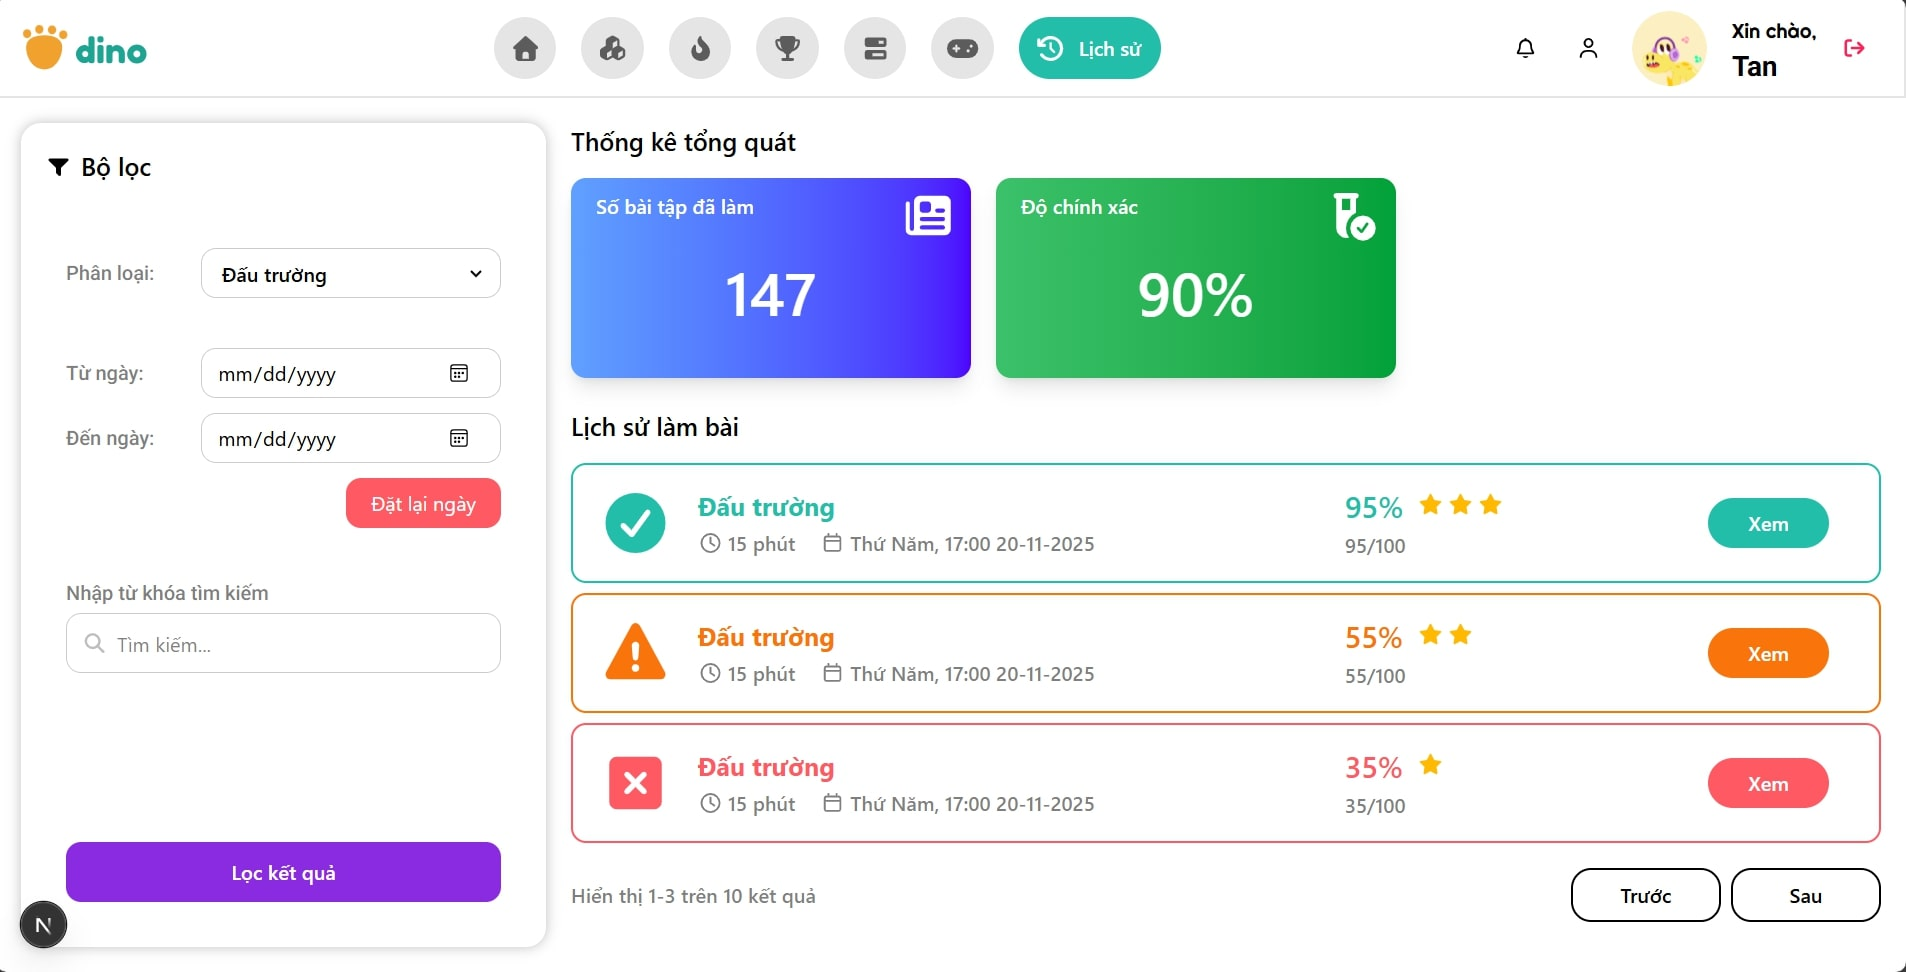
\includegraphics[width=0.9\textwidth]{Image/UI/Main-Student/History.jpg}
	\vspace{0.6cm}
	\caption{Trang Lịch sử làm bài}
	\label{fig:history}
\end{figure}

\newpage
Khi bấm vào nút \textit{Xem} trên các bản ghi được hiển thị ở  \textit{Hình \ref{fig:history}}, người dùng còn có thể xem chi tiết bài làm với các thông tin như: thời gian làm bài, thời gian hoàn thành, tổng số câu, số câu đúng, số câu sai. Đặc biệt, người dùng có thể biết mình làm sai hoặc đúng câu nào cũng như đáp án chính xác của câu đó. Giao diện chi tiết bài làm được thiết kế như 2 hình dưới đây.
\begin{figure}[H]
	\centering
	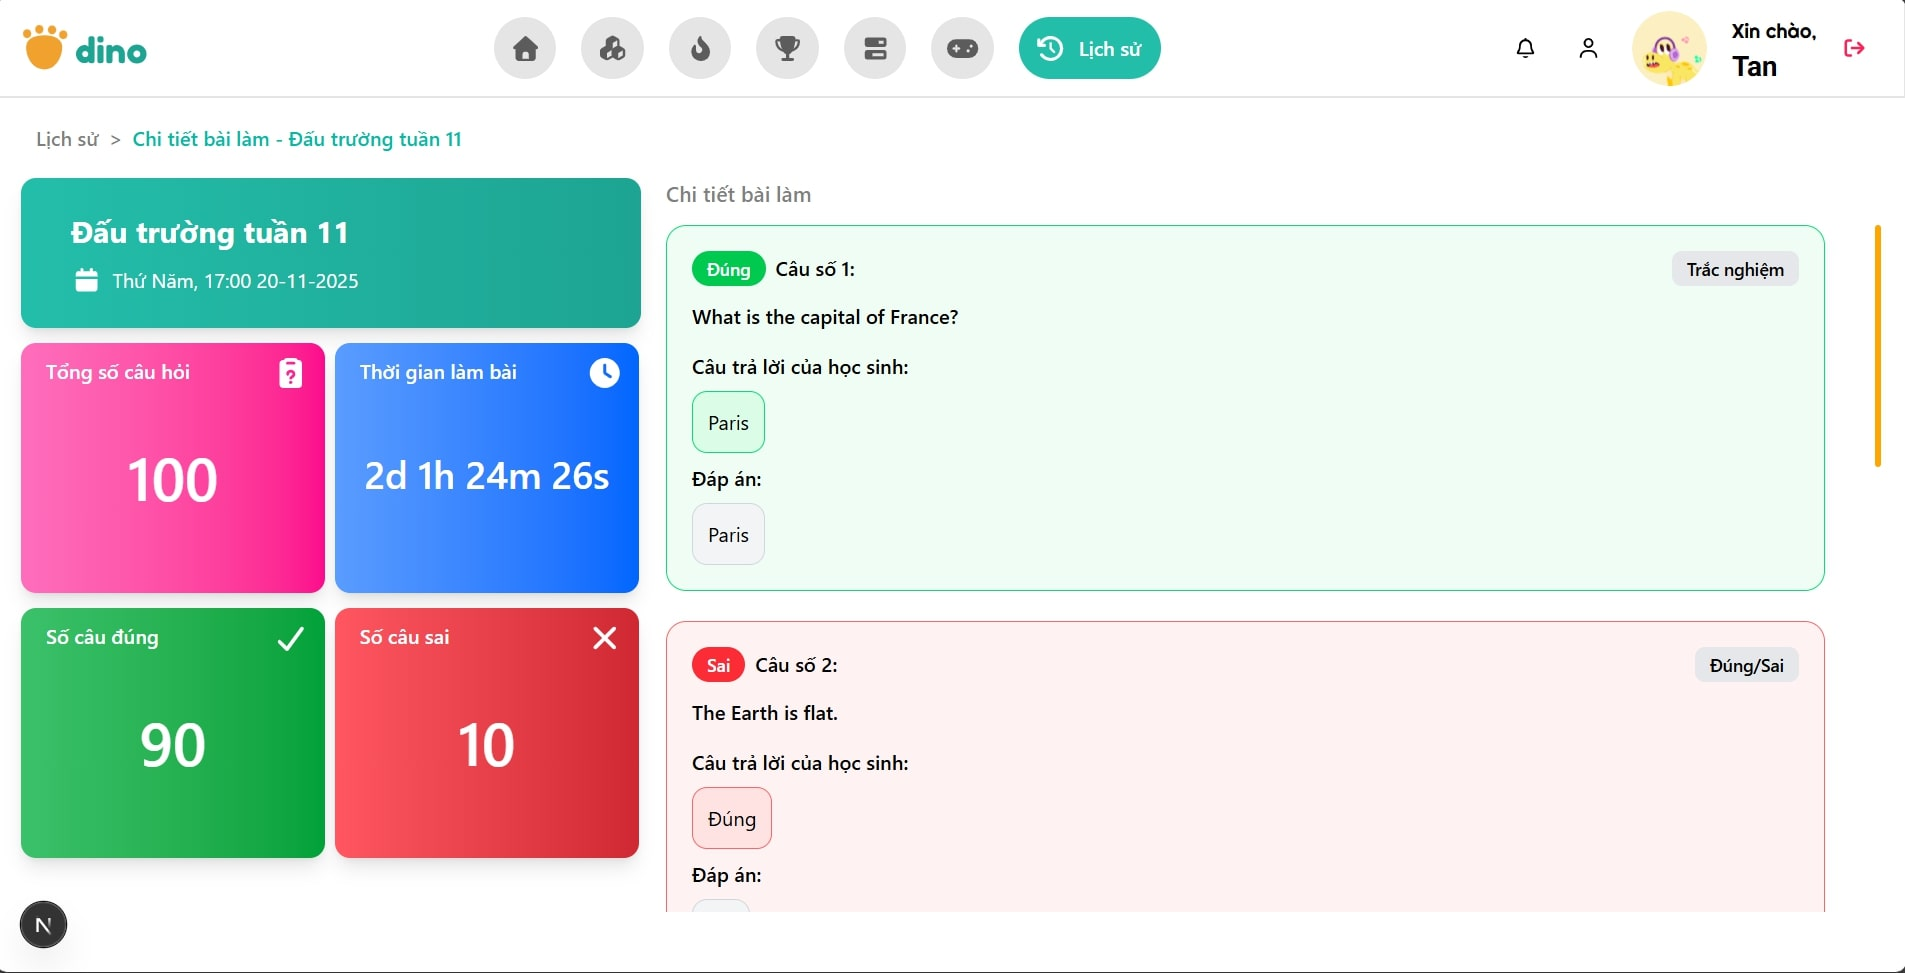
\includegraphics[width=0.9\textwidth]{Image/UI/Main-Student/ExamDetail1.jpg}
	\vspace{0.6cm}
	\caption{Trang Lịch sử làm bài - Chi tiết bài làm}
\end{figure}
\begin{figure}[H]
	\centering
	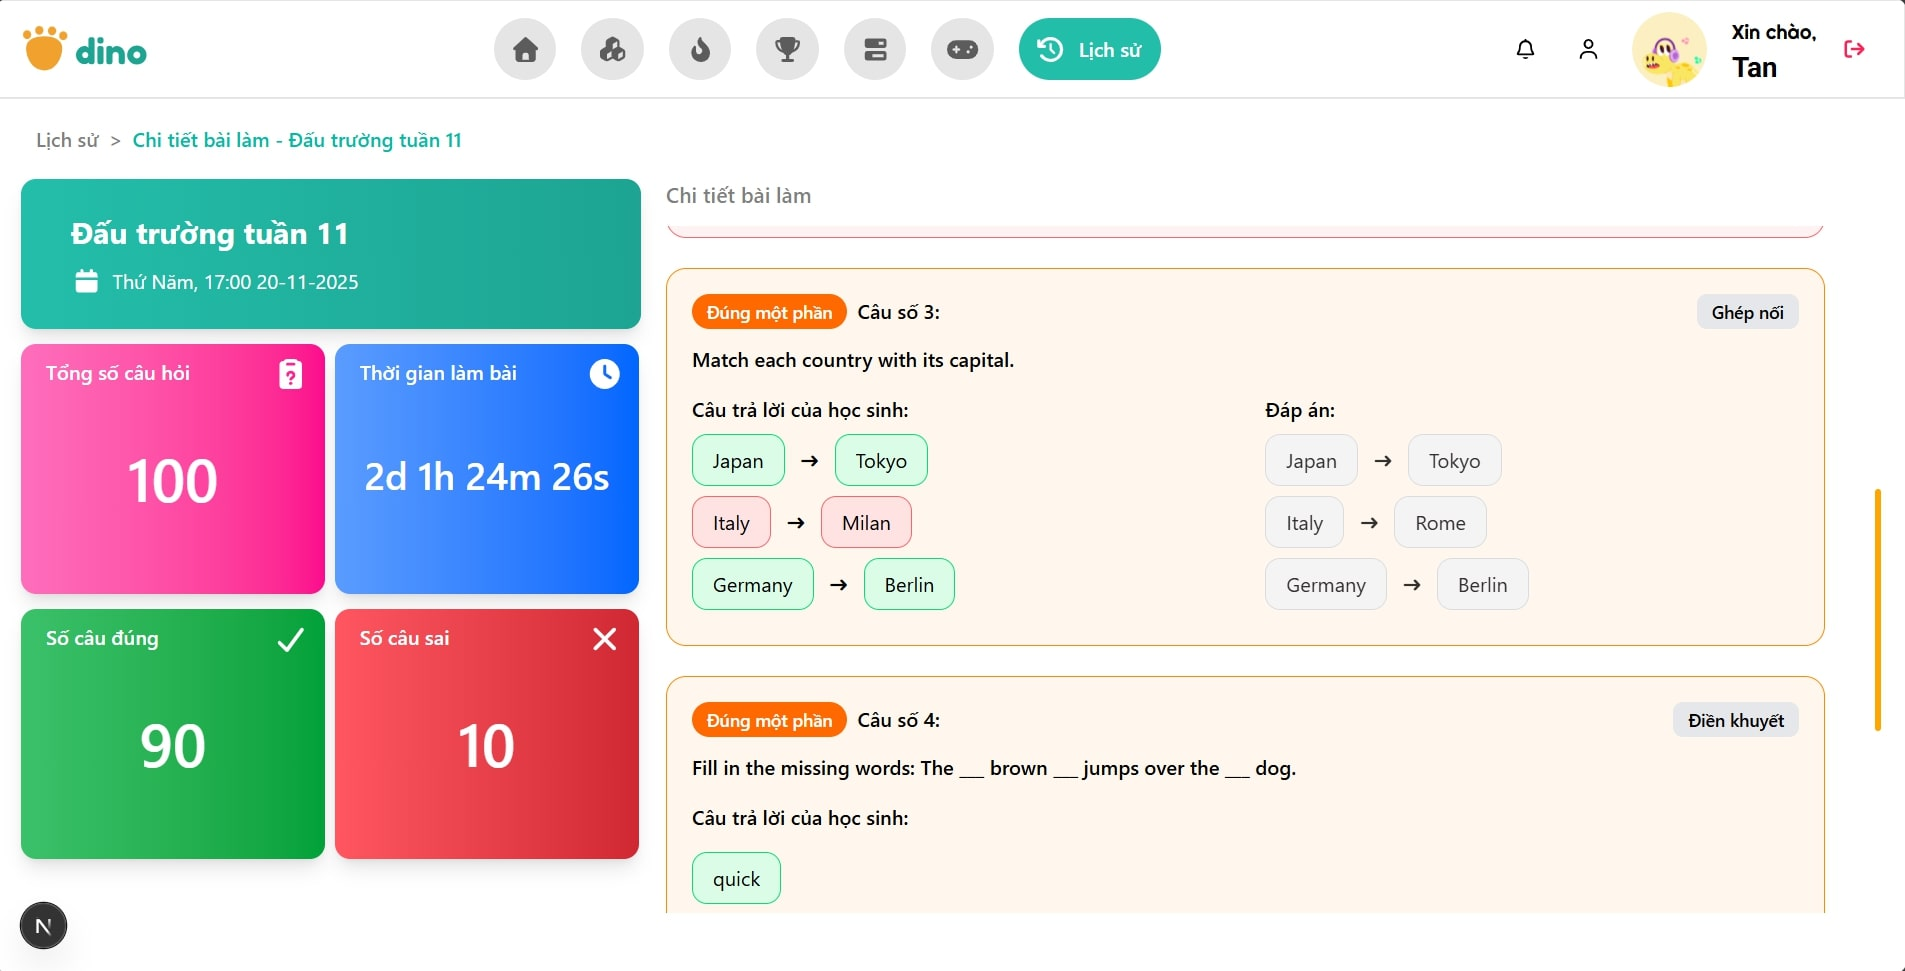
\includegraphics[width=0.9\textwidth]{Image/UI/Main-Student/ExamDetail2.jpg}
	\vspace{0.6cm}
	\caption{Trang Lịch sử làm bài - Chi tiết bài làm}
\end{figure}

\newpage
\subsubsection{Quản lý tài khoản cá nhân}
\label{subsubsec:profile}
\begin{enumerate}
\item \textbf{Xem và cập nhật thông tin cá nhân}
\vspace{0.1cm}
\newline
	Học sinh có thể xem và chỉnh sửa thông tin cá nhân, bao gồm ảnh đại diện, họ và tên, khối lớp. Tuy nhiên, email là cố định với mỗi tài khoản và chỉ được quyền xem.
	\begin{figure}[H]
		\centering
		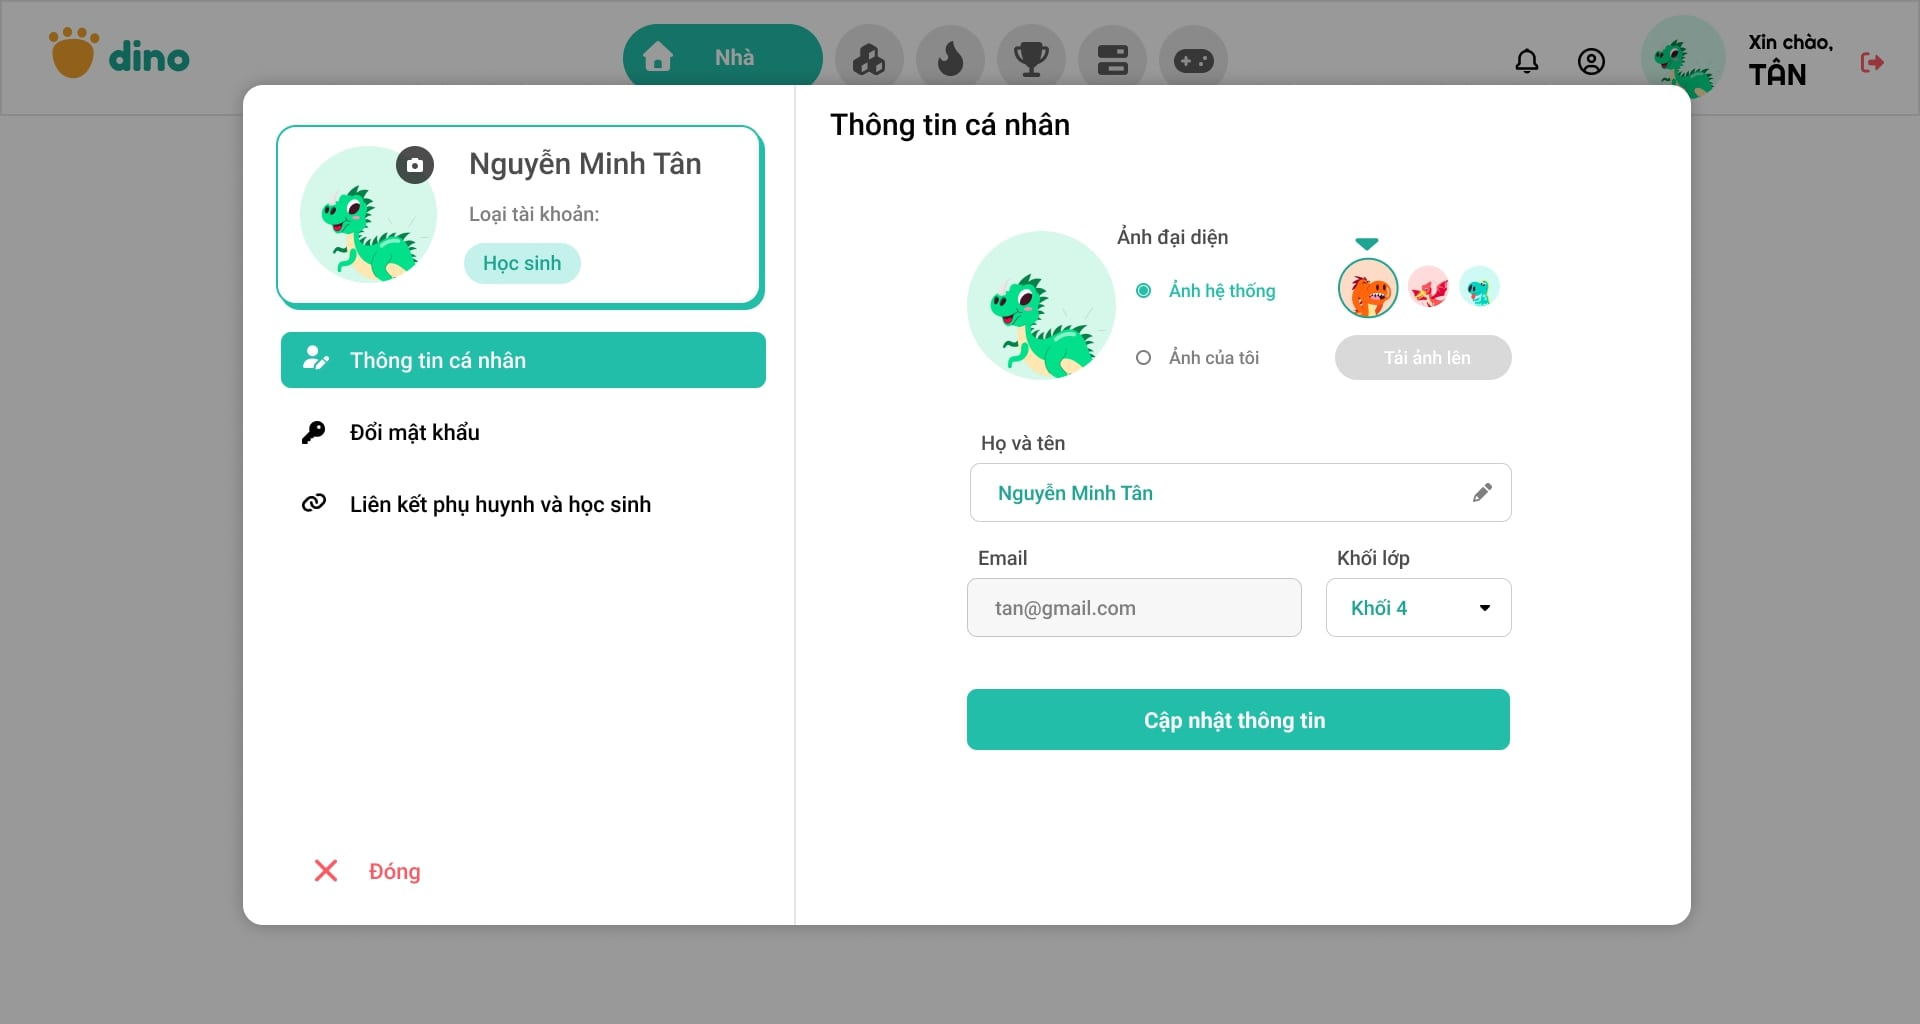
\includegraphics[width=0.9\textwidth]{Image/UI/Main-Student/Info.jpg}
		\vspace{0.6cm}
		\caption{Quản lý tài khoản cá nhân - Xem và cập nhật thông tin}
	\end{figure}

\item \textbf{Thay đổi mật khẩu}
\vspace{0.1cm}
\newline	
Học sinh có thể thay đổi mật khẩu bằng cách nhập các thông tin như mật khẩu hiện tại, mật khẩu mới và xác nhận mật khẩu. Chỉ có thể thay đổi mật khẩu khi các thông tin trên thỏa mãn các điều kiện sau:
		\begin{itemize}
			\item Giá trị của tất cả các field khác rỗng.
			\item Giá trị của field mật khẩu hiện tại phải trùng khớp.
			\item Mật khẩu có ít nhất 8 ký tự, trong đó phải chứa chữ cái in hoa, chữ thường, số và ký tự đặc biệt.
			\item Mật khẩu và Xác nhận mật khẩu phải trùng khớp. 
		\end{itemize}

		\begin{figure}[H]
			\centering
			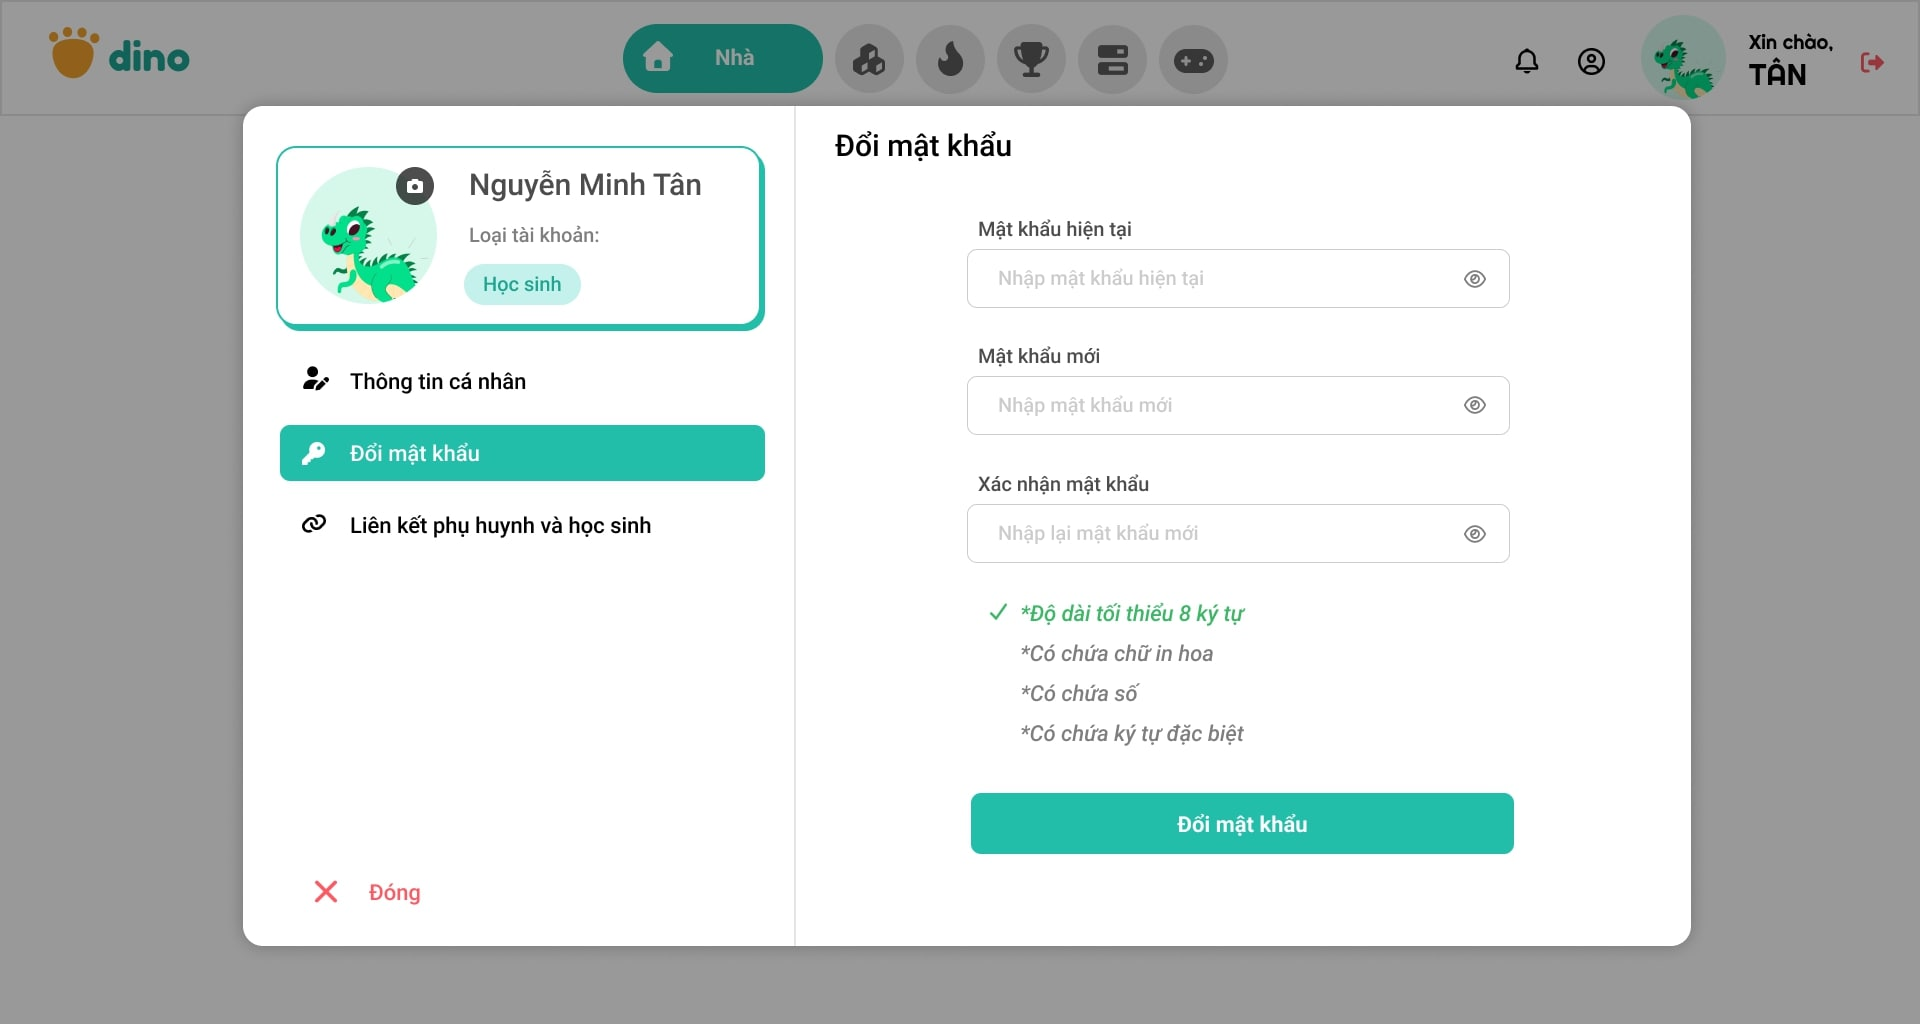
\includegraphics[width=0.9\textwidth]{Image/UI/Main-Student/ChangePassword.jpg}
			\vspace{0.6cm}
			\caption{Quản lý tài khoản cá nhân - Thay đổi mật khẩu}
		\end{figure}

	
\item \textbf{Liên kết tài khoản}
\vspace{0.1cm}
\newline
Tại giao diện này, học sinh có thể xem mã liên kết (mã mời) của Family hiện tại và có thể chia sẻ cho các học sinh khác. Ngoài ra, học sinh còn có thể xem đươc phụ huynh nào đang quản lý Family của mình.
		\begin{figure}[H]
			\centering
			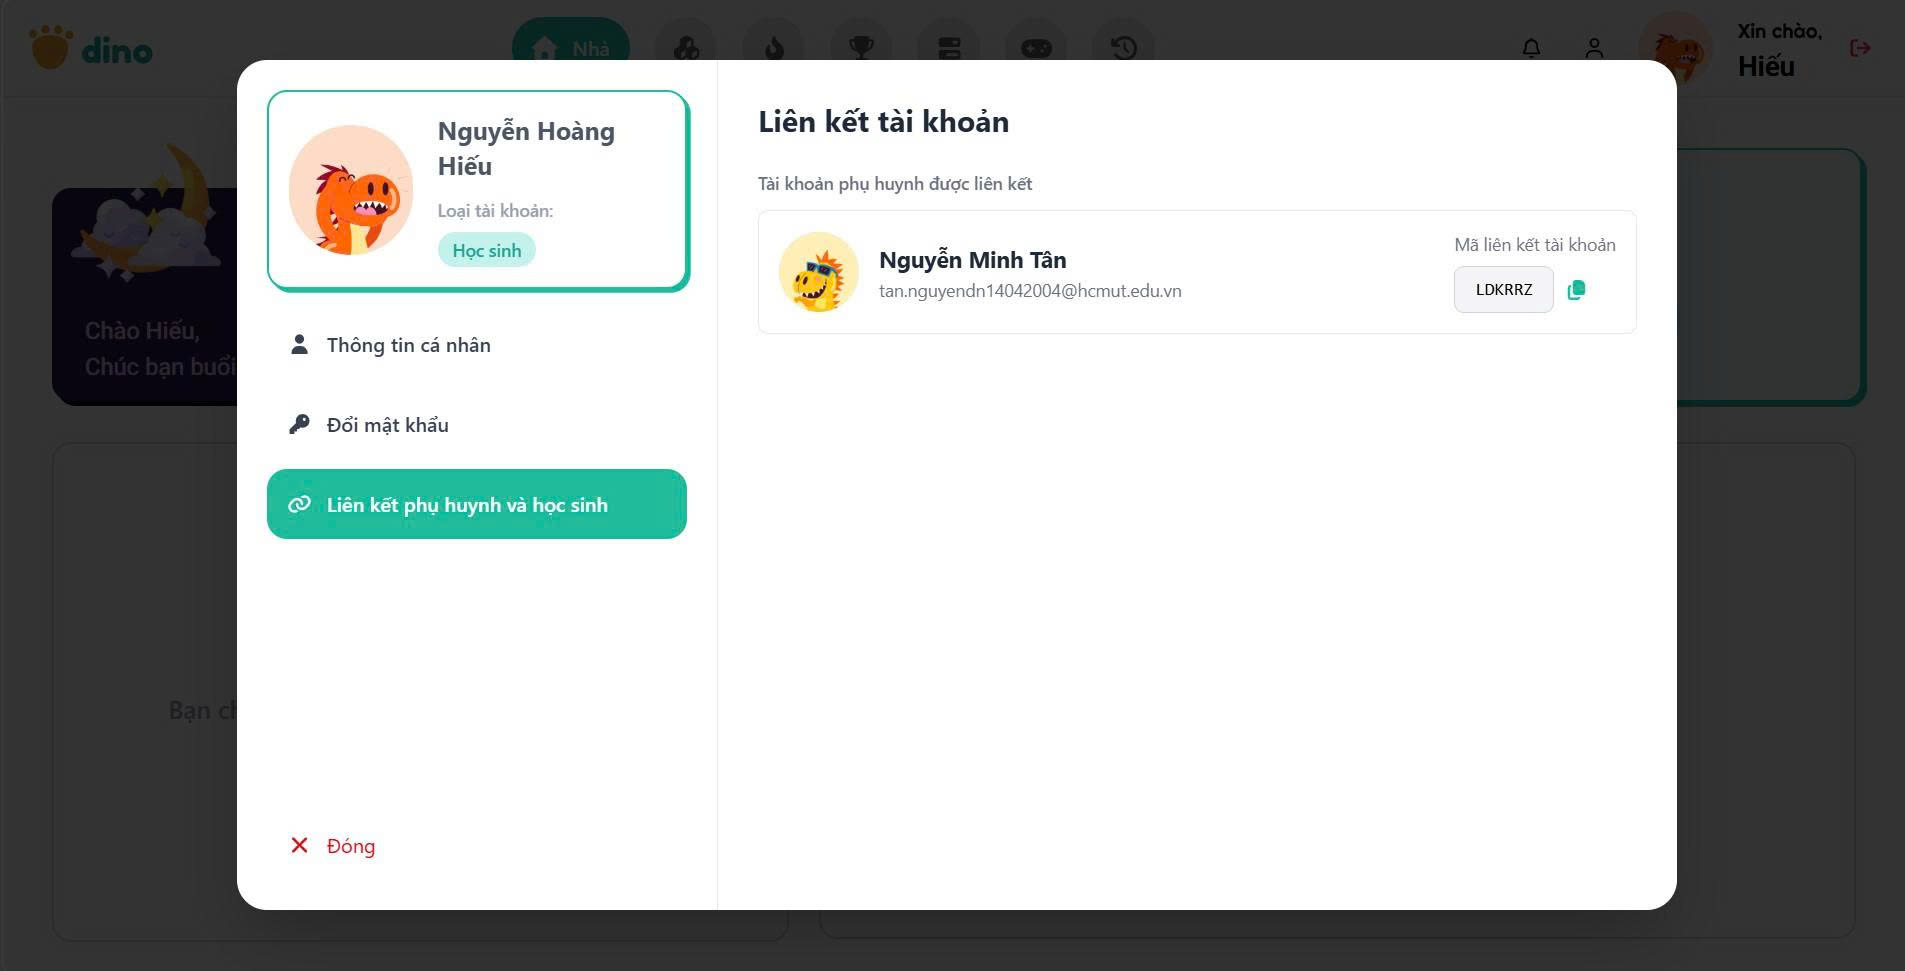
\includegraphics[width=0.9\textwidth]{Image/UI/Main-Student/Account-Linked.jpg}
			\vspace{0.6cm}
			\caption{Quản lý tài khoản cá nhân - Đã liên kết tài khoản}
		\end{figure}
\end{enumerate}

\subsection{Các màn hình chính của tài khoản Phụ huynh}
\subsubsection{Trang Thống kê tổng quan}
\label{subsubsec:parenthome}
Mỗi phụ huynh sẽ là quản trị viên của một Family và có thể quản lý nhiều học sinh khác nhau. Vì thế, ở phần bộ lọc bên trái, ngoài lọc theo thời gian còn có lọc theo học sinh. Ở phần nội dung giữa màn hình, phụ huynh có thể xem các thống kê tổng quan về học tập và đấu trường của học sinh được chọn.
	\begin{figure}[H]
		\centering
		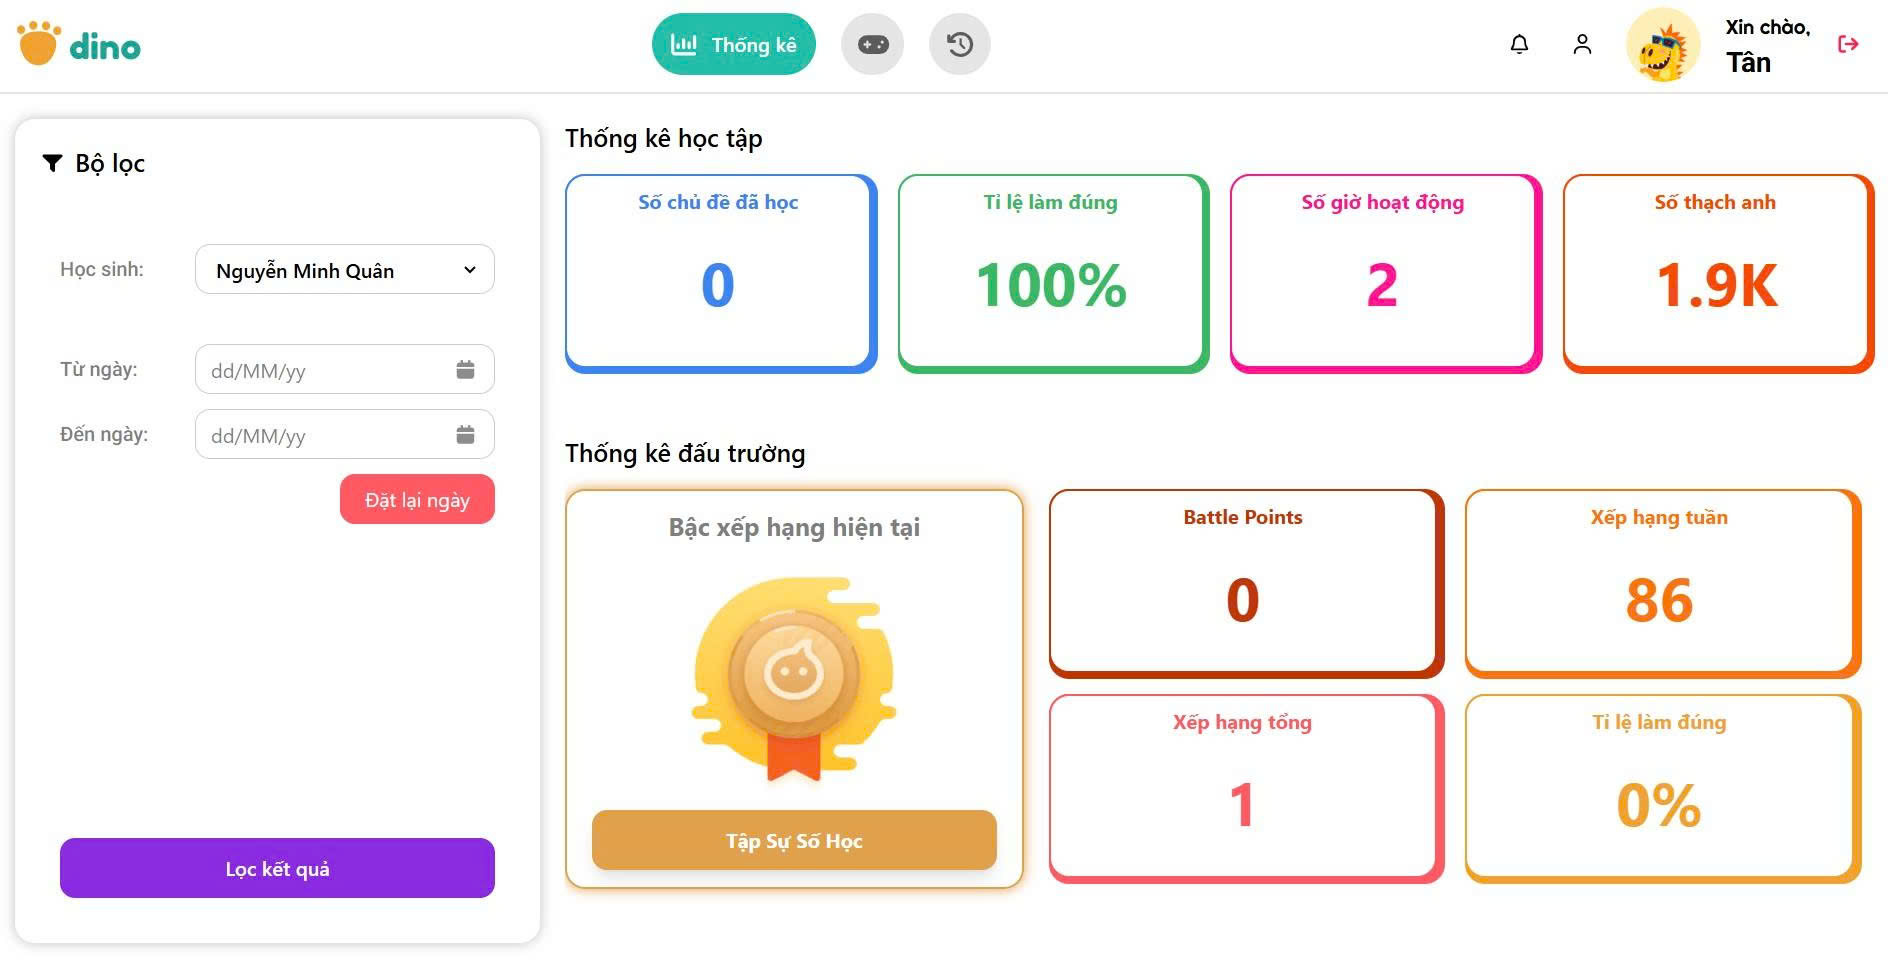
\includegraphics[width=0.9\textwidth]{Image/UI/Main-Parent/Statistics.jpg}
		\vspace{0.6cm}
		\caption{Thống kê tổng quan}
	\end{figure}


\subsubsection{Trang Lịch sử bài làm}
Phụ huynh có thể xem lịch sử các lần làm bài của học sinh, xem thống kê tổng quan về số bài tập đã làm và tỉ lệ làm đúng trung bình. Phụ huynh có thể thay đổi bộ lọc ở bên trái để dễ dàng lọc các bản ghi. Trên mỗi bản ghi có hiển thị thông tin về tên bài tập, thời gian làm bài, thời gian kết thúc, số câu đúng và đánh giá mức độ bằng số sao và màu sắc. Giao diện lịch sử làm bài của phụ huynh được thiết kế như hình bên dưới.
\begin{figure}[H]
 	\centering
 	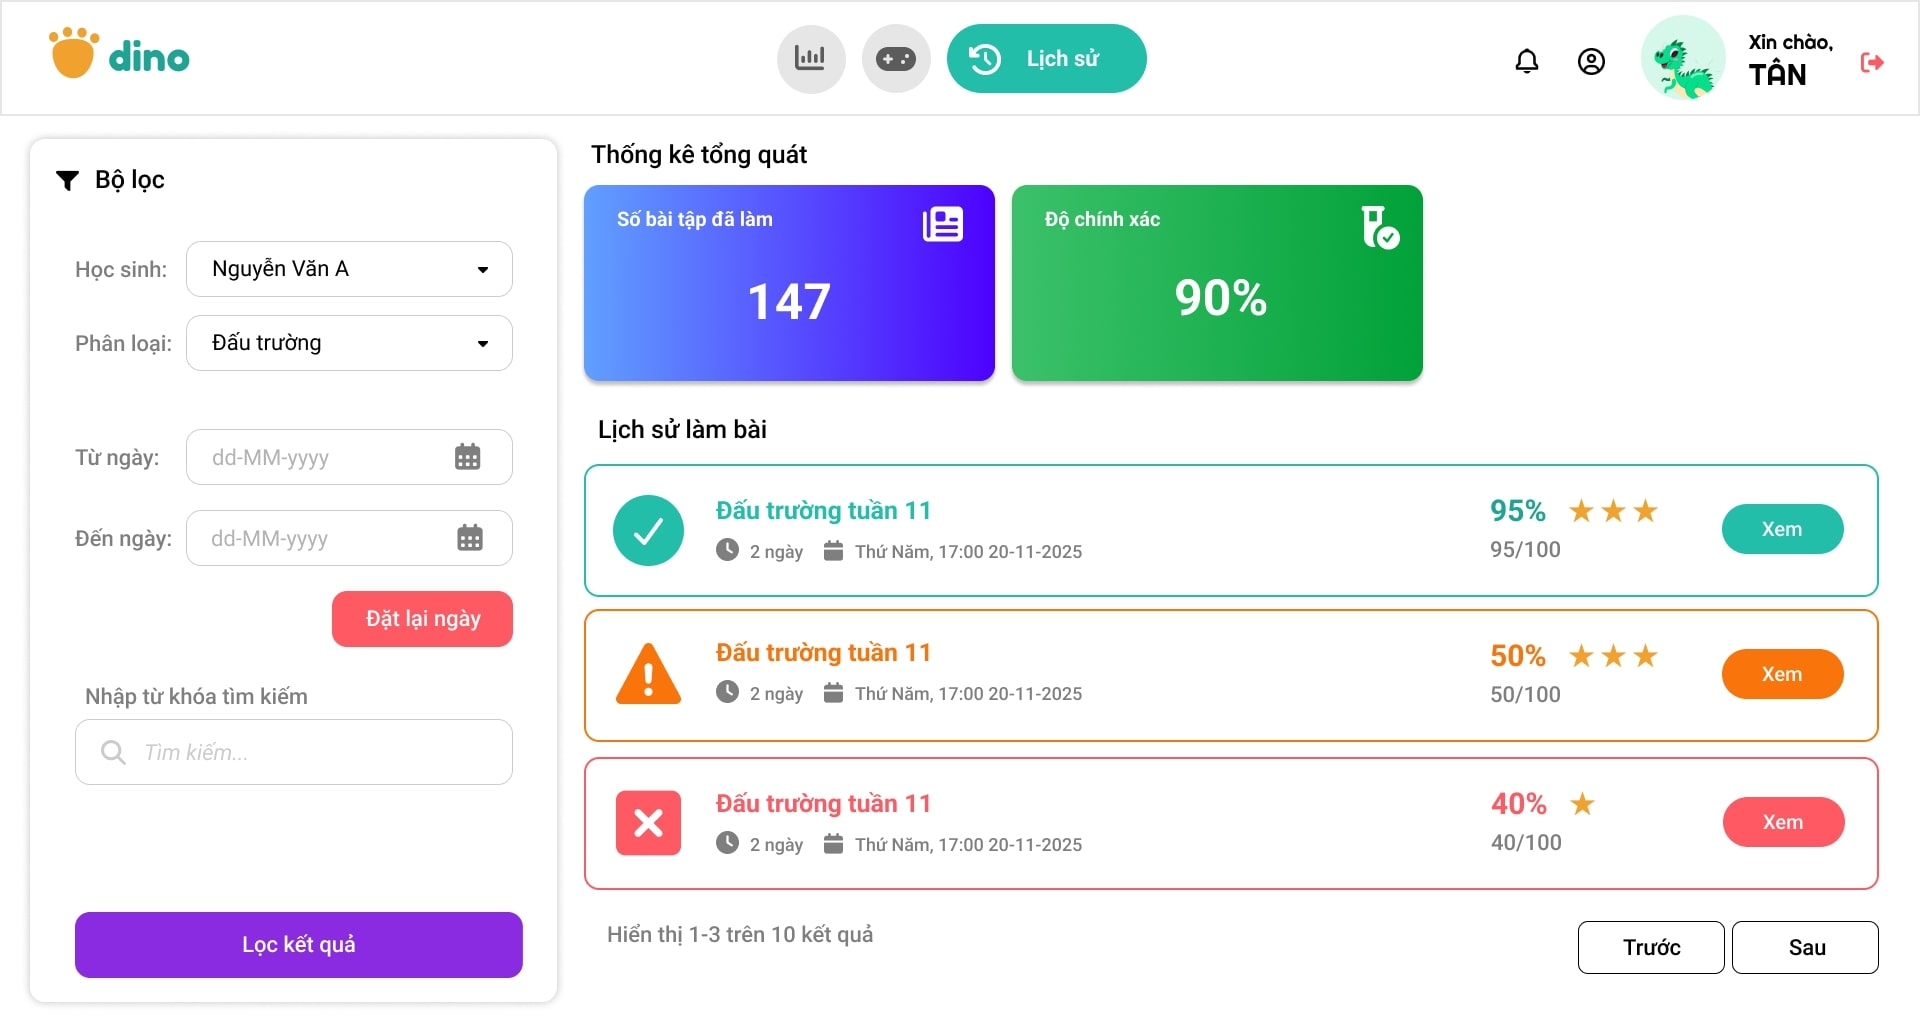
\includegraphics[width=0.9\textwidth]{Image/UI/Main-Parent/History.jpg}
 	\vspace{0.6cm}
 	\caption{Lịch sử làm bài}
 \end{figure}
 
\vspace{0.2cm}
\newline
Phụ huynh còn có thể xem chi tiết bài làm của học sinh bằng cách bấm vào nút \textit{Xem} trên mỗi bản ghi. Trang chi tiết bài làm bao gồm thông tin tổng quan của bài làm (tên học sinh, lớp, thời gian hoàn thành, thời gian làm bài, tổng số câu, số câu đúng/sai). Ngoài ra, phụ huynh có thể đánh giá năng lực của con thông qua chi tiết các câu trả lời. Giao diện chi tiết bài làm được thiết kế như hình dưới đây.
	\begin{figure}[H]
		\centering
		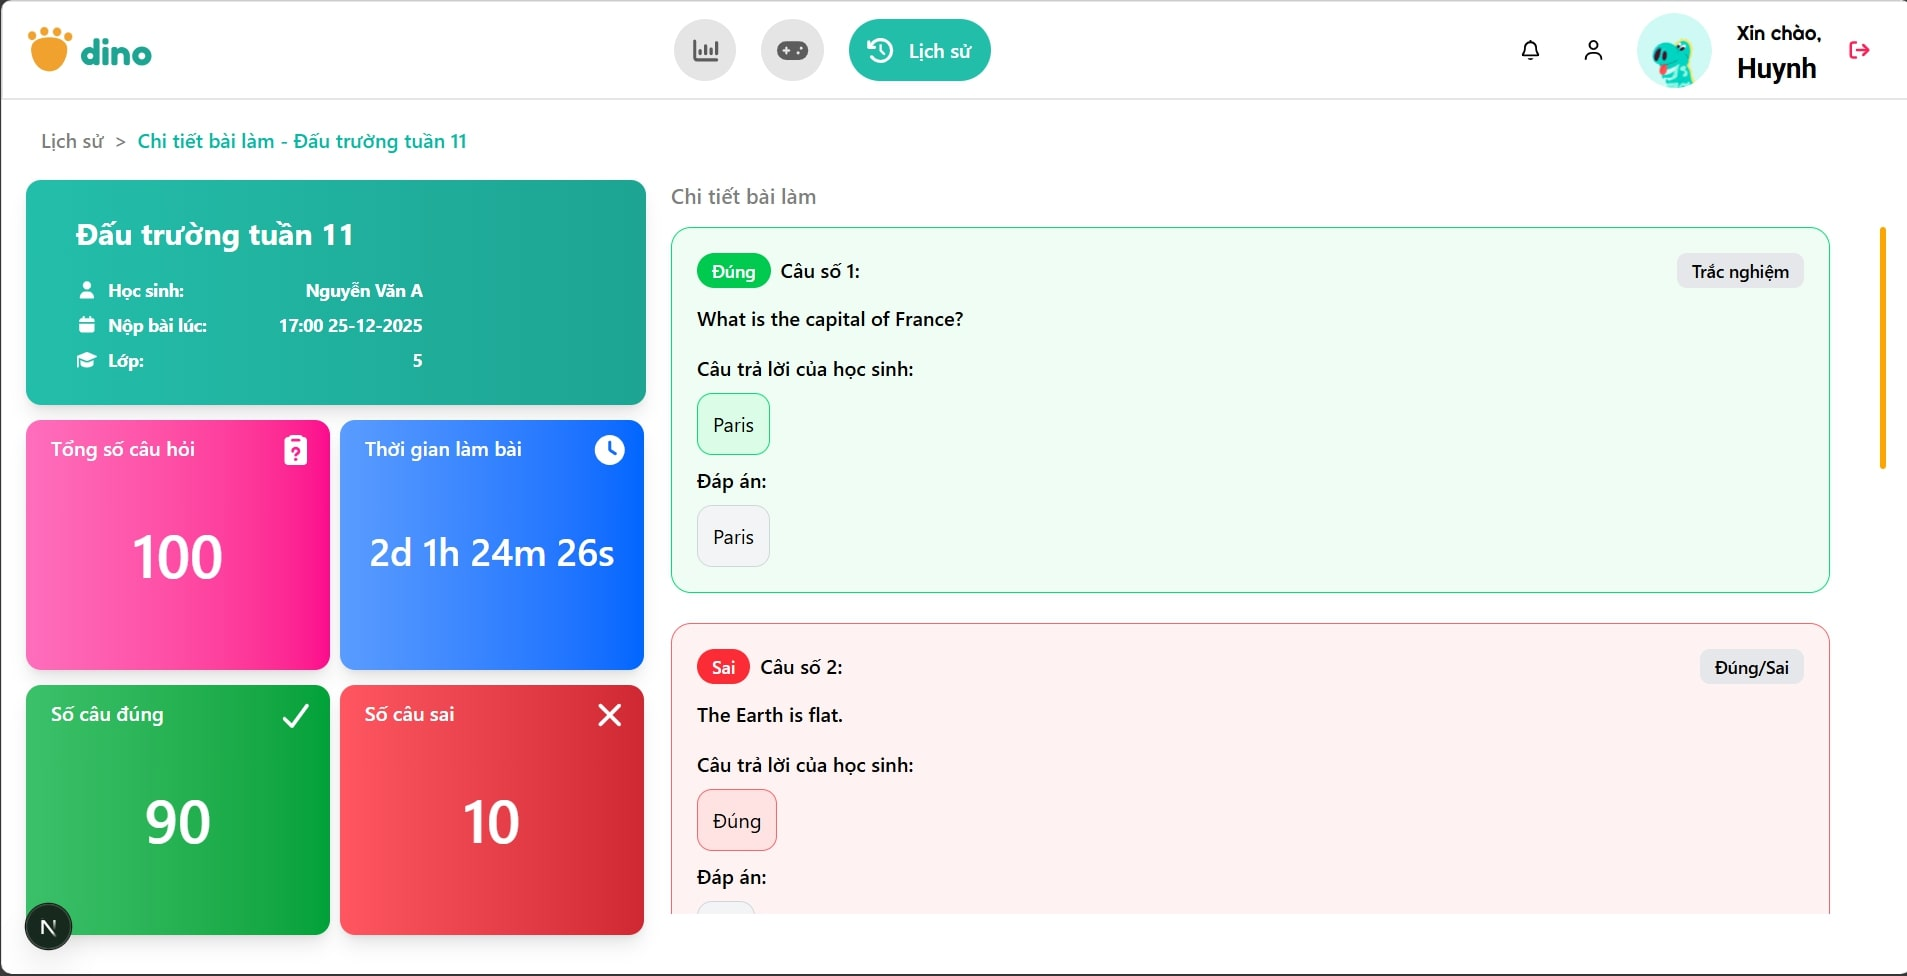
\includegraphics[width=0.9\textwidth]{Image/UI/Main-Parent/ExamDetail.jpg}
		\vspace{0.6cm}
		\caption{Chi tiết bài làm}
	\end{figure}

\subsubsection{Trang Minigames}
Trang Minigames của phụ huynh được thiết kế tương tự với Trang Minigames của Học sinh. Thiết kế được mô tả chi tiết ở mục \ref{subsubsec:games}.

\subsubsection{Quản lý tài khoản cá nhân}
\begin{enumerate}
	\item \textbf{Xem và cập nhật thông tin cá nhân}
	\vspace{0.1cm}
	\newline
	Phụ huynh có thể xem và chỉnh sửa thông tin cá nhân, bao gồm ảnh đại diện, họ và tên. Tuy nhiên, email là cố định với mỗi tài khoản và chỉ được quyền xem.
		\begin{figure}[H]
			\centering
			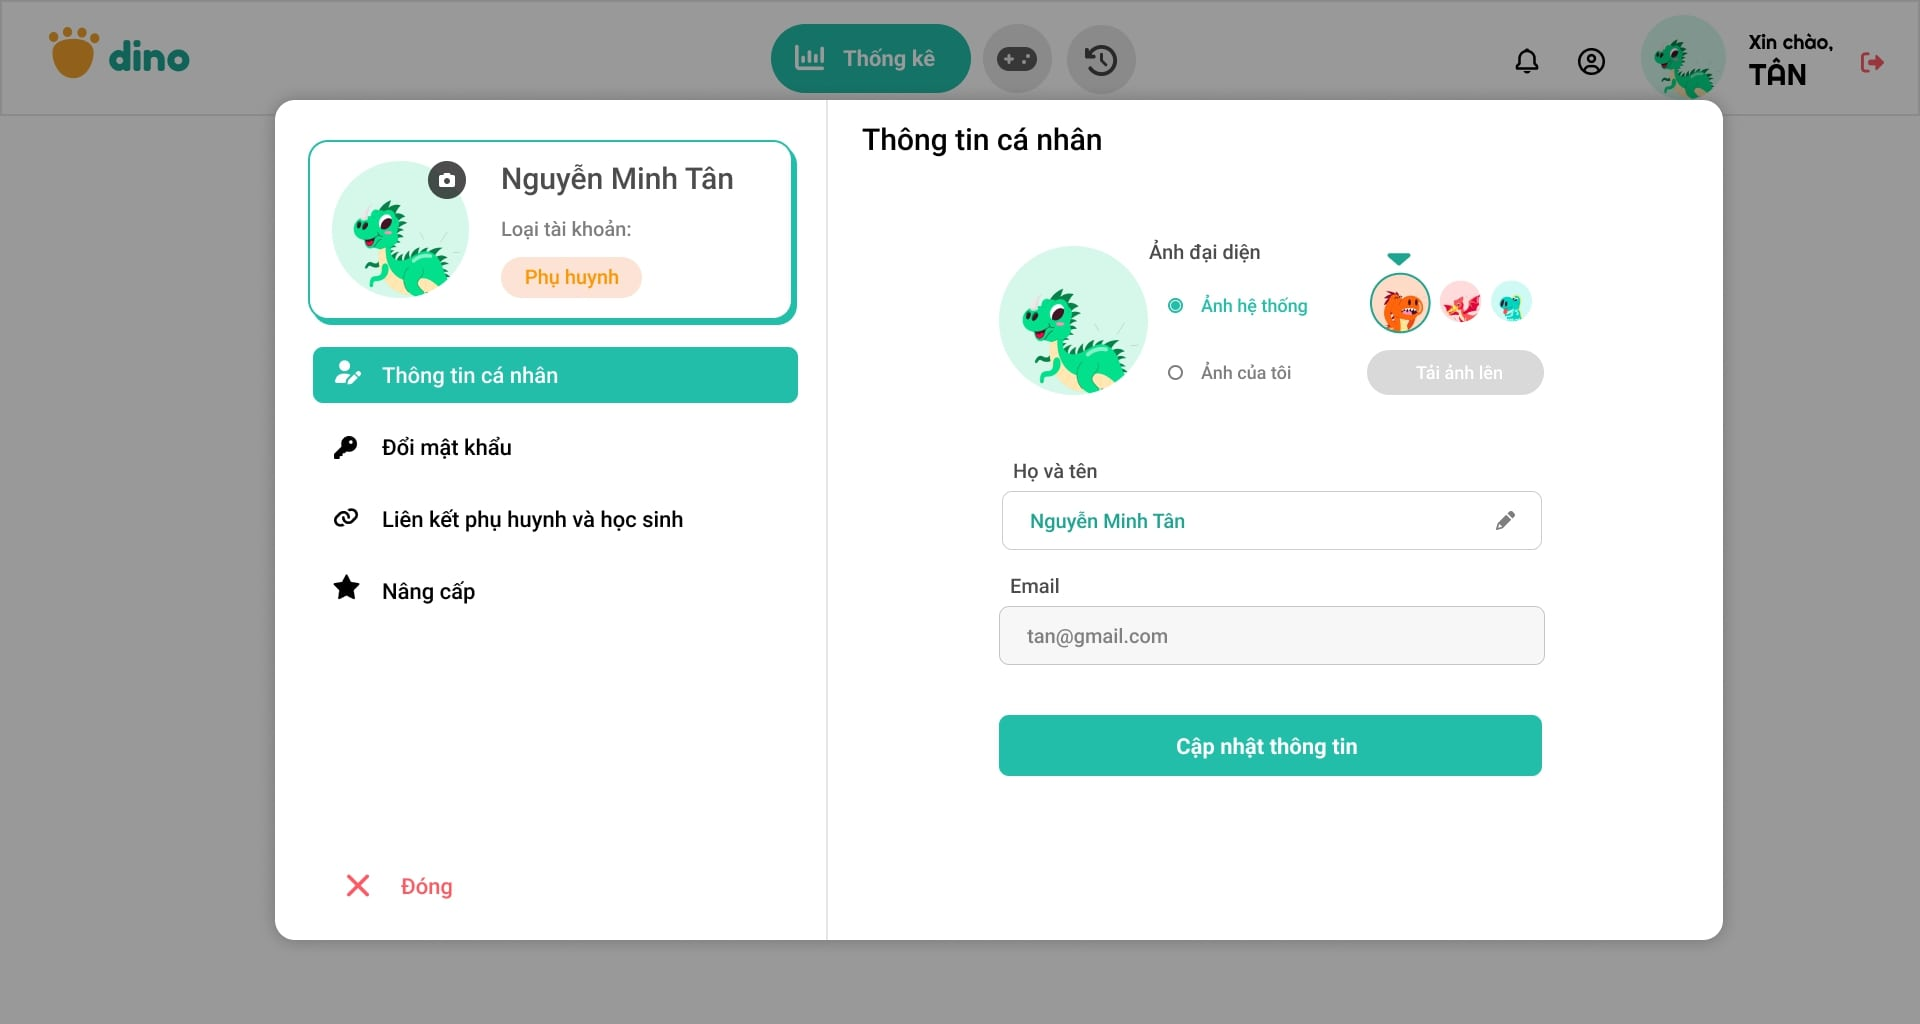
\includegraphics[width=0.9\textwidth]{Image/UI/Main-Parent/Info.jpg}
			\vspace{0.6cm}
			\caption{Quản lý tài khoản cá nhân - Xem và cập nhật thông tin}
		\end{figure}
	
	\item \textbf{Thay đổi mật khẩu}: Giao diện thay đổi mật khẩu của phụ huynh được thiết kế tương tự với giao diện của Học sinh. Thiết kế được mô tả chi tiết ở mục \ref{subsubsec:profile}.
	\newpage
	\item \textbf{Liên kết tài khoản}
	\vspace{0.1cm}
	\newline
		Phụ huynh có thể xem danh sách các tài khoản học sinh đã được liên kết vào Family như \textit{Hình \ref{fig:linked}}.
		\begin{figure}[H]
			\centering
			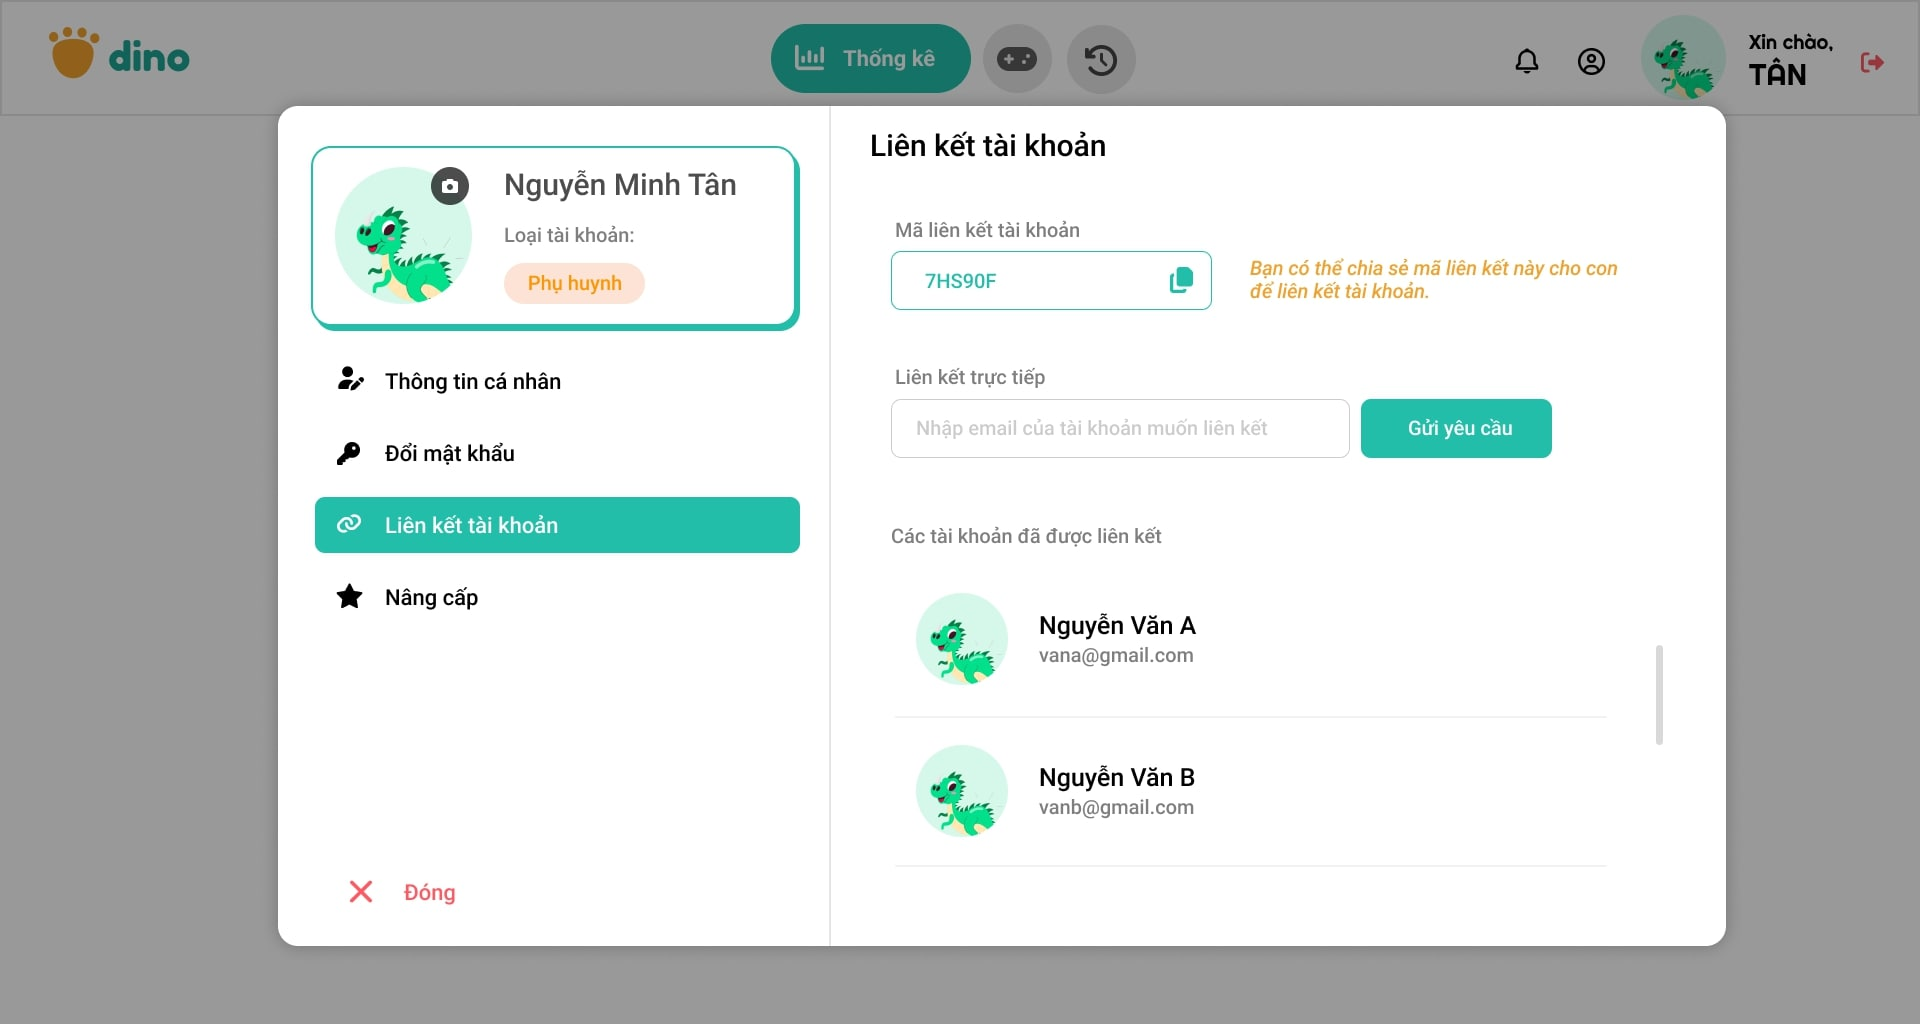
\includegraphics[width=0.9\textwidth]{Image/UI/Main-Parent/Account-Linked.jpg}
			\vspace{0.6cm}
			\caption{Quản lý tài khoản cá nhân - Đã liên kết tài khoản}
			\label{fig:linked}
		\end{figure}
	
	\item \textbf{Nâng cấp tài khoản}
	\vspace{0.1cm}
	\newline
	Phụ huynh có thể nâng cấp tài khoản qua các bước sau:
		\begin{itemize}
			\item Bước 1: Chọn Gói nâng cấp muốn mua.
			\begin{figure}[H]
				\centering
				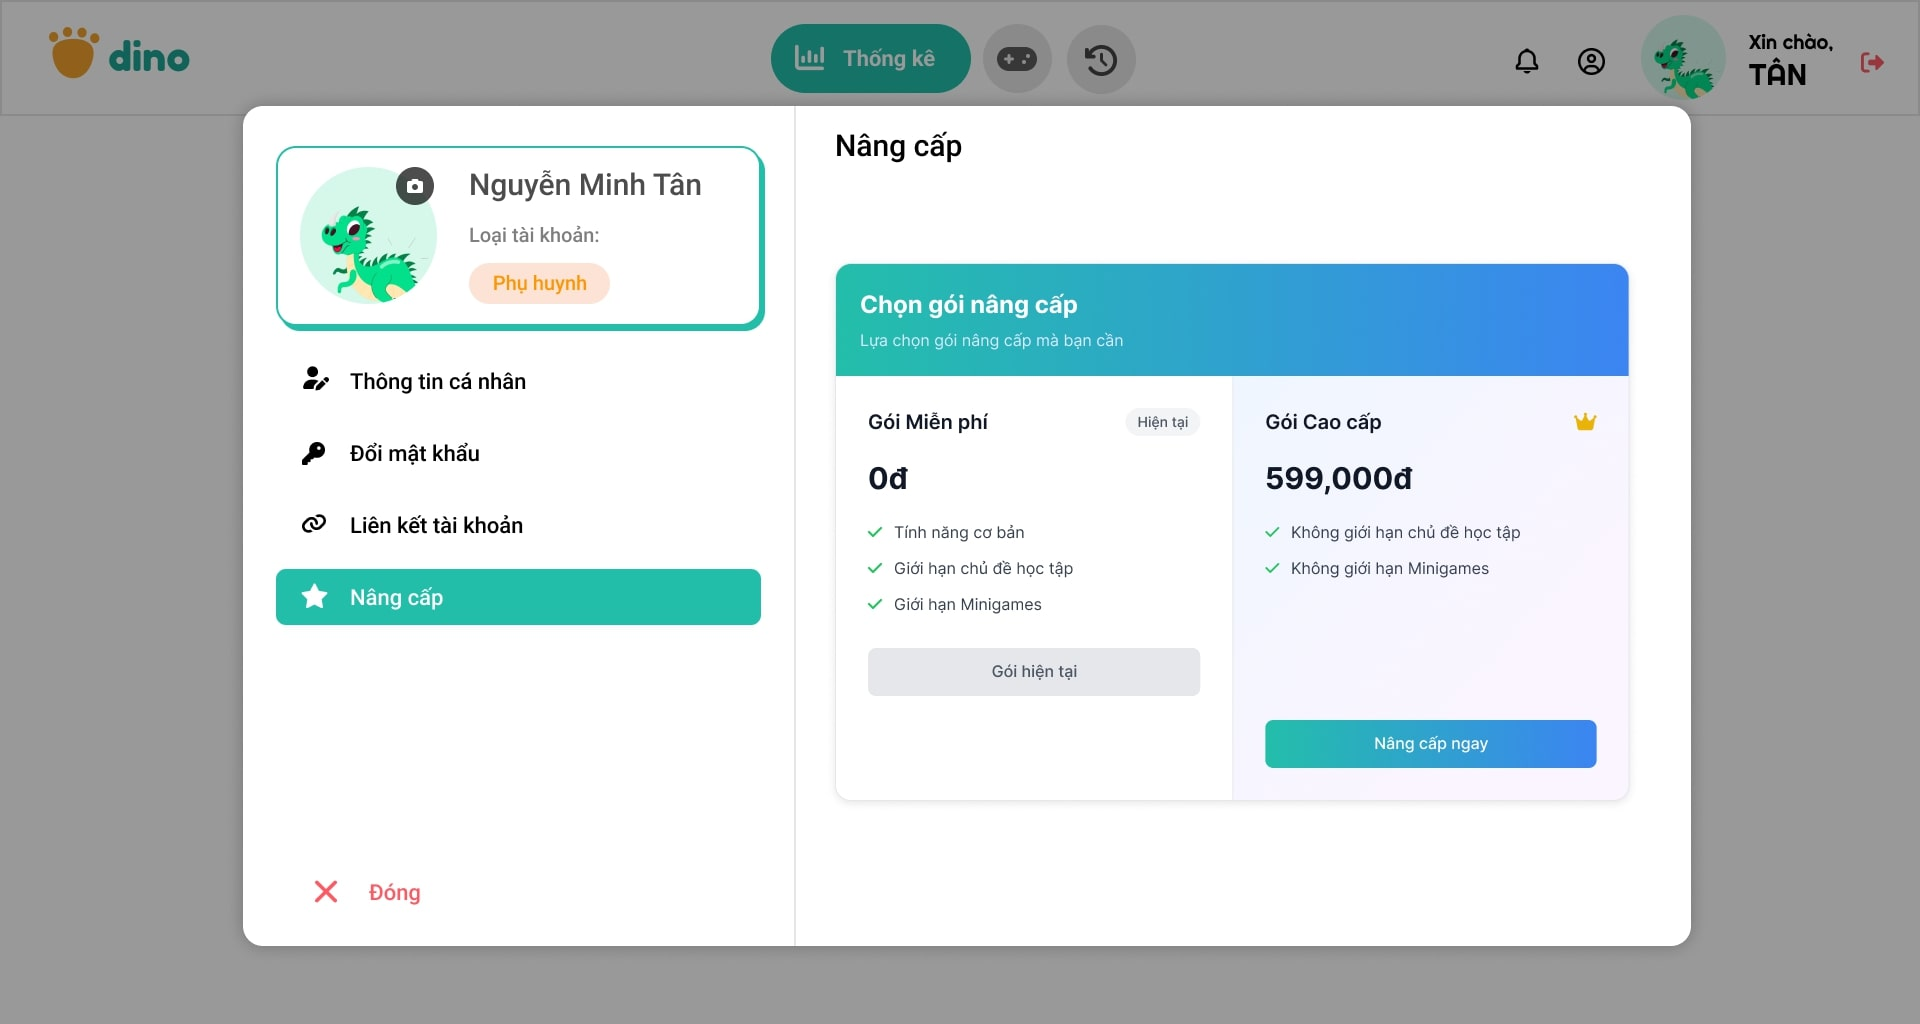
\includegraphics[width=0.9\textwidth]{Image/UI/Main-Parent/Plans.jpg}
				\vspace{0.6cm}
				\caption{Các gói nâng cấp}
			\end{figure}
			
			\item Bước 2: Thanh toán qua QRCode của VNPay.
			\begin{figure}[H]
				\centering
				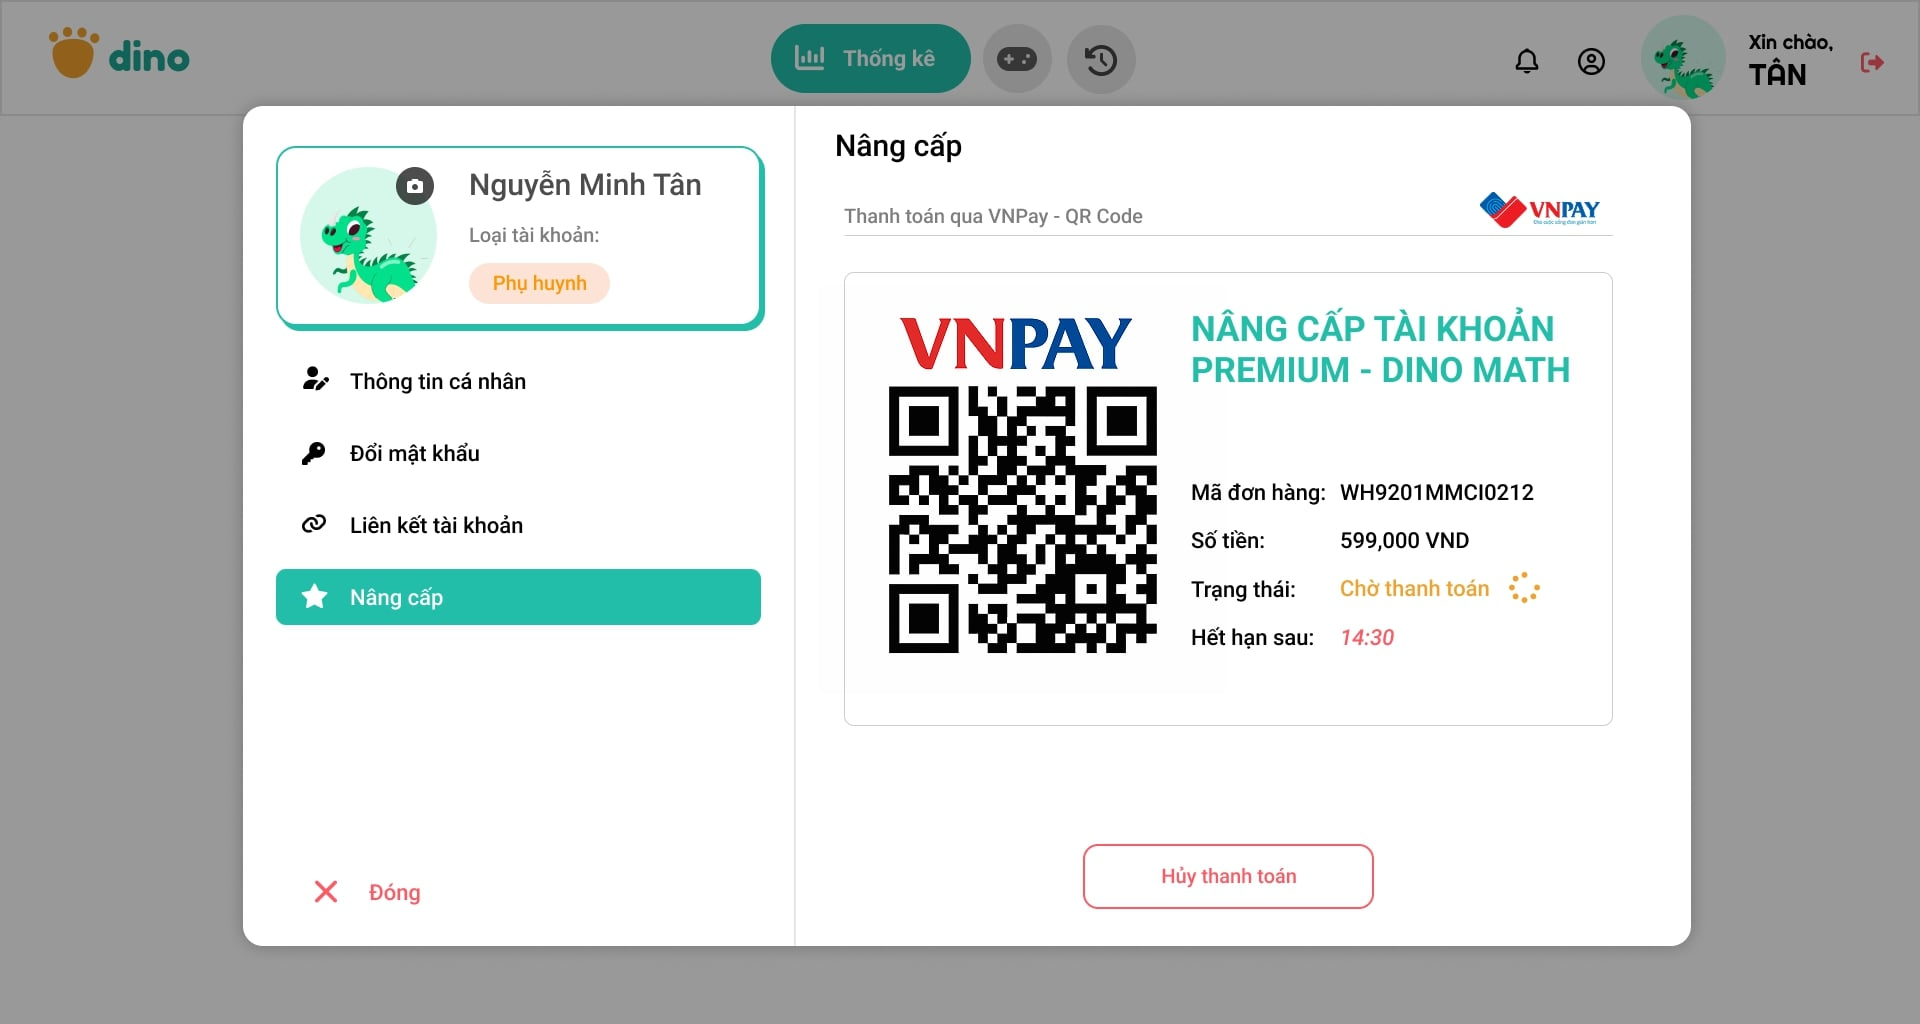
\includegraphics[width=0.9\textwidth]{Image/UI/Main-Parent/Payment-Loading.jpg}
				\vspace{0.6cm}
				\caption{Chờ xác nhận thanh toán}
			\end{figure}
			
			\item Bước 3: Sau khi thanh toán thành công, màn hình hiển thị trạng thái tài khoản đã nâng cấp và một số các phúc lợi của người dùng.
			\begin{figure}[H]
				\centering
				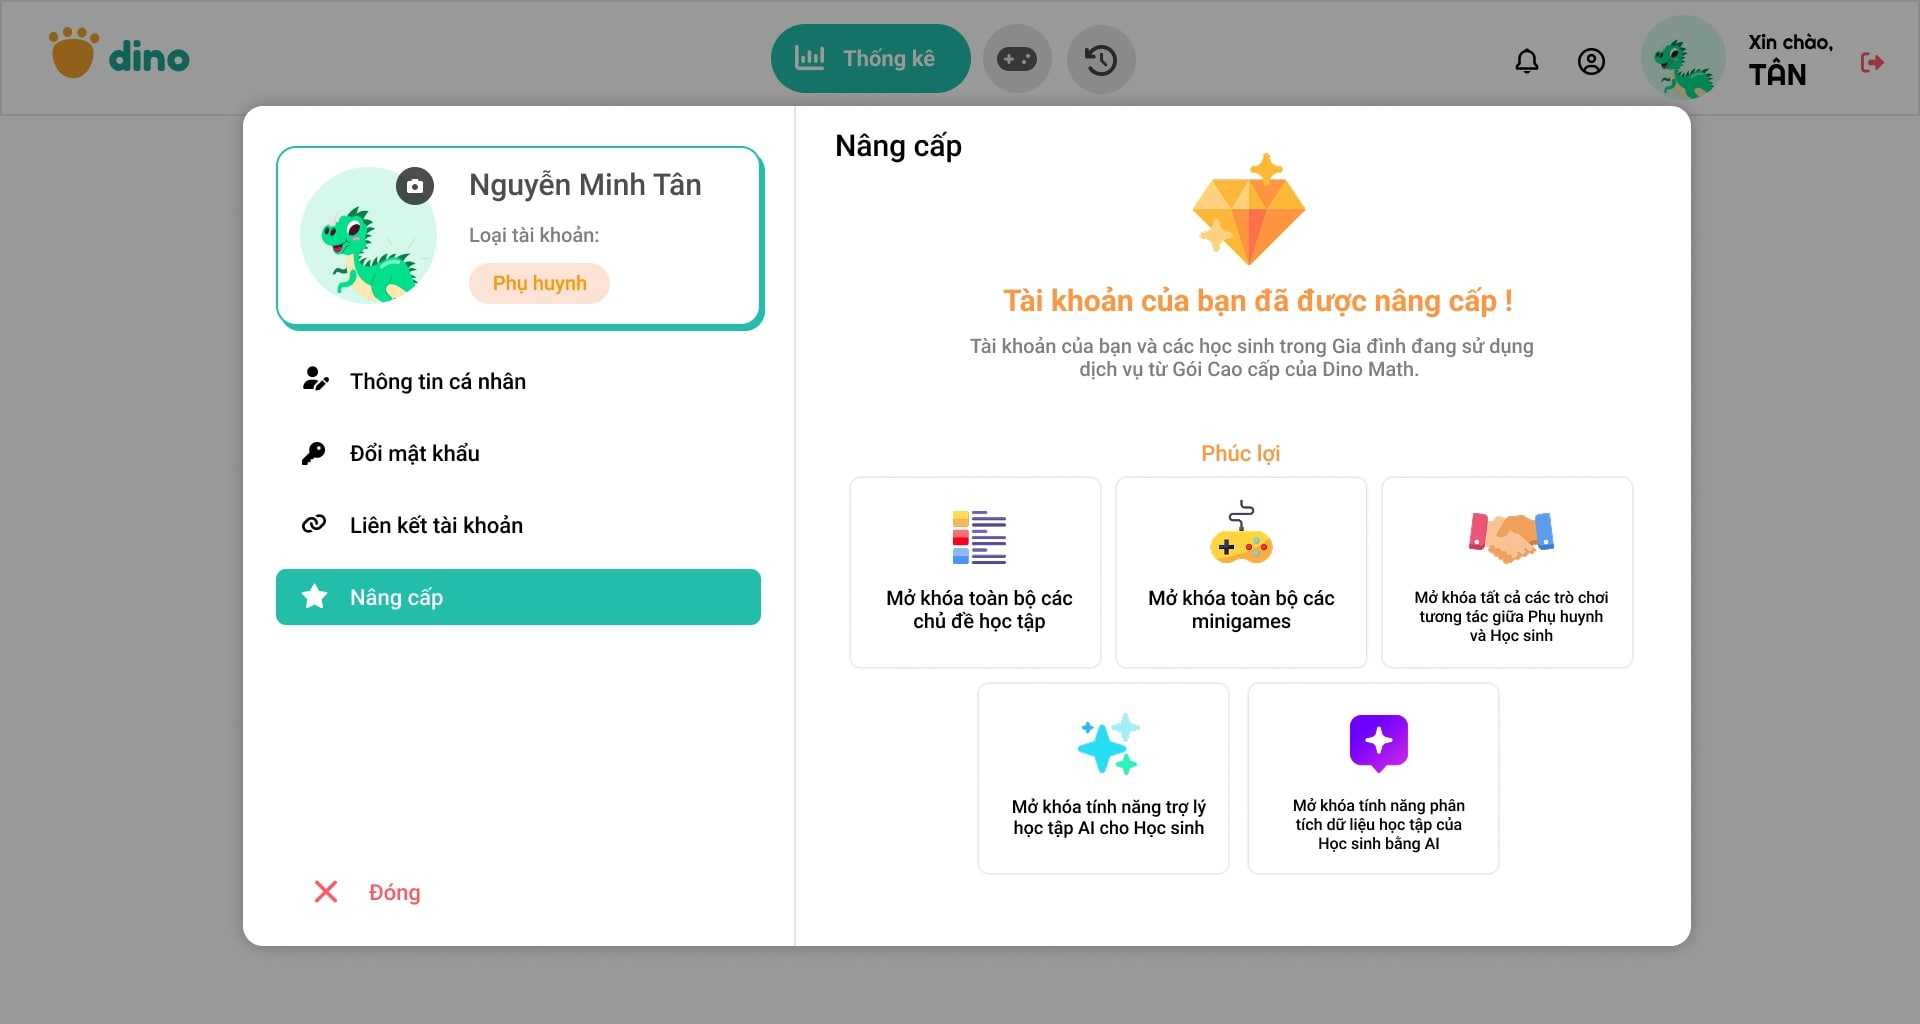
\includegraphics[width=0.9\textwidth]{Image/UI/Main-Parent/AfterPurchase.jpg}
				\vspace{0.6cm}
				\caption{Trạng thái tài khoản đã được nâng cấp}
			\end{figure}
		\end{itemize}
\end{enumerate}

\subsection{Các màn hình chính của quản trị viên (Admin)}

\subsubsection{Quản lý tài khoản}
Quản trị viên có thể xem danh sách tài khoản người dùng và thực hiện khoá hoặc mở khoá tài khoản.
\begin{figure}[H]
	\centering
	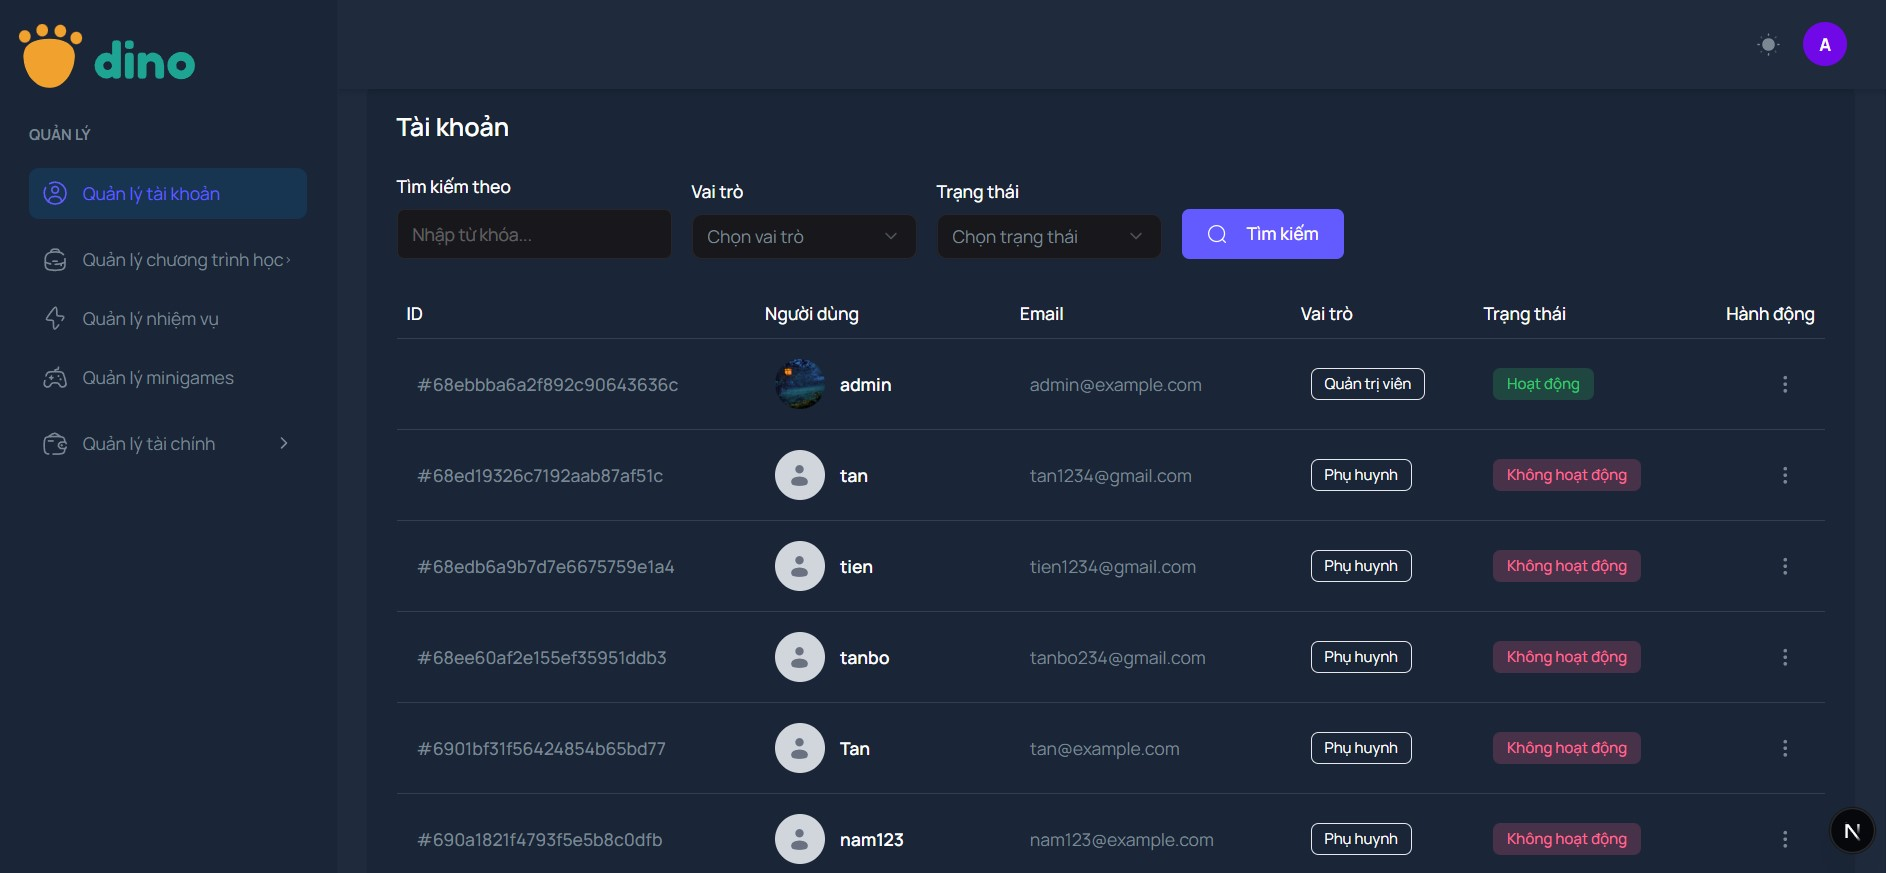
\includegraphics[width=0.9\textwidth]{Image/UI/Admin/Account.jpg}
	\vspace{0.6cm}
	\caption{Admin - Quản lý tài khoản}
\end{figure}

\subsubsection{Quản lý học kỳ}
Quản trị viên có thể tạo và quản lý các học kỳ trong năm học, làm cơ sở để gắn kết bài kiểm tra đầu vào và các hoạt động theo từng giai đoạn học tập.
\begin{figure}[H]
	\centering
	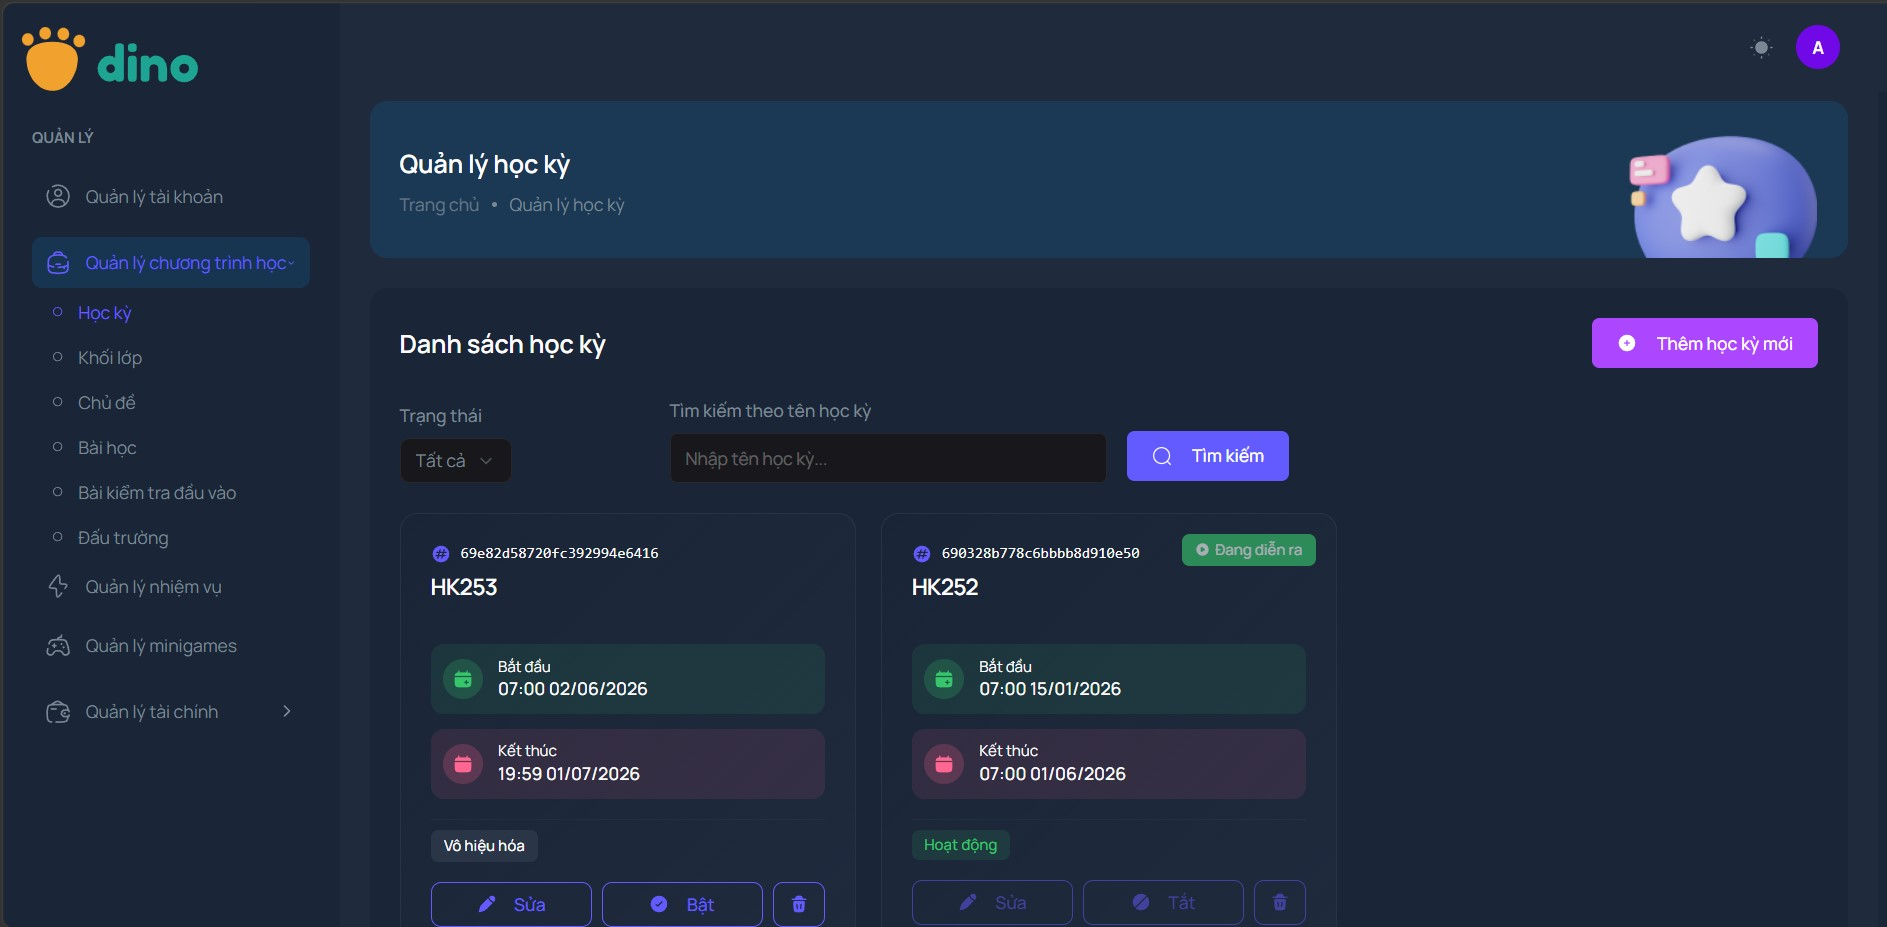
\includegraphics[width=0.9\textwidth]{Image/UI/Admin/Semester.jpg}
	\vspace{0.6cm}
	\caption{Admin - Quản lý học kỳ}
\end{figure}

\subsubsection{Quản lý khối lớp}
Quản trị viên có thể xem và chỉnh sửa các khối lớp (Lớp 1--5). Mỗi khối lớp gắn liền với một thế giới riêng, trong đó bao gồm các vùng đất tương ứng với từng chủ đề học.
\begin{figure}[H]
	\centering
	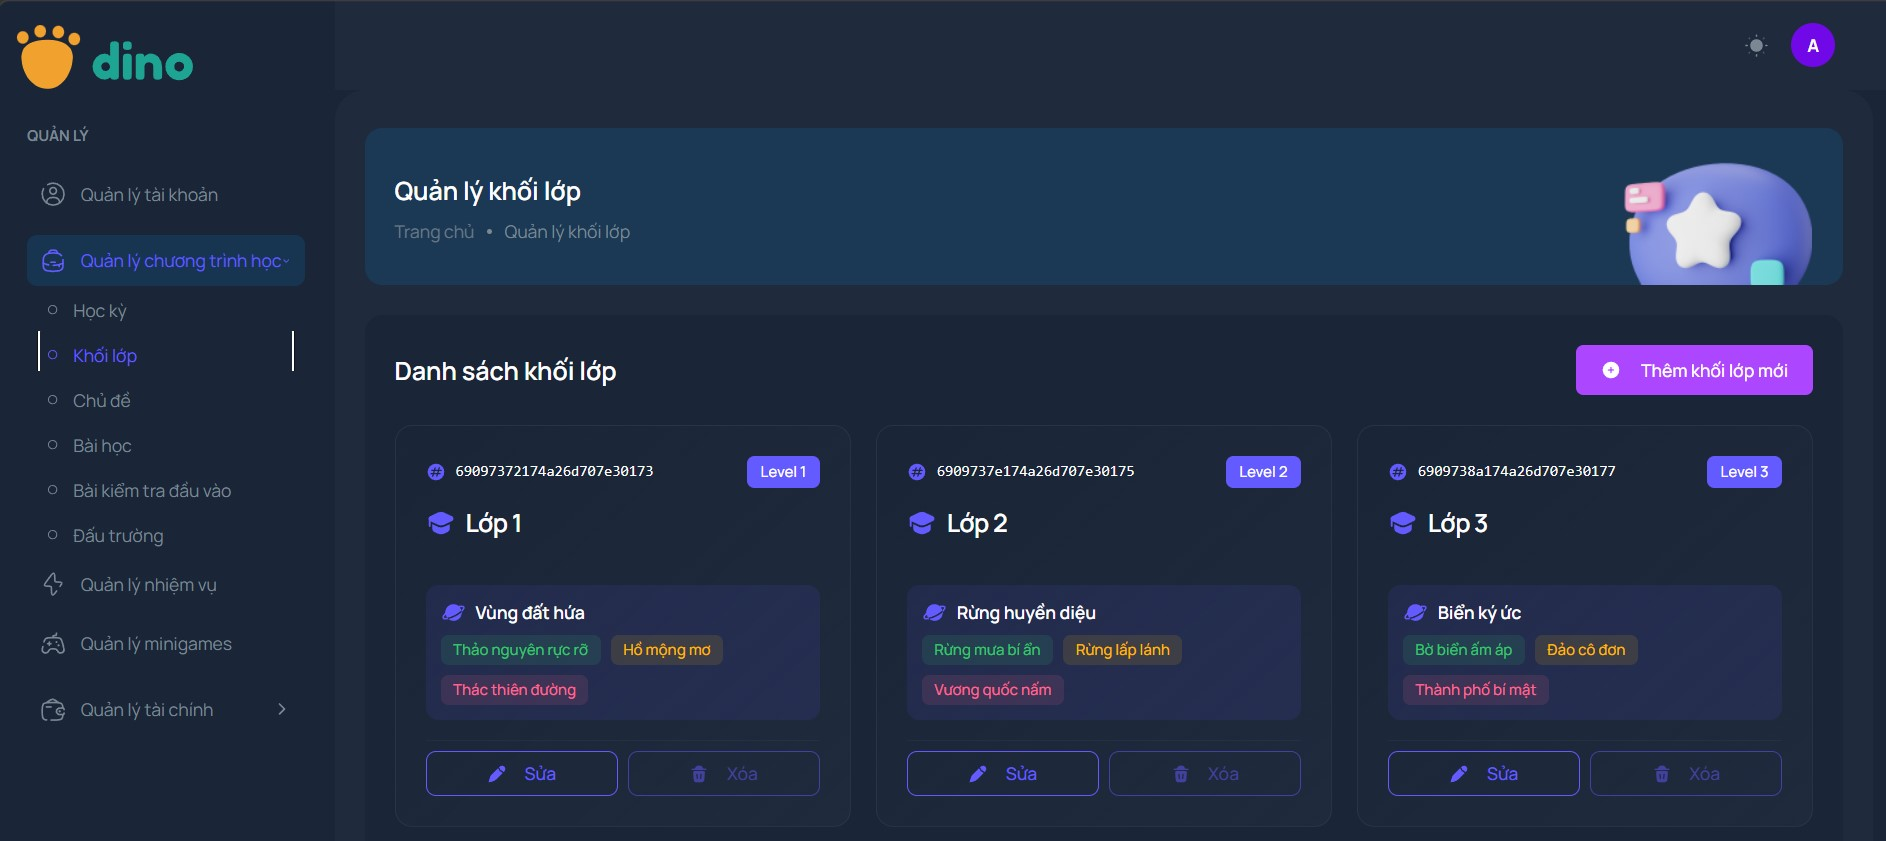
\includegraphics[width=0.9\textwidth]{Image/UI/Admin/Grade.jpg}
	\vspace{0.6cm}
	\caption{Admin - Quản lý khối lớp}
\end{figure}

\subsubsection{Quản lý bài học}
Quản trị viên có thể xem, tìm kiếm và lọc danh sách bài học theo chủ đề và độ khó. Hệ thống hỗ trợ thêm mới bài học, xóa bài học theo chủ đề, và xuất định dạng Excel mẫu để nhập liệu hàng loạt.
\begin{figure}[H]
	\centering
	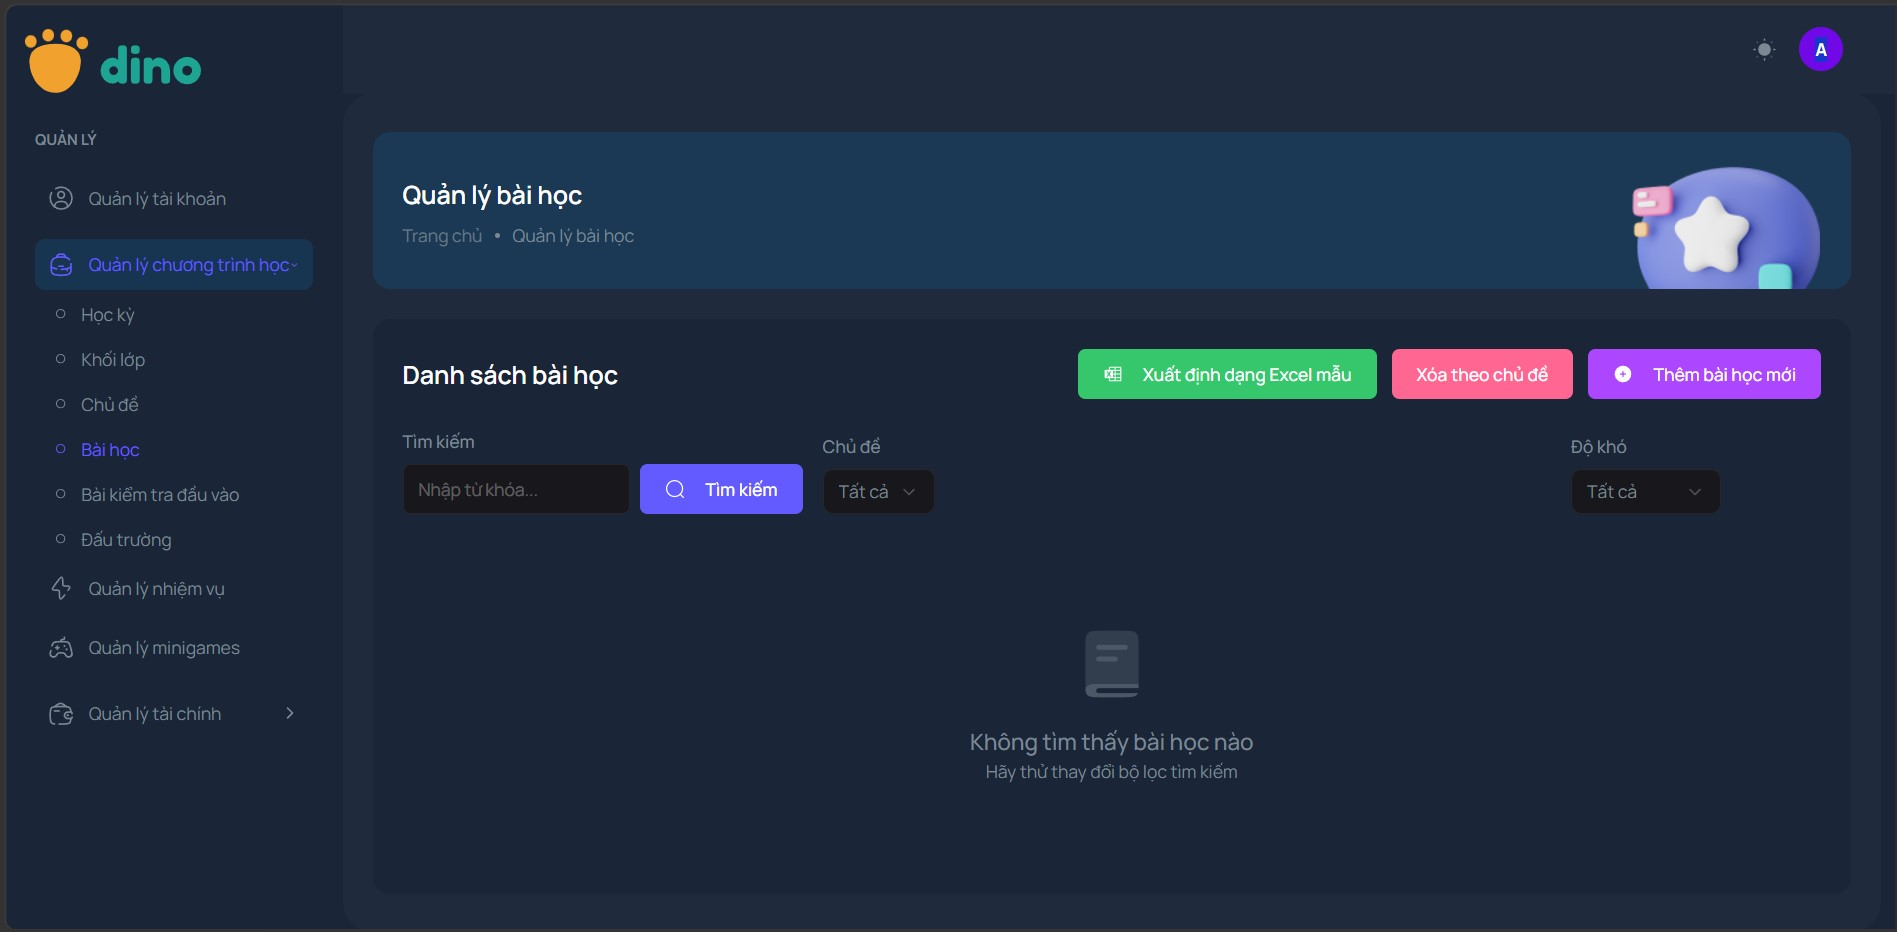
\includegraphics[width=0.9\textwidth]{Image/UI/Admin/Lesson.jpg}
	\vspace{0.6cm}
	\caption{Admin - Quản lý bài học}
\end{figure}

\subsubsection{Quản lý bài tập}
Quản trị viên có thể tạo, chỉnh sửa và xoá nội dung bài tập, tổ chức theo chủ đề và bài học.
\begin{figure}[H]
	\centering
	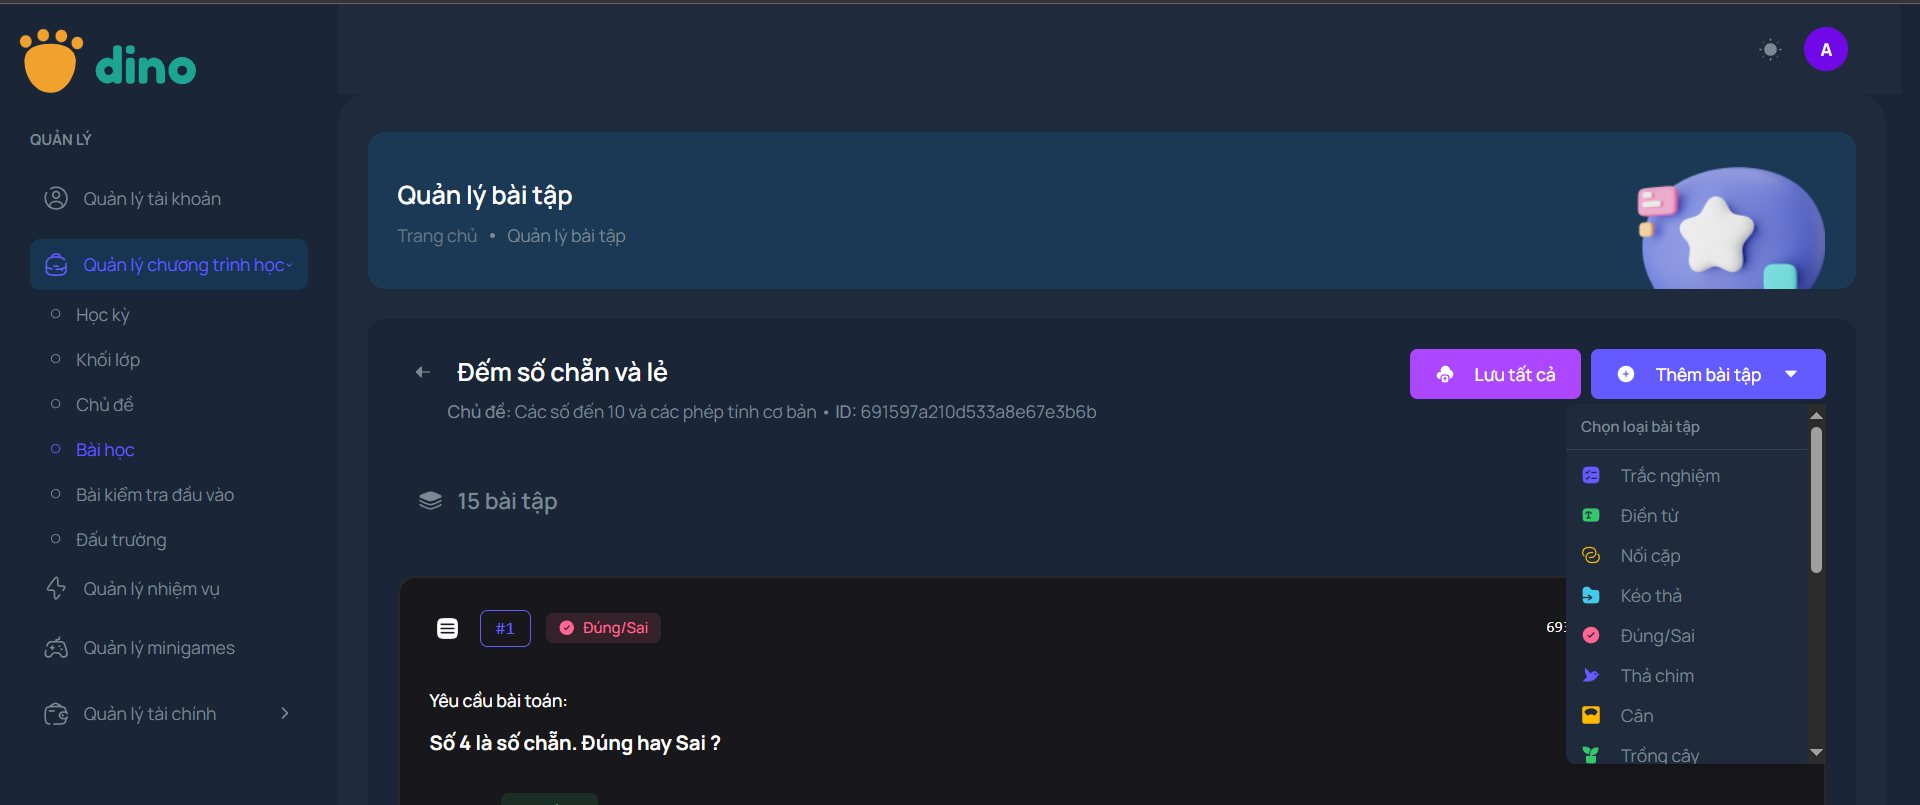
\includegraphics[width=0.9\textwidth]{Image/UI/Admin/Exercise.jpg}
	\vspace{0.6cm}
	\caption{Admin - Quản lý bài tập}
\end{figure}

Khi thêm mới hoặc chỉnh sửa bài tập, hệ thống cung cấp hai phương thức nhập liệu linh hoạt như sau:
\begin{itemize}
	\item \textbf{Nhập liệu qua form:} Mỗi dạng bài tập (trắc nghiệm, kéo thả, điền khuyết, nối, đúng/sai,...) có một form nhập câu hỏi đặc trưng riêng, bao gồm các trường thông tin phù hợp với cấu trúc dữ liệu của từng dạng. Quản trị viên chỉ cần điền vào các trường tương ứng mà không cần hiểu cấu trúc dữ liệu bên dưới.
	\item \textbf{Nhập liệu qua JSON:} Đối với người dùng có kinh nghiệm kỹ thuật hoặc khi cần nhập hàng loạt, hệ thống hỗ trợ nhập dữ liệu trực tiếp dưới dạng JSON theo schema quy định sẵn cho từng loại bài tập. Phương thức này giúp tăng tốc độ tạo nội dung đáng kể.
\end{itemize}

Ngoài ra, trước khi lưu bài tập, quản trị viên có thể sử dụng chức năng \textbf{Xem trước (Preview)} để kiểm tra giao diện và trải nghiệm bài tập đúng như cách học sinh sẽ thấy. Tính năng này giúp phát hiện sớm các lỗi về nội dung, hình ảnh hoặc logic tương tác trước khi bài tập được công bố chính thức trên hệ thống.

\subsubsection{Quản lý bài kiểm tra đầu vào}
Quản trị viên có thể tạo, chỉnh sửa và công bố các bài kiểm tra đầu vào theo từng khối lớp. Mỗi bài kiểm tra có thể được lọc theo khối lớp và bật/tắt trạng thái công bố.
\begin{figure}[H]
	\centering
	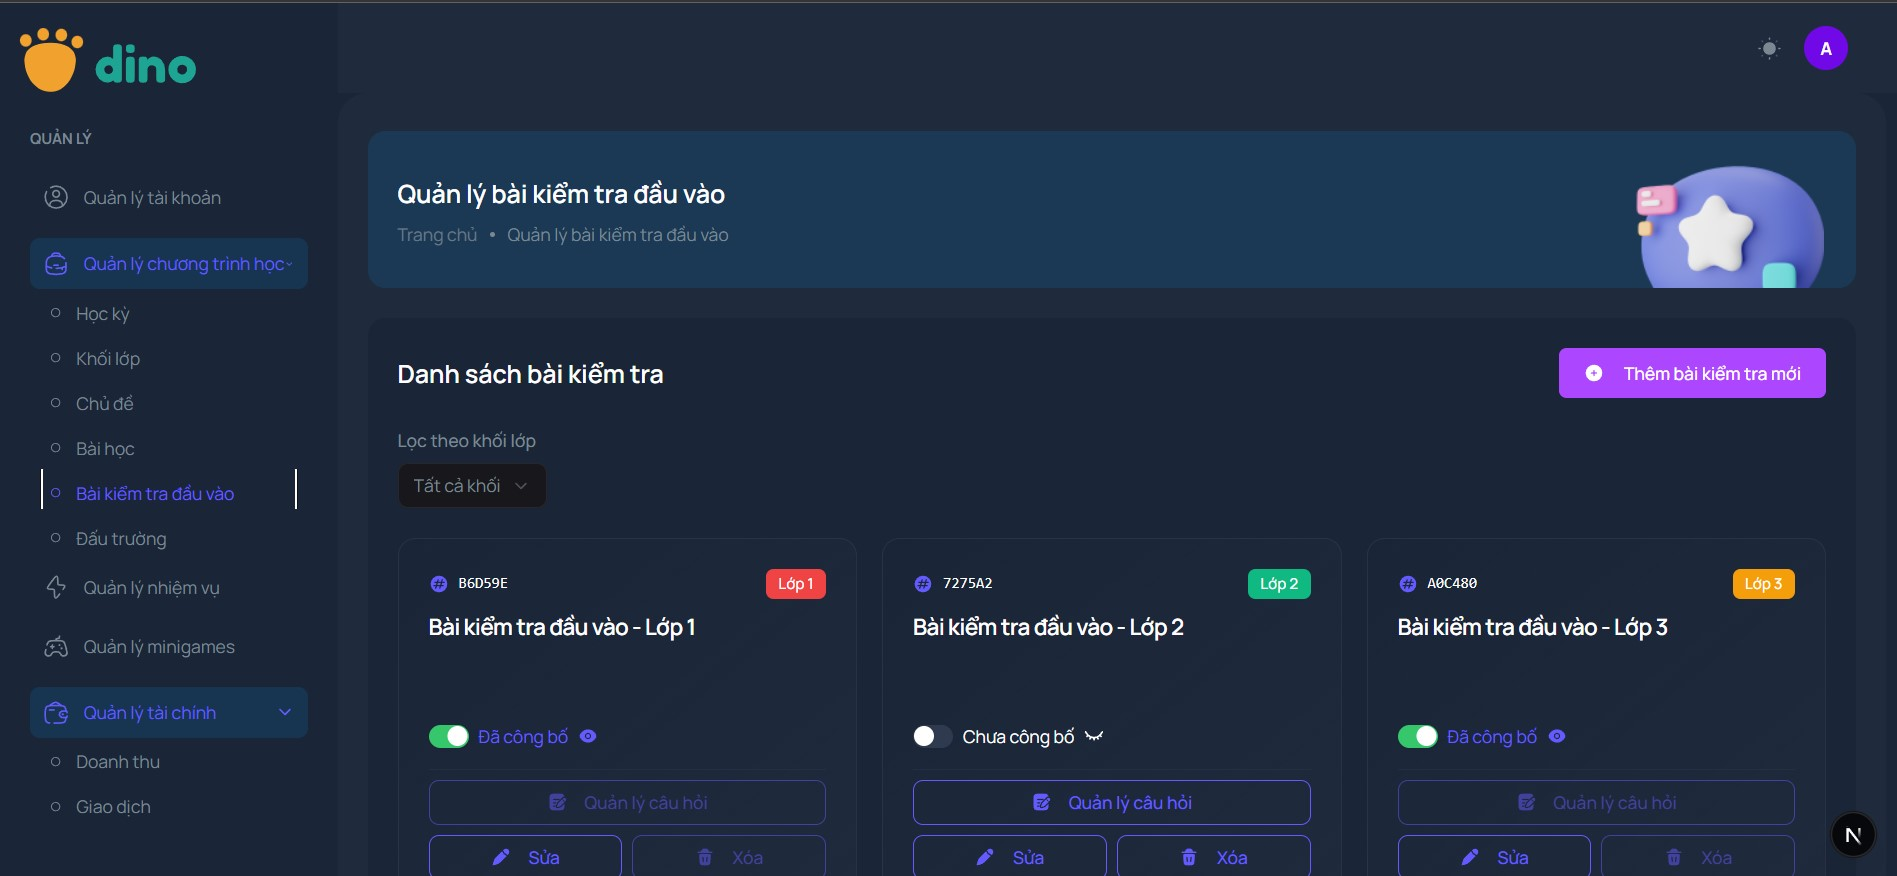
\includegraphics[width=0.9\textwidth]{Image/UI/Admin/Test.jpg}
	\vspace{0.6cm}
	\caption{Admin - Quản lý bài kiểm tra đầu vào}
\end{figure}

\subsubsection{Quản lý đấu trường}
Quản trị viên có thể tạo và quản lý các đấu trường theo tuần. Mỗi đấu trường có thể được lọc theo khối lớp và trạng thái, đồng thời hỗ trợ thiết lập thời gian bắt đầu và kết thúc cụ thể.
\begin{figure}[H]
	\centering
	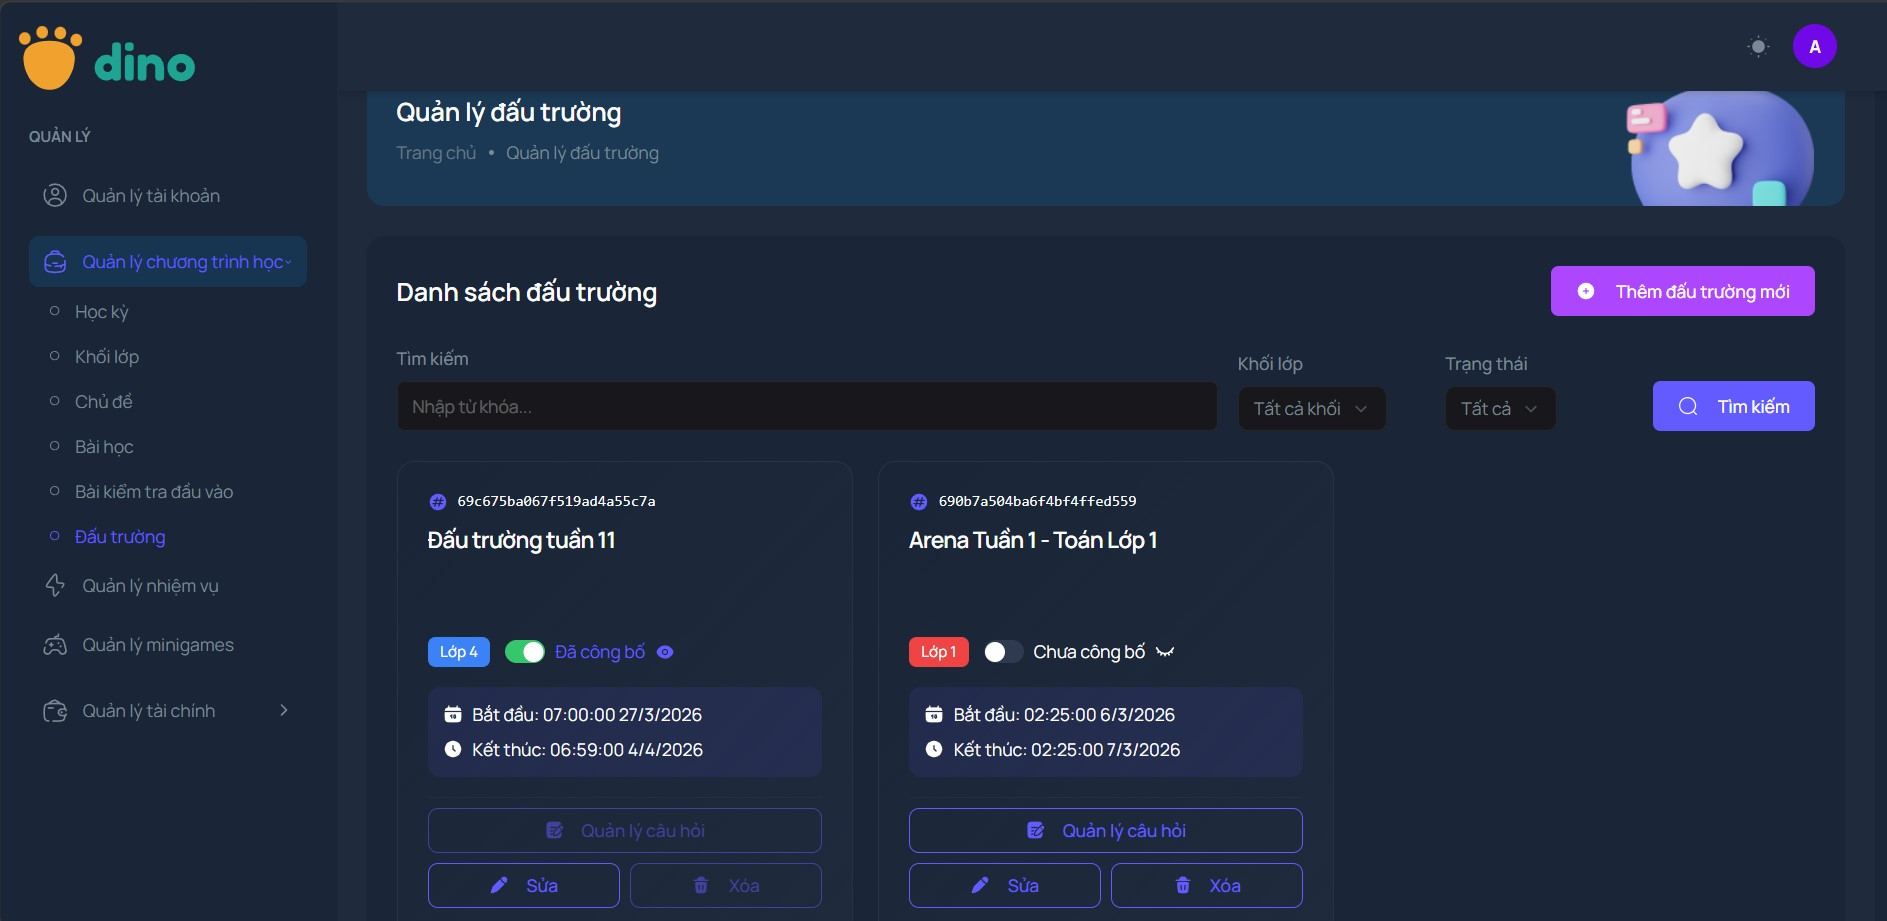
\includegraphics[width=0.9\textwidth]{Image/UI/Admin/Arena.jpg}
	\vspace{0.6cm}
	\caption{Admin - Quản lý đấu trường}
\end{figure}

\subsubsection{Quản lý nhiệm vụ}
Quản trị viên có thể tạo nhiệm vụ hằng ngày, thiết lập điều kiện hoàn thành và phần thưởng tương ứng.
\begin{figure}[H]
	\centering
	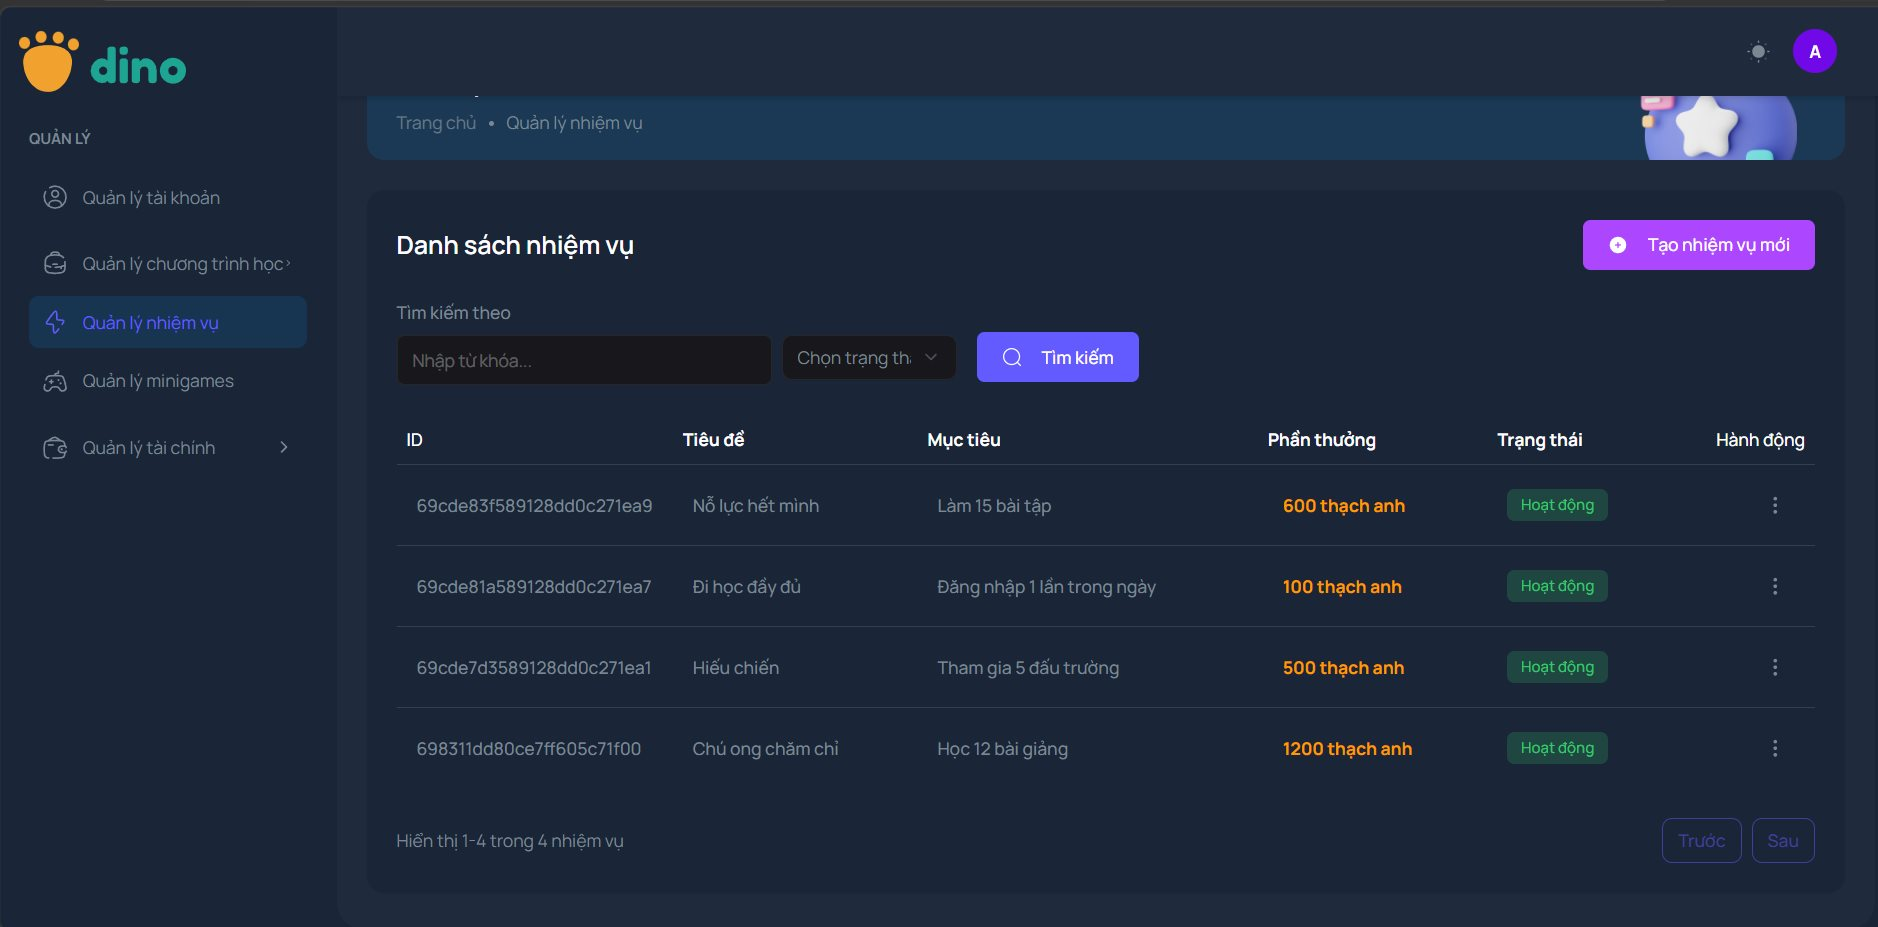
\includegraphics[width=0.9\textwidth]{Image/UI/Admin/Missions.jpg}
	\vspace{0.6cm}
	\caption{Admin - Quản lý nhiệm vụ}
\end{figure}

\subsubsection{Quản lý Minigames}
Quản trị viên có thể tạo và chỉnh sửa nội dung các minigame trong hệ thống.
\begin{figure}[H]
	\centering
	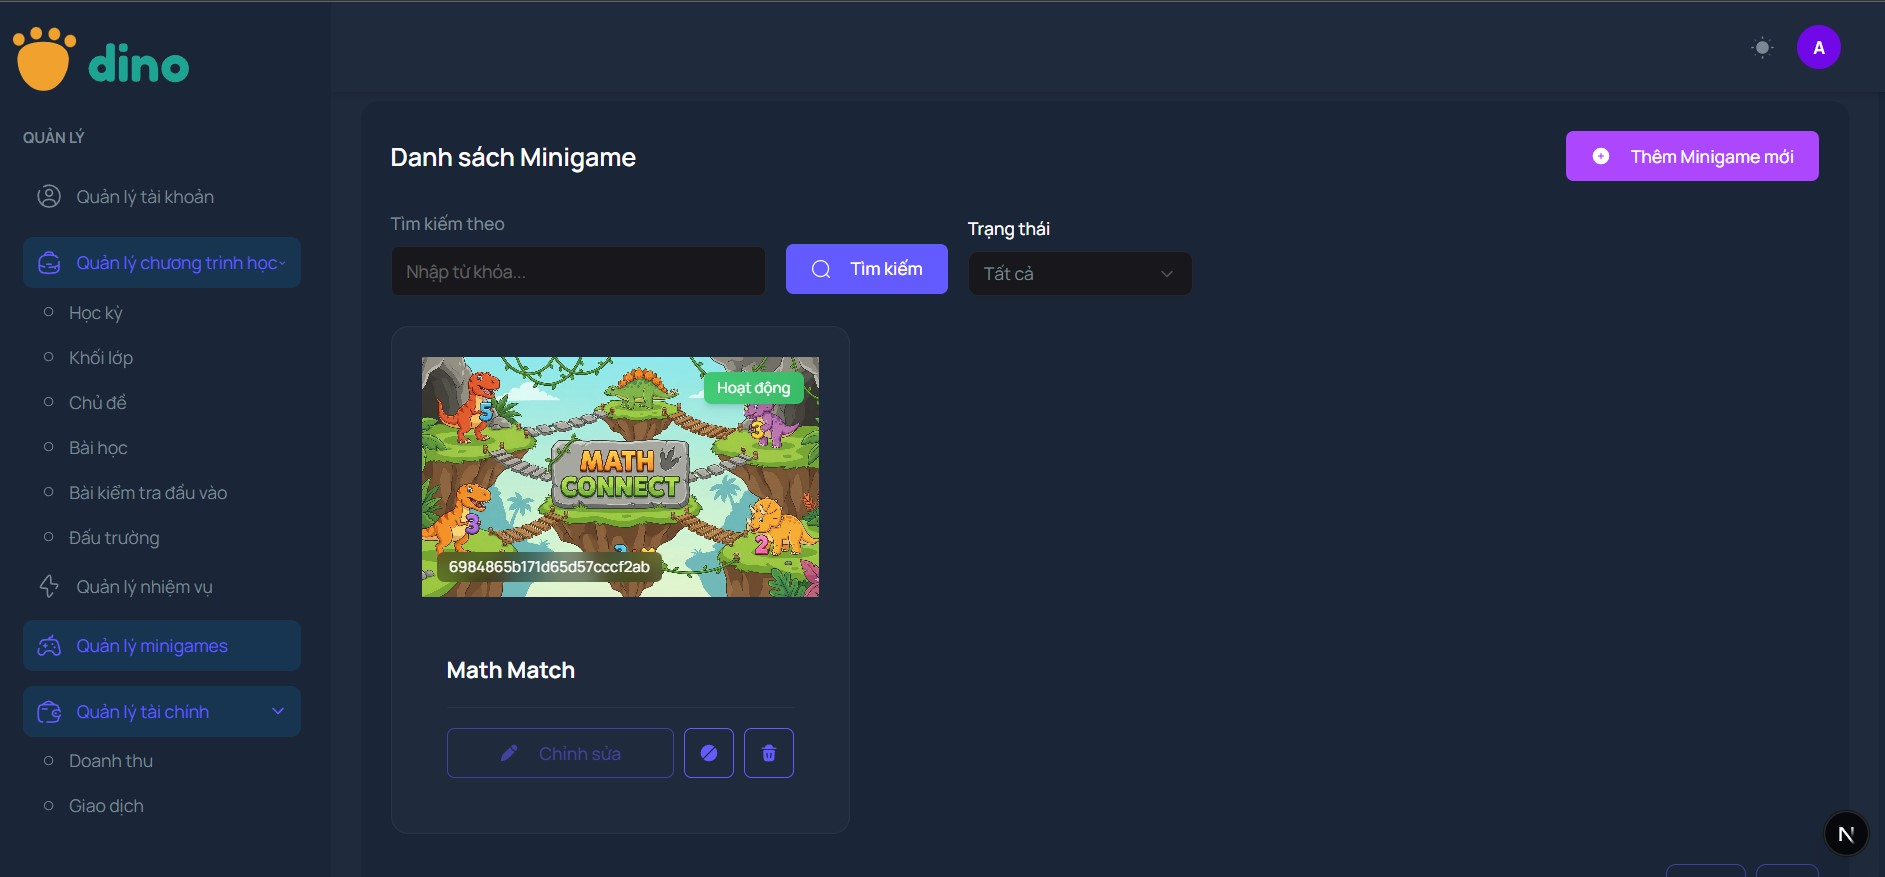
\includegraphics[width=0.9\textwidth]{Image/UI/Admin/Minigame.jpg}
	\vspace{0.6cm}
	\caption{Admin - Quản lý Minigames}
\end{figure}

\subsubsection{Quản lý tài chính}
Quản trị viên có thể xem doanh thu của hệ thống và theo dõi, quản lý các giao dịch thanh toán.
\begin{figure}[H]
	\centering
	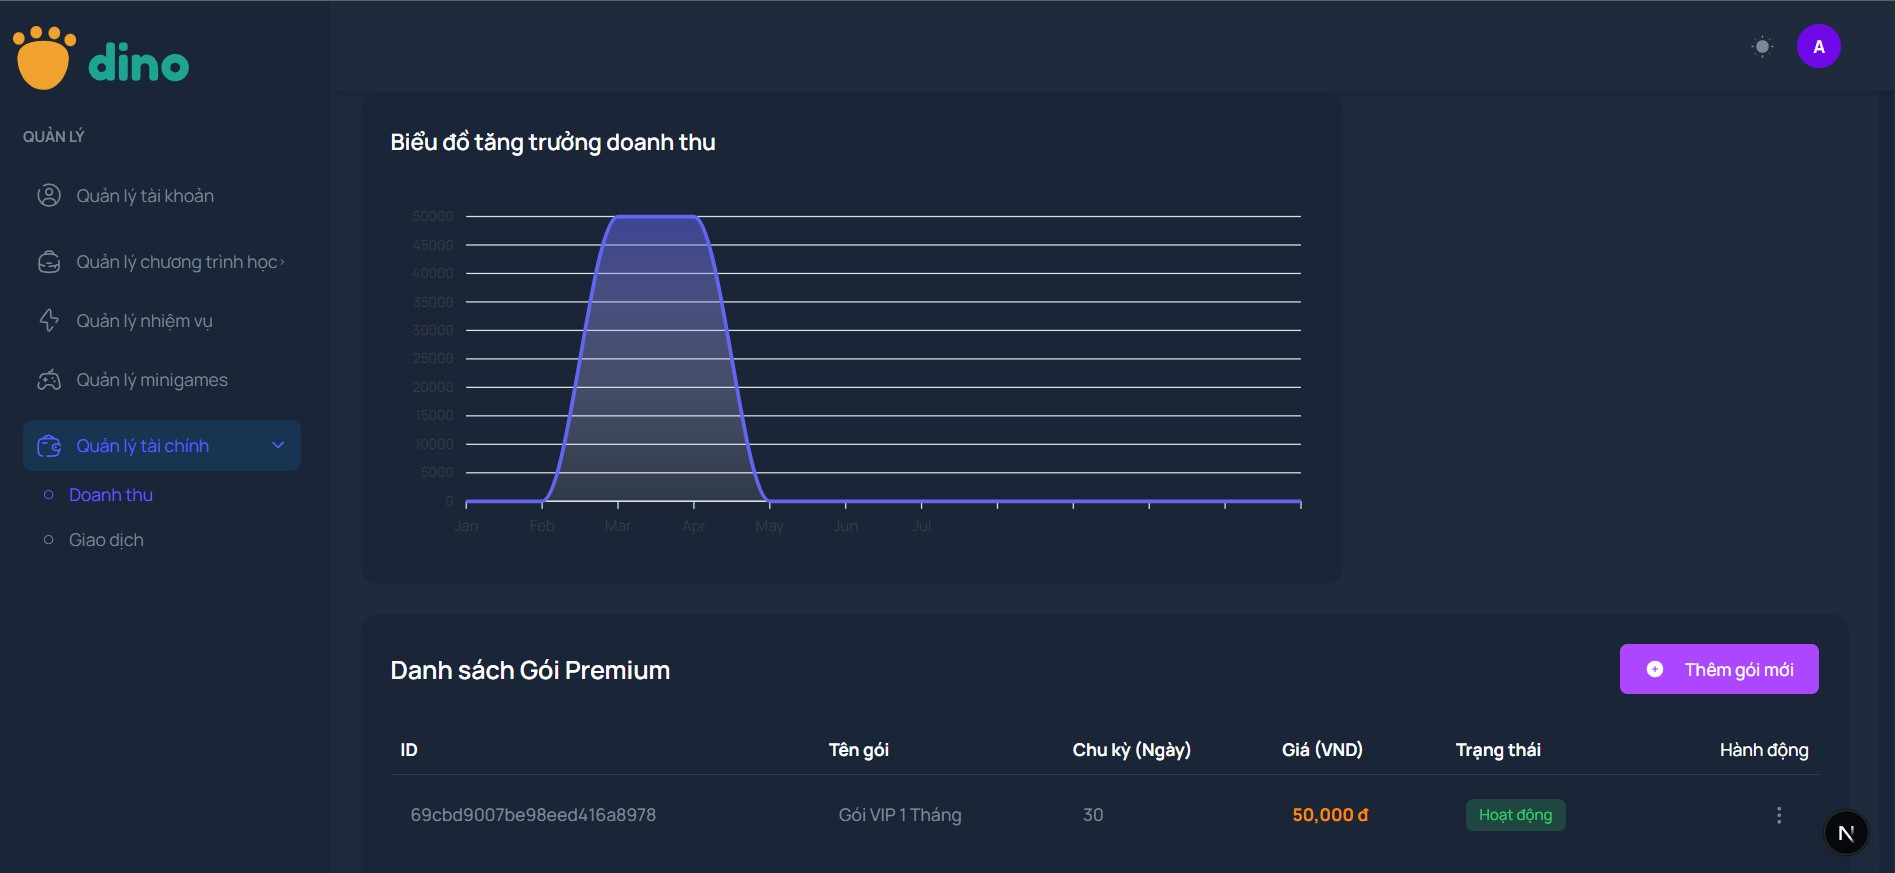
\includegraphics[width=0.9\textwidth]{Image/UI/Admin/Revenue.jpg}
	\vspace{0.6cm}
	\caption{Admin - Quản lý tài chính}
\end{figure}

\subsection{Hệ thống bài tập}
\label{subsec:interact}
Để xây dựng một môi trường học tập toán tư duy hiệu quả, hệ thống bài tập không chỉ dừng lại ở việc kiểm tra kiến thức mà còn phải đóng vai trò là công cụ kích thích sự phát triển trí tuệ. Thiết kế của chúng tôi dựa trên ba trụ cột chính: tính sư phạm, tính tương tác và tính công nghệ.

\subsubsection{Cơ sở thiết kế và chuẩn kiến thức}
Nội dung bài tập được xây dựng dựa trên \textbf{Chương trình Giáo dục phổ thông 2018} của Bộ Giáo dục và Đào tạo Việt Nam \cite{bogddt2018}, tập trung vào 5 mạch kiến thức cốt lõi: Số và phép tính, Hình học và Đo lường, Thống kê và Xác suất. Tuy nhiên, thay vì các bài tập tính toán đơn thuần, chúng tôi tích hợp các phương pháp tư duy từ mô hình giáo dục quốc tế như \textbf{Singapore Math (phương pháp CPA: Concrete-Pictorial-Abstract)} \cite{leong2015concrete} để giúp học sinh Việt Nam dễ dàng chuyển đổi từ tư duy trực quan sang tư duy trừu tượng.

Về mặt học thuật, hệ thống bài tập được tổ chức theo tiến trình phát triển năng lực toán học của học sinh tiểu học từ lớp 1 đến lớp 5, bảo đảm tính kế thừa, đồng tâm và mở rộng dần theo từng khối lớp. Mỗi chủ đề được thiết kế theo ba mức độ \textit{nhận biết -- thông hiểu -- vận dụng}, tương ứng với khả năng nhận diện khái niệm, thực hiện thao tác và giải quyết tình huống thực tiễn; ví dụ từ nhận biết số, phép tính cơ bản ở lớp 1 đến phân số, số thập phân, tỉ số, hình học và toán ứng dụng ở các lớp trên. Cách tổ chức này giúp ngân hàng bài tập vừa bám sát chuẩn đầu ra của chương trình, vừa hỗ trợ hình thành tư duy phân tích, lập luận và giải quyết vấn đề thông qua các ngữ cảnh gần gũi với đời sống học sinh.

\subsubsection{Kiến trúc mô-đun và Công nghệ phát triển}
Hệ thống được thiết kế dựa trên kiến trúc mô-đun linh hoạt, cho phép tách biệt giữa dữ liệu bài toán (Content) và logic tương tác (Logic). 

\begin{itemize}
	\item \textbf{Công cụ phát triển:} Toàn bộ hệ thống tương tác được phát triển trên engine \textbf{Cocos Creator 3.8} \cite{cocoscreator38}. Việc sử dụng hệ thống \textit{Entity Component System (ECS)} của Cocos Creator giúp tối ưu hóa hiệu suất xử lý đồng thời trên cả nền tảng Web và Mobile, đảm bảo các hiệu ứng hoạt hình và phản hồi vật lý mượt mà.
	\item \textbf{Tính mở rộng:} Nhờ vào khả năng quản lý tài nguyên (Asset Management) mạnh mẽ của Cocos 3.8, hệ thống dễ dàng tích hợp thêm các dạng bài tập mới (Drag-and-Drop, Fill-in-the-blank, Logic Matching) mà không làm ảnh hưởng đến cấu trúc tổng thể của ứng dụng.
\end{itemize}

\subsubsection{Giải pháp tương tác và Game hóa (Gamification)}
Khắc phục nhược điểm của các hệ thống cũ tại Việt Nam vốn nặng về lý thuyết, giải pháp của chúng tôi ứng dụng các nguyên lý trong \textbf{Khung lý thuyết Octalysis} \cite{chou2015} để thiết kế hệ thống phần thưởng và nhiệm vụ:
\begin{itemize}
	\item \textbf{Phản hồi tức thì (Instant Feedback):} Sử dụng hệ thống Particle và Animation trong Cocos Creator để tạo ra các hiệu ứng khích lệ khi học sinh giải đúng, giúp duy trì trạng thái "Flow" (luồng hứng thú) trong quá trình học.
	\item \textbf{Tương tác đa chạm:} Tận dụng tối đa bộ lọc sự kiện (Input Events) của Cocos để tạo ra các bài tập kéo thả vật thể, xoay hình học không gian, giúp học sinh tiểu học phát triển tư duy hình khối một cách trực quan nhất.
\end{itemize}

\subsubsection{Các dạng toán}

\subsubsubsection{Trắc nghiệm (Multiple Choice)}
Dạng bài tập trắc nghiệm cho phép người học lựa chọn một đáp án đúng trong bốn đáp án được cung cấp sẵn. Sau khi chọn đáp án, hệ thống sẽ phản hồi trực quan bằng hiệu ứng nhấp nháy hoặc đổi màu để giúp học sinh nhận biết kết quả ngay lập tức. Dạng bài này thường được sử dụng để luyện tập các phép tính cơ bản, nhận diện hình học, so sánh số hoặc các câu hỏi lý thuyết đơn giản phù hợp với học sinh tiểu học.

\begin{figure}[H]
	\centering
	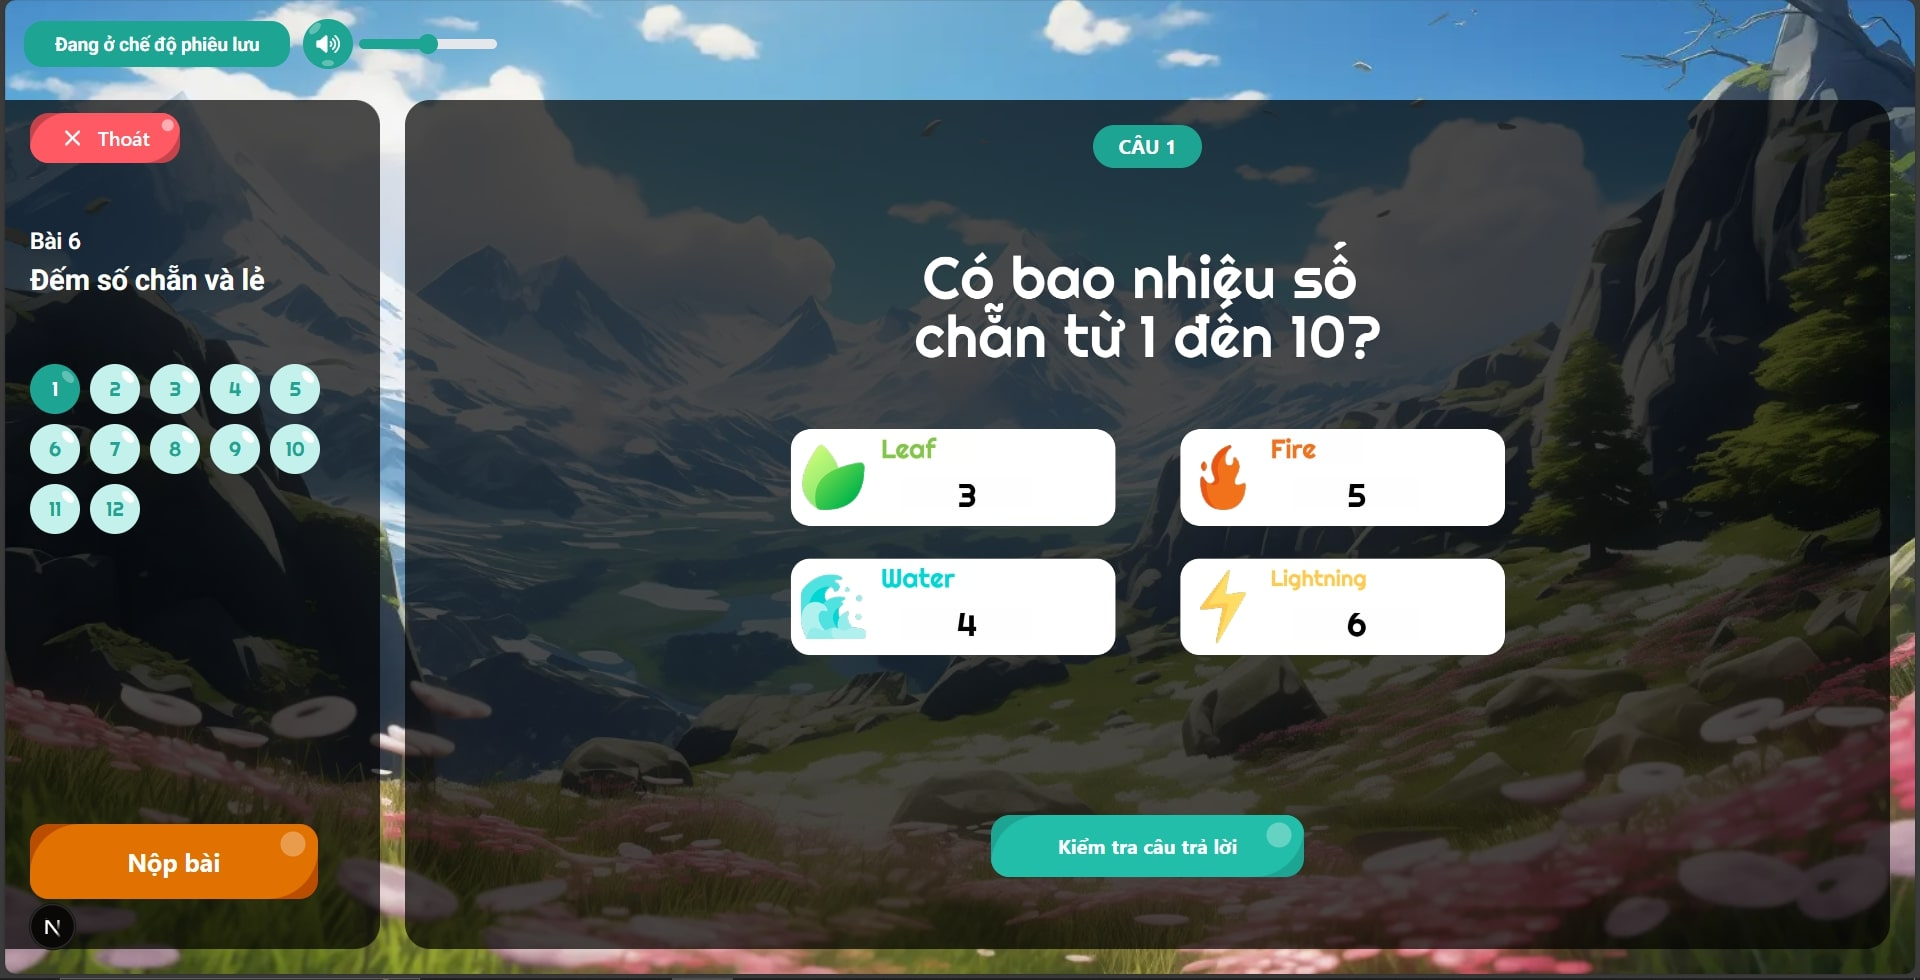
\includegraphics[width=0.9\textwidth]{Image/UI/Exercises/MultiChoice.jpg}
	\caption{Dạng bài trắc nghiệm}
	\label{fig:multiple-choice}
\end{figure}

\subsubsubsection{Ghép cặp (Matching)}
Trong dạng bài ghép cặp, người học thực hiện thao tác kéo thả để nối các đối tượng tương ứng với nhau, ví dụ như phép tính với kết quả tương ứng. Khi ghép đúng, các đối tượng sẽ đổi màu hoặc xuất hiện hiệu ứng phản hồi nhằm tăng tính trực quan và tạo cảm giác hứng thú trong quá trình học tập.

\begin{figure}[H]
	\centeringMô 
	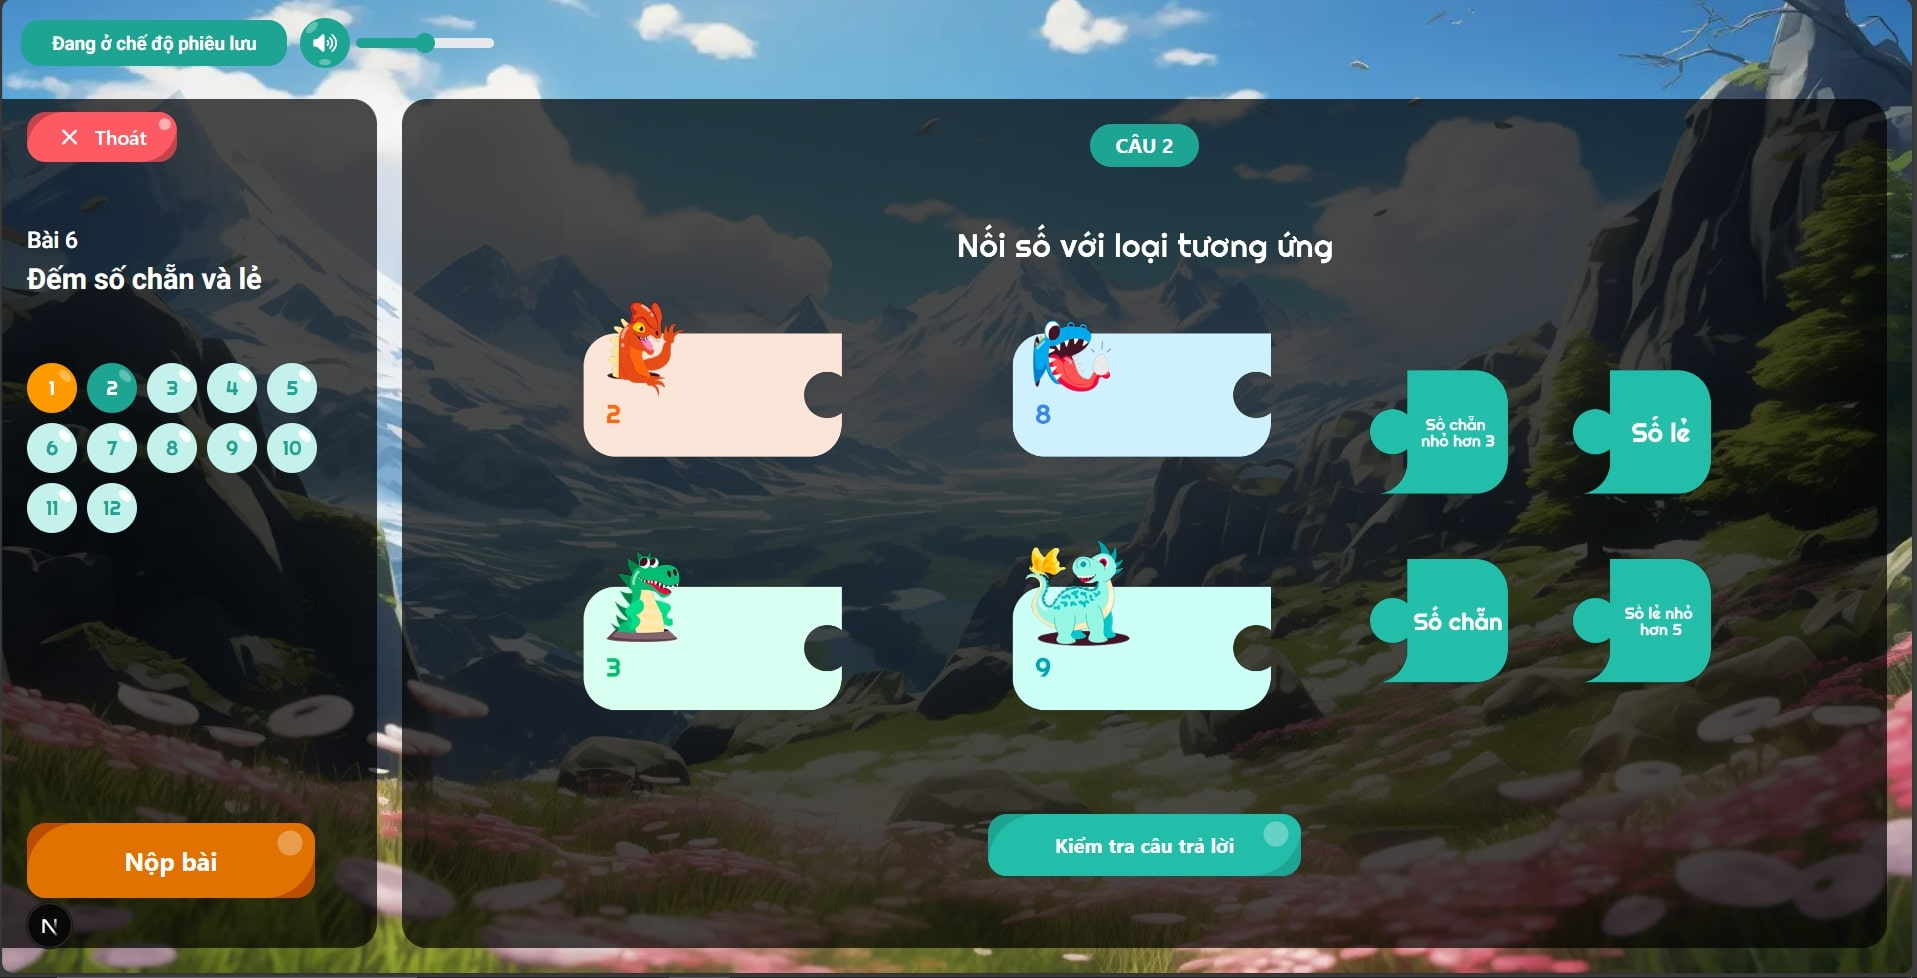
\includegraphics[width=0.9\textwidth]{Image/UI/Exercises/Matching.jpg}
	\caption{Dạng bài ghép cặp}
	\label{fig:matching}
\end{figure}

\subsubsubsection{Điền số (Fill in the Blanks)}
Dạng bài điền số yêu cầu học sinh nhập giá trị thích hợp vào các ô trống trong biểu thức hoặc câu hỏi toán học. Một bài có thể chứa tối đa ba ô trống và hệ thống sẽ chấm điểm độc lập cho từng phần nhằm hỗ trợ đánh giá chính xác hơn. Dạng bài này giúp rèn luyện khả năng tính toán và tư duy từng bước của người học.

\begin{figure}[H]
	\centering
	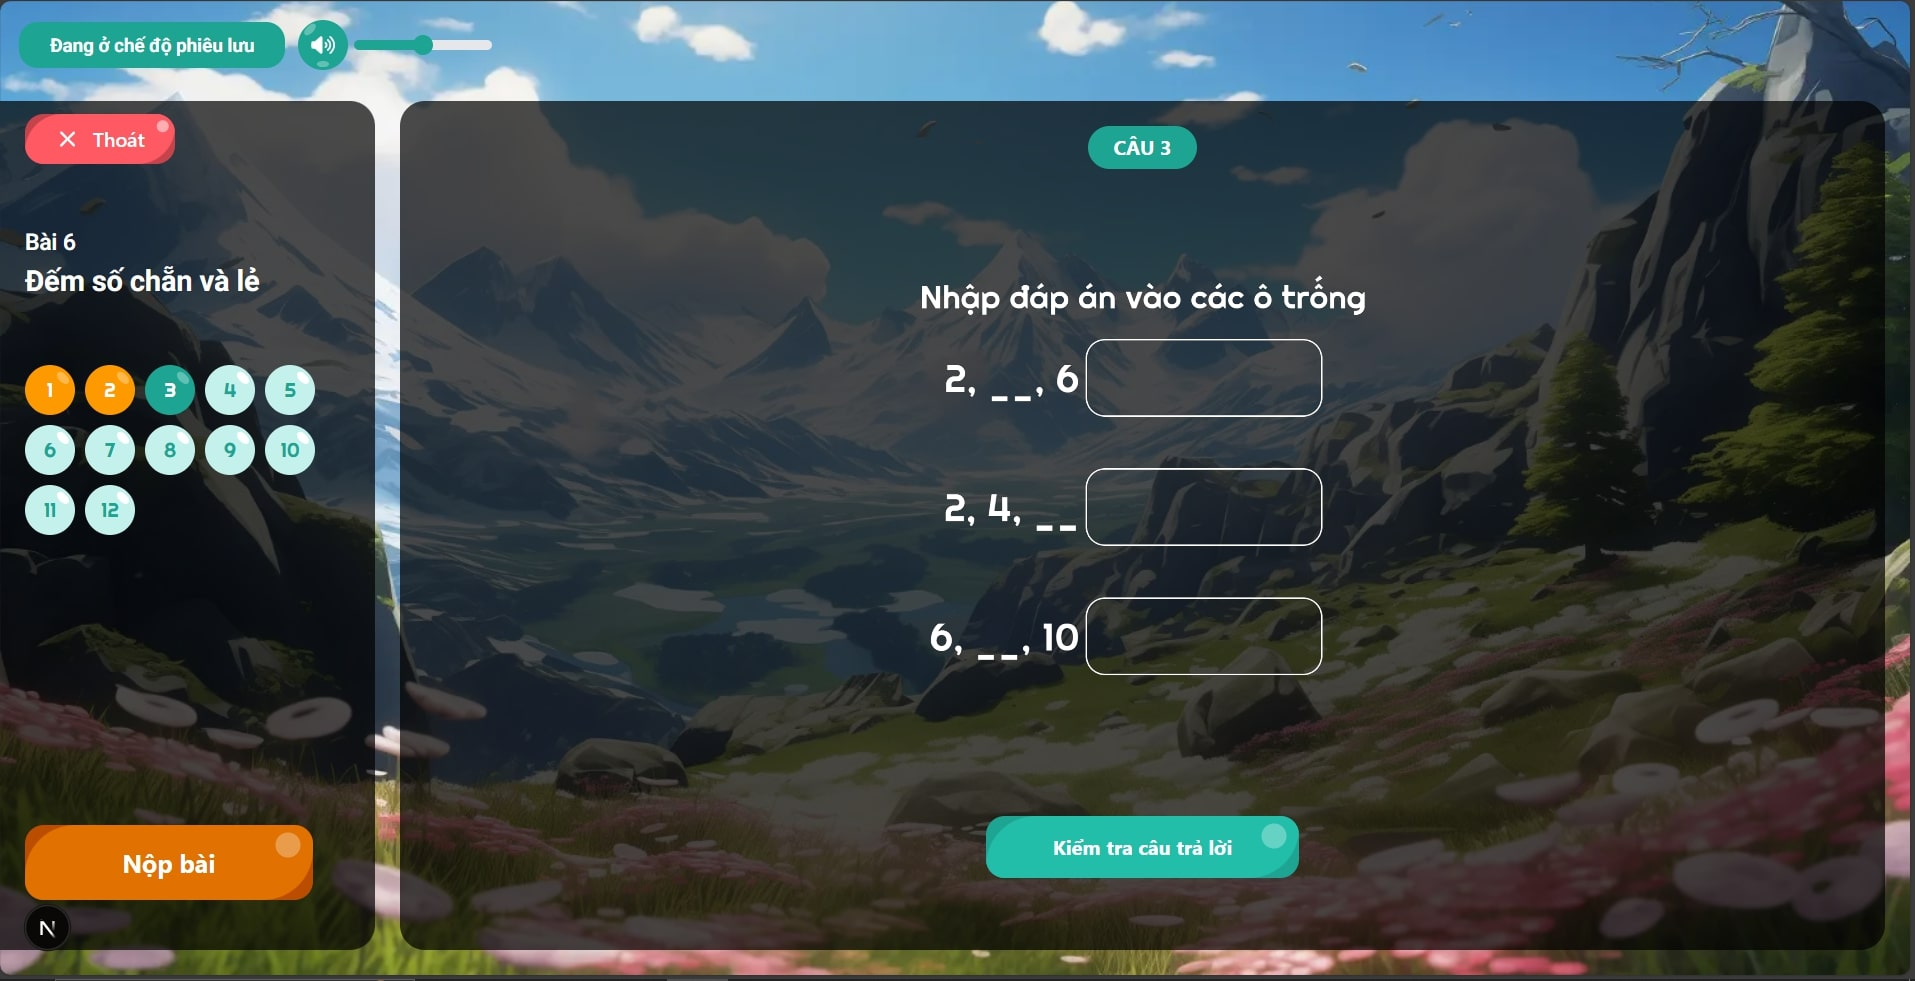
\includegraphics[width=0.9\textwidth]{Image/UI/Exercises/Fill.jpg}
	\caption{Dạng bài điền số}
	\label{fig:fill}
\end{figure}

\subsubsubsection{Kéo thả (Drag and Drop)}
Ở dạng bài này, người học sẽ kéo các con số hoặc ký hiệu toán học vào đúng vị trí còn thiếu trong biểu thức. Nếu thả sai vị trí, hệ thống sẽ tự động đưa đối tượng trở về vị trí ban đầu để người học thử lại. Cơ chế tương tác trực tiếp giúp học sinh dễ dàng tiếp cận và ghi nhớ các phép tính cơ bản.

\begin{figure}[H]
	\centering
	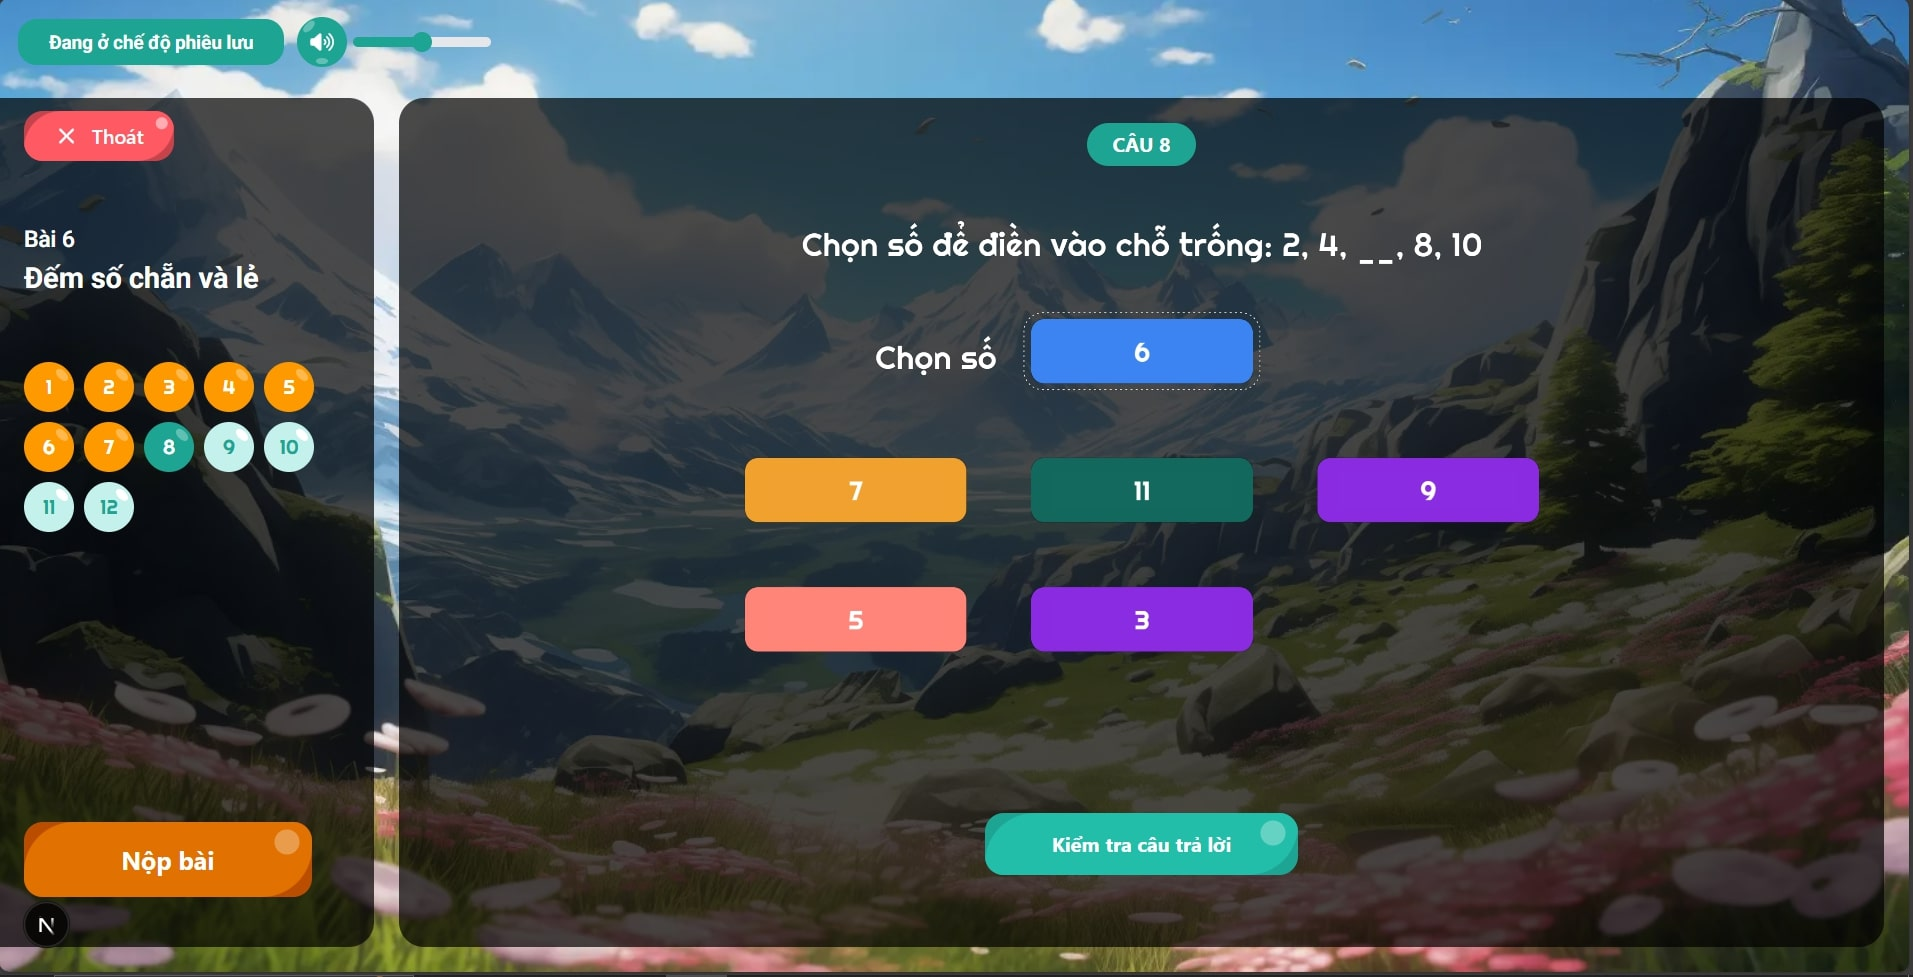
\includegraphics[width=0.9\textwidth]{Image/UI/Exercises/Drag.jpg}
	\caption{Dạng bài kéo thả}
	\label{fig:drag}
\end{figure}

\subsubsubsection{Phân loại chẵn/lẻ (Grouping)}
Dạng bài phân loại yêu cầu học sinh lựa chọn chế độ phân loại trước khi bắt đầu làm bài, trong đó số chẵn được biểu diễn bằng màu xanh và số lẻ được biểu diễn bằng màu hồng. Sau khi chọn chế độ, người học sẽ click trực tiếp vào từng con số để tô màu tương ứng, tương tự như một trò chơi tô màu tương tác. Hệ thống chỉ kiểm tra kết quả sau khi hoàn thành toàn bộ thao tác, giúp học sinh tập trung vào quá trình quan sát, suy luận và tự đánh giá trước khi nộp đáp án.

\begin{figure}[H]
	\centering
	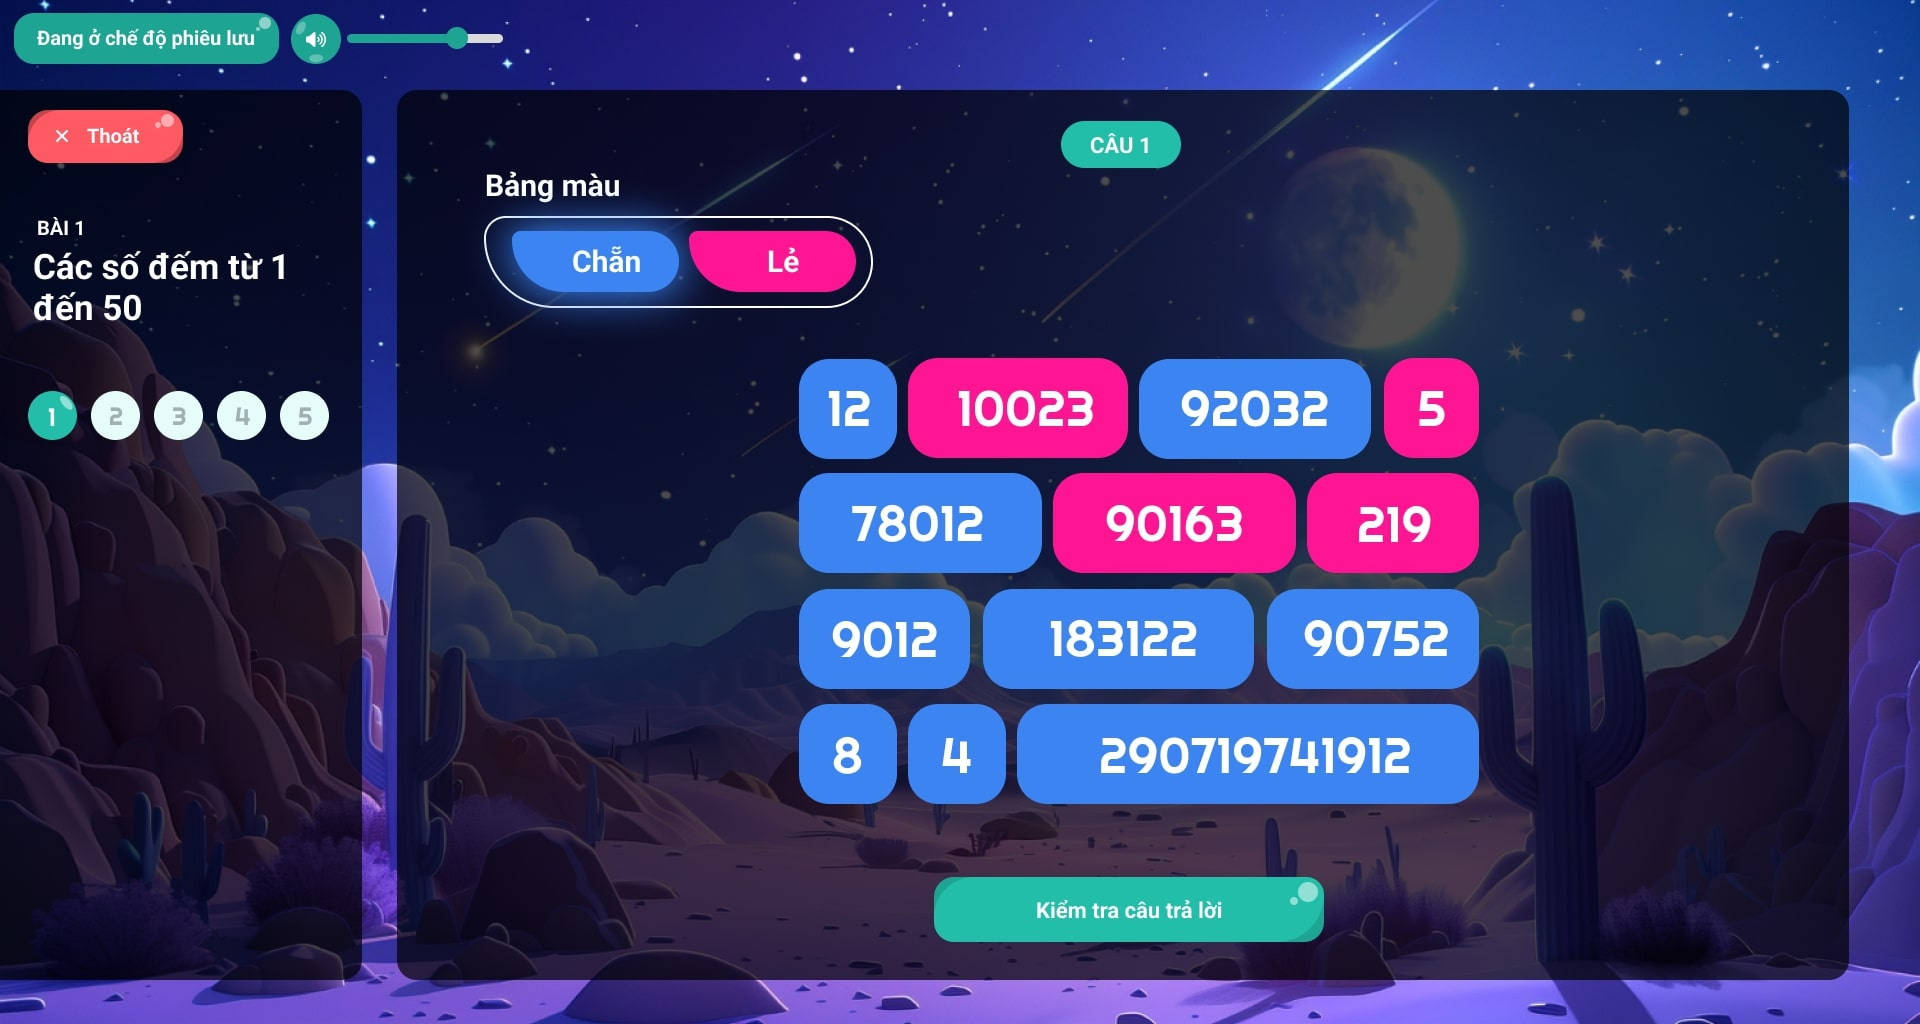
\includegraphics[width=0.9\textwidth]{Image/UI/Exercises/Grouping.jpg}
	\caption{Dạng bài phân loại}
	\label{fig:grouping}
\end{figure}

\subsubsubsection{Đúng/Sai (True/False)}
Dạng bài đúng/sai cung cấp cho người học một mệnh đề hoặc phép tính và yêu cầu lựa chọn “Đúng” hoặc “Sai”. Hệ thống chỉ cho phép một lựa chọn duy nhất nhằm đảm bảo tính rõ ràng trong câu trả lời. Đây là dạng bài đơn giản nhưng hiệu quả trong việc kiểm tra khả năng nhận biết nhanh và tư duy logic của học sinh.

\begin{figure}[H]
	\centering
	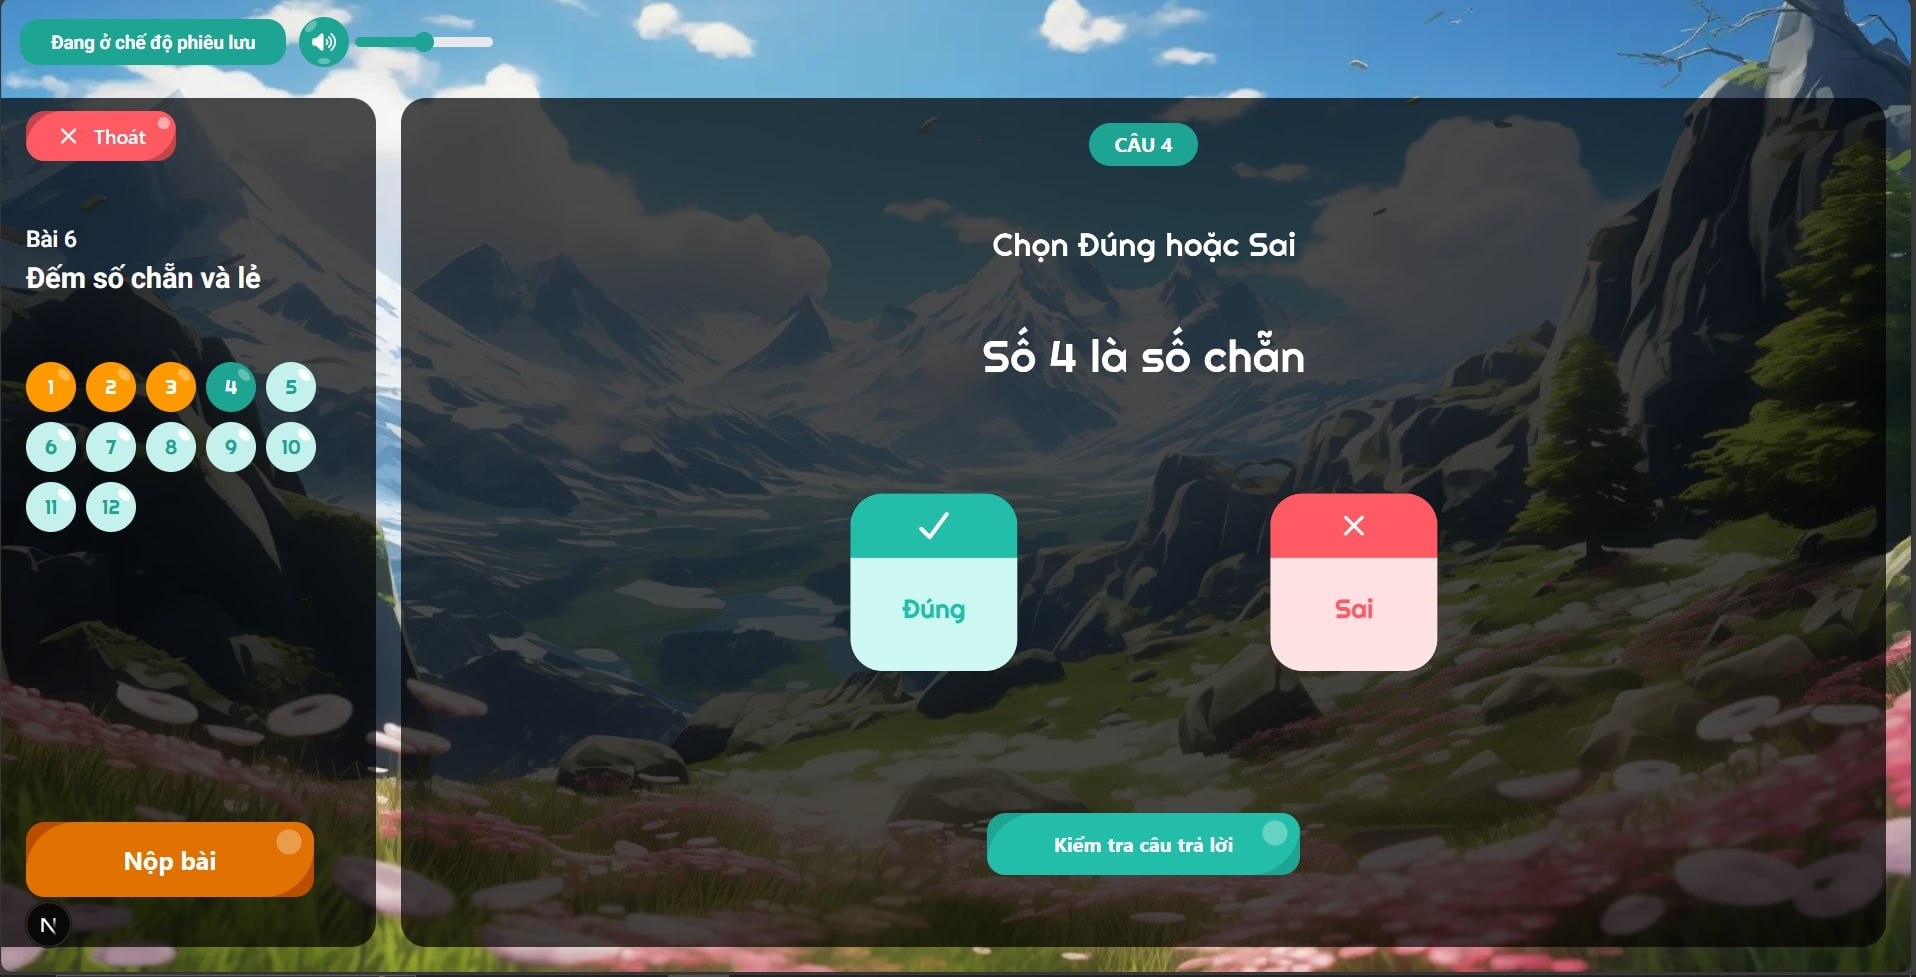
\includegraphics[width=0.9\textwidth]{Image/UI/Exercises/TrueFalse.jpg}
	\caption{Dạng bài đúng/sai}
	\label{fig:truefalse}
\end{figure}

\subsubsubsection{Tổ hợp burger (Burger)}
Dạng bài tổ hợp burger giúp học sinh làm quen với tư duy tổ hợp và lựa chọn thành phần theo yêu cầu đề bài. Hệ thống cung cấp bốn loại nguyên liệu gồm cà chua, thịt, phô mai và rau. Dựa trên yêu cầu của bài toán, người học cần lựa chọn và sắp xếp đúng các nguyên liệu để tạo ra chiếc burger phù hợp. Một bài toán có thể có nhiều cách tạo burger khác nhau miễn đáp ứng đúng yêu cầu về thành phần.

\begin{figure}[H]
	\centering
	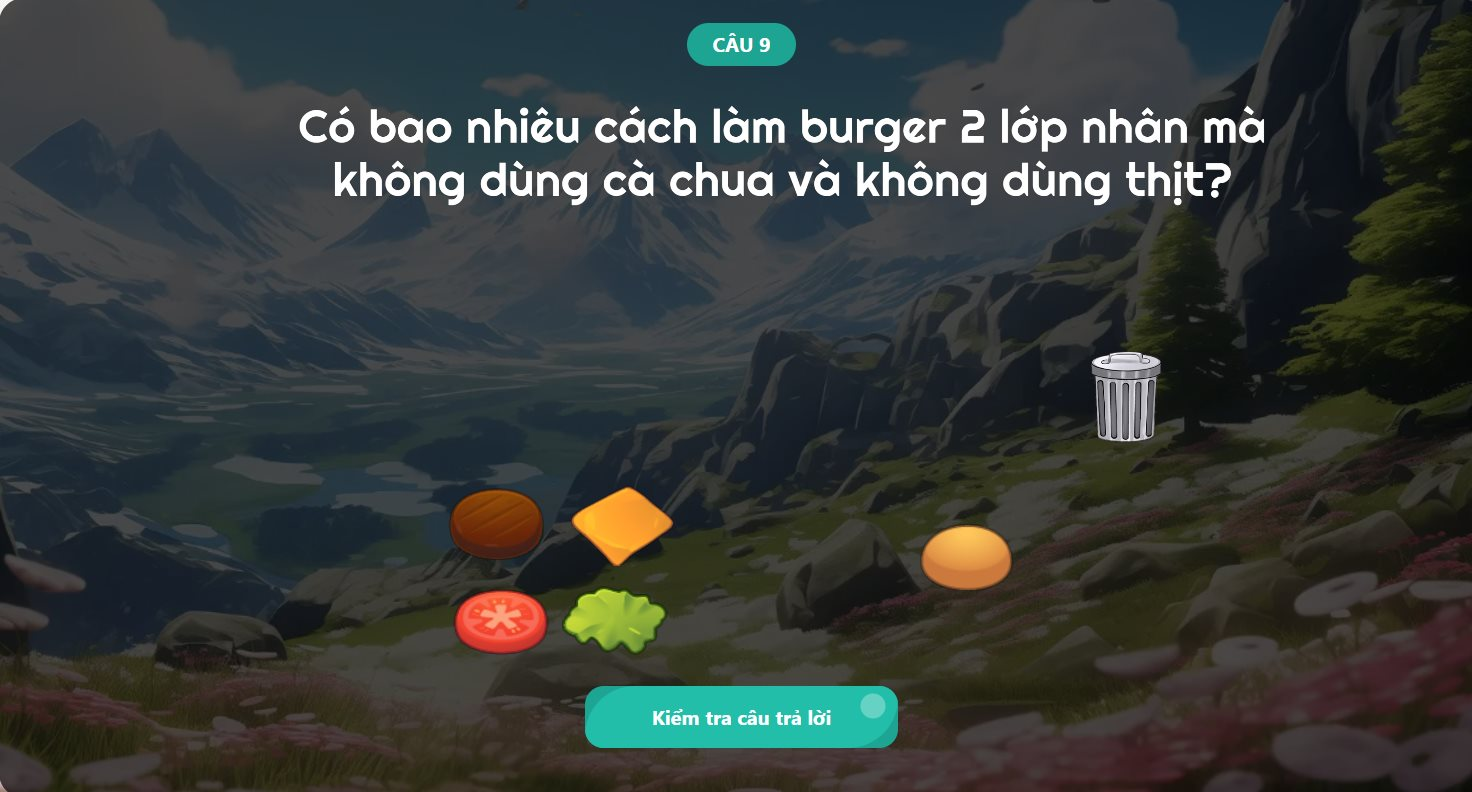
\includegraphics[width=0.9\textwidth]{Image/UI/Exercises/Burger.jpg}
	\caption{Dạng bài tổ hợp burger}
	\label{fig:burger}
\end{figure}

\subsubsubsection{Xe buýt (Bus)}
Dạng bài xe buýt được xây dựng nhằm giúp học sinh hiểu rõ giá trị hàng đơn vị, hàng chục và hàng trăm. Hệ thống cung cấp ba loại hộp tương ứng với giá trị 1, 10 và 100. Theo yêu cầu bài toán, học sinh cần lựa chọn các hộp sao cho tổng giá trị đúng với số lượng cần vận chuyển. Ví dụ, để vận chuyển 100 linh kiện, học sinh có thể chọn một hộp 100 hoặc mười hộp 10. Khi chọn hộp, các hộp sẽ bay trực tiếp lên xe buýt tạo nên trải nghiệm học tập sinh động và trực quan.

\begin{figure}[H]
	\centering
	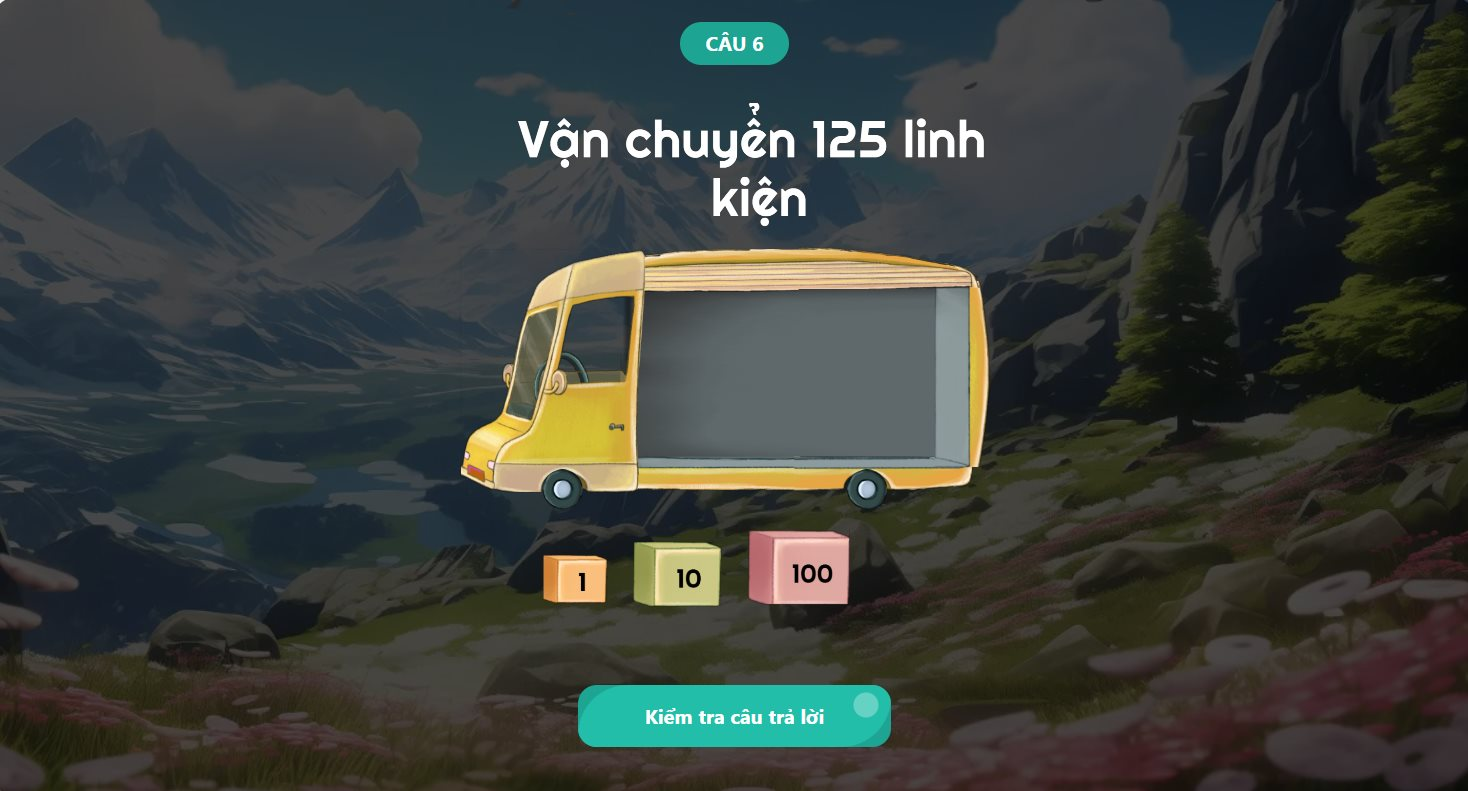
\includegraphics[width=0.9\textwidth]{Image/UI/Exercises/Bus.jpg}
	\caption{Dạng bài xe buýt}
	\label{fig:bus}
\end{figure}

\subsubsubsection{Bắt chim (Catch Bird)}
Trong dạng bài bắt chim, trên cây sẽ có một số lượng chim ban đầu và người học cần click vào các chú chim để chúng bay vào lồng. Số lượng chim trong lồng sẽ đại diện cho kết quả của bài toán. Nhờ cơ chế biểu diễn trực quan này, hệ thống có thể mở rộng thành nhiều dạng câu hỏi khác nhau.

\begin{figure}[H]
	\centering
	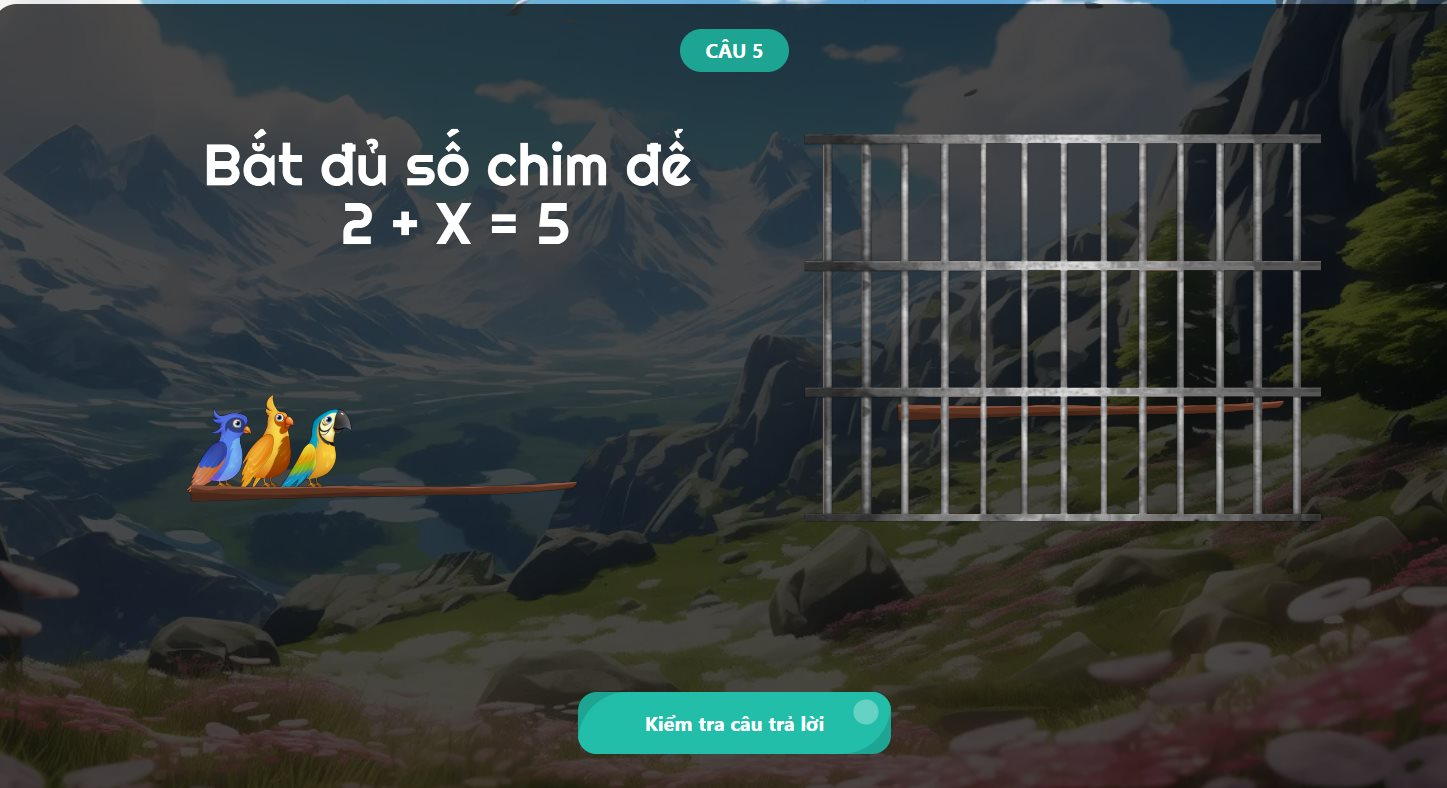
\includegraphics[width=0.9\textwidth]{Image/UI/Exercises/CatchBird.jpg}
	\caption{Dạng bài bắt chim}
	\label{fig:catchbird}
\end{figure}

\subsubsubsection{Đồng hồ (Clock)}
Dạng bài đồng hồ giúp học sinh học cách xem giờ thông qua đồng hồ kim 12 giờ. Người học cần xoay kim đồng hồ đến đúng thời gian được yêu cầu. Điểm đặc biệt của dạng bài này là hệ thống có thêm khung cửa sổ mô phỏng thời gian ngày và đêm. Ví dụ, khi chỉnh đến 12 giờ trưa, khung cửa sổ sẽ hiển thị mặt trời và bầu trời sáng; ngược lại khi chỉnh đến 12 giờ đêm, cửa sổ sẽ hiển thị bầu trời tối cùng mặt trăng. Điều này giúp học sinh phân biệt rõ khái niệm hệ thống giờ 12 giờ và 24 giờ một cách trực quan và sinh động hơn

\begin{figure}[H]
	\centering
	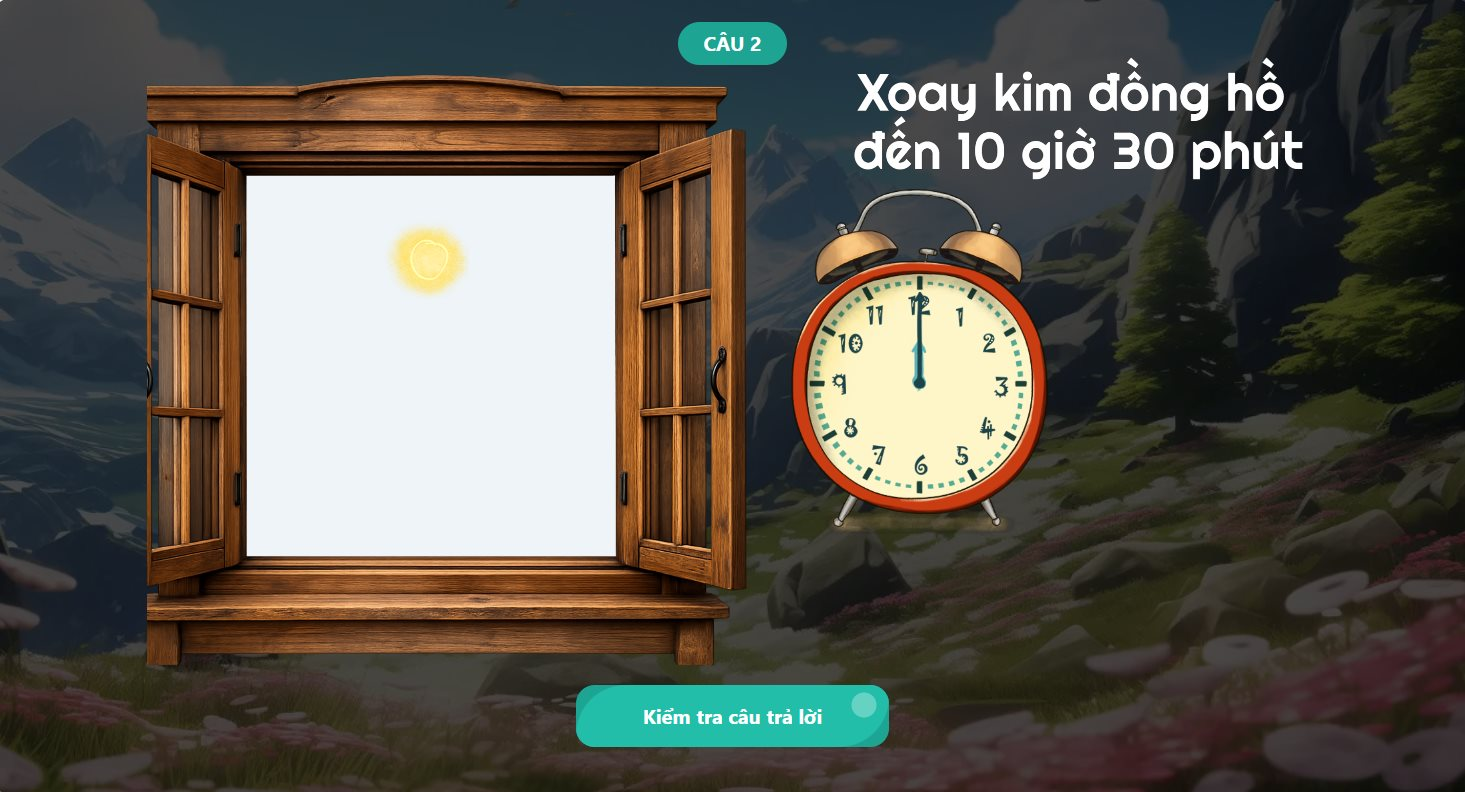
\includegraphics[width=0.9\textwidth]{Image/UI/Exercises/Clock.jpg}
	\caption{Dạng bài đồng hồ}
	\label{fig:clock}
\end{figure}

\subsubsubsection{Đổi tiền xu (Coin)}
Dạng bài đổi tiền xu hỗ trợ học sinh làm quen với giá trị tiền tệ thông qua cơ chế đổi tiền trực quan. Hệ thống cung cấp ba loại đồng xu có giá trị 1 đồng, 10 đồng và 100 đồng cùng với một máy đổi tiền. Khi đưa một đồng xu vào máy, hệ thống sẽ tự động đổi sang các đồng xu có giá trị nhỏ hơn, ví dụ một đồng 100 sẽ đổi thành mười đồng 10. Người học cần vận dụng cơ chế đổi tiền để tạo đúng số tiền theo yêu cầu của bài toán.

\begin{figure}[H]
	\centering
	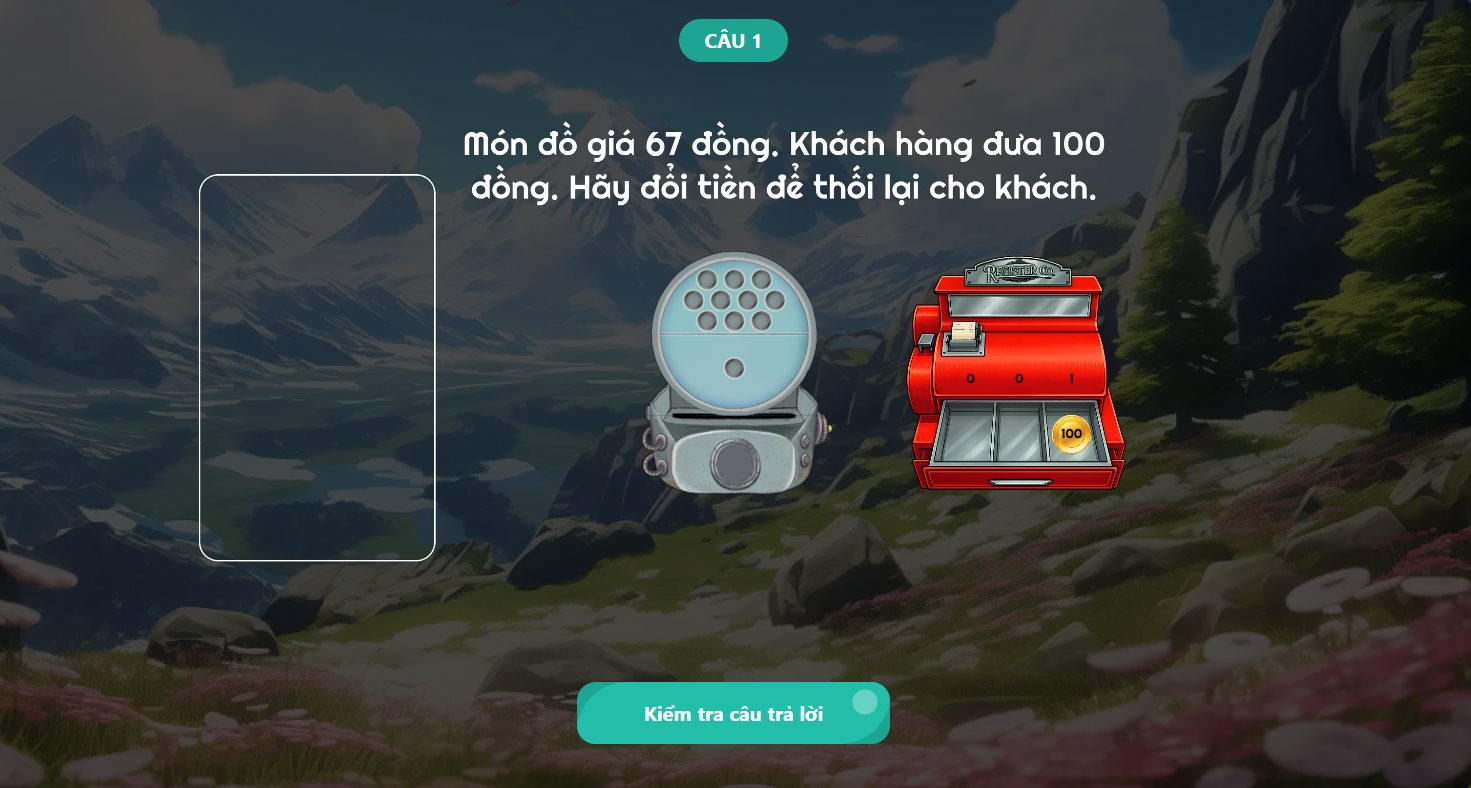
\includegraphics[width=0.9\textwidth]{Image/UI/Exercises/Coin.jpg}
	\caption{Dạng bài đổi tiền xu}
	\label{fig:coin}
\end{figure}

\subsubsubsection{Viên bi (Gumball)}
Dạng bài viên bi được thiết kế nhằm hỗ trợ học sinh luyện tập kỹ năng đếm và so sánh số lượng. Ban đầu hệ thống cung cấp một số lượng bi xanh và bi cam nhất định. Khi người học chọn một chiếc lọ, chiếc lọ sẽ di chuyển vào máy để hứng bi rơi xuống. Mỗi lần máy sẽ thả 10 viên bi và mỗi lọ chứa đúng 10 viên. Học sinh cần quan sát số lọ đã đầy cùng số viên còn lại để trả lời các câu hỏi so sánh như màu nào nhiều hơn hoặc ít hơn.

\begin{figure}[H]
	\centering
	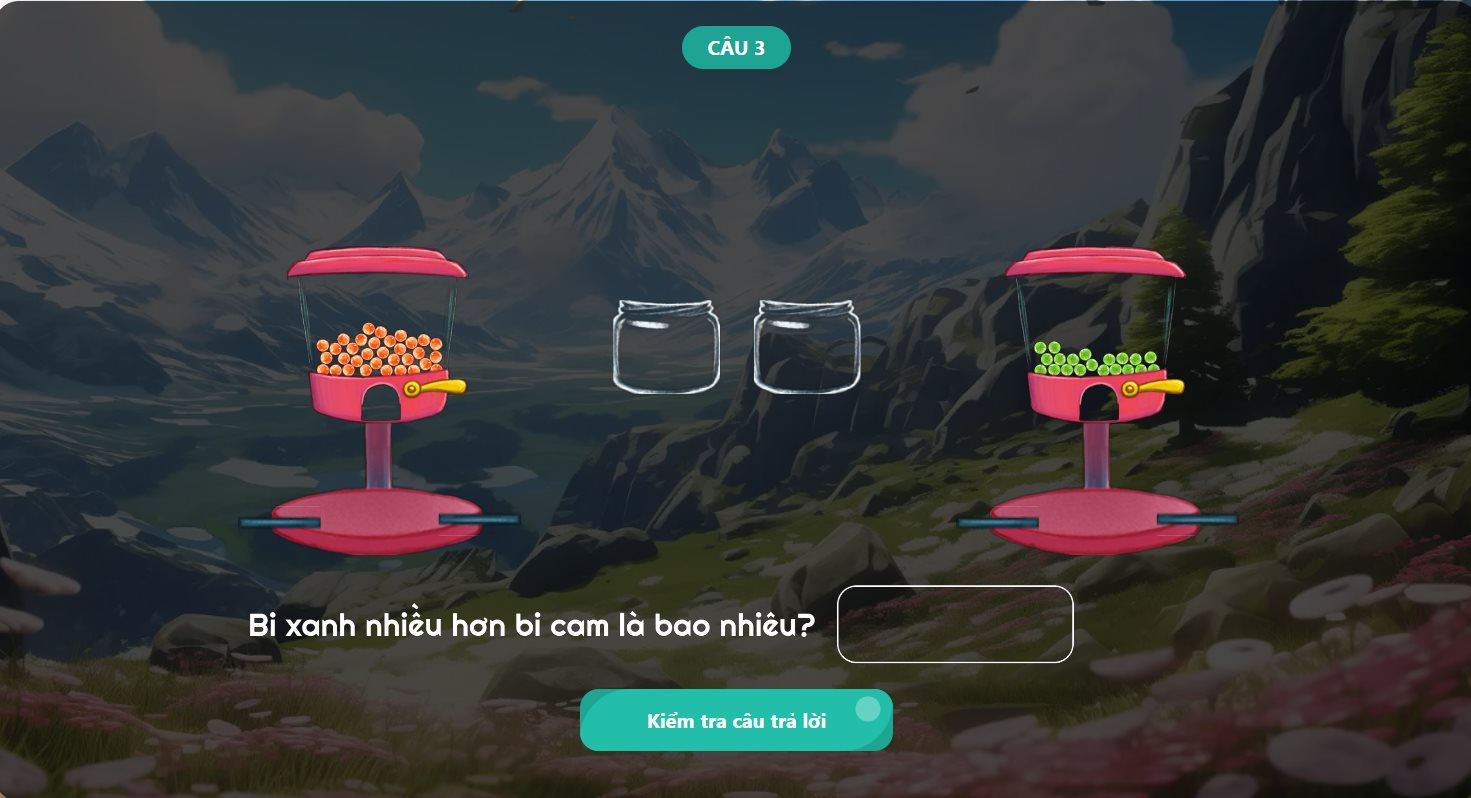
\includegraphics[width=0.9\textwidth]{Image/UI/Exercises/Gumball.jpg}
	\caption{Dạng bài viên bi}
	\label{fig:gumball}
\end{figure}

\subsubsubsection{Cân thủ công (Manual Scale)}
Dạng bài cân thủ công sử dụng mô hình cân đòn nhằm giúp học sinh làm quen với các khái niệm lớn hơn, bé hơn và bằng nhau. Người học sẽ kéo các bát hạt lên hai bên cân theo yêu cầu của đề bài. Dựa vào độ nghiêng của cân sang trái hoặc phải, học sinh có thể trực quan nhận biết mối quan hệ giữa hai giá trị.

\begin{figure}[H]
	\centering
	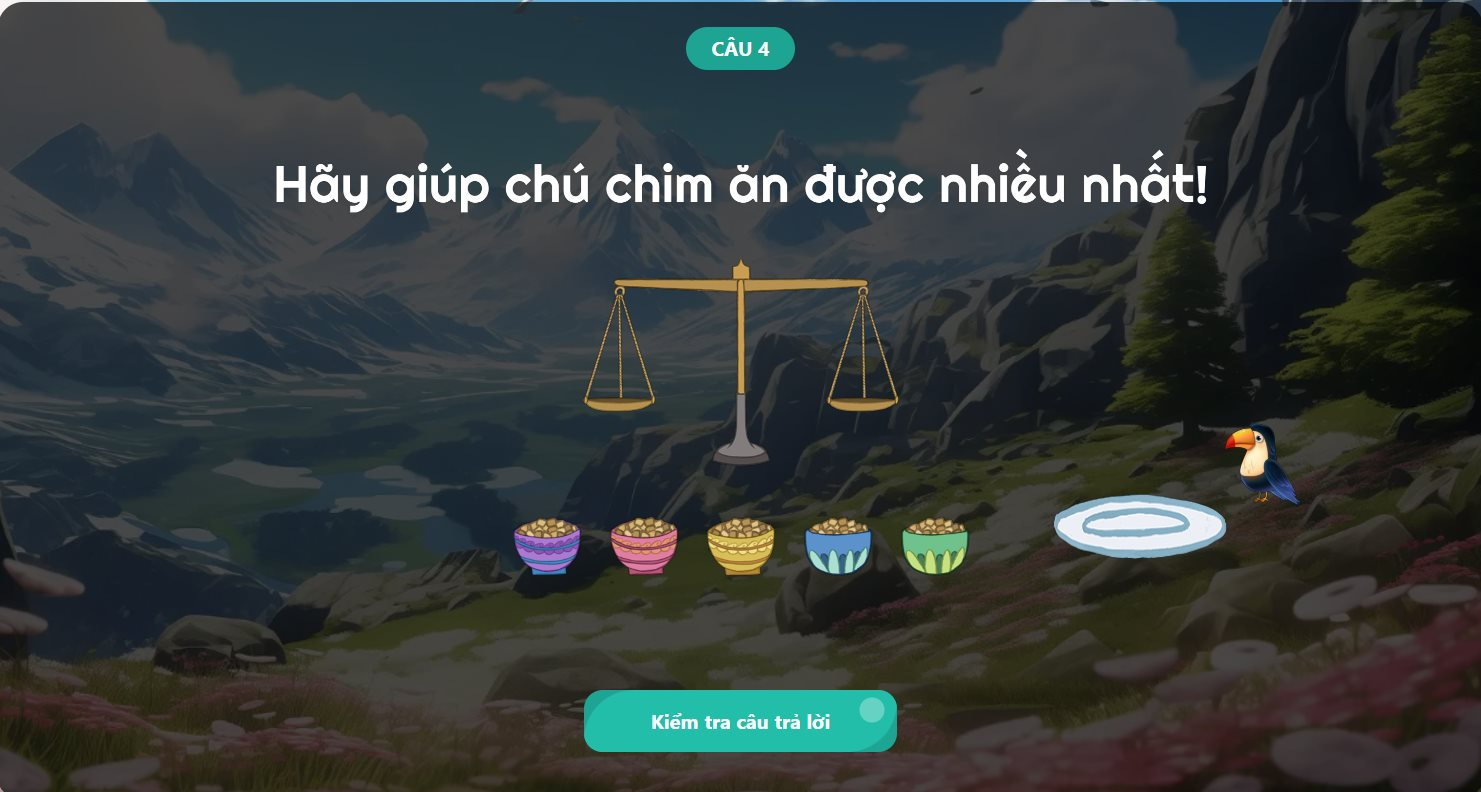
\includegraphics[width=0.9\textwidth]{Image/UI/Exercises/ManualScale.jpg}
	\caption{Dạng bài cân thủ công}
	\label{fig:manual-scale}
\end{figure}

\subsubsubsection{Chia pizza (Pizza)}
Dạng bài chia pizza giúp học sinh bước đầu làm quen với phân số thông qua việc chia chiếc pizza thành nhiều phần bằng nhau. Mỗi lát pizza sẽ có một loại topping khác nhau và bài toán sẽ yêu cầu người học tạo đúng số lượng lát tương ứng với từng loại. Dạng bài này giúp học sinh hình dung trực quan khái niệm phân số trong toán học.

\begin{figure}[H]
	\centering
	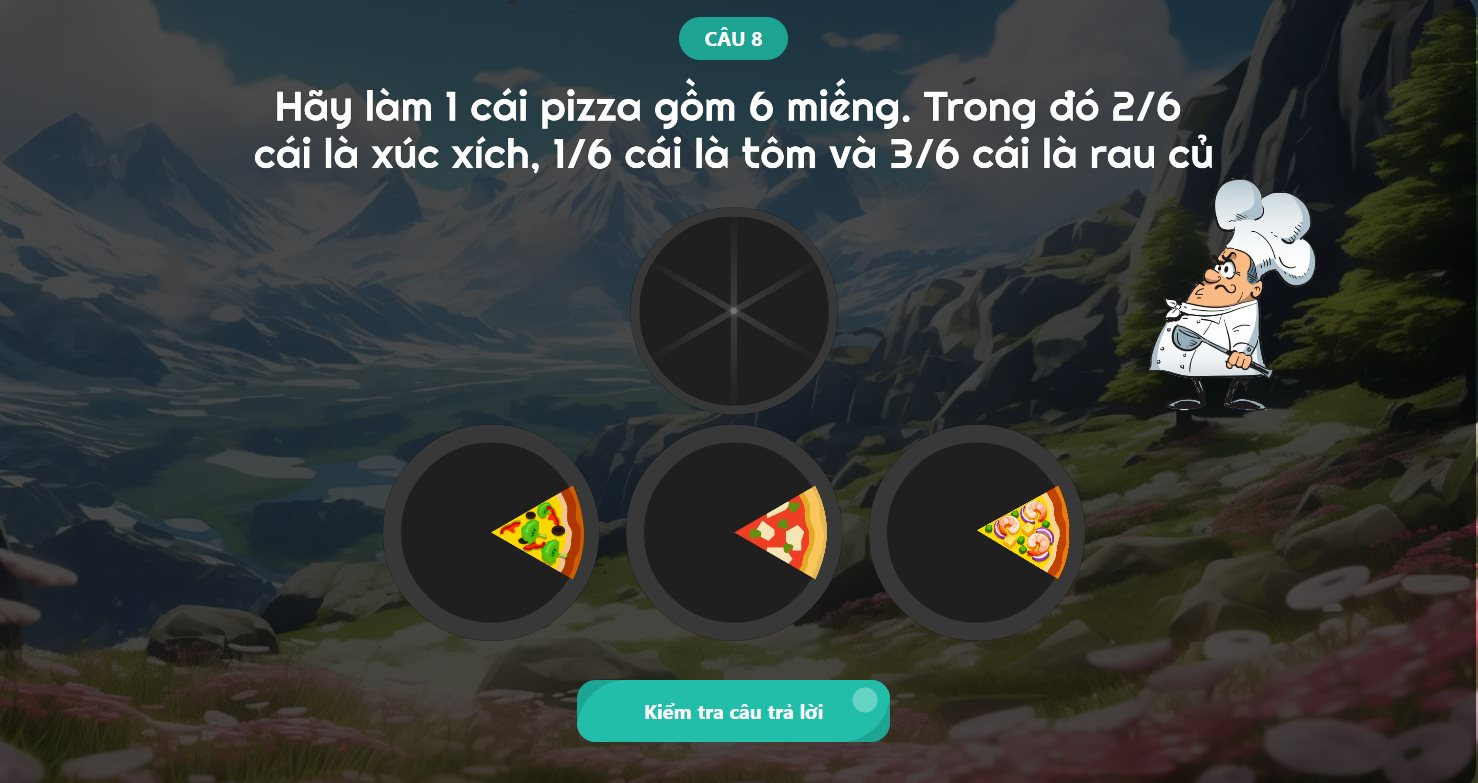
\includegraphics[width=0.9\textwidth]{Image/UI/Exercises/Pizza.jpg}
	\caption{Dạng bài chia pizza}
	\label{fig:pizza}
\end{figure}

\subsubsubsection{Thả chim (Release Bird)}
Dạng bài thả chim có cơ chế tương tự bài trắc nghiệm nhưng được thiết kế với phong cách tương tác sinh động hơn dành cho học sinh lớp nhỏ. Mỗi đáp án được biểu diễn bằng một chiếc lồng chim, phía dưới có bảng hiển thị nội dung đáp án tương ứng. Khi người học chọn đáp án, chiếc lồng sẽ rơi xuống và mở ra để chú chim bay đi, tạo cảm giác vui nhộn và tăng hứng thú học tập.

\begin{figure}[H]
	\centering
	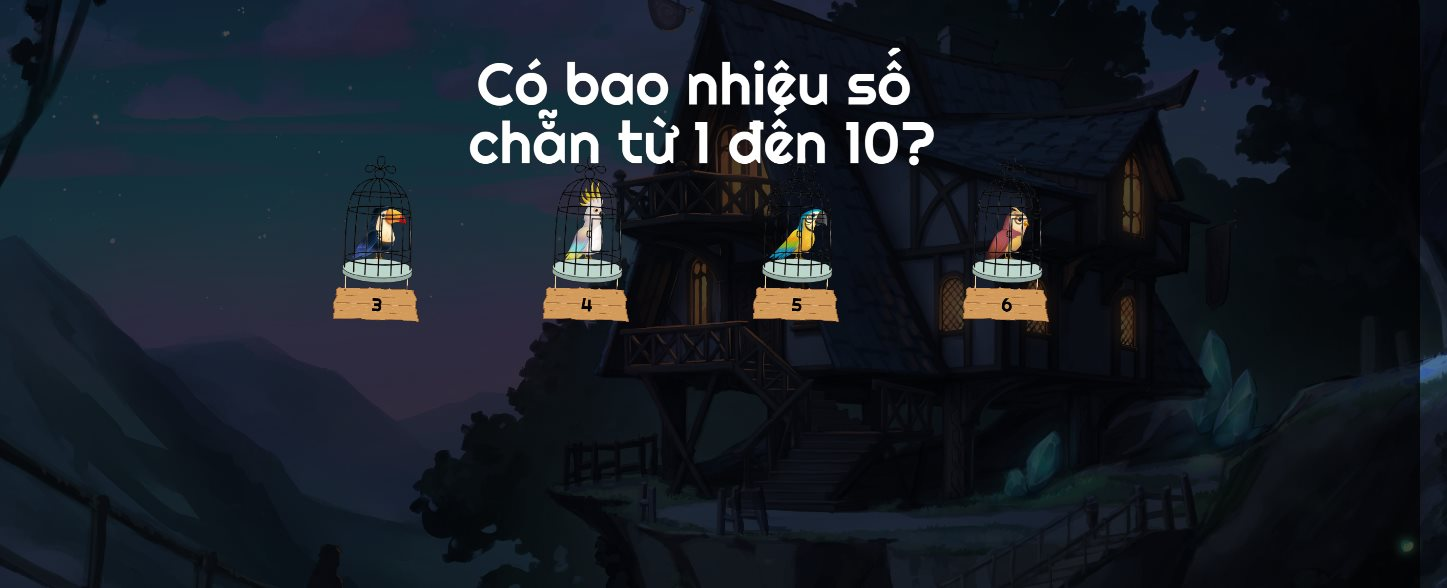
\includegraphics[width=0.9\textwidth]{Image/UI/Exercises/RealeaseBirt.jpg}
	\caption{Dạng bài thả chim}
	\label{fig:release-bird}
\end{figure}

\subsubsubsection{Cân điện tử (Scale)}
Dạng bài cân điện tử yêu cầu học sinh lựa chọn các quả tạ có giá trị khác nhau để đạt đúng khối lượng mục tiêu được đề bài đưa ra. Người học sẽ kéo các quả tạ lên bàn cân và hệ thống sẽ tự động tính tổng khối lượng hiện tại. Một bài toán có thể tồn tại nhiều cách chọn tạ khác nhau miễn tổng khối lượng đạt đúng yêu cầu.

\begin{figure}[H]
	\centering
	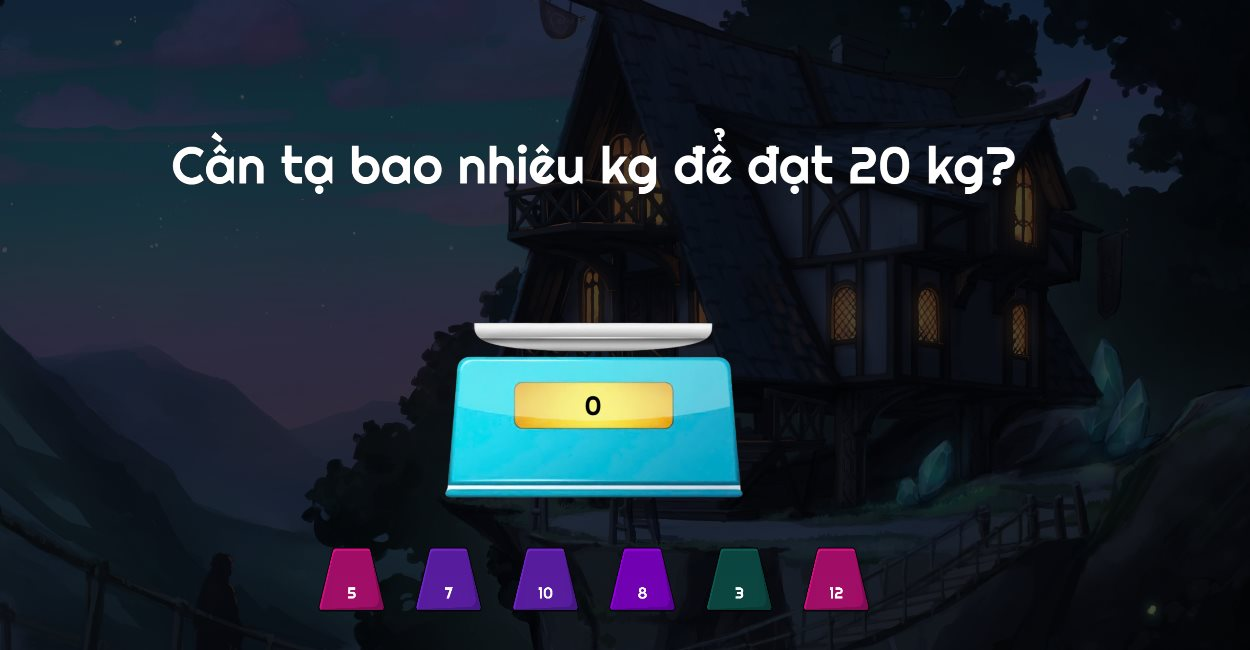
\includegraphics[width=0.9\textwidth]{Image/UI/Exercises/Scale.jpg}
	\caption{Dạng bài cân điện tử}
	\label{fig:scale}
\end{figure}

\subsubsubsection{Tưới cây (Tree)}
Dạng bài tưới cây gồm năm giai đoạn phát triển của cây tương ứng với năm câu hỏi liên tiếp. Mỗi khi trả lời đúng, mây sẽ xuất hiện và tạo mưa giúp cây phát triển sang giai đoạn tiếp theo. Nếu trả lời sai, cây sẽ quay trở lại trạng thái trước đó. Đáp án của mỗi câu hỏi được biểu diễn bằng số lần nhấn nút tương tác. Ví dụ, với bài toán \(2 + X = 5\), học sinh cần nhấn nút ba lần để tạo ra đáp án đúng.

\begin{figure}[H]
	\centering
	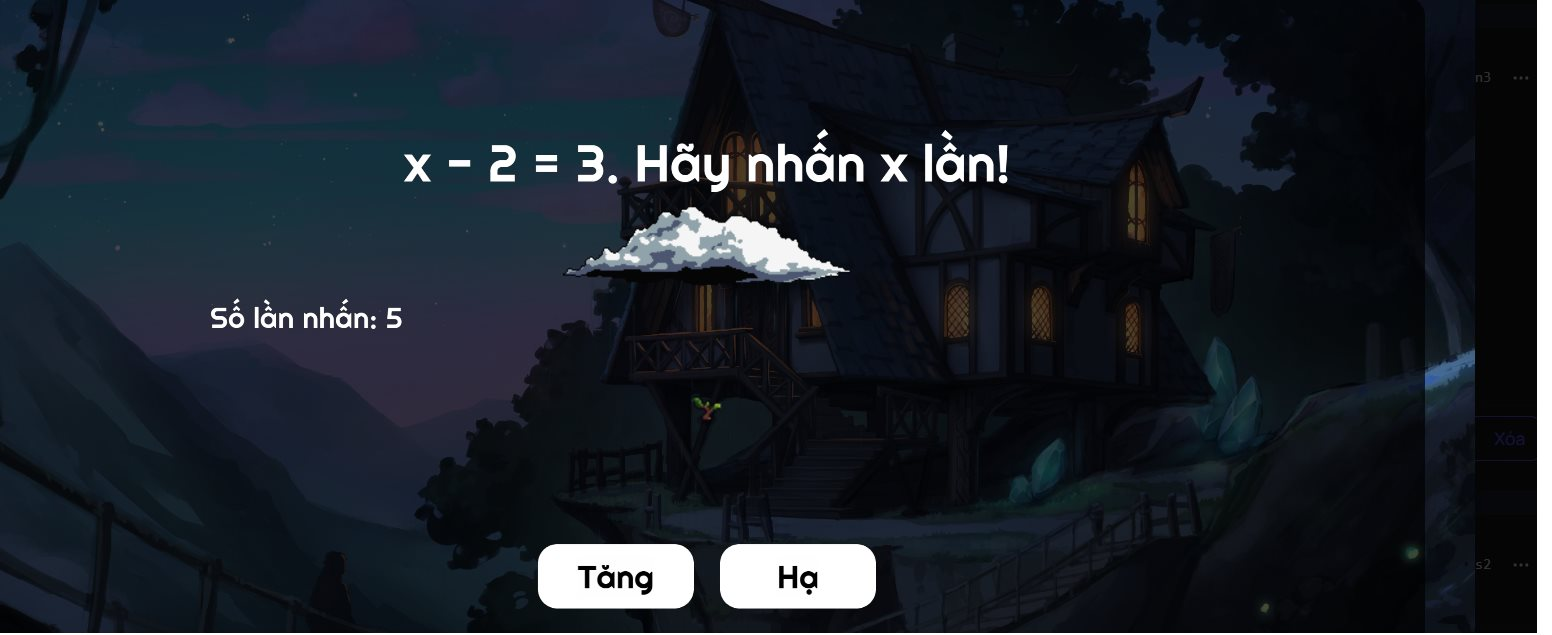
\includegraphics[width=0.9\textwidth]{Image/UI/Exercises/Tree.jpg}
	\caption{Dạng bài tưới cây}
	\label{fig:tree}
\end{figure}

\subsubsubsection{Vẽ hình (Geo)}
Dạng bài vẽ hình được xây dựng theo cơ chế tương tự geoboard. Người học có thể chọn các điểm cố định trên bảng và kéo nối để tạo thành các hình học khác nhau. Hệ thống hỗ trợ nhiều cách vẽ khác nhau cho cùng một đáp án, giúp tăng tính sáng tạo và khả năng tư duy hình học của học sinh.

\begin{figure}[H]
	\centering
	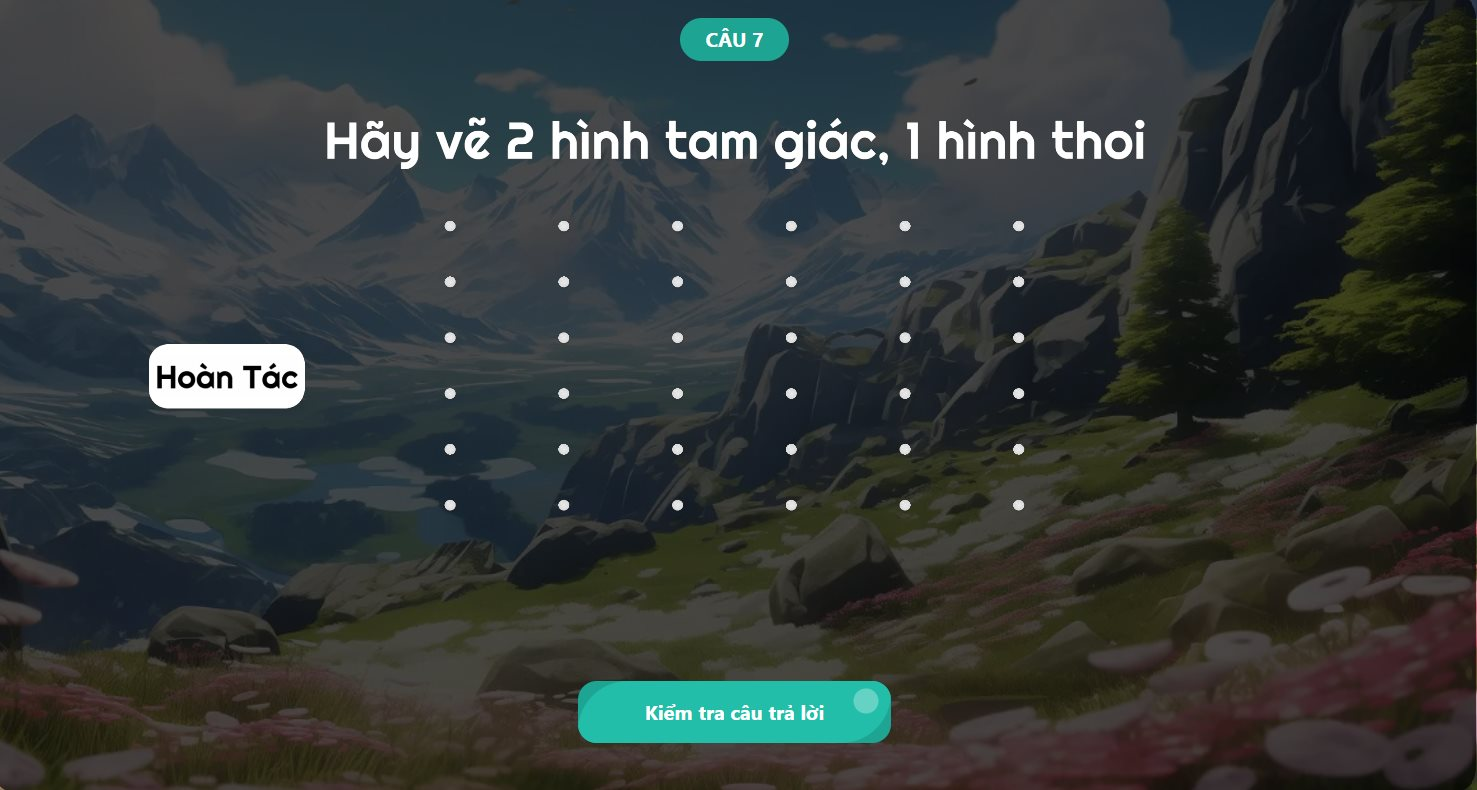
\includegraphics[width=0.9\textwidth]{Image/UI/Exercises/Geo.jpg}
	\caption{Dạng bài vẽ hình}
	\label{fig:geo}
\end{figure}

\subsubsection{Cơ sở học thuật xây dựng bài tập}

Nội dung các bài tập trong hệ thống được xây dựng dựa trên chương trình giáo dục môn Toán cấp Tiểu học của Bộ Giáo dục và Đào tạo. Mỗi chủ đề được phân chia theo ba mức độ nhận thức: \textbf{Nhận biết} (ghi nhớ, tái hiện thông tin), \textbf{Thông hiểu} (giải thích, áp dụng trực tiếp) và \textbf{Vận dụng} (phân tích, giải quyết vấn đề trong tình huống thực tế), nhằm đảm bảo tính phân hóa và phù hợp với từng trình độ học sinh.

% ===================== LỚP 1 =====================
\newpage
\paragraph{Lớp 1}
\renewcommand{\arraystretch}{1.3}
\begin{longtable}{|>{\centering\arraybackslash}m{0.8cm}|m{3.5cm}|>{\centering\arraybackslash}m{2cm}|m{7.5cm}|}
	\hline
	\textbf{STT} & \textbf{Chủ đề} & \textbf{Mức độ} & \textbf{Ví dụ minh họa} \\
	\hline
	\endfirsthead
	\hline
	\textbf{STT} & \textbf{Chủ đề} & \textbf{Mức độ} & \textbf{Ví dụ minh họa} \\
	\hline
	\endhead
	\hline
	\endfoot

	1 & Các số đến 10 và các phép tính cơ bản
	& Nhận biết & Viết các số từ 1 đến 10. (Ví dụ: Viết số 7) \\
	\cline{3-4}
	& & Thông hiểu & Thực hiện phép cộng/trừ đơn giản. ($5+3=?$ hoặc $8-2=?$) \\
	\cline{3-4}
	& & Vận dụng & Giải bài toán có lời văn. (Bạn An có 6 cái kẹo, mẹ cho thêm 4 cái. Hỏi An có tất cả bao nhiêu cái kẹo?) \\
	\hline

	2 & So sánh và các dấu toán học
	& Nhận biết & So sánh số lượng đồ vật. (Nhóm nào nhiều hơn, nhóm nào ít hơn?) \\
	\cline{3-4}
	& & Thông hiểu & Điền dấu thích hợp. ($5 \ldots 9$, điền dấu $<$, $>$, $=$ vào chỗ trống) \\
	\cline{3-4}
	& & Vận dụng & So sánh thực tế. (Bạn Lan có 7 viên bi, bạn Nam có 10 viên bi. Ai có nhiều hơn và nhiều hơn mấy viên?) \\
	\hline

	3 & Hình học cơ bản
	& Nhận biết & Chỉ ra các hình đã học. (Trong các hình sau, đâu là hình tam giác?) \\
	\cline{3-4}
	& & Thông hiểu & Đếm số lượng hình. (Trong hình vẽ này có bao nhiêu hình vuông?) \\
	\cline{3-4}
	& & Vận dụng & Ghép hình để tạo hình mới. (Ghép 2 hình tam giác lại, em được hình gì?) \\
	\hline

	4 & Vị trí và phương hướng
	& Nhận biết & Xác định vị trí. (Con mèo đang ở trên hay dưới cái ghế?) \\
	\cline{3-4}
	& & Thông hiểu & Mô tả vị trí của vật. (Con chim đang bay bên trái cái cây.) \\
	\cline{3-4}
	& & Vận dụng & Vẽ một quả bóng bên phải cái hộp và một bông hoa bên trên quả bóng. \\
	\hline

	5 & Các số có hai chữ số
	& Nhận biết & Viết số có hai chữ số. (Viết số "hai mươi lăm".) \\
	\cline{3-4}
	& & Thông hiểu & Phân tích cấu tạo số. (Trong số 37, số 3 thuộc hàng gì, số 7 thuộc hàng gì?) \\
	\cline{3-4}
	& & Vận dụng & Sắp xếp các số 25, 18, 32, 9 theo thứ tự từ bé đến lớn. \\
	\hline

	6 & Phép cộng, trừ trong phạm vi 100 (không nhớ)
	& Nhận biết & Thực hiện phép tính. ($23+6=?$ hoặc $45-20=?$) \\
	\cline{3-4}
	& & Thông hiểu & Điền số còn thiếu. ($40 + \ldots = 47$) \\
	\cline{3-4}
	& & Vận dụng & Bạn có 28 cái nhãn vở, mua thêm 11 cái. Hỏi bạn có tất cả bao nhiêu cái nhãn vở? \\
	\hline

	7 & Phép cộng, trừ có nhớ trong phạm vi 100
	& Nhận biết & Thực hiện phép tính. ($8+7=?$ hoặc $15-9=?$) \\
	\cline{3-4}
	& & Thông hiểu & Đặt tính rồi tính $19+24$ và $52-18$. \\
	\cline{3-4}
	& & Vận dụng & Lớp 1A có 24 học sinh, lớp 1B có 29 học sinh. Cả hai lớp có bao nhiêu học sinh? \\
	\hline

	8 & Đo lường cơ bản
	& Nhận biết & Dùng thước kẻ đo độ dài của một cây bút chì. \\
	\cline{3-4}
	& & Thông hiểu & An đo bàn được 5 gang, Bình đo được 6 gang. Bàn tay của ai lớn hơn? \\
	\cline{3-4}
	& & Vận dụng & Một sợi dây dài 20 cm, cắt đi 8 cm. Sợi dây còn lại dài bao nhiêu cm? \\
	\hline

	9 & Thời gian và xem đồng hồ
	& Nhận biết & Xem giờ đúng. (Đồng hồ chỉ mấy giờ?) \\
	\cline{3-4}
	& & Thông hiểu & An ăn sáng lúc 7 giờ, đi học lúc 8 giờ. Hoạt động nào diễn ra trước? \\
	\cline{3-4}
	& & Vận dụng & Bây giờ là 10 giờ. Sau 3 tiếng nữa sẽ là mấy giờ? \\
	\hline

	10 & Giải bài toán có lời văn
	& Nhận biết & Tóm tắt bài toán. (Có 5 con chim, 2 con bay đi. Còn lại bao nhiêu con? $5-2=?$) \\
	\cline{3-4}
	& & Thông hiểu & Có 5 quả táo trong giỏ, mẹ bỏ thêm 3 quả. Giỏ có bao nhiêu quả? \\
	\cline{3-4}
	& & Vận dụng & Nhà Mai có 10 con gà, bán 4 con, rồi mua thêm 2 con. Còn lại bao nhiêu con gà? \\
	\hline

	\caption{Các chủ đề toán lớp 1 theo chương trình Bộ GD\&ĐT}
	\label{tab:toan-lop1}
\end{longtable}

% ===================== LỚP 2 =====================
\paragraph{Lớp 2}
\renewcommand{\arraystretch}{1.3}
\begin{longtable}{|>{\centering\arraybackslash}m{0.8cm}|m{3.5cm}|>{\centering\arraybackslash}m{2cm}|m{7.5cm}|}
	\hline
	\textbf{STT} & \textbf{Chủ đề} & \textbf{Mức độ} & \textbf{Ví dụ minh họa} \\
	\hline
	\endfirsthead
	\hline
	\textbf{STT} & \textbf{Chủ đề} & \textbf{Mức độ} & \textbf{Ví dụ minh họa} \\
	\hline
	\endhead
	\hline
	\endfoot

	1 & Ôn tập phép cộng, trừ (có nhớ) trong phạm vi 100
	& Nhận biết & Thực hiện phép tính: $12+8=?$ \\
	\cline{3-4}
	& & Thông hiểu & Đặt tính rồi tính: $34+48$. \\
	\cline{3-4}
	& & Vận dụng & Một cửa hàng bán được 45 chiếc bánh mì buổi sáng, buổi chiều bán thêm 37 chiếc. Hỏi cả ngày bán được bao nhiêu chiếc? \\
	\hline

	2 & Cấu tạo phép tính
	& Nhận biết & Trong phép tính $25+13=38$, hãy chỉ ra số hạng và tổng. \\
	\cline{3-4}
	& & Thông hiểu & Phép tính $50-20=30$: đâu là số bị trừ, số trừ và hiệu? \\
	\cline{3-4}
	& & Vận dụng & Tìm số hạng còn thiếu: $15 + \ldots = 40$. \\
	\hline

	3 & Các số trong phạm vi 1\,000
	& Nhận biết & Đọc số 453. \\
	\cline{3-4}
	& & Thông hiểu & Viết số có hàng trăm là 2, hàng chục là 5, hàng đơn vị là 9. \\
	\cline{3-4}
	& & Vận dụng & Sắp xếp các số 325, 253, 532 theo thứ tự từ bé đến lớn. \\
	\hline

	4 & Phép cộng, trừ trong phạm vi 1\,000
	& Nhận biết & Thực hiện phép tính: $200+50=?$ \\
	\cline{3-4}
	& & Thông hiểu & Đặt tính rồi tính: $435+287$. \\
	\cline{3-4}
	& & Vận dụng & Thư viện có 560 quyển sách, nhà trường mua thêm 250 quyển. Hỏi thư viện có tất cả bao nhiêu quyển? \\
	\hline

	5 & Phép nhân và bảng nhân
	& Nhận biết & Chuyển phép cộng $2+2+2+2$ thành phép nhân. \\
	\cline{3-4}
	& & Thông hiểu & Tính tích của $5 \times 6$. \\
	\cline{3-4}
	& & Vận dụng & Mỗi bạn được phát 5 quyển vở. Hỏi 4 bạn sẽ nhận được bao nhiêu quyển vở? \\
	\hline

	6 & Phép chia và bảng chia
	& Nhận biết & Thực hiện phép chia: $10:2=?$ \\
	\cline{3-4}
	& & Thông hiểu & Phép tính nào đúng? (A) $10:5=2$ hoặc (B) $10:2=5$. \\
	\cline{3-4}
	& & Vận dụng & Có 25 cái kẹo, chia đều cho 5 bạn. Hỏi mỗi bạn được bao nhiêu cái kẹo? \\
	\hline

	7 & Đo lường (Độ dài và Khối lượng)
	& Nhận biết & Đọc và viết các đơn vị đo: 1 kg, 1 m, 1 dm. \\
	\cline{3-4}
	& & Thông hiểu & Đổi đơn vị đo: $1\,\text{m} = \ldots\,\text{dm}$. \\
	\cline{3-4}
	& & Vận dụng & Một khúc gỗ dài 20 m, người ta cưa đi 8 m. Hỏi khúc gỗ còn lại dài bao nhiêu mét? \\
	\hline

	8 & Hình học và đo lường
	& Nhận biết & Chỉ ra đâu là đường thẳng, đường cong, đường gấp khúc. \\
	\cline{3-4}
	& & Thông hiểu & Đo độ dài một đoạn thẳng bằng thước kẻ. \\
	\cline{3-4}
	& & Vận dụng & Tính độ dài đường gấp khúc gồm 3 đoạn thẳng dài lần lượt 20 cm, 15 cm, 10 cm. \\
	\hline

	9 & Thời gian và tiền tệ
	& Nhận biết & Xem đồng hồ chỉ 9 giờ 15 phút. \\
	\cline{3-4}
	& & Thông hiểu & Hôm nay là thứ ba. Hỏi ngày mai là thứ mấy? \\
	\cline{3-4}
	& & Vận dụng & Bây giờ là 8 giờ. Sau 15 phút nữa sẽ là mấy giờ? \\
	\hline

	10 & Thống kê và xác suất
	& Nhận biết & Biểu đồ tranh dưới đây cho biết có bao nhiêu quả táo? \\
	\cline{3-4}
	& & Thông hiểu & Lập bảng kiểm đếm số lượng bạn trai, bạn gái trong lớp. \\
	\cline{3-4}
	& & Vận dụng & Gieo một con xúc xắc: chắc chắn, có thể hay không thể ra mặt có 7 chấm? \\
	\hline

	\caption{Các chủ đề toán lớp 2 theo chương trình Bộ GD\&ĐT}
	\label{tab:toan-lop2}
\end{longtable}

% ===================== LỚP 3 =====================
\paragraph{Lớp 3}
\renewcommand{\arraystretch}{1.3}
\begin{longtable}{|>{\centering\arraybackslash}m{0.8cm}|m{3.5cm}|>{\centering\arraybackslash}m{2cm}|m{7.5cm}|}
	\hline
	\textbf{STT} & \textbf{Chủ đề} & \textbf{Mức độ} & \textbf{Ví dụ minh họa} \\
	\hline
	\endfirsthead
	\hline
	\textbf{STT} & \textbf{Chủ đề} & \textbf{Mức độ} & \textbf{Ví dụ minh họa} \\
	\hline
	\endhead
	\hline
	\endfoot

	1 & Hoàn thiện bảng nhân, bảng chia
	& Nhận biết & $7 \times 8 = ?$ \\
	\cline{3-4}
	& & Thông hiểu & Tìm số bị chia trong phép chia: $\ldots : 4 = 9$. \\
	\cline{3-4}
	& & Vận dụng & Có 35 bông hoa, cắm vào các lọ, mỗi lọ 5 bông. Hỏi cắm được bao nhiêu lọ hoa? \\
	\hline

	2 & Phân số cơ bản
	& Nhận biết & Tô màu vào $\dfrac{1}{3}$ hình tròn sau. \\
	\cline{3-4}
	& & Thông hiểu & Sắp xếp các phân số theo thứ tự từ bé đến lớn: $\dfrac{1}{2}$, $\dfrac{1}{4}$, $\dfrac{1}{3}$. \\
	\cline{3-4}
	& & Vận dụng & Mẹ có 12 quả cam, cho An $\dfrac{1}{4}$ số cam đó. Hỏi mẹ đã cho An bao nhiêu quả cam? \\
	\hline

	3 & Các số trong phạm vi 100\,000
	& Nhận biết & Viết số "mười hai nghìn không trăm năm mươi tư". \\
	\cline{3-4}
	& & Thông hiểu & Phân tích cấu tạo số: 45\,782 gồm bao nhiêu nghìn, trăm, chục, đơn vị? \\
	\cline{3-4}
	& & Vận dụng & Sắp xếp các số 23\,456; 23\,546; 23\,465 theo thứ tự từ lớn đến bé. \\
	\hline

	4 & Cộng, trừ, nhân, chia trong phạm vi 100\,000
	& Nhận biết & $25\,431 + 10\,520 = ?$ \\
	\cline{3-4}
	& & Thông hiểu & Đặt tính rồi tính $15\,328 \times 4$ và $48\,576 : 6$. \\
	\cline{3-4}
	& & Vận dụng & Một xưởng may sản xuất 12\,560 chiếc áo tháng đầu, tháng thứ hai sản xuất nhiều hơn 2\,500 chiếc. Hỏi cả hai tháng sản xuất được bao nhiêu chiếc? \\
	\hline

	5 & Tìm thành phần chưa biết của phép tính
	& Nhận biết & Tìm $x$ trong phép tính $x + 15 = 20$. \\
	\cline{3-4}
	& & Thông hiểu & Tìm $x$ trong phép tính $x : 7 = 8$. \\
	\cline{3-4}
	& & Vận dụng & Tìm $x$ trong phép tính $100 - x = 25 \times 3$. \\
	\hline

	6 & Giải toán với biểu thức và hai bước tính
	& Nhận biết & Tính giá trị của biểu thức: $500 + 50 \times 2$. \\
	\cline{3-4}
	& & Thông hiểu & An có 20 viên bi, Bình có gấp 3 lần số bi của An. Hỏi Bình có bao nhiêu viên bi? \\
	\cline{3-4}
	& & Vận dụng & Một cửa hàng có 500 kg gạo tẻ, đã bán 250 kg và còn lại $\dfrac{1}{2}$ số gạo đã bán. Hỏi ban đầu cửa hàng có bao nhiêu kg gạo? \\
	\hline

	7 & Hình học cơ bản
	& Nhận biết & Đâu là góc vuông, đâu là góc không vuông? \\
	\cline{3-4}
	& & Thông hiểu & Vẽ một đoạn thẳng AB dài 5 cm. \\
	\cline{3-4}
	& & Vận dụng & Vẽ một hình chữ nhật có chiều dài 8 cm và chiều rộng 5 cm. \\
	\hline

	8 & Chu vi và diện tích
	& Nhận biết & Tính chu vi của hình vuông có cạnh dài 5 cm. \\
	\cline{3-4}
	& & Thông hiểu & Tính diện tích của hình chữ nhật có chiều dài 10 cm và chiều rộng 6 cm. \\
	\cline{3-4}
	& & Vận dụng & Một mảnh vườn hình chữ nhật dài 20 m, rộng 15 m. Người ta rào lưới xung quanh. Hỏi cần bao nhiêu mét lưới? \\
	\hline

	9 & Đo lường (Độ dài, khối lượng, dung tích, nhiệt độ)
	& Nhận biết & Viết ký hiệu của đơn vị đo: mililitre. \\
	\cline{3-4}
	& & Thông hiểu & Đổi đơn vị: $3\,\text{kg} = \ldots\,\text{g}$. \\
	\cline{3-4}
	& & Vận dụng & Một xe tải chở 1\,500 kg gạo và thêm 500 kg ngô. Hỏi xe tải chở tất cả bao nhiêu tạ? (biết $1\,\text{tạ} = 100\,\text{kg}$) \\
	\hline

	10 & Thống kê và xác suất
	& Nhận biết & Theo biểu đồ, lớp 2 có bao nhiêu học sinh? \\
	\cline{3-4}
	& & Thông hiểu & Lập bảng thống kê số lượng các loại quả: 3 quả táo, 2 quả cam, 4 quả dứa. \\
	\cline{3-4}
	& & Vận dụng & Khi gieo một đồng xu, khả năng nào sẽ xảy ra: chắc chắn ra mặt sấp, có thể ra mặt sấp, hay không thể ra mặt sấp? \\
	\hline

	\caption{Các chủ đề toán lớp 3 theo chương trình Bộ GD\&ĐT}
	\label{tab:toan-lop3}
\end{longtable}

% ===================== LỚP 4 =====================
\paragraph{Lớp 4}
\renewcommand{\arraystretch}{1.3}
\begin{longtable}{|>{\centering\arraybackslash}m{0.8cm}|m{3.5cm}|>{\centering\arraybackslash}m{2cm}|m{7.5cm}|}
	\hline
	\textbf{STT} & \textbf{Chủ đề} & \textbf{Mức độ} & \textbf{Ví dụ minh họa} \\
	\hline
	\endfirsthead
	\hline
	\textbf{STT} & \textbf{Chủ đề} & \textbf{Mức độ} & \textbf{Ví dụ minh họa} \\
	\hline
	\endhead
	\hline
	\endfoot

	1 & Các số tự nhiên có nhiều chữ số
	& Nhận biết & Đọc và viết số có nhiều chữ số. (Ví dụ: "một trăm hai mươi ba triệu...") \\
	\cline{3-4}
	& & Thông hiểu & Xác định giá trị vị trí. (Ví dụ: Chữ số 5 trong 123\,456\,789 có giá trị là 500\,000.) \\
	\cline{3-4}
	& & Vận dụng & So sánh và sắp xếp các số có nhiều chữ số theo thứ tự. \\
	\hline

	2 & Các phép tính với số tự nhiên
	& Nhận biết & Thực hiện bốn phép tính cơ bản với các số lớn, kể cả phép chia có dư. \\
	\cline{3-4}
	& & Thông hiểu & Vận dụng tính chất giao hoán, kết hợp để tính nhẩm nhanh. (Ví dụ: $25 \times 36 \times 4$) \\
	\cline{3-4}
	& & Vận dụng & Tìm số bị chia, số chia trong phép chia có dư. \\
	\hline

	3 & Số trung bình cộng
	& Nhận biết & Nắm vững công thức tính trung bình cộng. \\
	\cline{3-4}
	& & Thông hiểu & Tính trung bình cộng của dãy số: 10, 20, 30, 40. \\
	\cline{3-4}
	& & Vận dụng & Một đội ngày đầu trồng 200 cây, ngày thứ hai trồng 300 cây. Trung bình mỗi ngày trồng được bao nhiêu cây? \\
	\hline

	4 & Phân số và các phép tính cơ bản
	& Nhận biết & Nhận biết khái niệm phân số: tử số, mẫu số. \\
	\cline{3-4}
	& & Thông hiểu & Rút gọn phân số và quy đồng mẫu số. \\
	\cline{3-4}
	& & Vận dụng & So sánh các phân số khác mẫu số. \\
	\hline

	5 & Các phép tính với phân số
	& Nhận biết & Cộng, trừ, nhân, chia phân số cùng mẫu số. \\
	\cline{3-4}
	& & Thông hiểu & Cộng, trừ phân số khác mẫu số sau khi quy đồng. \\
	\cline{3-4}
	& & Vận dụng & Một tấm vải dài $\frac{3}{4}$ m, cắt đi $\frac{1}{2}$ m. Hỏi tấm vải còn lại dài bao nhiêu mét? \\
	\hline

	6 & Hình học cơ bản
	& Nhận biết & Nhận biết và gọi tên hình bình hành, hình thoi. \\
	\cline{3-4}
	& & Thông hiểu & Phân biệt góc nhọn, góc tù, góc bẹt; đường thẳng vuông góc, song song. \\
	\cline{3-4}
	& & Vận dụng & Vẽ hình theo yêu cầu. \\
	\hline

	7 & Chu vi và diện tích
	& Nhận biết & Công thức tính chu vi và diện tích hình vuông, hình chữ nhật. \\
	\cline{3-4}
	& & Thông hiểu & Chuyển đổi đơn vị đo diện tích (m$^2$, dm$^2$). \\
	\cline{3-4}
	& & Vận dụng & Tính chu vi và diện tích trong tình huống thực tế, kể cả bài toán ghép hình. \\
	\hline

	8 & Đo lường (Khối lượng và thời gian)
	& Nhận biết & Các đơn vị đo khối lượng lớn: yến, tạ, tấn; thời gian: thế kỷ, giây. \\
	\cline{3-4}
	& & Thông hiểu & Chuyển đổi đơn vị. (Ví dụ: $1\,\text{tấn} = \ldots\,\text{kg}$) \\
	\cline{3-4}
	& & Vận dụng & Một xe tải chở 5 tấn hàng, đã dỡ 2 tạ. Trên xe còn lại bao nhiêu kg hàng? \\
	\hline

	9 & Thống kê và biểu đồ
	& Nhận biết & Đọc và hiểu thông tin từ biểu đồ cột. \\
	\cline{3-4}
	& & Thông hiểu & Lập bảng thống kê từ một dãy số liệu. \\
	\cline{3-4}
	& & Vận dụng & Phân tích biểu đồ: lớp nào có nhiều học sinh giỏi nhất? \\
	\hline

	10 & Toán nâng cao và biểu thức
	& Nhận biết & Bài toán tìm hai số khi biết tổng và hiệu. \\
	\cline{3-4}
	& & Thông hiểu & Tính giá trị biểu thức: $a + b \times 5$ khi $a=10$, $b=2$. \\
	\cline{3-4}
	& & Vận dụng & Bài toán rút về đơn vị. (Ví dụ: 3 kg táo hết 60\,000 đồng. Hỏi 5 kg hết bao nhiêu tiền?) \\
	\hline

	\caption{Các chủ đề toán lớp 4 theo chương trình Bộ GD\&ĐT}
	\label{tab:toan-lop4}
\end{longtable}

% ===================== LỚP 5 =====================
\paragraph{Lớp 5}
\renewcommand{\arraystretch}{1.3}
\begin{longtable}{|>{\centering\arraybackslash}m{0.8cm}|m{3.5cm}|>{\centering\arraybackslash}m{2cm}|m{7.5cm}|}
	\hline
	\textbf{STT} & \textbf{Chủ đề} & \textbf{Mức độ} & \textbf{Ví dụ minh họa} \\
	\hline
	\endfirsthead
	\hline
	\textbf{STT} & \textbf{Chủ đề} & \textbf{Mức độ} & \textbf{Ví dụ minh họa} \\
	\hline
	\endhead
	\hline
	\endfoot

	1 & Ôn tập và bổ sung kiến thức
	& Nhận biết & Một đội công nhân sửa đường, ngày đầu sửa được 120 m, ngày thứ hai sửa nhiều hơn ngày đầu 15 m. Hỏi ngày thứ hai sửa được bao nhiêu mét đường? \\
	\cline{3-4}
	& & Thông hiểu & Một tấm vải dài 30 m, đã bán được $\dfrac{2}{3}$ tấm vải. Hỏi còn lại bao nhiêu mét vải? \\
	\cline{3-4}
	& & Vận dụng & Một cửa hàng bán gạo buổi sáng 500 kg, buổi chiều bán $\dfrac{1}{2}$ số gạo buổi sáng. Hỏi cả hai buổi cửa hàng bán được bao nhiêu tạ gạo? \\
	\hline

	2 & Số thập phân
	& Nhận biết & Viết các số: "Năm phẩy bảy mươi lăm" và "Bốn trăm năm mươi sáu phẩy không không tám". \\
	\cline{3-4}
	& & Thông hiểu & Sắp xếp theo thứ tự từ lớn đến bé: 12,3; 12,03; 12,31; 12,13. \\
	\cline{3-4}
	& & Vận dụng & Dùng 3 chữ số 0, 5, 8 và dấu phẩy, hãy viết tất cả các số thập phân có hai chữ số ở phần thập phân và lớn hơn 50. \\
	\hline

	3 & Các phép tính với số thập phân
	& Nhận biết & Thực hiện phép tính: $15{,}4 + 8{,}9 = ?$ \\
	\cline{3-4}
	& & Thông hiểu & Mẹ mua cá hết 56\,500 đồng và mua rau hết 15\,500 đồng, đưa 100\,000 đồng. Hỏi mẹ được trả lại bao nhiêu tiền? \\
	\cline{3-4}
	& & Vận dụng & Một mảnh đất hình chữ nhật dài 25,5 m, chiều rộng bằng $\dfrac{2}{3}$ chiều dài. Tính chu vi và diện tích mảnh đất đó. \\
	\hline

	4 & Tỉ số và tỉ lệ
	& Nhận biết & Một lớp học có 20 bạn nam và 25 bạn nữ. Tìm tỉ số của số bạn nam và số bạn nữ. \\
	\cline{3-4}
	& & Thông hiểu & Lãi suất tiết kiệm là 0,5\% một tháng. Cô Lan gửi 10 triệu đồng. Hỏi sau một tháng cô nhận được bao nhiêu tiền lãi? \\
	\cline{3-4}
	& & Vận dụng & Tổng số tuổi của hai anh em là 36 tuổi. Tuổi em bằng $\dfrac{4}{5}$ tuổi anh. Tính tuổi của mỗi người. \\
	\hline

	5 & Hình học phẳng nâng cao
	& Nhận biết & Một hình tam giác có đáy 10 cm, chiều cao 8 cm. Tính diện tích hình tam giác đó. \\
	\cline{3-4}
	& & Thông hiểu & Một hình tròn có bán kính 5 dm. Tính chu vi và diện tích hình tròn đó. \\
	\cline{3-4}
	& & Vận dụng & Một mảnh đất hình thang có tổng độ dài hai đáy là 40 m, chiều cao 25 m. Tính diện tích mảnh đất. \\
	\hline

	6 & Hình học không gian cơ bản
	& Nhận biết & Một hình lập phương có cạnh 4 cm. Tính thể tích hình lập phương đó. \\
	\cline{3-4}
	& & Thông hiểu & Một hình hộp chữ nhật dài 12 m, rộng 8 m, cao 5 m. Tính diện tích xung quanh và diện tích toàn phần. \\
	\cline{3-4}
	& & Vận dụng & Một bể cá hình hộp chữ nhật dài 1,2 m, rộng 0,8 m, cao 1 m. Người ta đổ nước sao cho mực nước bằng $\dfrac{3}{4}$ chiều cao bể. Tính thể tích nước trong bể. \\
	\hline

	7 & Đo lường
	& Nhận biết & Đổi đơn vị: $12\,\text{tấn} = \ldots\,\text{kg}$. \\
	\cline{3-4}
	& & Thông hiểu & Một xe chở 5 tấn 50 kg gạo, lần đầu dỡ 2\,500 kg. Hỏi trên xe còn lại bao nhiêu tạ gạo? \\
	\cline{3-4}
	& & Vận dụng & Một ô tô đi từ A lúc 7 giờ 30 phút, đến B lúc 10 giờ 15 phút, dọc đường nghỉ 30 phút. Hỏi thời gian ô tô đi thực tế là bao lâu? \\
	\hline

	8 & Toán chuyển động đều
	& Nhận biết & Một người đi bộ vận tốc 5 km/giờ. Hỏi sau 2 giờ đi được bao nhiêu km? \\
	\cline{3-4}
	& & Thông hiểu & Một xe máy đi từ A đến B với vận tốc 40 km/giờ hết 2 giờ, sau đó quay về A với vận tốc 50 km/giờ. Tính thời gian xe đi từ B về A. \\
	\cline{3-4}
	& & Vận dụng & Hai ô tô khởi hành cùng lúc từ A và B (cách nhau 210 km) đi ngược chiều nhau. Vận tốc xe từ A là 50 km/giờ, xe từ B là 60 km/giờ. Hỏi sau bao lâu hai xe gặp nhau? \\
	\hline

	9 & Thống kê và xác suất
	& Nhận biết & Biểu đồ cho biết số học sinh thích môn bóng đá là bao nhiêu? \\
	\cline{3-4}
	& & Thông hiểu & Khối lớp 5 có 150 học sinh, trong đó 60 bạn nữ. Biểu diễn tỉ số phần trăm số bạn nữ và bạn nam bằng biểu đồ quạt. \\
	\cline{3-4}
	& & Vận dụng & Trong một hộp có 5 viên bi đỏ và 3 viên bi xanh. Không nhìn vào hộp, lấy ngẫu nhiên 1 viên. Việc lấy được bi đỏ có chắc chắn, có thể hay không thể xảy ra? \\
	\hline

	10 & Ứng dụng toán học vào thực tiễn
	& Nhận biết & Trên bản đồ tỉ lệ 1:1\,000, khoảng cách A và B là 5 cm. Hỏi khoảng cách thực tế là bao nhiêu mét? \\
	\cline{3-4}
	& & Thông hiểu & Một người gửi tiết kiệm 50 triệu đồng với lãi suất 0,6\% một tháng. Hỏi sau 2 tháng rút cả vốn lẫn lãi được bao nhiêu tiền? \\
	\cline{3-4}
	& & Vận dụng & Bác An mua tivi giá 10 triệu đồng, trả trước 40\%. Số còn lại trả góp trong 5 tháng đều nhau. Hỏi mỗi tháng bác phải trả bao nhiêu tiền? \\
	\hline

	\caption{Các chủ đề toán lớp 5 theo chương trình Bộ GD\&ĐT}
	\label{tab:toan-lop5}
\end{longtable}

\subsubsection{Ánh xạ dạng bài tập với chủ đề học thuật}

Bảng dưới đây thể hiện sự tương ứng giữa 18 dạng bài tập tương tác đã hiện thực và các chủ đề trong chương trình toán tiểu học. Ký hiệu \textbf{C\textit{n}} chỉ chủ đề thứ $n$ theo thứ tự trong bảng của từng lớp.

\renewcommand{\arraystretch}{1.35}
\begin{longtable}{|m{3.5cm}|>{\centering\arraybackslash}m{1.5cm}|>{\centering\arraybackslash}m{1.5cm}|>{\centering\arraybackslash}m{1.5cm}|>{\centering\arraybackslash}m{1.5cm}|>{\centering\arraybackslash}m{1.5cm}|m{3.5cm}|}
	\hline
	\textbf{Dạng bài tập} & \textbf{Lớp 1} & \textbf{Lớp 2} & \textbf{Lớp 3} & \textbf{Lớp 4} & \textbf{Lớp 5} & \textbf{Ghi chú} \\
	\hline
	\endfirsthead
	\hline
	\textbf{Dạng bài tập} & \textbf{Lớp 1} & \textbf{Lớp 2} & \textbf{Lớp 3} & \textbf{Lớp 4} & \textbf{Lớp 5} & \textbf{Ghi chú} \\
	\hline
	\endhead
	\hline
	\endfoot

	Trắc nghiệm \newline (Multiple Choice)
	& C1--C10 & C1--C10 & C1--C10 & C1--C10 & C1--C10
	& Áp dụng cho toàn bộ chủ đề \\
	\hline

	Ghép cặp \newline (Matching)
	& C2, C3 & C5, C6 & C1, C2 & C4, C6 & C4, C5
	& Ghép số, ghép hình, ghép phép tính tương đương \\
	\hline

	Điền số \newline (Fill in the Blanks)
	& C1, C6, C7 & C1, C2, C4 & C4, C5 & C2, C3 & C1, C3
	& Điền kết quả phép tính, tìm thành phần còn thiếu \\
	\hline

	Kéo thả \newline (Drag and Drop)
	& C1, C5 & C3, C4 & C3, C4 & C1, C2 & C2, C3
	& Điền số vào biểu thức, sắp xếp dãy số \\
	\hline

	Phân loại \newline (Grouping)
	& C1, C5 & C3 & C3 & C1 & C2
	& Phân loại chẵn/lẻ, phân loại hình, phân loại theo nhóm \\
	\hline

	Đúng/Sai \newline (True/False)
	& C2, C6, C7 & C1, C4, C5, C6 & C1, C4, C5 & C2, C4, C5 & C1, C3, C4
	& Kiểm tra tính đúng đắn của một phép tính hoặc mệnh đề so sánh \\
	\hline

	Tổ hợp Burger \newline (Burger)
	& -- & C10 & C10 & C10 & C9
	& Thống kê, xác suất tổ hợp \\
	\hline

	Xe buýt \newline (Bus)
	& C6 & C1, C4 & C4 & C2 & --
	& Cộng số tròn chục/tròn trăm; xếp hàng lên xe \\
	\hline

	Bắt chim \newline (Catch Bird)
	& C1, C6, C7 & C1, C4, C5 & C1, C4 & C2, C3 & C1, C3
	& Dạng tổng quát; biểu diễn nhiều dạng toán bằng cơ chế bắt chim \\
	\hline

	Đồng hồ \newline (Clock)
	& C9 & C9 & -- & C8 & C7
	& Đọc giờ kim, giờ số; tính thời gian \\
	\hline

	Đổi tiền xu \newline (Coin)
	& -- & C9 & -- & C8 & C10
	& Nhận biết mệnh giá, đổi tiền, tính toán với tiền tệ \\
	\hline

	Viên bi \newline (Gumball)
	& C1, C2 & C10 & C10 & C9 & C9
	& Đếm, so sánh số lượng; thống kê trực quan \\
	\hline

	Cân thủ công \newline (Manual Scale)
	& C2 & C7 & C9 & C8 & C7
	& So sánh lớn hơn/bé hơn/bằng nhau qua cân \\
	\hline

	Chia pizza \newline (Pizza)
	& -- & -- & C2 & C4, C5 & C4
	& Làm quen phân số, tỉ lệ qua hình ảnh trực quan \\
	\hline

	Thả chim \newline (Release Bird)
	& C1--C10 & C1--C10 & C1--C10 & C1--C10 & C1--C10
	& Áp dụng cho toàn bộ chủ đề \\
	\hline

	Cân điện tử \newline (Scale)
	& C6, C7 & C1, C4 & C4 & C2 & C3
	& Cộng/trừ qua cân bằng; có thể có nhiều đáp án đúng \\
	\hline

	Tưới cây \newline (Tree)
	& C10 & C2 & C6 & C10 & C10
	& Bài toán nhiều bước; tưới từng bước để hoàn thành \\
	\hline

	Vẽ hình \newline (Geo)
	& C3 & C8 & C7, C8 & C6, C7 & C5
	& Vẽ hình học; tính chu vi, diện tích \\
	\hline

	\caption{Ánh xạ giữa 18 dạng bài tập và chủ đề chương trình Bộ GD\&ĐT}
	\label{tab:exercise-mapping}
\end{longtable}

Kết quả phân tích bảng ánh xạ cho thấy hệ thống bài tập đạt được độ bao phủ toàn diện trên toàn bộ chương trình toán tiểu học. Với \textbf{18 dạng tương tác} được phân phối trải rộng qua \textbf{5 khối lớp} và \textbf{10 chủ đề học thuật} mỗi lớp, mọi đơn vị kiến thức trong chương trình của Bộ Giáo dục và Đào tạo đều có ít nhất một dạng bài tập phù hợp để luyện tập.
Điểm nhấn quan trọng trong thiết kế là hệ thống đề cao \textbf{tư duy linh hoạt}: nhiều dạng bài chấp nhận \textbf{nhiều cách giải khác nhau} miễn là kết quả cuối cùng là đúng, phản ánh đúng bản chất của toán học là khuyến khích học sinh tự tìm con đường tư duy của mình thay vì rập khuôn một đáp án duy nhất.
Ba mức độ nhận thức \textbf{Nhận biết -- Thông hiểu -- Vận dụng} được duy trì xuyên suốt theo đúng chuẩn chương trình của Bộ Giáo dục và Đào tạo, giúp hệ thống phục vụ toàn dải trình độ: từ học sinh mới làm quen khái niệm đến học sinh cần thử thách ở mức phân tích và giải quyết vấn đề thực tế. Sự kết hợp giữa độ bao phủ rộng theo chương trình, tính chuyên biệt theo từng miền kiến thức và triết lý tôn trọng tư duy đa hướng là nền tảng để hệ thống không chỉ dạy toán mà còn \textbf{rèn luyện cách suy nghĩ} cho học sinh tiểu học.

